\documentclass[12pt]{report}
\usepackage{suthesis}

%\documentstyle[12pt,suthesis]{report}



% -- Imports --
% (general libraries)
\usepackage{times,latexsym,amsfonts,amssymb,amsmath,graphicx,url,bbm,rotating}
\usepackage{enumitem,multirow,hhline,stmaryrd,bussproofs,mathtools,siunitx,arydshln}
\usepackage{booktabs,xcolor,csquotes,calligra}
\usepackage{dsfont,xspace}
\usepackage{rotating}
% (custom libraries)
\usepackage{fitch}
\usepackage{amsmath}

% (inline references)
\usepackage{natbib}
% (tikz)
\usepackage{tikz}
\usepackage{tikz-dependency,pifont}
\usetikzlibrary{shapes.arrows,chains,positioning,automata,trees,calc}
\usetikzlibrary{patterns,matrix}
\usetikzlibrary{decorations.pathmorphing,decorations.markings}
% (print algorithms)
%\usepackage[ruled,lined,linesnumbered]{algorithm2e}
% (custom)
\input std-macros.tex
\input macros.tex	
% (paper compilation hacks)
\def\newcite#1{\citet{#1}}
\def\cite#1{\citep{#1}}
%\def\newcite#1{\textcite{#1}}
%\def\cite#1{\autocite{#1}}
\definecolor{darkblue}{rgb}{0.0,0.0,0.4}

% Common hyphenations
\hyphenation{Text-Runner}
\hyphenation{Verb-Ocean}

\newenvironment{tightitemize}%
  {\begin{itemize}[topsep=0pt, partopsep=0pt] %
    \setlength{\parskip}{0pt}%
    }%
  {\end{itemize}}

%\bibliographystyle{plainnat}

\usepackage{epigraph}
\renewcommand{\epigraphsize}{\normalsize}
\setlength{\epigraphwidth}{0.8\textwidth}

\newcommand{\bleu}{{{\sc Bleu}}\xspace}
\newcommand{\meteor}{{{\sc Meteor}}\xspace}
\newcommand{\camready}[1]{{{#1}}}

\newcommand{\eos}{{$\langle \mathrm{eos}\rangle$}\xspace}
\newcommand{\bos}{{$\langle \mathrm{bos}\rangle$}\xspace}
\newcommand{\unk}{{$\langle \mathrm{unk}\rangle$}\xspace}

\newcommand{\copynet}{{\textsc{CopyNet}}\xspace}

\newcommand{\uunk}{{\langle \mathrm{unk}\rangle}}
\newcommand{\sts}{{{\textsc{Seq2Seq}}}\xspace}
\newcommand{\dbleu}{{$\Delta${\sc Bleu}}\xspace}
\newcommand{\fix}{\marginpar{FIX}}
\newcommand{\new}{\marginpar{NEW}}
\newcommand{\MINUS}{}
\DeclareMathOperator{\softmax}{\text{softmax}}
\DeclareMathOperator{\argsort}{\text{argsort}}
\newcommand{\ssoftmax}{\mathop{\softmax}\limits}
\usepackage{tabularx}
\usepackage{tabulary}
\usepackage{comment}

\newcommand{\tabincell}[2]{\begin{tabular}{@{}#1@{}}#2\end{tabular}}



% special packages
\usepackage{algorithm}
\usepackage{mathrsfs}
\usepackage{enumitem}
\usepackage{subfigure}
\usepackage{amssymb}
\usepackage[noend]{algpseudocode}
\usepackage{wrapfig,lipsum,booktabs}
\usepackage{booktabs, caption}
\usepackage{tabularx}
\usepackage{listliketab}
\usepackage{lipsum} 
\usepackage{float}
\usepackage{bm}
\usepackage{relsize}
\usepackage{footnote}
\usepackage{bbding}

\usepackage{kotex}

\usepackage{textcomp}
\usepackage{url}
\usepackage{hyperref}
\urlstyle{same}
\newcommand{\alert}[1]{\textcolor{red}{#1}}
\newcommand{\sidebysidecaption}[4]{%
%\RaggedRight%
  \begin{minipage}[t]{#1}
    \vspace*{0pt}
    #3
  \end{minipage}
  \hfill%
  \begin{minipage}[t]{#2}
    \vspace*{0pt}
    #4
\end{minipage}%
}
%\aclfina


% other definition used in copynet
% Miguel A. Carreira-Perpinan's LaTeX macros.
% Time-stamp: <07/02/08 02:40:12 miguel>

% Definitions that require only standard LaTeX2e things

% Letters used for matrices and vectors (boldface), for functions (roman), etc.
\newcommand{\A}{\ensuremath{\mathbf{A}}}
\newcommand{\B}{\ensuremath{\mathbf{B}}}
\newcommand{\C}{\ensuremath{\mathbf{C}}}
%\newcommand{\D}{\ensuremath{\mathbf{D}}}
%\newcommand{\E}{\ensuremath{\mathbf{E}}}
\newcommand{\F}{\ensuremath{\mathbf{F}}}
\newcommand{\G}{\ensuremath{\mathbf{G}}}
\newcommand{\HH}{\ensuremath{\mathbf{H}}}
\newcommand{\I}{\ensuremath{\mathbf{I}}}
\newcommand{\J}{\ensuremath{\mathbf{J}}}
\newcommand{\K}{\ensuremath{\mathbf{K}}}
\newcommand{\LL}{\ensuremath{\mathbf{L}}}
\newcommand{\M}{\ensuremath{\mathbf{M}}}
\newcommand{\N}{\ensuremath{\mathbf{N}}}
\newcommand{\OO}{\ensuremath{\mathbf{O}}}
\newcommand{\PP}{\ensuremath{\mathbf{P}}}
\newcommand{\Q}{\ensuremath{\mathbf{Q}}}
%\newcommand{\R}{\ensuremath{\mathbf{R}}} % PROSPER defines \R
\newcommand{\RR}{\ensuremath{\mathbf{R}}}
\renewcommand{\SS}{\ensuremath{\mathbf{S}}}
%\newcommand{\T}{\ensuremath{\mathbf{T}}}
\newcommand{\U}{\ensuremath{\mathbf{U}}}
\newcommand{\V}{\ensuremath{\mathbf{V}}}
\newcommand{\W}{\ensuremath{\mathbf{W}}}
\newcommand{\X}{\ensuremath{\mathbf{X}}}
\newcommand{\Y}{\ensuremath{\mathbf{Y}}}
%\newcommand{\Z}{\ensuremath{\mathbf{Z}}}
\renewcommand{\aa}{\ensuremath{\mathbf{a}}}
\renewcommand{\b}{\ensuremath{\mathbf{b}}}
\renewcommand{\c}{\ensuremath{\mathbf{c}}}
\newcommand{\dd}{\ensuremath{\mathbf{d}}}
\newcommand{\e}{\ensuremath{\mathbf{e}}}
\newcommand{\f}{\ensuremath{\mathbf{f}}}
\newcommand{\g}{\ensuremath{\mathbf{g}}}
\newcommand{\h}{\ensuremath{\mathbf{h}}}
%\newcommand{\bk}{\ensuremath{\mathbf{k}}}
%newcommand{\bl}{\ensuremath{\mathbf{l}}}
\newcommand{\m}{\ensuremath{\mathbf{m}}}
\newcommand{\n}{\ensuremath{\mathbf{n}}}
%\newcommand{\p}{\ensuremath{\mathbf{p}}}
\newcommand{\q}{\ensuremath{\mathbf{q}}}
\newcommand{\rr}{\ensuremath{\mathbf{r}}}
\newcommand{\sss}{\ensuremath{\mathbf{s}}}  % TIPA defines \s and LaTeX \ss!
\renewcommand{\t}{\ensuremath{\mathbf{t}}}
\newcommand{\uu}{\ensuremath{\mathbf{u}}}
\newcommand{\vv}{\ensuremath{\mathbf{v}}}
%\renewcommand{\v}{\ensuremath{\mathbf{v}}}
%\newcommand{\w}{\ensuremath{\mathbf{w}}}
\newcommand{\x}{\ensuremath{\mathbf{x}}}
\newcommand{\y}{\ensuremath{\mathbf{y}}}
\newcommand{\z}{\ensuremath{\mathbf{z}}}
\newcommand{\0}{\ensuremath{\mathbf{0}}}

\newcommand{\bdelta}{\ensuremath{\boldsymbol{\delta}}}
\newcommand{\binfty}{\ensuremath{\boldsymbol{\infty}}}
\newcommand{\bkappa}{\ensuremath{\boldsymbol{\kappa}}}
\newcommand{\blambda}{\ensuremath{\boldsymbol{\lambda}}}

\newcommand{\bDelta}{\ensuremath{\boldsymbol{\Delta}}}
\newcommand{\bLambda}{\ensuremath{\boldsymbol{\Lambda}}}
\newcommand{\bPhi}{\ensuremath{\boldsymbol{\Phi}}}
\newcommand{\bPi}{\ensuremath{\boldsymbol{\Pi}}}
\newcommand{\bPsi}{\ensuremath{\boldsymbol{\Psi}}}
\newcommand{\bSigma}{\ensuremath{\boldsymbol{\Sigma}}}
\newcommand{\bTheta}{\ensuremath{\boldsymbol{\Theta}}}
\newcommand{\bXi}{\ensuremath{\boldsymbol{\Xi}}}
\newcommand{\bUpsilon}{\ensuremath{\boldsymbol{\Upsilon}}}

% Blackboard bold
\newcommand{\bbC}{\ensuremath{\mathbb{C}}}
\newcommand{\bbH}{\ensuremath{\mathbb{H}}}
\newcommand{\bbN}{\ensuremath{\mathbb{N}}}
\newcommand{\bbR}{\ensuremath{\mathbb{R}}}
\newcommand{\bbS}{\ensuremath{\mathbb{S}}}
\newcommand{\bbZ}{\ensuremath{\mathbb{Z}}}

% Calligraphic
\newcommand{\calA}{\ensuremath{\mathcal{A}}}
\newcommand{\calB}{\ensuremath{\mathcal{B}}}
\newcommand{\calC}{\ensuremath{\mathcal{C}}}
\newcommand{\calD}{\ensuremath{\mathcal{D}}}
\newcommand{\calE}{\ensuremath{\mathcal{E}}}
\newcommand{\calF}{\ensuremath{\mathcal{F}}}
\newcommand{\calG}{\ensuremath{\mathcal{G}}}
\newcommand{\calH}{\ensuremath{\mathcal{H}}}
\newcommand{\calI}{\ensuremath{\mathcal{I}}}
\newcommand{\calJ}{\ensuremath{\mathcal{J}}}
\newcommand{\calL}{\ensuremath{\mathcal{L}}}
\newcommand{\calM}{\ensuremath{\mathcal{M}}}
\newcommand{\calN}{\ensuremath{\mathcal{N}}}
\newcommand{\calO}{\ensuremath{\mathcal{O}}}
\newcommand{\calP}{\ensuremath{\mathcal{P}}}
\newcommand{\calR}{\ensuremath{\mathcal{R}}}
\newcommand{\calS}{\ensuremath{\mathcal{S}}}
\newcommand{\calT}{\ensuremath{\mathcal{T}}}
\newcommand{\calU}{\ensuremath{\mathcal{U}}}
\newcommand{\calV}{\ensuremath{\mathcal{V}}}
\newcommand{\calW}{\ensuremath{\mathcal{W}}}
\newcommand{\calX}{\ensuremath{\mathcal{X}}}
\newcommand{\calY}{\ensuremath{\mathcal{Y}}}

% Relational operators
% \bydef puts ``def'' over the equals sign and means ``is by definition
% equal to''. Another possibility is to use the \triangleq symbol.
\newcommand{\bydef}{\stackrel{\mathrm{\scriptscriptstyle def}}{=}}
% \simbydef puts ``def'' over the ~ sign and means ``is by definition
% distributed as''.
\newcommand{\simbydef}{\stackrel{\mathrm{\scriptscriptstyle def}}{\sim}}
\newcommand{\proptobydef}{\stackrel{\mathrm{\scriptscriptstyle def}}{\propto}}

% Other functions
\newcommand{\abs}[1]{\left\lvert#1\right\rvert}
\newcommand{\norm}[1]{\left\lVert#1\right\rVert}

% Left superscript
% (from http://www.maths.univ-rennes1.fr/~edix/sgahtml/typesetting_rules.html)
\newcommand{\leftexp}[2]{{\vphantom{#2}}^{#1}{#2}}

% Box of text (for pictures, tables, etc.), without frames. Arguments:
%   #1: separation between rows of text as a multiple of LaTeX's default
%       (optional, default 1).
%   #2: position (one of t, b, c).
%   #3: format (one of l, r, c or even p{2cm}).
%   #4: text, which can include line breaks (\\).
\newcommand{\caja}[4][1]{{%
    \renewcommand{\arraystretch}{#1}%
    \begin{tabular}[#2]{@{}#3@{}}%
      #4%
    \end{tabular}%
    }}

% The amsart class has its own \keywords command, in which case we
% don't replace it.
\providecommand{\keywords}[1]{\vspace*{0.5\baselineskip}\par\noindent\textbf{Keywords:} #1}

% The logos (AmSLaTeX, BibTeX, etc.) are defined in texnames.sty.

% List environments
%
% "simplelist": useful for compact lists. Use it instead of "itemize".
% Optional argument: the bullet (default \triangleright). Other nice
% bullets are available in the Zapf Dingbats font (e.g. \ding{166} in
% the pifont package).
%
\newenvironment{simplelist}[1][$\triangleright$]%
{%
\begin{list}{#1}{
\vspace{-\topsep}
\vspace{-\partopsep}
\setlength{\itemindent}{0cm}
\setlength{\rightmargin}{0cm}
\setlength{\listparindent}{0cm}
\settowidth{\labelwidth}{#1}
\setlength{\leftmargin}{\labelwidth}
\addtolength{\leftmargin}{\labelsep}
\setlength{\itemsep}{0cm}
%\setlength{\leftmargin}{0cm}
%\setlength{\labelwidth}{0cm}
}%
}%
{%
\end{list}
\vspace{-\topsep}
\vspace{-\partopsep}
}

%
% enumthm: an enumerated list intended to appear in theorems and not
% to be nested. Each item is numbered in Roman numerals in parentheses.
% A suitable way to refer to an item is:
% Theorem~\ref{thm:pithagoras}(\ref{en:triangle}) states...
\newenvironment{enumthm}%
{\begin{enumerate}%
\renewcommand{\theenumi}{\roman{enumi}}%
\renewcommand{\labelenumi}{(\theenumi)}}%
{\end{enumerate}}

% Commands for the hyperref package (they also require the url package).
% In all cases the typesetting style is tt by default but can be changed
% with the \urlstyle command, e.g. \urlstyle{tt}.
%
% \MACPhref[text]{link} typesets text (default = link) in tt and
% hyperlinks to link, e.g. \MACPhref{http://www.dcs.shef.ac.uk/~miguel}.
\newcommand{\MACPhref}[2][\DefaultOpt]{\def\DefaultOpt{#2}%
  \href{#2}{\url{#1}}}
%
% \MACPmailto[text]{email} typesets text (default = email) in tt and
% hyperlinks to email as mailto:email, e.g. \MACPmailto{miguel@dcs.shef.ac.uk}.
\newcommand{\MACPmailto}[2][\DefaultOpt]{\def\DefaultOpt{#2}%
  \href{mailto:#2}{\url{#1}}}

% Hyphenation
\hyphenation{elec-tro-pa-la-tog-ra-phy}

% From the amsbook.cls file version 2.04
\hyphenation{acad-e-my acad-e-mies af-ter-thought anom-aly anom-alies
an-ti-deriv-a-tive an-tin-o-my an-tin-o-mies apoth-e-o-ses
apoth-e-o-sis ap-pen-dix ar-che-typ-al as-sign-a-ble as-sist-ant-ship
as-ymp-tot-ic asyn-chro-nous at-trib-uted at-trib-ut-able bank-rupt
bank-rupt-cy bi-dif-fer-en-tial blue-print busier busiest
cat-a-stroph-ic cat-a-stroph-i-cally con-gress cross-hatched data-base
de-fin-i-tive de-riv-a-tive dis-trib-ute dri-ver dri-vers eco-nom-ics
econ-o-mist elit-ist equi-vari-ant ex-quis-ite ex-tra-or-di-nary
flow-chart for-mi-da-ble forth-right friv-o-lous ge-o-des-ic
ge-o-det-ic geo-met-ric griev-ance griev-ous griev-ous-ly
hexa-dec-i-mal ho-lo-no-my ho-mo-thetic ideals idio-syn-crasy
in-fin-ite-ly in-fin-i-tes-i-mal ir-rev-o-ca-ble key-stroke
lam-en-ta-ble light-weight mal-a-prop-ism man-u-script mar-gin-al
meta-bol-ic me-tab-o-lism meta-lan-guage me-trop-o-lis
met-ro-pol-i-tan mi-nut-est mol-e-cule mono-chrome mono-pole
mo-nop-oly mono-spline mo-not-o-nous mul-ti-fac-eted mul-ti-plic-able
non-euclid-ean non-iso-mor-phic non-smooth par-a-digm par-a-bol-ic
pa-rab-o-loid pa-ram-e-trize para-mount pen-ta-gon phe-nom-e-non
post-script pre-am-ble pro-ce-dur-al pro-hib-i-tive pro-hib-i-tive-ly
pseu-do-dif-fer-en-tial pseu-do-fi-nite pseu-do-nym qua-drat-ic
quad-ra-ture qua-si-smooth qua-si-sta-tion-ary qua-si-tri-an-gu-lar
quin-tes-sence quin-tes-sen-tial re-arrange-ment rec-tan-gle
ret-ri-bu-tion retro-fit retro-fit-ted right-eous right-eous-ness
ro-bot ro-bot-ics sched-ul-ing se-mes-ter semi-def-i-nite
semi-ho-mo-thet-ic set-up se-vere-ly side-step sov-er-eign spe-cious
spher-oid spher-oid-al star-tling star-tling-ly sta-tis-tics
sto-chas-tic straight-est strange-ness strat-a-gem strong-hold
sum-ma-ble symp-to-matic syn-chro-nous topo-graph-i-cal tra-vers-a-ble
tra-ver-sal tra-ver-sals treach-ery turn-around un-at-tached
un-err-ing-ly white-space wide-spread wing-spread wretch-ed
wretch-ed-ly Eng-lish Euler-ian Feb-ru-ary Gauss-ian
Hamil-ton-ian Her-mit-ian Jan-u-ary Japan-ese Kor-te-weg
Le-gendre Mar-kov-ian Noe-ther-ian No-vem-ber Rie-mann-ian Sep-tem-ber}

%%% Local Variables: 
%%% mode: latex
%%% TeX-master: t
%%% End: 


% -- Document --
\begin{document}

% Title
\title{Efficient Neural Machine Translation}
\author{Jiatao Gu}
\principaladviser{Victor O.K. Li}
\firstreader{Maggie Li}
\secondreader{Kaibin Huang}
\thirdreader{Laurence Young}

% Preface
\beforepreface
\input preface.tex
\input ack.tex
\afterpreface

\chapter{Introduction}
\label{intro}
\epigraph{Translation is that which transforms everything so that nothing changes.}{Grass Günter.}

The dream of automatic translation that builds the communication bridge between people from different civilizations dates back to thousands of years (see Fig.~\ref{cp1.fig.babel}). The ability of an algorithm that are able to translate between any human languages smoothly and accurately has always been a test that an artificial intelligence (AI) is capable of understanding human languages. We will start from a brief review of the research of modern automatic machine translation and then step to our main focus: building an {\it efficient} neural machine translation system.

\section{A Brief Review of Machine Translation (MT)}
For the past decades, researchers devoted to proposing practical plans since 1950s.
\begin{figure}[t]
	\centering
	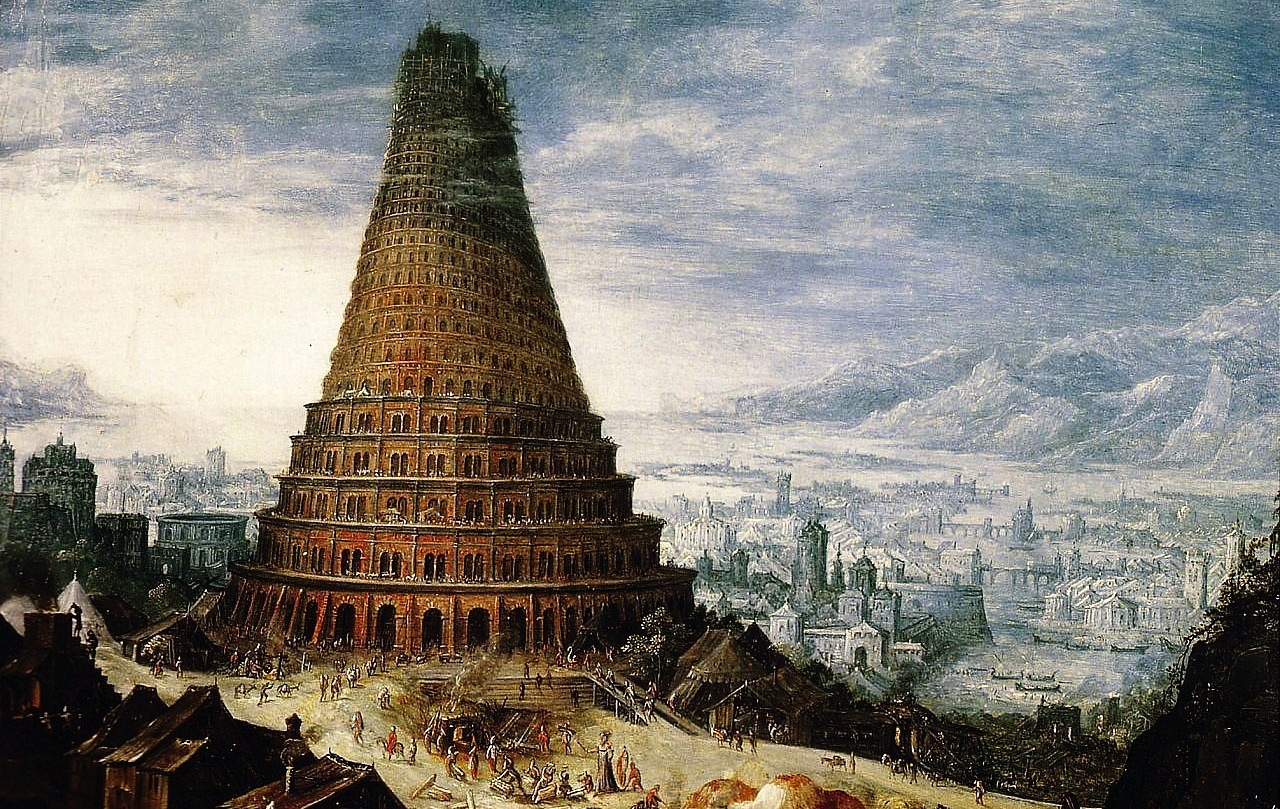
\includegraphics[width=1\linewidth]{figs/intro/tower_of_babel.jpg}
	\caption{\label{cp1.fig.babel}The aim in building Babel and a Tower to “reach into heaven” was to prevent the people from being “scattered abroad over the face of the whole earth” (Genesis 11:4). }
\end{figure}

\paragraph{Rule-based MT} the earliest machine translation systems are rule-based, which requires not only a word-by-word dictionary, but linguistics to design specific translation rules language by language. Although due to its fragility, the rule-based system easily fails to translate correctly to the countless special cases in human languages, rule-based system can usually produce translation in good grammar structure.

\paragraph{Example-based MT}
the example-based machine translation (EBMT)~\citep{Zhang2005AnEP,callison2005scaling,phillips2012modeling} are distinct from the rule-based model which translates new sentences not based on rules, but reference to stored similar translation examples as reference. In a more practical way, it indexes parallel corpora with suffix arrays and retrieves exact matched translation segments on the fly at test time. %However, to the best of our knowledge, SEG-NMT is the first work incorporating any attention-based neural machine translation architectures and can be trained end-to-end efficiently, showing superior performance and scalability compared to the conventional statistical EBMT. 


\paragraph{Statistical MT} another trend of machine translation is the statistical machine translation. Similar to EBMT, SMT does not rely on manually mined translation rules. For example, one of the most successful statistical methods,  phrase-based statistical machine translation (PBMT), first builds a phrase table from a large corpora, which later is used to output translation as searching the most proper sequence of paired phrases that fits to an external language model.

\paragraph{Neural MT}
Till recent years, with the general success of artificial intelligence (AI) and the emergence of neural network models, a.k.a. Deep Learning, neural machine translation (NMT)~\cite{sutskever2014sequence,bahdanau2014neural,vaswani2017attention} , as the new generation of machine translation framework has achieved the state-of-the-art~\cite{wu2016google} and even human-level translation performance in some languages~\cite{hassan-hp}.
Different from prior work in SMT, NMT does not use an explicit language model, but directly model machine translation as a conditional language model via function approximation.  
The impressive achievements brought by NMT mainly owes to such approximated function, parameterized by deep neural network, 
which can be efficiently tuned from vast volume of parallel data in the order of tens or hundreds of millions of sentences. 

%\begin{figure}[t]
%\centering
%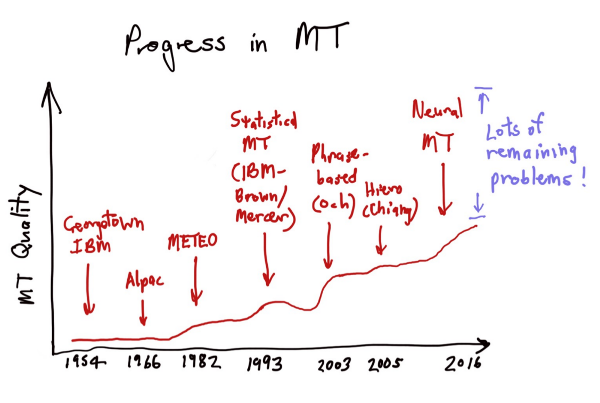
\includegraphics[width=\linewidth]{figs/intro/nmt-history.png}
%\caption{History of machine translation systems. Slide by Christopher D. Manning.}
%\end{figure}


\section{Towards Efficient Neural Machine Translation}

In spite of the success, neural systems also bring about new challenges to machine translation, in which one of the central problems is efficiency. Fundamentally, this ``inefficiency '' of NMT also comes from the deep neural networks which is why the NMT can significantly outperform other solutions. For instance, a standard \footnote{Here we refer to a hyper-parameter settings of  \texttt{t2t-base} reported in the original paper.} of the recently proposed state-of-the-art NMT model  -- the Transformer Model~\cite{vaswani2017attention} -- with a total vocabulary of about $50,000$ subwords requires to learn around $50$ million free parameters from scratch. 
Such huge number of parameters bring the efficiency issue by two aspects:
\begin{figure}[hptb]
\centering
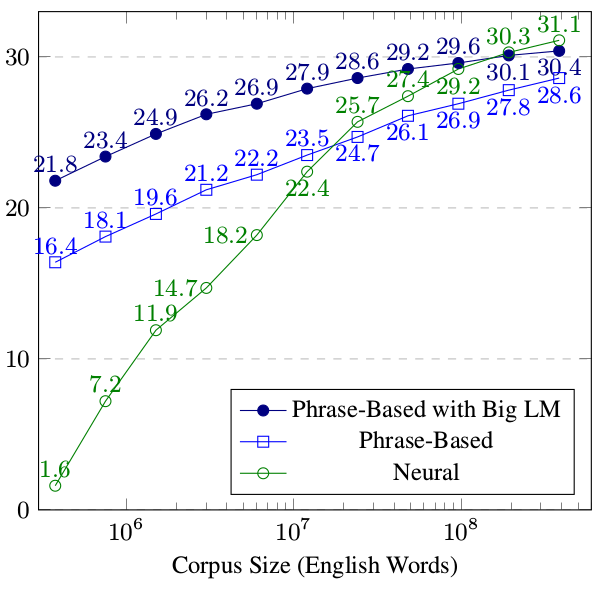
\includegraphics[width=0.6\linewidth]{figs/intro/corpus_size.png}
\caption{\label{cp1.fig.corpus_size} A comparison between NMT and SMT given varying size of training examples. Curves extracted from \newcite{koehn2017six}.}
\end{figure}
\begin{itemize}
	\item  It is significantly data-hungry to train these parameters properly using the current (and almost the only) optimization techniques via back-propagation, which makes training a reasonable model difficult in practice for many low resource cases. 
For instance, documents in specialized domains such as law or medical files usually contain tons of professional translations without sufficient examples to remember everything in the network's parameters; Moreover, except for some of the mainstream languages, e.g. English, French or Chinese, most of the human languages lack enough parallel data with other languages to learn a proper NMT model. As shown in Fig.~\ref{cp1.fig.corpus_size}, the poor data-inefficiency of the existing NMT methods compared to traditional methods is also reported as one the most important challenges; 
\item The complicated structure of NMT also makes slow computation (for both training and decoding) compared to other  conventional methods mentioned above. For example, even with the vast speeding-up by the parallelism techniques (e.g. GPUs, TPUs, etc.), because of the restriction of the model assumptions (see details in Chapter~\ref{background} and Chapter~\ref{nat}), decoding sentences by NMT is still 100 or 1000 times slower than SMT or other methods. The low efficiency at inference time profoundly affects the real-life application and the smoothness of the communication. Furthermore, in cases such as video conference or real-time conversion (e.g. see an illustration of simultaneous translation in Fig.~\ref{cp1.fig.simultaneous}), we also hope the neural system to be more efficient so that it can translate at real-time which, however, is difficult for the existing NMT models. 
\end{itemize}
\begin{figure}[hptb]
\centering
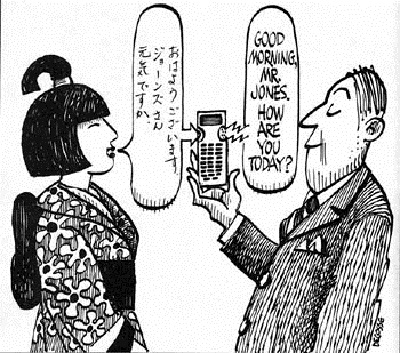
\includegraphics[width=0.6\linewidth]{figs/intro/real_time.jpg}
\caption{\label{cp1.fig.simultaneous}The goal of the efficient NMT decoding -- simultaneous translation.}
\end{figure}
For years, many research works have been taken for both cases in order to build a data and decoding efficient NMT systems. As one of the building blocks of this important trend, this dissertation will specially focus on these two directions, for each of which we claim 2-3 novel contributions to the field of machine translation research. The detailed outline of this thesis is listed below.

\section{Thesis Outline}
This dissertation attempts to tackle these two challenges discussed above, respectively, with contributions in twofold: {\it data-efficient} (Part $1$)and {\it decoding-efficient} (Part $2$) neural machine translation. 
\begin{itemize}
\item First of all, \textbf{ Chapter~\ref{background}} gives an overview for the foundation of  this dissertation,  including the modeling, training and decoding for building a general NMT model. 
\end{itemize}
For the following chapters \ref{copy}, \ref{seg-nmt}, \ref{ulr}, \ref{MetaNMT}, we address the data-efficiency challenges presented by existing NMT models and introduce insights based on the characteristics of the data.
\begin{itemize}
\item \textbf{Chapter~\ref{copy}} develops the copying mechanism as a new component  which targets on rote memories in general sequence-to-sequence (\sts) learning. The proposed \copynet also provides a general way in NMT to deal with out-of-vocabulary (OOV) words; 
\item \textbf{Chapter~\ref{seg-nmt}} uses a non-parametric search-engine to search similar translation pairs for guiding the target translation of a standard NMT system. The introduced method can be seen a direct derivation from \copynet in NMT, but forms a novel non-parametric NMT system that is able to work on translation for professional domains; 
\item \textbf{Chapter~\ref{ulr}} targets on the other direction of data-inefficiency, which invents a universal NMT system for extremely low resource languages. Different from prior works on multi-lingual translation, the proposed methods specially design two additional modules which enable a jointly-trained model works well on extremely low resource languages with around 6000 sentences; 
\item \textbf{Chapter~\ref{MetaNMT}} extends the previously proposed universal NMT system to enable a pre-trained multilingual NMT model to adapt to any new languages efficiently. Moreover, the usage of meta-learning provides a principled way of finding a better initialization of parameters that is easy to fine-tune on new languages.
\end{itemize}
For the second part with the rest of the chapters \ref{trainable}, \ref{nat} and \ref{simul}, to deal with the decoding-efficiency challenges, we develop novel structures and learning algorithms.
\begin{itemize}
\item \textbf{Chapter~\ref{trainable}} recasts the NMT decoding as a trainable process. The proposed reinforcement learning based algorithm -- {\it trainable greedy decoding} -- not only helps a trained model to decode more efficiently with greedy decoding while achieving better translation quality, but it opens an interesting direction where we can optimize the decoding towards any favorable objectives.
\item \textbf{Chapter~\ref{nat}} invents the non-autoregressive NMT system that enables translation in entirely parallel. The proposed method, with {\it fertility} as latent variables and sequence-level knowledge distillation, is one of the first NMT systems that is able to fundamentally remove the restriction of word-by-word decoding in conventional NMT models while keeping a close translation quality.
\item \textbf{Chapter~\ref{simul}} develops the NMT model that learns to translate in real-time using reinforcement learning. More precisely, we formulate the simultaneous translation as a reinforcement learning setting where two actions -- read and write -- are taken on a pre-trained normal NMT.  The resulted model successfully achieves a balance between delay and quality. 
\end{itemize}
Finally, we conclude this dissertation and discuss future avenue for efficient NMT in \textbf{Chapter~10}.	 In the next chapter, we will start to introduce in detail about the standard NMT models as the necessary background.


\chapter[Background]{Background: Neural Machine Translation}
\label{background}
In this chapter, we will introduce some background knowledge about neural machine translation on three aspects,
namely, \textit{modeling}, \textit{training}, and \textit{decoding}

\section{Modeling}
We start from discussing the building blocks that forms the most recent Neural Machine Translation (NMT) models. 
For all different architectures, NMT can always be seen as a conditional language model. 
The introduction of the attention mechanism becomes the key which enables the NMT to achieve the state-of-the-art performance.

\subsection{Neural Language Modeling}
Before discussing the details of nerual machine translation, we first come to the general topic of generating sentence using neural networks, a.k.a. neural language modeling. The research of language modeling with neural networks dates back to \citep[NNLM, ][]{bengio2003neural}  where the authors used a feed-forward network to predict next words with a fixed window size of words as input. In general, when we consider the problem of natural language modeling, a simplified view is to model languages (e.g. sentences) in a generative framework: let $V$ the vocabulary of all possible tokens, for a sentence $Y=\{y_1, y_2, ..., y_T\}$, $y_t \in V$, the language model finds a set of parameters $\theta$ to represent the reconstruction probability
$p(Y;\theta)=p(y_1, y_2, ..., y_T; \theta)$.
\paragraph{Autoregressive Language Model} Directly modeling the probability of the entire sentence $Y$ is hard and intractable. Therefore aside from some research works, most of previous efforts reformulates the probability in an autoregressive way, that is,
\begin{equation}
\label{cp2.eq.autolm}
    p(Y;\theta) = \prod_{t=1}^{T+1}p(y_t|y_{0:t-1}; \theta),
\end{equation}
where special tokens $y_0$ (e.g. $\langle \mathrm{bos}\rangle$) and $y_{T+1}$ (e.g. $\langle \mathrm{eos}\rangle$) are used to represent the beginning and end of all target sentences. The intuiative view is that the language model shows that each generated tokens $y_t$ is conditional to all previous generated tokens.
% Note that, Eq.~\ref{cp2.eq.autolm} does not require any approximation.

\paragraph{Parameterization} 
We are interested in parameterizing (approximating) these conditional probabilities using neural networks, which can be feed-forward networks, convolutional networks, or recurrent neural networks~\citep[RNNLM, ][]{mikolov2010recurrent}. 
Take the RNNLM -- a generic formulation for language model -- as an example. For each time-step $t$, the whole history $y_{0: t-1}$ is summarized as:
\begin{equation}
    \begin{split}
         h_t = f(\epsilon_I[y_{t-1}], h_{t-1}; {\theta}_f) , t \in [1, T]
    \end{split}
\end{equation}
where $\epsilon_I$ is an embedding matrix and each row maps a fixed-length vector for each input words, $f$ is the recurrent networks used to summarize the history. In practise, instead of using the vanilla RNN, RNNs with gated units are often used to capture long-term dependency in language modeling, for instance, Long-short term memory~\citep[LSTM,][]{hochreiter1997long} or Gatetd Recurrent Units~\citep[GRU,][]{cho2014learning}.
Therefore, we can compute the output probability of $y_t$ by
\begin{equation}
    \label{cp2.eq.output}
    p(y_t|y_{0: t-1};\theta) = \mathop{\softmax}\limits_{y_t\in V}\left(\epsilon_O[y_t]\cdot h_t^T\right)
\end{equation}
where $\softmax(x) = \left. {e^x} \large / {\sum_{x'} e^{x'}} \right.$ is to ensure the probabilities sum to $1$, and $\epsilon_O$ is the output weights which are sometimes tied with $\epsilon_I$. More complicated structure with multiple layers of networks can be used to enhance the modeling ability.


%These conditional probabilities are parameterized using a neural network. Typically, an encoder-decoder architecture~\citep{sutskever2014sequence} with a unidirectional RNN-based decoder is used to capture the causal structure of the output distribution.

\subsection{Sequence-to-Sequence Learning}
The neural language modeling tells how likely to a natural language sentence can be generated from nowhere, which however, is not practical in real applications. In most cases, what we are interested in is to generate meaningful sentences with certain conditions, which includes not only machine translation -- the main focus of this thsis -- but many other tasks like summarization, captioning, question answering, and response generation in dialog system. Fortunately, it is easy to borrow the experience of language modeling by assuming a conditional language modeling. 
It is also known as sequence-to-sequence ($\sts$) learning when the conditioning inputs are also sequences, e.g. neural machine translation.

\paragraph{Neural Machine Translation as \sts Learning} 
Let us denote $X=\left\{ x_1, \ldots, x_{T'} \right\}$ and $Y=\left\{ y_1, \ldots, y_T \right\}$ to denote source and target sentences in machine translation, respectively. Similar to language modeling, neural machine translation models the target sentence given the source sentence as a conditional autoregressive language model:
\begin{equation}
    p(Y|X) =  \prod_{t=1}^{T+1}p(y_t|y_{0:t-1}, x_{1:T'}; \theta),
\end{equation}
We can use the same output function as Eq.~\ref{cp2.eq.output} for each probability where in \sts learning, and the hidden states $h_t$ summarizes both the decoded and the source words
\begin{equation}
    \label{cp2.eq.hidden_state}
    \begin{split}
         h_t = f^{\textsc{dec}}(\epsilon_I[y_{t-1}], h_{t-1}, c_t(x_{1:T'}); {\theta}_f), t \in [1, T+1]
    \end{split}
\end{equation}
where $c_t(x_{1:T'})$ is the context representation of the source sentence $X$. For instance, a simple implementation proposed in \newcite{cho2014learning,sutskever2014sequence} is to use another RNN to encode the source words into a series of vector representations $s_1, ..., s_{T'}$ as 
\begin{equation}
    \label{cp2.eq.rnn_encoder}
    s_\tau = f^{\textsc{enc}}\left(\epsilon_{E}[x_\tau], s_{\tau-1}; \theta_e\right),  \tau \in [1, T']
\end{equation}
where each source word $x_\tau$ is projected into a continuous embedding space with $\epsilon_{E}$. Then, it is possible to use the last state $s_{T'}$ as the context $c$ considering it has compressed all the information we need to get the correct translation.

Borrowing the concepts from information theory, we usually call the $ f^{\textsc{enc}}$ and $ f^{\textsc{dec}}$ in \sts learning as the encoder and decoder, respectively. Intuitively in NMT, we first encode the whole source sentence $X$ into a fixed length vector $c = s_{T'}$, and then we decode the translation from it.

\begin{figure}
    \centering
    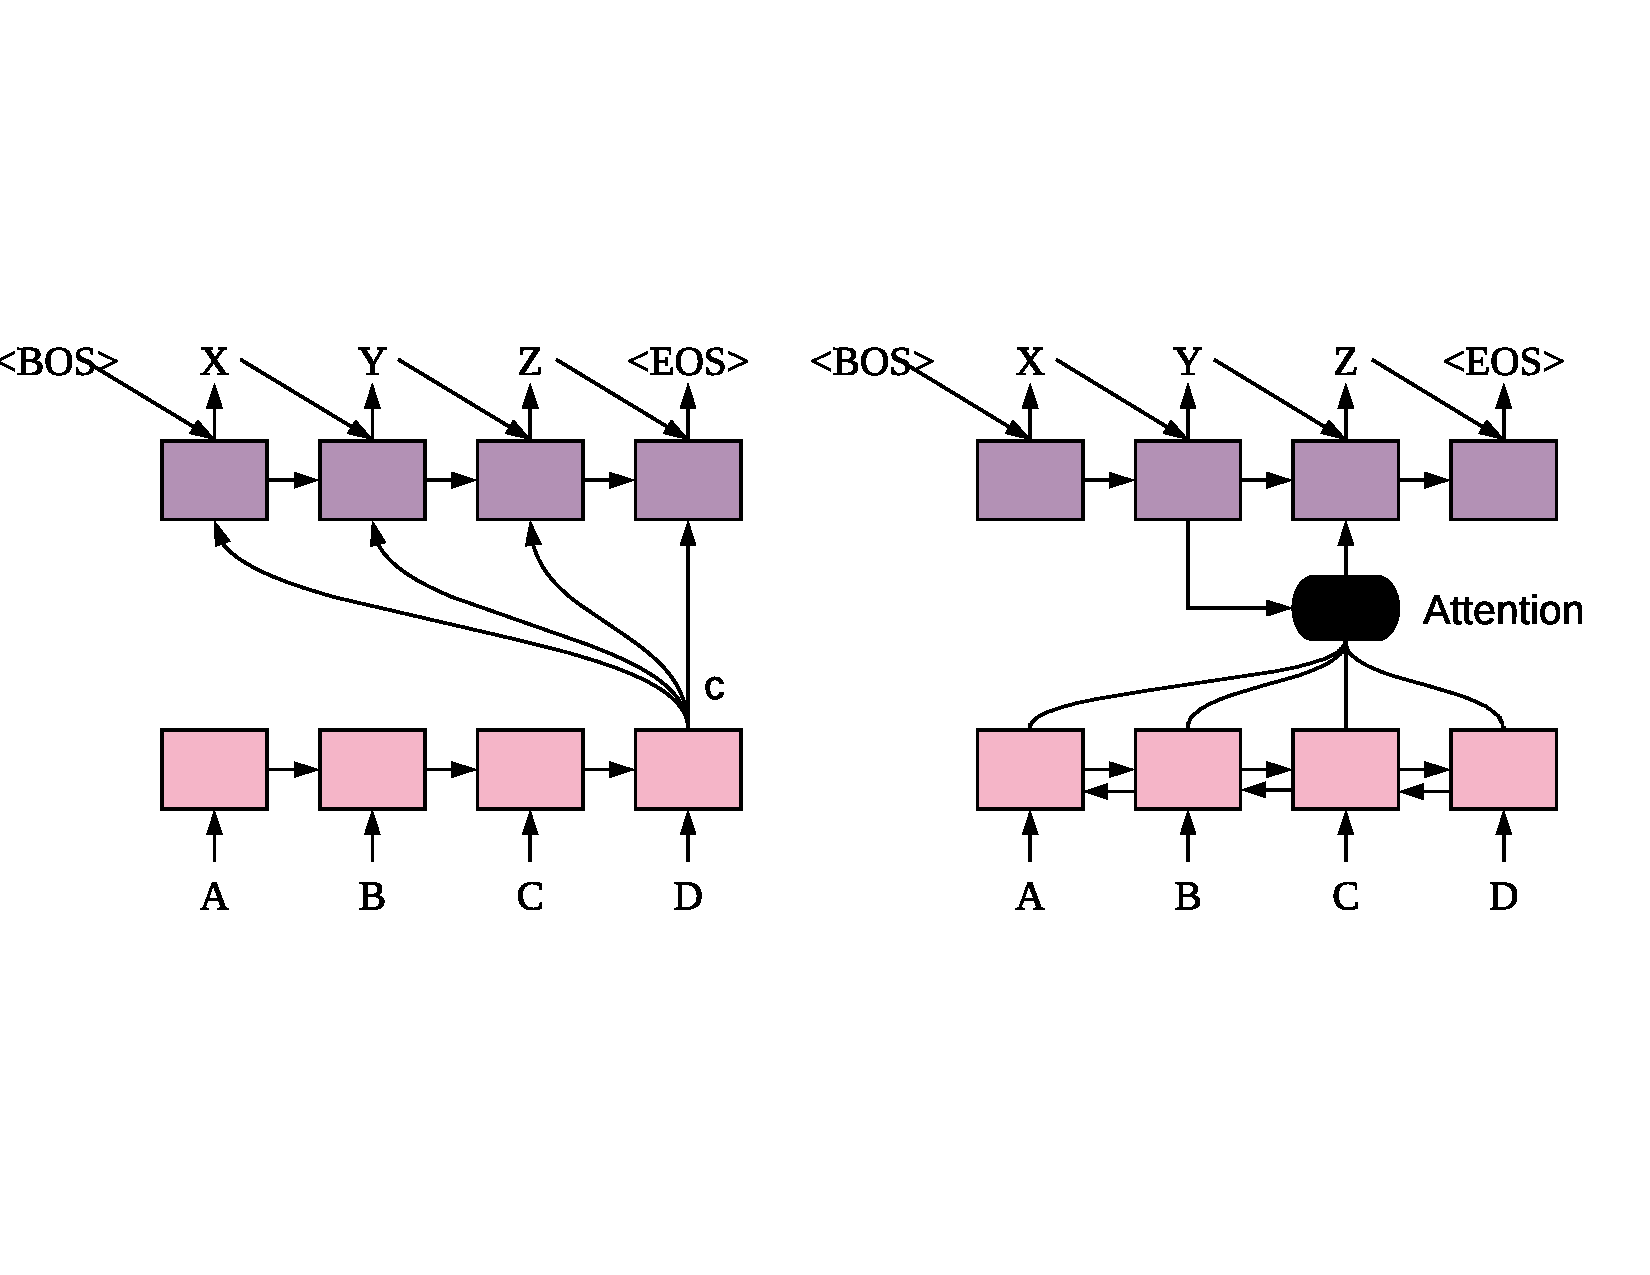
\includegraphics[width=\textwidth]{figs/background/s2s_att.pdf}
    \caption{An illustration of the comparison between the conventional \sts learning and \sts with attention mechanism for translating ``A B C D $\rightarrow$ X Y Z ''.}
    \label{cp2.fig.comparison}
\end{figure}

\subsection{Attention Mechanism}
Obviously, it is difficult to encode all the necessary information for translation into a fixed size vector, especially when the source sentence gets long. 
To release such burden, the attention mechanism was then introduced in~\newcite{bahdanau2014neural}, which was also inspired from the concept of ``alignment'' between source and target words in statistical machine translation. Instead of using a single vector for the whole decoding path, the attention mechanism uses a dynamically changing context $c_t$ in the decoding process. A natural option is to represent $c_t$ as the weighted sum of the source hidden states, i.e.
\begin{equation} 
    \label{cp2.eq.att}
	c_t = \sum_{\tau=1}^{T'}{\alpha_{t\tau} s_{\tau}}, \quad \alpha_{t\tau} =  \mathop{\softmax}\limits_\tau\left(f^{\textsc{att}}(h_{t-1}, s_{\tau}; \theta_a)\right),
\end{equation}
where $\alpha$ are the attention weights which is treated as soft-alignment, and $f^{\textsc{att}}$ is the function that shows the correspondence strength for attention, which can be either approximated with a multi-layer neural network or the inner-products between $h_{t-1}$ and $s_\tau$. 
Note that in~\newcite{bahdanau2014neural}, the source sentence is encoded with a bidirectional instead of an unidirectional RNN discussed above in Eq.~\ref{cp2.eq.rnn_encoder}, making each hidden state $s_{\tau}$ aware of the contextual information from both ends. 

The attention mechanism nicely solved the information compression problem in machine translation, and is the key for NMT to be able to achieve the state-of-the-art performance. See a comparison with a conventional \sts model in Fig.~\ref{cp2.fig.comparison}. For the following sections and chapters, without special notification, we in default consider the RNN-based \sts model with attention mechanism as the basic NMT model we used for exploration. 


\section{Training}
\subsection{Parallel Corpora}
Training requires large amount of parallel corpus

We will address this problem in the later chapters

\subsection{Maximum Likelihood Learning}
We train an NMT model, or equivalently estimate $\theta =\{\theta_f, \theta_e, \theta_a, \epsilon_E, \epsilon_I, \epsilon_O \}$, by maximizing the log-probability of the target translation $Y$ given a source sentence $X$. That is, we maximize the log-likelihood function:
\begin{equation}
    \mathcal{L}^{\text{ML}}(\theta)  = \frac{1}{N} \sum_{n=1}^N \sum_{t=1}^{T_n+1} \log p(y_t^n| y_{0:t-1}^n, x_{1:T'}^n; \theta),
\end{equation}
given a training set consisting of $N$ parallel sentence pairs. One of the fascinate things about NMT and deep learning is that, once we got the formulation of a differentiable objectives, the whole model parameters -- no matter how complex you choose your model to be -- can be trained end-to-end using stochastic gradient decent (SGD) via back-propagtation~\cite{rumelhart1986learning}. In practise, we can use modified grandients outputted from an optimizer function, such as Adadelta~\cite{zeiler2012adadelta} or Adam~\cite{kingma2014adam} to achieve a faster convergence speed and better performance .

It is important to note that this maximum likelihood learning does not take into account how a trained model would be used. Rather, it is only concerned with learning a distribution over all possible translations. 

\subsection{Advanced Learning Algorithms}
Unfortunately, MLE training has some limitations.
\citep{wiseman2016sequence,shen2015minimum,bahdanau2016actor,ranzato2015sequence}

\subsection{Multilingual Training of Neural Machine Translation}

\section{Decoding}
Once the model is trained, either by maximum likelihood learning or by any other recently proposed algorithms above, we can let the model translate a given sentence by finding a translation that maximizes 
\begin{equation}
\hat{Y} = \argmax_{Y} \log p(Y|X; \theta) =\argmax_{y_1, ..., y_T}\sum_{t=1}^{T+1} \log p(y_t| y_{0:t-1}, x_{1:T'}; \theta),
\end{equation}
where $\theta=\{\theta_f, \theta_e, \theta_a, \epsilon_E, \epsilon_I, \epsilon_O \}$, $y_0 = \langle \mathrm{bos}\rangle$ and $y_{T+1} = \langle \mathrm{eos}\rangle$. This process is so-called \textit{decoding}, which is, however, computationally intractable as the number of possible solutions grows exponentially when the decoding length $T$ increases. Although the training algorithms ensure a good approximation for the translation distribution, it does not tell how to find the translation given the distribution function. It is a usual practice to resort to approximate decoding algorithms.

\subsection{Greedy Decoding}

One such approximate decoding algorithm is greedy decoding. In greedy decoding, we follow the conditional dependency path and pick the symbol with the highest conditional probability so far at each step. This is equivalent to picking the best symbol one at a time from left to right in conditional language modeling. A decoded translation of greedy decoding is $\hat{Y} = (\hat{y}_1, \ldots, \hat{y}_T)$, where
\begin{equation}
\hat{y}_t =  \argmax_{y \in V} \log p(y|\hat{y}_{0:t-1}, x_{1:T'}; \theta).
\end{equation}
Despite its preferable computational complexity $O(|V| \times T)$, greedy decoding has been over time found to be undesirably sub-optimal.% (see, e.g., \citep{cho2016noisy}.) 

\subsection{Beam Search}  
A better option to improve the translation quality is to perform beam search.
Unlike greedy decoding which keeps only a single hypothesis, beam search keeps $K (>1)$ hypotheses simultaneously during decoding. 
That is, at each time step $t$, beam search picks $K$ hypotheses with the highest scores from the cached $K$ prefix sequences (beam)\footnote{We assume for the initial step $t=0$, we only has one symbol $\mathcal{C}_0 = \{$ \bos $\}$}:
\begin{equation}
    \mathcal{C}_{t-1} = \{\tilde{y}_{0:t-1}^{(1)}, \tilde{y}_{0:t-1}^{(2)}, ..., \tilde{y}_{0:t-1}^{(K)} \}
\end{equation}
by evaluating the cumulative conditional probabilities of all candidate hypotheses to obtain the next round of sequences: 
\begin{equation}
     \mathcal{C}_{t} = \{\tilde{y}_{0:t}^{(1)}, \tilde{y}_{0:t}^{(2)}, ..., \tilde{y}_{0:t}^{(K)} \} =
     \mathop{\argsort^K}\limits_{y_t\in V, \\  y_{0:t-1}\in \mathcal{C}_{t-1}} \sum_{t'=0}^t\log p(y_{t'}|y_{0:t'-1}, x_{1:T'}; \theta).
\end{equation}
This process repeats until one or some of the hypotheses hits the end-of-sentence symbol (\eos). Each ended sequence $\tilde{Y}$ will be selected from the cache and in the meantime, the beam size decreases $K = K - 1$.
When all hypotheses terminate, it returns the best hypothesis from the chosen sequences $\tilde{Y}_1, ..., \tilde{Y}_K$ by a re-ranking function. For instance, a simple but effective way is to use the log-probability factored by the decoding length:
\begin{equation}
    \hat{Y} = \argmax_{\tilde{Y}_1, ..., \tilde{Y}_K} \left(\frac{1}{|Y|}\right)^\alpha\cdot\log p(Y|X; \theta),
\end{equation}
where we use $|Y|$ to show the number of tokens in the decoded sentence, and $\alpha \in [0, 1]$. When we selected $\alpha=1$, the re-ranking score is equivalent to a normalized log-likelihood, or so-called perplexity. In practise, we can choose $\alpha \approx 0.6$ which can greatly help to avoid generating too short sentences.

Despite its superior performance compared to greedy decoding, the computational complexity grows linearly w.r.t. the size of beam $K$, which makes it less preferable especially in the production environment.

\subsection{Noisy Parallel Decoding}
Another alternative we can consider from is the noisy, parallel decoding (NPD) algorithm proposed in \newcite{cho2016noisy}. The main idea behind NPD algorithm is that a better translation with a higher log-probability may be found by injecting unstructured noise in the transition function of the decoder. That is,
\begin{equation}
h_t = f^{\textsc{dec}}(\epsilon_I[y_{t-1}], h_{t-1} + n_t, c_t(x_{1:T'}); \theta_f), t\in [1, T+1]
\end{equation}
where $n_t \sim \mathcal{N}(0, {\sigma_0^2} \large / {t^2})$ is the time-dependent noise. In practise, we can also other ways to inject randomness in the inner representation of the decoding process, and run greedy decoding based on the ``noisy'' inputs. 
NPD avoids potential degradation of translation quality by running such a noisy greedy decoding process multiple times in parallel. An important lesson of NPD algorithm is that there exists a decoding strategy with the asymptotically same computational complexity that results in a better translation quality, and that such a better translation can be found by manipulating the hidden state of the recurrent network. 

\section{Neural Machine Translation without RNNs}
Since the entire target translation is known at training time, the calculation of later conditional probabilities (and their corresponding losses) does not depend on the output words chosen during earlier decoding steps. 
Even though decoding must remain entirely sequential during inference, models can take advantage of this parallelism during training.
One such approach replaces recurrent layers in the decoder with masked convolution layers~\newcite{kalchbrenner2016neural, gehring2017convolutional} that provide the causal structure required by the autoregressive factorization.


\subsection{The Transformer Model}
A recently introduced option which reduces sequential computation still further is to construct the decoder layers out of self-attention computations that have been causally masked in an analogous way.
The state-of-the-art Transformer network takes this approach, which allows information to flow in the decoder across arbitrarily long distances in a constant number of operations, asymptotically fewer than required by convolutional architectures \citep{vaswani2017attention}.


% -- Sections --
% Introduction
% Bibliography
\part{Data-Efficient Neural Machine Translation}
\chapter[Copying Mechanism]{Incorporating Copying Mechanism in Sequence-to-Sequence Learning}
\label{copy}
\section{Overview}
As introduced in Chapter~\ref{background}, 
sequence-to-sequence (\sts) learning has achieved remarkable success in various natural language processing (NLP) tasks, including but not limited to  Machine Translation~\cite{cho2014learning,bahdanau2014neural}, Syntactic Parsing~\cite{vinyals2015grammar}, Text Summarization~\cite{rush2015neural} and Dialogue Systems~\cite{vinyals2015neural}. Adding the attention mechanism~\cite{bahdanau2014neural} has led to significant improvement on the performance of various tasks~\cite{shang2015neural,rush2015neural}. Different from the canonical encoder-decoder architecture, the attention-based \sts model revisits the input sequence in its raw form (array of word representations)  and dynamically fetches the relevant piece of information based mostly on the feedback from generation of the output sequence.
%on content-based addressing. 
 
In this chapter, we explore another mechanism important to the human language communication, called the ``copying mechanism", which is targeting on the data-inefficiency issue for the existing \sts learning method. Basically, it refers to the mechanism that locates a certain segment of the input sentence and puts the segment into the output sequence. For example, in the following two dialogue turns we observe different patterns in which some subsequences (colored blue) in the response (\textsf{R}) are copied from the input utterance (\textsf{I}):

\vspace{2pt}
\noindent
\begin{tabularx}{\linewidth}{@{}>{\bfseries}l@{\hspace{.4em}}X@{}}
        \toprule
    \noindent {\sf \small I:}& \texttt{\small Hello Jack, my name is {\color{blue}Chandralekha}.}\\
    \noindent {\sf \small R:}& \texttt{\small Nice to meet you, {\color{blue}Chandralekha}.}            \\
    \midrule
    \noindent {\sf \small I:} &\texttt{\small This new guy {\color{blue} doesn't perform exactly as we expected}.}\\
    \noindent {\sf \small R:} &\texttt{\small What do you mean by "{\color{blue}doesn't perform exactly as we expected}"?}\\
    \bottomrule
\end{tabularx}
 \vspace{2pt}
 
The conventional attention mechanism in \sts learning rely heavily on the representation of ``meaning'' which usually requires hundreds or thousands of examples to capture. Such ``meaning'' might not be sufficiently accurate in cases where the system needs to refer to sub-sequences of input like entity names or dates, and these words or sub-sequences may be never seen during training, for instance, out-of-vocabulary (OOV) words. 

In contrast, the copying mechanism is closer to the rote memorization in language processing of human being, 
deserving a different modeling strategy in neural network-based models. We argue that it will benefit many \sts tasks to have an elegant unified model that can accommodate both understanding and rote memorization. Towards this goal, we propose \copynet, which is not only capable of the regular generation of words but also the operation of copying appropriate segments of the input sequence. Despite the seemingly ``hard" operation of copying, \copynet can be trained in an end-to-end fashion. Our empirical study on both synthetic datasets and real world datasets demonstrates the efficacy of \copynet.       
 
 
\section{\copynet}
From a cognitive perspective, the copying mechanism is related to rote memorization, requiring less understanding but ensuring high literal fidelity. From a modeling perspective, the copying operations are more rigid and symbolic, making it more difficult than soft attention mechanism to integrate into a fully differentiable neural model.
In this section, we present \copynet, a differentiable \sts model with ``copying mechanism", which can be trained in an end-to-end fashion with standard stochastic gradient descent. 

 \begin{figure}[htbp]
   	\centering
          	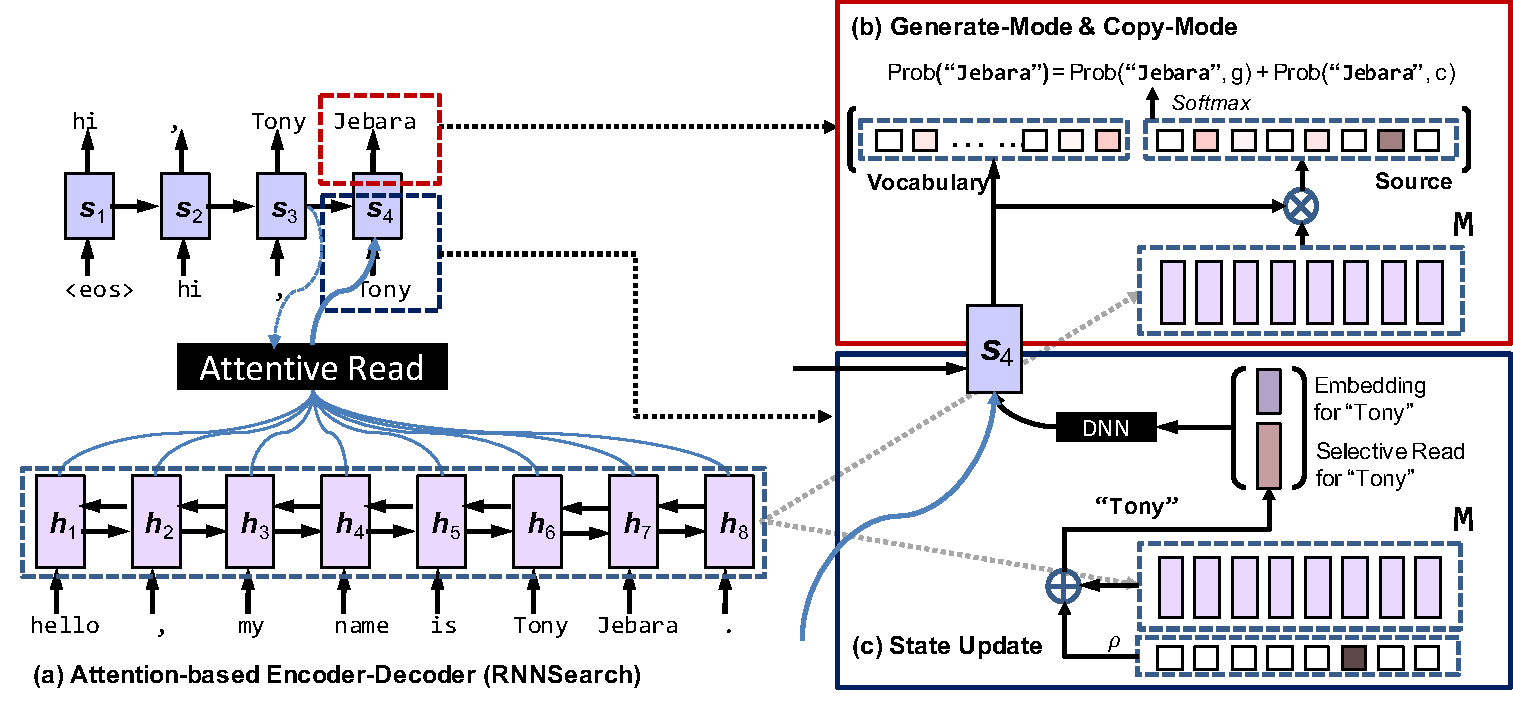
\includegraphics[width=1\linewidth]{figs/copynet/model-x.pdf} 
			  \caption{\label{cp3.fig.model} The overall diagram of \copynet. For simplicity, we omit some links for prediction. }
   \end{figure} 
   
  
\subsection{Model Overview}
As illustrated in Figure~\ref{cp3.fig.model}, \copynet is still an encoder-decoder (in a slightly generalized sense). The source sequence is transformed by \textbf{Encoder} into 
representation, which is then read by \textbf{Decoder} to generate the target sequence.

\paragraph{Encoder:} Same as in~\cite{bahdanau2014neural}, a bi-directional RNN is used to transform the source sequence into a series of hidden states with equal length, with each hidden state $h_\tau$ corresponding to word $x_\tau$. 
This new representation of the source, $\{h_1, ..., h_{T'}\}$, is considered to be a short-term memory  (referred to as $\M$ in the remainder of the paper), which will later be accessed in multiple ways in generating the target sequence (decoding).

\paragraph{Decoder:}  An RNN that reads $\M$ 
and predicts the target sequence. It is similar with the original RNN-decoder in~\cite{bahdanau2014neural}, with however the following important differences 
\begin{itemize}
    \item {\bf Prediction:}~ \copynet predicts words based on a mixed probabilistic model of two modes, namely the \textbf{generate-mode} and the \textbf{copy-mode}, where the latter picks words from the source sequence (see \S\ref{cp3.sec.predict});
	\item {\bf  State Update:}~ the predicted word at time $t-1$ is used in updating the state at $t$, but \copynet uses not only its word-embedding but also its corresponding location-specific hidden state in $\M$ (if any) (see \S\ref{cp3.sec.stateupdate} for more details);
	\item {\bf Reading $\M$:}~ in addition to the attentive read to $\M$, \copynet also has``selective read" to $\M$, which leads to a powerful hybrid of content-based addressing and location-based addressing (see both \S\ref{cp3.sec.stateupdate} and \S\ref{cp3.sec.reading} for more discussion).
\end{itemize}

\subsection{Prediction with Copying and Generation}
%\vspace{-2pt}
\label{cp3.sec.predict}
We assume a vocabulary $V=\{v_1, ..., v_M\}$, and use \unk for any out-of-vocabulary (OOV) word. 
In addition, we have another set of words $V_X$, for all the 
\emph{unique} words in source sequence $X=\{x_1, ..., x_{T'}\}$.
Since $V_X$ may contain words not in $V$, copying sub-sequence in $X$ enables 
\copynet to output some OOV words. 
In a nutshell, the instance-specific vocabulary for source $X$ is $V \cup$ \unk $\cup V_X$.

%{\color{green} \copynet predicts a word with a probabilistic model that mixes the generate-mode and the copy-mode, as illustrated in Figure~\ref{model}(b).}
Given the decoder RNN state $z_t$ at time $t$ together with $\M$,      
%the encoded source $\h(\X) = \{\mathbf{h}_1, ..., \mathbf{h}_{T_S}\}$, 
the probability of generating any target word $y_t$,  is given by the ``mixture" of probabilities as follows
\begin{equation}
p(y_t|z_t, \epsilon_I[y_{t-1}], c_t, \M; \theta) = 
p(y_t, \textsf{\small g} | z_t, \epsilon_I[y_{t-1}], c_t, \M) + 
p(y_t, \textsf{\small c}| z_t, \epsilon_I[y_{t-1}], c_t, \M) \label{cp3.eq.mix}
\end{equation}
where \textsf{\small g} stands for the generate-mode, and \textsf{\small c} the copy mode. The probability of the two modes 
are given respectively by
\begin{eqnarray} %\small 
\label{cp3.eq.pg}
p(y_t, \textsf{\small g}|\cdot) 
=&
 \left \{\begin{matrix}
\dfrac{1}{Z}e^{\psi_g(y_t)},                       \;\;\; \qquad& \;\;\; y_t \in V \\
0,                                                                          \;\;\; \qquad&\;\;\; y_t \in V_X \cap \bar{V}\\
\dfrac{1}{Z}e^{\psi_g(\textsc{unk})} \;\;\;\;     \;\;\; \qquad& \;\;\; y_t \not \in V \cup V_X     \\
\end{matrix}\right. \\
\label{cp3.eq.pc}
	p(y_t, \textsf{\small c}|\cdot)
	=& 
	\left \{\begin{matrix}
\dfrac{1}{Z}\sum_{j:x_j=y_t} e^{\psi_c(x_j)},  \hspace{-17pt} &y_t \in V_X \\
0 &\text{otherwise} 
\end{matrix}\right. 
\end{eqnarray}

%\begin{equation} %\small 
%\label{eq:pg}
%p(y_t, \textsf{\small g}|\cdot) = \left \{\begin{matrix}
%e^{\psi_g(y_t)}/Z, ~ &y_t \in \calV \\
%0,~ & y_t \in \calX \cap \bar{V}\\
%e^{\psi_g(\textsc{unk})}/Z ~ & y_t \not \in \calV \cup \calX     \\
%\end{matrix}\right.
%\end{equation}
%\begin{equation}
%\label{cp3.eq.pc}
%	p(y_t, \textsf{\small c}|\cdot)\hspace{-3pt} = \hspace{-3pt} \left \{\begin{matrix}
%\sum_{j:x_j=y_t} e^{\psi_c(x_j)}/Z,  \hspace{-7pt} &y_t \in \calX \\
%0 &\text{otherwise}  \\
%\end{matrix}\right.
%\end{equation}
where $\psi_g(\cdot)$ and $\psi_c(\cdot)$ are score functions for generate-mode and copy-mode, 
respectively, and $Z$ is the normalization term shared by the two modes, 
$Z = \sum_{v\in \cal V \cup \uunk }e^{\psi_g(v)} + \sum_{x\in X}e^{\psi_c(x)}.$
% [check the equation]. 
Due to the shared normalization term, 
the two modes are basically competing through a softmax function 
(see Figure~\ref{cp3.fig.model} for an illustration with example), 
rendering Eq.~\eqref{cp3.eq.mix} deviated from the canonical definition of mixture model~\cite{GaussianMixture}. This is also pictorially illustrated in Figure \ref{cp3.fig.oov}. 
 The score of each mode is calculated:
\paragraph{Generate-Mode:}~The same scoring function as in the generic RNN encoder-decoder~\cite{bahdanau2014neural} is used, i.e.
\begin{equation}\label{cp3.eq.gen}
	\psi_g(y_t=v_i) = \epsilon_O[v_i]^\top \cdot z_t, \quad v_i \in V \cup \uunk, 
\end{equation}
where $\epsilon_O \in \mathbb{R}^{(M+1) \times d_s}$. 

\paragraph{Copy-Mode:}~The score for ``copying" the word $x_j$ is calculated as 
\begin{equation}\label{cp3.eq.cp}
	\psi_c(y_t=x_j) = \sigma\left(h_j^\top \epsilon_C \right)\cdot z_t, \quad  x_j \in V_X,
\end{equation}
where $\epsilon_C \in \mathbb{R}^{d_h \times d_s}$, and $\sigma$ is a non-linear activation function, considering that the non-linear transformation in Eq~\eqref{cp3.eq.cp} can help project $h_t$ and $z_j$ in the same semantic space. Empirically,  we also found that using the $\tanh$ non-linearity worked better than linear transformation, and we used that for the following experiments.
When calculating the copy-mode score, we use the hidden states $\{ h_1, ..., h_{T'} \} $ to ``represent" each of the word in the source sequence $\{x_1, ..., x_{T_S}\}$ since the bi-directional RNN encodes not only the content, 
but also the location information into the hidden states in $\M$. The location informaton is important for copying (see \S\ref{cp3.sec.reading} for related discussion). 
Note that we sum the probabilities of all $x_j$ equal to $y_t$ in Eq.~\eqref{cp3.eq.pc} considering that there may be multiple source symbols for decoding $y_t$. 
%\vspace{-5pt}
% where $y \in X \cup V \cup \{v_{\text{unk}}\}$ regarding all the symbols outside $X \cup V$ as the same symbol ``unk".
\begin{figure}[htpb]
   	\centering
          	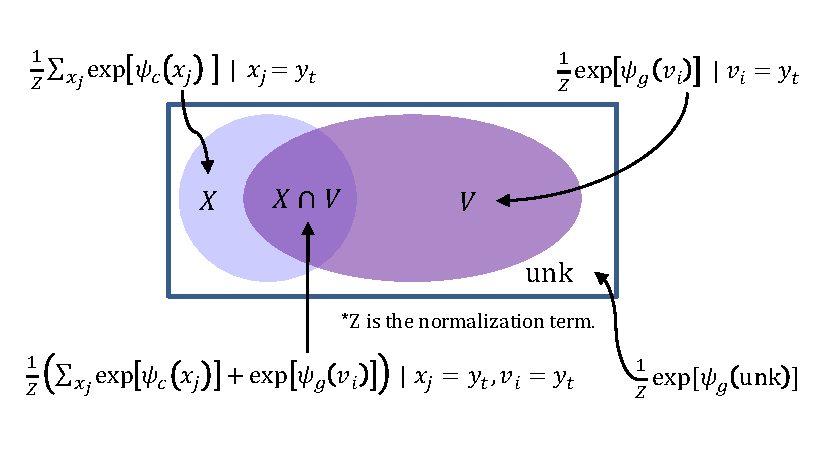
\includegraphics[width=0.85\linewidth]{figs/copynet/oov.pdf} 
          	\caption{\label{cp3.fig.oov} The illustration of  the decoding probability $p(y_t|\cdot)$
          	 %which is seen 
          	 as a 4-class classifier. } 
  \end{figure}   
Naturally we let $p(y_t, \textsf{\small c}|\cdot)=0$ if $y_t$ does not appear in the source sequence, 
and set $p(y_t, \textsf{\small g}|\cdot)=0$ when $y_t$ only appears in the source. %Such changes make the probabilities sum up to 1.% and shrinks the range of the OOV words.

 \subsection{State Update}
\label{cp3.sec.stateupdate}
\copynet updates each decoding state $z_{t}$ with the previous state $z_{t-1}$, 
the previous symbol $y_{t-1}$ and the context vector $c_{t}$ 
for the generic attention-based \sts model. 
However, there is some minor changes in the 
$y_{t-1}\longrightarrow z_{t}$ path for the copying mechanism. 
More specifically, $y_{t-1}$ will be represented as $\left[\epsilon_I[y_{t-1}] ; \zeta(y_{t-1})\right]^\top$, 
while $\zeta(y_{t-1})$ is the weighted sum of hidden states in $\M$ corresponding to $y_t$ 
\begin{equation}
%\small
\label{cp3.eq.loc}
\begin{split}
%	&\zeta(y_{t-1}) = \left \{ \begin{matrix}
%		\sum\nolimits_{\tau=1}^{T_S}\rho_{t\tau} \h_{\tau} \quad & y_{t-1} \in \calX\\
%		\textbf{0} \quad & \text{otherwise} 
%	\end{matrix}\right.
	&\zeta(y_{t-1}) = \sum\nolimits_{\tau=1}^{T'}\rho_{t\tau} h_{\tau}\\
	&\rho_{t\tau} = \left \{ \begin{matrix} 
	     \dfrac{1}{K} p(x_\tau, \textsf{c} | z_{t-1}, \M),
	    %\dfrac{p(x_\tau, c | \sss_{t-1}, \h)}{\sum\nolimits_{\tau':x_{\tau'}=y_{t-1}} p(x_\tau', c | \sss_{t-1}, \h)}
	     \quad & x_{\tau} = y_{t-1}\\
		0 \quad & \text{otherwise} 
	\end{matrix}\right.
%	&\rho_{t\tau} = \text{Nor}\left[ p(x_\tau, c | \cdot) \odot \mathds{1}(y_{t-1} - x_{\tau})\right]\\
%	&\rho_{t\tau} = \hat{\rho}_{t\tau}/{\sum\nolimits_{\tau'}\hat{\rho}_{t\tau'}};  \hat{\rho}_{t\tau} = P(x_\tau) \cdot (y_t == x_{\tau})
\end{split} 
\end{equation}
where $K$ is the normalization term 
which equals $\sum_{{\tau'}:x_{\tau'}=y_{t-1}} p(x_{\tau'}, c | z_{t-1}, \M)$, 
considering there may exist multiple positions with $y_{t-1}$ in the source sequence. 
In practice, $\rho_{t\tau}$ is often concentrated on one location among multiple appearances, 
indicating the prediction is closely bounded to the location of words.  

In a sense $\zeta(y_{t-1})$ performs a type of read to $\M$ similar to 
the attentive read (resulting $c_t$) with however higher precision. 
In the remainder of this chapter, $\zeta(y_{t-1})$ will be referred to as \emph{selective read}. 
$\zeta(y_{t-1})$ is specifically designed for the copy mode: 
with its pinpointing precision to the corresponding  $y_{t-1}$, 
it naturally bears the location of $y_{t-1}$ in the source sequence encoded in the hidden state. 
As will be discussed more in \S\ref{cp3.sec.reading}, 
this particular design potentially helps copy-mode in covering a consecutive sub-sequence of words. 
If $y_{t-1}$ is not in the source,  we let $\zeta(y_{t-1})=\textbf{0}$. 


%{\color{blue} In this paper $\zeta(y_{t-1})$ is named \emph{selective read}, since it can be viewed as another kind of read from the $\M$ when it fetches the hidden state for decoder. Different from attentive read, selective read at time $t$ is determined jointly by $y_{t}$ and $\sss_t$, which in practice is usually concentrated into one particular hidden state even if the word $y_{t}$ has multiple appearances in the source.
%}
 %Concatenating with the content-based input, we 
 
%{\color{blue} 
%The location-based input can be explained intuitively that in many tasks, we perform ``copy and paste" focusing more on the locations of the segments rather than the detailed content behind the them. Each segment typically consists of successive symbols, and it will be helpful to input the previous location to move on the target position. 
%}

\subsection{Hybrid Addressing of Short-Term Memory} 
\label{cp3.sec.reading}
We hypothesize that \copynet uses a hybrid strategy for fetching the content in $\M$, 
which combines both content-based and location-based addressing. 
Both addressing strategies are coordinated by the decoder in managing the attentive read and selective read, 
as well as determining when to enter/quit the copy-mode. 

Both the semantics of a word and its location in $X$ will be encoded into the hidden states in $\M$ by a properly trained encoder. 
Judging from our experiments, the attentive read of \copynet is driven more by the semantics and language model, 
therefore capable of traveling more freely on $\M$, even across a long distance. 
On the other hand, once \copynet enters the copy-mode, the selective read of $\M$ is often guided by the location information. 
As the result, the selective read often takes rigid move and tends to cover consecutive words, including \unk.  
Unlike the explicit design for hybrid addressing in Neural Turing Machine~\cite{graves2014neural,kurach2015neural}, 
\copynet is more subtle: it provides the architecture that can facilitate some particular location-based addressing and 
lets the model figure out the details from the training data for specific tasks. 

\paragraph{Location-based Addressing} 
With the location information in $\{ h_i \} $, the information flow %(need to define earlier) 
\[
%\cdots \rightarrow
\zeta(y_{t-1}) \xrightarrow{\text{update}}  z_{t} \xrightarrow{\text{predict}} y_{t} \xrightarrow{\text{sel. read}}  \zeta(y_{t}) 
%\rightarrow \cdots 
\]
provides a simple way of ``moving one step to the right" on $X$. 
More specifically, assuming the selective read $\zeta(y_{t-1})$ concentrates on the $\ell^{th}$ word in $X$, 
the state-update operation $\zeta(y_{t-1})\hspace{-4pt} \xrightarrow{\text{update}} \hspace{-4pt} h_t $ acts as 
``\texttt{\small location} $\leftarrow$ \texttt{\small location+1}", 
making $z_t$ favor the $(\ell \hspace{-3pt}+\hspace{-3pt}1)^{th}$ word in $X$ in the prediction 
$z_t \xrightarrow{\text{predict}} y_{t}$ in copy-mode. 
This again leads to the selective read  $z_{t} \hspace{-3pt}\xrightarrow{\text{sel. read}} \hspace{-3pt} \zeta(y_{t})$ 
for the state update of the next round.

\paragraph{Handling Out-of-Vocabulary Words}
Although it is hard to verify the exact addressing strategy as above directly, 
there is strong evidence from our empirical study. 
Most saliently, a properly trained \copynet can copy a fairly long segment full of OOV words, 
despite the lack of semantic information in its $\M$ representation. 
This provides a natural way to extend the effective vocabulary to include all the words in the source. 
Although this change is small, it seems quite significant empirically in alleviating the OOV problem. 
Indeed, for many NLP applications (e.g., text summarization or spoken dialogue system),  
much of the OOV words on the target side, for example the proper nouns, 
are essentially the replicates of those on the source side.

\section{Learning} 	
Although the copying mechanism uses the ``hard" operation to copy from the source and choose to paste them or generate symbols from the vocabulary, \copynet is fully differentiable and can be optimized in an end-to-end fashion using maximum likelihood learning which was previously introduced in 	Chapter~\ref{background} as Eq.~\eqref{cp2.eq.learning}.
%Given the batches of the source and target sequence $\{X\}_N$ and $\{Y\}_N$, the objectives are to minimize the negative log-likelihood:
%	\begin{equation}
%      \mathcal{L} = -\frac{1}{N}\sum_{k=1}^N\sum_{t=1}^{T}\log \left[ p(y^{(k)}_t|y^{(k)}_{<t}, X^{(k)})\right], 	\vspace{-9pt}
%%     \mathcal{L} = -\frac{1}{N}\sum_{k=1}^N\sum_{t=1}^{T}\log \left[ P(y^{(k)}_t, g|\cdot) + P(y^{(k)}_t, c|\cdot)\right]
%\end{equation}

 Since the probabilistic model for observing any target word is a mixture of generate-mode and copy-mode, there is no need for any additional labels for modes. The network can learn to coordinate the two modes from data. More specifically, if one particular word $y_{t}$ can be found in the source sequence, the copy-mode will contribute to the mixture model, and the gradient will more or less encourage the copy-mode; otherwise, the copy-mode is discouraged due to the competition from the shared normalization term $Z$. In practice, in most cases one mode dominates.


\section{Experiments}
We report our empirical study of \copynet on the following three tasks with different characteristics
\begin{enumerate}
	%\vspace{-7pt}
	\item A synthetic dataset on with simple patterns;
	%\vspace{-7pt}
	\item A real-world task on text summarization;
	%\vspace{-7pt}
	\item A dataset for simple single-turn dialogues.
\end{enumerate}  

\subsection{Synthetic Dataset}
\label{cp3.sec.synthetic}
\textbf{Dataset:}~  
We first randomly generate transformation rules with 5$\sim$20 symbols and variables $\mathbf{x}$ \& $\mathbf{y}$, e.g.   
\[
\texttt{a b } \mathbf{x} \texttt{ c d }\mathbf{y} \texttt{ e f} \longrightarrow \texttt{ g h }\mathbf{x}\texttt{ m},  
%\vspace{-5pt}
\]
with \{\texttt{a\;b\;c\;d\;e\;f\;g\;h\;m}\} being regular symbols from a vocabulary of size 1,000. As shown in the table below, each rule can further produce a number of instances by replacing the variables with randomly generated subsequences (1$\sim$15 symbols) from the same vocabulary. We create five types of rules, including ``$\mathbf{x}\rightarrow$ $\emptyset$".
The task is to learn to do the \sts transformation from the training instances. 
This dataset is designed to study the behavior of \copynet on handling simple and rigid patterns. Since the string to repeat are random, they can also be viewed as some extreme cases of rote memorization.   
%{\color{red}This dataset is designed to demonstrate the clear mechanism of \copynet. }
%, instances generated are designed to evaluate the copying mechanism in each situation.
% We create the synthetic dataset named ``Simple Rules for \textsc{Seq2seq} Learning (SRSS)" for this analysis.  
%The dataset contains different symbols with a vocabulary of 1,000 words (with indices from $0$ to $999$) and two variables \textbf{X} \& \textbf{Y}.  
%%%%%%%%%%%%%%%%%%%%%%%%%%%%%%%%%%%%%%%%%%%%%%%%
 \begin{table}[htpb] % "[h!]" location specifier just for this example
\centering
\begin{tabular}{l|l}
\toprule
 Rule-type& {Examples (e.g. $\mathbf{x}$ = $\texttt{i h k}$,~~ $\mathbf{y}$ = $\texttt{j c}$)} \\
\midrule
$\mathbf{x}$ $\rightarrow \emptyset$ 
& $\texttt{a b c d }\mathbf{x} \texttt{ e f} \rightarrow \texttt{c d g}$\\
\cmidrule{1-2}
$\mathbf{x}$ $\rightarrow$ $\mathbf{x}$ 
& $\texttt{a b c d }\mathbf{x} \texttt{ e f} \rightarrow \texttt{c d } \mathbf{x} \texttt{ g} $\\
$\mathbf{x}$ $\rightarrow$ $\mathbf{x\,x}$ 
& $\texttt{a b c d }\mathbf{x} \texttt{ e f} \rightarrow \mathbf{x}  \texttt{ d } \mathbf{x} \texttt{ g} $\\
$\mathbf{x\,y}$ $\rightarrow$ $\mathbf{x}$ 
& $\texttt{a b } \mathbf{y} \texttt{ d }\mathbf{x} \texttt{ e f} \rightarrow \mathbf{x}  \texttt{ d i g} $\\
$\mathbf{x\,y}$ $\rightarrow$ $\mathbf{x\,y}$ 
& $\texttt{a b } \mathbf{y} \texttt{ d }\mathbf{x} \texttt{ e f} \rightarrow \mathbf{x}  \texttt{ d } \mathbf{y} \texttt{ g} $\\
\bottomrule
\end{tabular}
\caption{\label{cp3.table.syn_exp} Examples of synthetic rules and examples}
\end{table} 

\paragraph{Experimental Setting} We select 200 artificial rules from the dataset, and for each rule 200 instances are generated, which will be split into training (50\%) and testing (50\%).  We compare the  accuracy of \copynet and the RNN Encoder-Decoder with (denoted as RNNsearch) or without attention (denoted as Enc-Dec).
For a fair comparison, we use bi-directional GRU~\cite{cho2014learning} for encoder and another GRU for decoder  for all the models, with hidden layer size = 300 and word embedding dimension = 150. We use beam size  $=10$ in beam search for testing. The prediction is considered correct only when the generated sequence is exactly the same as the given one. 
%It is clear that the system must make full use of the limited instances to summarize patterns and then output the results correctly.
%\\ \vspace{-7pt} \\

%We compare the accuracy of \copynet and the baseline RNNSearch. It is clear from Table~\ref{cp3.table.acc} that \copynet significantly outperforms RNNsearch on all rule-types except ``$\mathbf{x} \rightarrow \emptyset$", indicating that \copynet can effectively learn the patterns from instances and accurately repeat rather long subsequence of symbols at the proper places. {\color{blue} This is often hard to an canonical encoder-decoder framework due to the difficulty of representing a long sequence with very high fidelity. This difficulty can be alleviated with the attention mechanism,

%{\color{red}but ...  A closer look at \copynet trained on this data set reveals that ... }
%%%%%%%%%%%%%%%%%%%%%%%%%%%%%%%%%%%%%%%%%%%%%%%%
 \begin{table}[hptb] % "[h!]" location specifier just for this example
\centering
\begin{tabular}{lccccc}
\toprule
Rule-type& $\mathbf{x}$ &  $\mathbf{x}$ &   $\mathbf{x}$ &   $\mathbf{xy}$&    $\mathbf{xy}$ \\% & Avg. \\
&  $\rightarrow \emptyset$ &  $\rightarrow\mathbf{x}$ &  $\rightarrow\mathbf{xx}$ &  $\rightarrow\mathbf{x}$&   $\rightarrow\mathbf{xy}$  \\
\midrule
%RNNEncDec
%& 110  &&&&& \\
%\cmidrule{1-2}
Enc-Dec
& \textbf{100}  & 3.3 & 1.5 & 2.9 & 0.0\\
RNNSearch 
& 99.0  & 69.4 & 22.3 & 40.7 & 2.6\\
\midrule
\copynet
& 97.3  & \textbf{93.7} & \textbf{98.3} & \textbf{68.2} & \textbf{77.5}\\
\bottomrule
\end{tabular} 
\caption{\label{cp3.table.acc}  The test accuracy (\%) on synthetic data.}
%The decoding accuracy in percentage on the testing set with different rule-types.} % Three kinds of instances are evaluated for our model: from top to bottom are (a) repeated  (b) ordered, and (c) random, respectively.}
\end{table} %\vspace{-15pt}

It is clear from Table~\ref{cp3.table.acc} that \copynet significantly outperforms the other two on all rule-types except ``$\mathbf{x} \rightarrow \emptyset$", indicating that \copynet can effectively learn the patterns with variables and accurately replicate rather long subsequence of symbols at the proper places.This is hard to Enc-Dec due to the difficulty of representing a long sequence with very high fidelity. This difficulty can be alleviated with the attention mechanism. However attention alone seems inadequate for handling the case where strict replication is needed. 

A closer look (see Figure~\ref{cp3.fig.syn} for example) reveals that the decoder is dominated by copy-mode when moving into the subsequence to replicate, and switch to generate-mode after leaving this area, showing \copynet can achieve a rather precise coordination of the two modes. \vspace{-5pt}    
\begin{figure}[hptb]
   	\centering
          	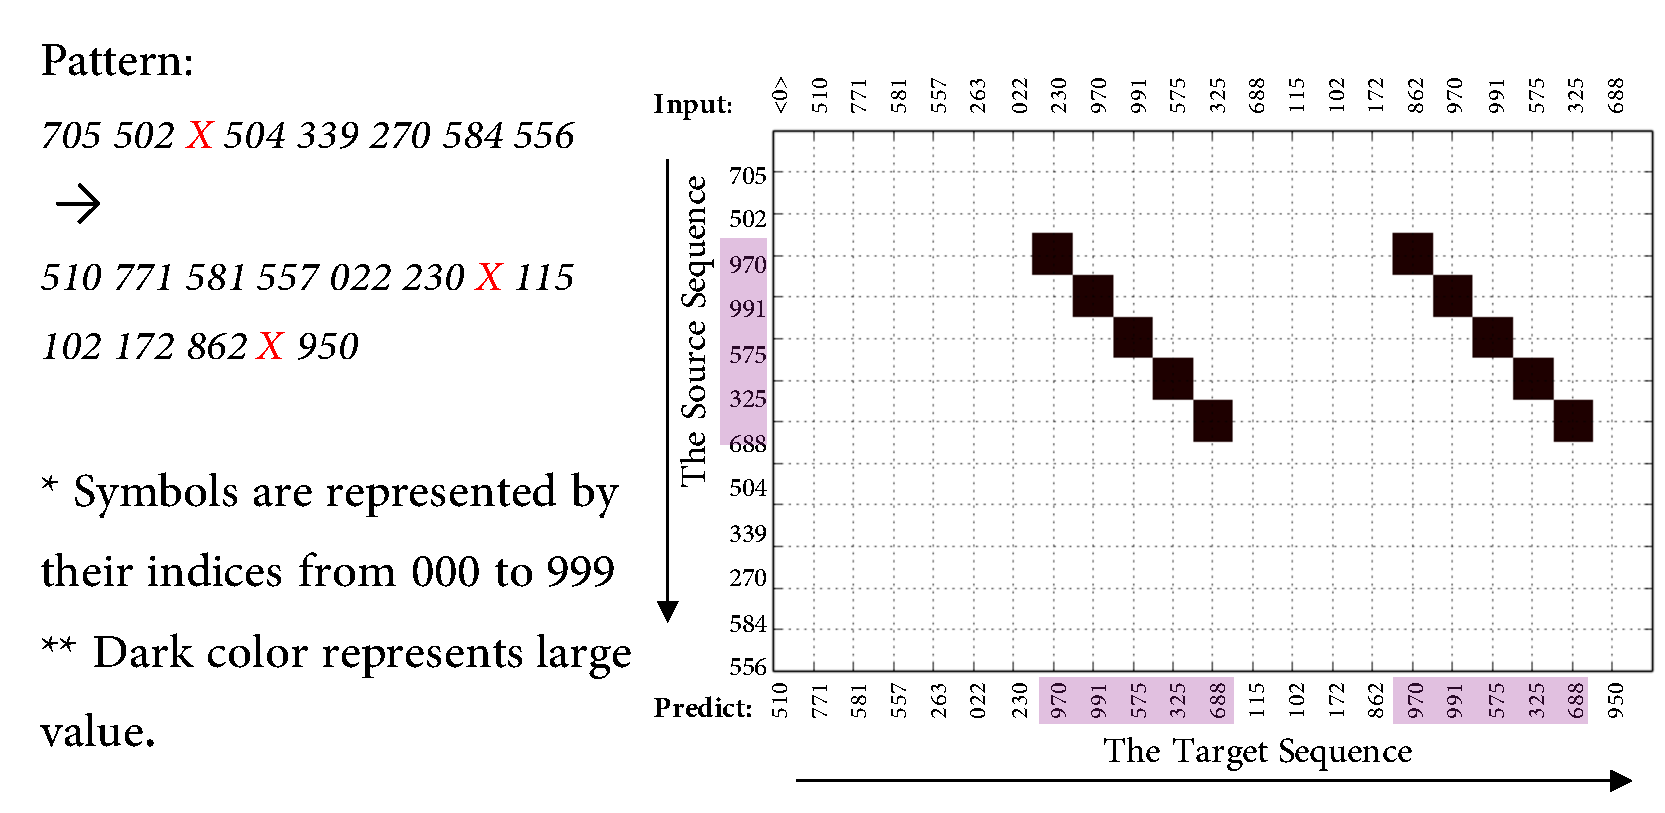
\includegraphics[width=.98\linewidth]{figs/copynet/syn2.pdf} 
          	\caption{\label{cp3.fig.syn} Example output of \copynet on the synthetic dataset. The heatmap represents the activations of the copy-mode over the input sequence (left) during the decoding process (bottom).} 
  \end{figure}   

\subsection{Text Summarization}
Automatic text summarization aims to find a condensed representation which can capture the core meaning of the original document. It has been recently formulated as a \sts learning problem in~\cite{rush2015neural,hu2015lcsts}, which essentially gives \emph{abstractive} summarization since the summary is generated based on a representation of the document. In contrast, \textit{extractive} summarization extracts sentences or phrases from the original text to fuse them into the summaries, therefore making better use of the overall structure of the original document. In a sense, \copynet for summarization lies somewhere between two categories, since part of output summary is actually extracted from the document (via the copying mechanism), which are fused together possibly with the words from the generate-mode.


%%As mentioned above,  encoder-decoder models easily come across the problems of OOVs when doing summarization. 
%However,
%%have to encode the whole input text for ``understanding" their meanings implicitly to generate a summary, which sometimes is not essential and comes across the problem of OOVs. 
%on the perspectives of  \copynet,  its generate and copy modes just correspond to the \textit{abstractive} and \textit{extractive} behaviours in summarization, respectively. \\ \vspace{-7pt} \\
\paragraph{Dataset}~We evaluate our model on LCSTS dataset~\cite{hu2015lcsts},  a large scale dataset for short text summarization. The dataset is collected from the news medias on Sina Weibo\footnote{www.sina.com} including pairs of (short news, summary) in Chinese. Shown in Table~\ref{cp3.table.lcsts},  PART \uppercase\expandafter{\romannumeral2}  and  \uppercase\expandafter{\romannumeral3} are manually rated for their quality from 1 to 5. Following~\cite{hu2015lcsts}, we use Part \uppercase\expandafter{\romannumeral1}  as the training set and and the subset of Part  \uppercase\expandafter{\romannumeral3} scored from 3 to 5 as testing set. 

  %%%%%%%%%%%%%%%%%%%%%%%%%%%%%%%%%%%%%%%%%%%%%%%%
\begin{table}[hptb] % "[h!]" location specifier just for this example
\centering
\begin{tabular}{l|ccc}
\toprule
Dataset & PART \uppercase\expandafter{\romannumeral1}  & PART \uppercase\expandafter{\romannumeral2}  & PART \uppercase\expandafter{\romannumeral3} \\
\midrule
no. of pairs & 2,400,591  &  10,666 & 1106\\
no. of $\text{score} \geq 3$ & - & 8685 & 725 \\
\bottomrule
\end{tabular} 
\caption{\label{cp3.table.lcsts} The statistics of the LCSTS dataset.} % Three kinds of instances are evaluated for our model: from top to bottom are (a) repeated  (b) ordered, and (c) random, respectively.}
\end{table}

\paragraph{Experimental Setting}~We try \copynet that is based on character (+C) and word (+W). For the word-based variant the word-segmentation is obtained with jieba\footnote{https://pypi.python.org/pypi/jieba}. We set the vocabulary size to 3,000 (+C) and 10,000 (+W) respectively, which are much smaller than those for models in~\cite{hu2015lcsts}. For both variants we set the embedding dimension to 350 and the size of hidden layers to 500. %\\ \vspace{-7pt} \\
%\copynet is optimized on the training set through Adam~\cite{kingma2014adam} using a batch size of 20. 
We evaluate the test performance with the commonly used ROUGE-1, ROUGE-2 and ROUGE-L~\cite{lin:2004:ACLsummarization}, and compare it against the two models in \cite{hu2015lcsts}, which are essentially canonical Encoder-Decoder and its variant with attention.  
 %%%%%%%%%%%%%%%%%%%%%%%%%%%%%%%%%%%%%%%%%%%%%%%%
%We need to generate synthetic sequences with suitable patterns for \textsc{Seq2seq} learning.
 \begin{table}[htb] % "[h!]" location specifier just for this example
%\vspace{-20pt}
\centering
\begin{tabular}{llccc}
\toprule
 Models&& \multicolumn{3}{c}{ROUGE scores on LCSTS (\%)} \\
%\cmidrule{2-3}
 && R-1 &\hspace{14pt} R-2 & R-L	\\
\midrule
RNN &  +C  & 21.5 & \hspace{14pt}8.9 & 18.6 \\
\cite{hu2015lcsts} & +W & 17.7 & \hspace{14pt}8.5 & 15.8 \\
%\cmidrule{3-5}
RNN context   &  +C & 29.9 & \hspace{14pt}17.4 & 27.2 \\
\cite{hu2015lcsts} & +W & 26.8 & \hspace{14pt}16.1 & 24.1 \\
%\cmidrule{3-5}
\midrule
\multirow{2}{*}{\copynet}& +C & \textbf{34.4} & \hspace{14pt}\textbf{21.6} & \textbf{31.3} \\
												    & +W & \textbf{35.0} & \hspace{14pt}\textbf{22.3} & \textbf{32.0} \\												  
\bottomrule
\end{tabular} 
\caption{\label{cp3.table.summary} Testing performance of LCSTS, where ``RNN" is canonical Enc-Dec, and ``RNN context" its attentive variant.}
\end{table} 
% \begin{table}[!ht] % "[h!]" location specifier just for this example
%\small
%\centering
%\begin{tabular}{lcccccc}
%\toprule
% Models& \multicolumn{6}{c}{LCSTS} \\
%%\cmidrule{2-3}
%& \multicolumn{2}{c}{ROUGE-1}  &\multicolumn{2}{c}{ROUGE-2} &\multicolumn{2}{c}{ROUGE-L}	\\
%\midrule
%EncDec & 10.11 & 10.11 & 10.11& 10.11 & 10.11 & 10.11 \\
%\bottomrule
%\end{tabular} \vspace{-5pt}
%\caption{\label{table-exp} Evaluation results.}
%\end{table} \vspace{-7pt}
%%%%%%%%%%%%%%%%%%%%%%%%%%%%%%%%%%%%%%%%%%%%%%%%%


It is clear from Table~\ref{cp3.table.summary} that \copynet beats the competitor models with big margin. \newcite{hu2015lcsts} reports that the performance of a word-based model is inferior to a character-based one. One possible explanation is that a word-based model, even with a much larger vocabulary (50,000 words in \newcite{hu2015lcsts}), still has a large proportion of OOVs due to the large number of entity names in the summary data and the mistakes in word segmentation. \copynet, with its ability to handle the OOV words with the copying mechanism, performs however slightly better with the word-based variant.

 \begin{figure}[htpb]
   	\centering
          	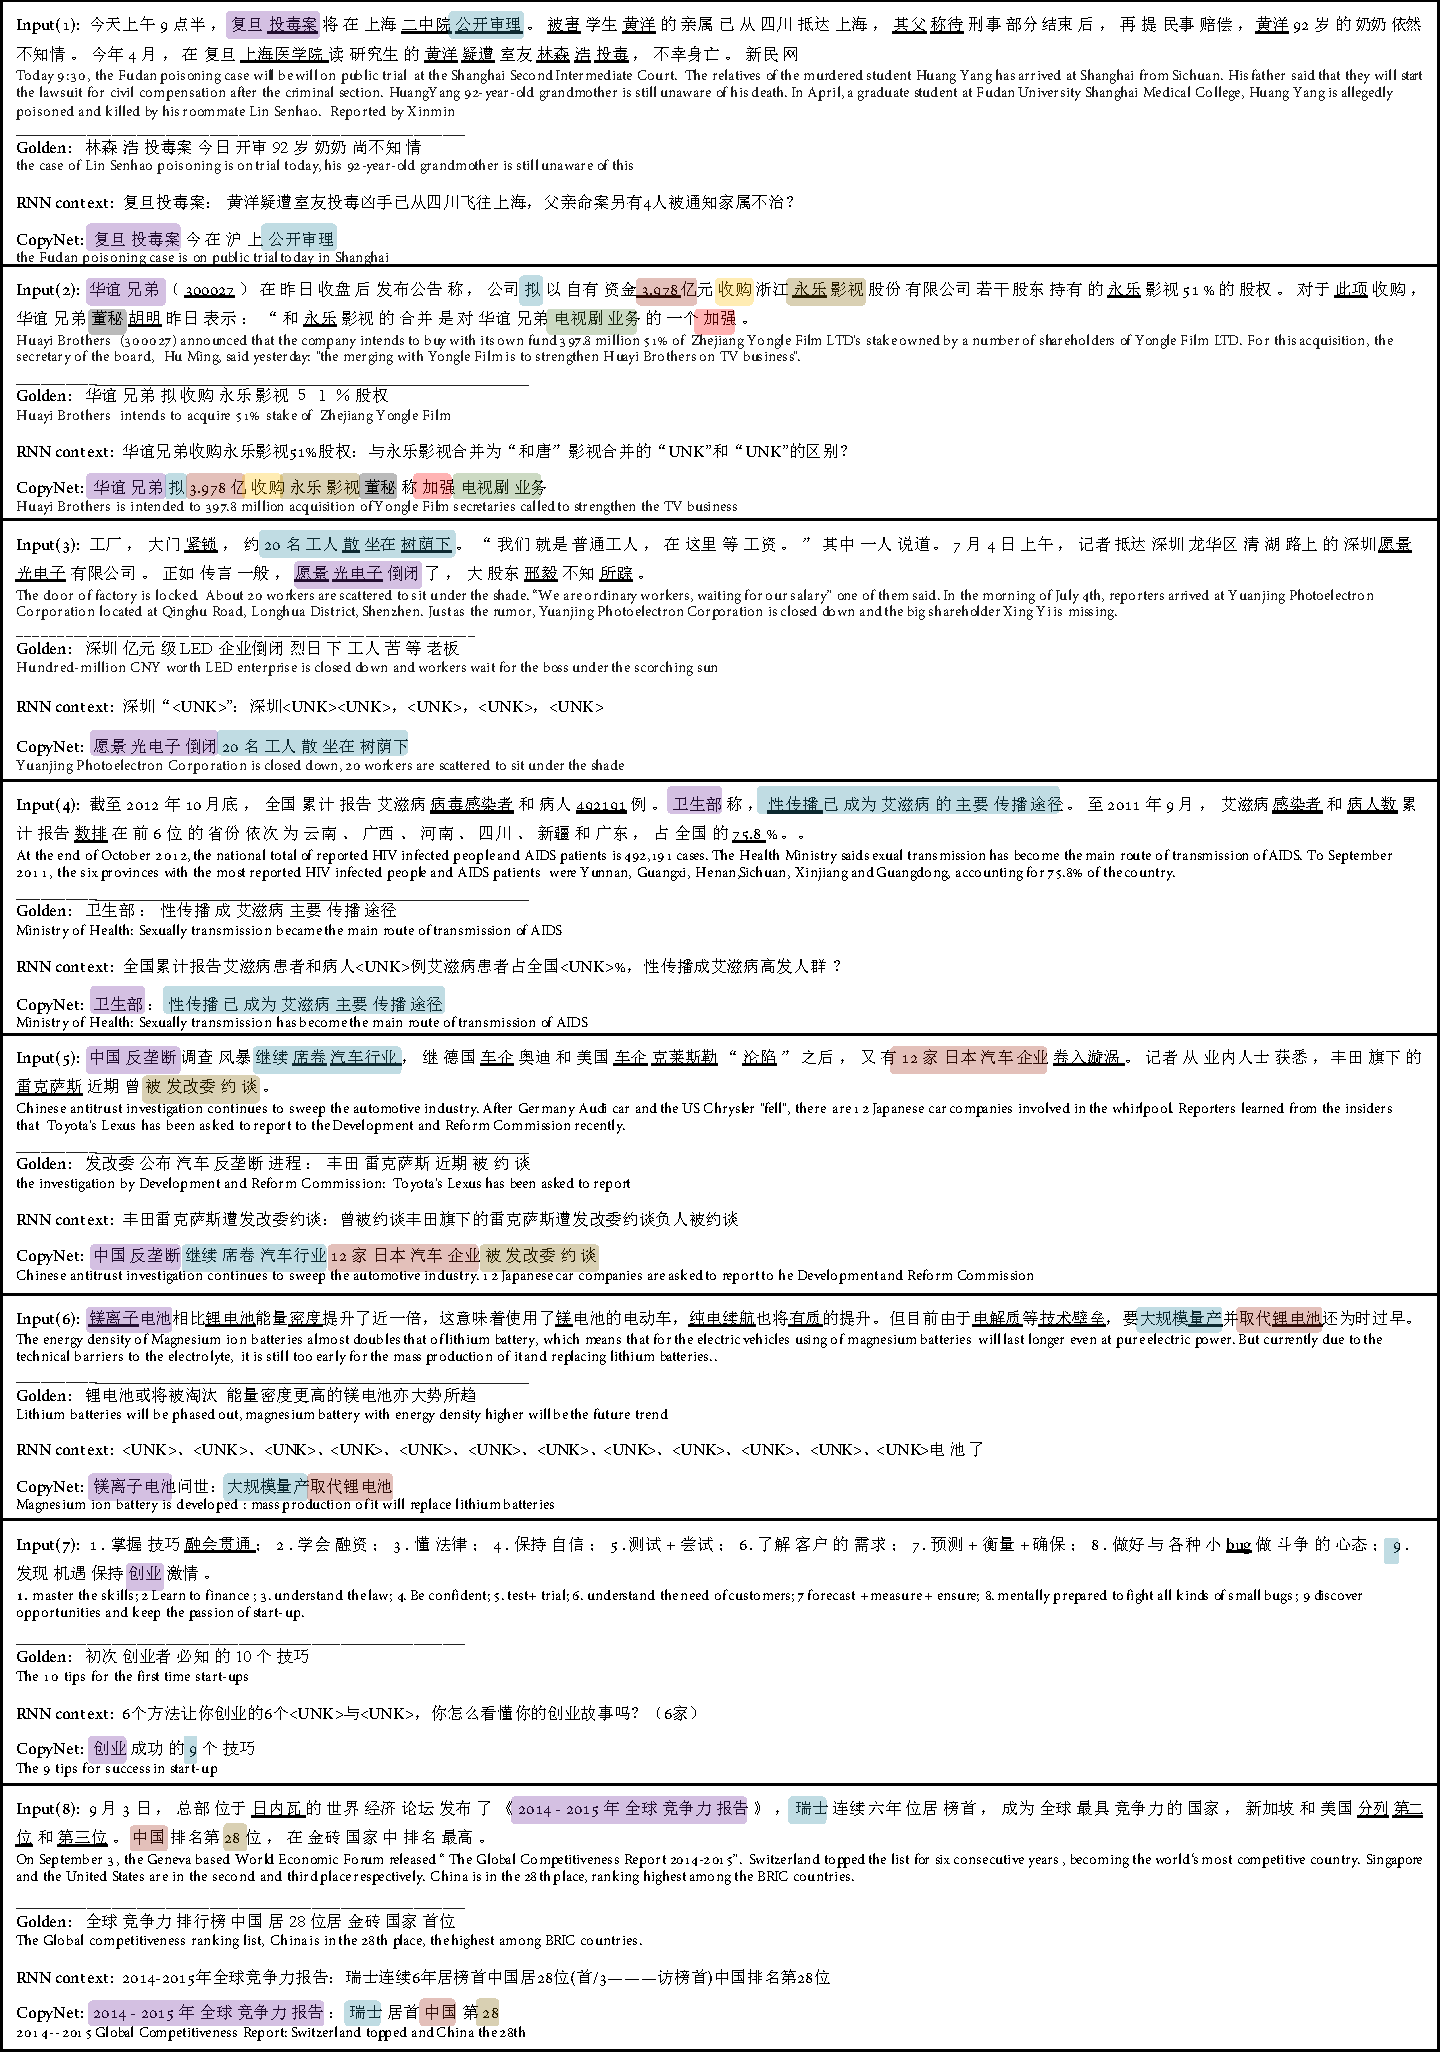
\includegraphics[width=0.85\linewidth]{figs/copynet/summaryXYZ.pdf}  
          	\caption{\label{cp3.fig.summary} Examples of \copynet on LCSTS compared with RNN context. Word segmentation is applied on the input, where underlined are OOV words. The highlighted words (with different colors) are those words with copy-mode probability higher than the generate-mode.  We also provide literal English translation for the document, the golden, and \copynet, while omitting that for RNN context since the language is broken.} 
  \end{figure}   

 \paragraph{Case Study}
As shown in Figure~\ref{cp3.fig.summary},  we make the following interesting observations about the summary from \copynet: 1) most words  are from copy-mode, but the summary is usually still fluent; 2) \copynet tends to cover consecutive words in the original document, but it often puts together segments far away from each other, indicating a sophisticated coordination of content-based addressing and location-based addressing; 3) \copynet handles OOV words really well: it can generate acceptable summary for document with many OOVs, and even the summary itself often contains many OOV words. In contrast, the canonical RNN-based approaches often fail in such cases.

It is quite intriguing that \copynet can often find important parts of the document, a behavior with the characteristics of extractive summarization, while it often  generate words to ``connect" those words, showing its aspect of abstractive summarization. %This makes it an elegant and powerful hybrid. 

%Due to the nature of task, \copynet often generate good summary but still vastly different the golden. Conversely, without a copying mechanism, RNNSearch works abnormally on complex input documents, especially when there exist many OOV words. Instead as shown in these examples, \copynet directly handles the OOV problem by copying without any bad affects.  
%The copied segments are separately distributed in the source document, and \copynet naturally learns to distinguish the important parts and extract them. We also find that  generate modes are sometimes activated to connect the extracted segments. Such behavior is quite similar with human when doing \textit{extractive} and \textit{abstractive} summarization together. 

\subsection{Single-turn Dialogue}
In this experiment we follow the work on neural dialogue model proposed in ~\cite{shang2015neural,vinyals2015neural,sordoni2015neural}, and test \copynet on single-turn dialogue. Basically, the neural model learns to generate a response to user's input, from the given (\textit{input}, \textit{response}) pairs as training instances.

\paragraph{Dataset}~ 
%Building a suitable real-world dataset for dialogue system is difficult since it contains too many noisy patterns, spoken language and external knowledge, which influences the demonstration of our model.  
 %As shown in Figure~\ref{ds}, 
 We build a simple dialogue dataset based on the following three instructions: 
%  \begin{figure}[htbp]
%   	\centering
%          	\vspace{-3pt}
%          	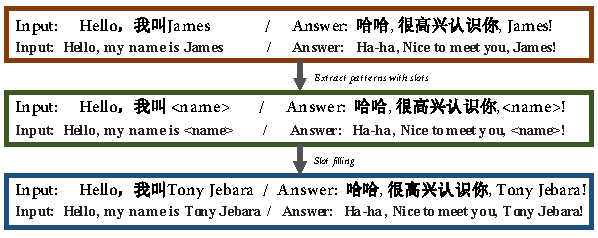
\includegraphics[width=.98\linewidth]{figs/copynet/ds.pdf} 
%          	\vspace{-5pt}
%          	\caption{\label{ds} Three steps to build the dialogue dataset} 
%   \vspace{-5pt}
%  \end{figure}   
  \begin{enumerate}
	\item Dialogue instances are collected from Baidu Tieba\footnote{http://tieba.baidu.com} with some coverage of conversations of real life, e.g., greeting and sports, etc.
	\item Patterns with slots like
	\[\texttt{hi, my name is } \mathbf{x}\rightarrow \texttt{hi, } \mathbf{x} 	 \]   
	are mined from the set, with possibly multiple responding patterns to one input.
	\item Similar with the synthetic dataset, we enlarge the dataset by filling the slots with suitable subsequence (e.g. name entities, dates, etc.)
\end{enumerate} 
%When filtering the retrieved answers, we focus on the answers that strongly related with the content of the posts, where a large proportion of answers contain the same substring with the input. Note that, 
To make the dataset close to the real conversations, we also maintain a certain proportion of instances with the response that 1) do not contain entities or 2) contain entities not in the input.  

\paragraph{Experimental Setting}~ We create two datasets: DS-\uppercase\expandafter{\romannumeral1} and DS-\uppercase\expandafter{\romannumeral2} with slot filling on 173 collected patterns. The main difference between the two datasets is that the filled substrings for training and testing in DS-\uppercase\expandafter{\romannumeral2} have no overlaps, while in DS-\uppercase\expandafter{\romannumeral1} they are sampled from the same pool. For each dataset we use 6,500 instances for training and 1,500 for testing. We compare \copynet with canonical RNNSearch, both character-based, with the same model configuration in \S\ref{cp3.sec.synthetic}. 

\begin{figure}[htbp]
   	\centering
          	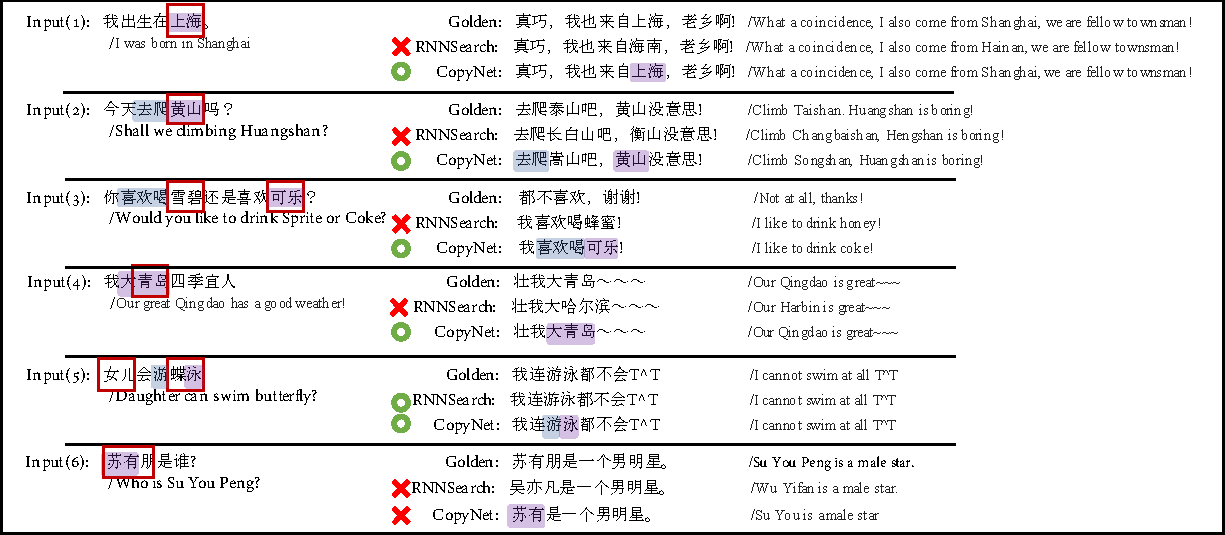
\includegraphics[width=.99\linewidth]{figs/copynet/ds-exp-rX.pdf} 
          	\caption{\label{cp3.fig.ds-exp} Examples on the testing set of DS-II shown as the input text and golden, with the outputs of RNNSearch and CopyNet. Words in red rectangles are unseen in the training set. The highlighted words (with different colors) are those words with copy-mode probability higher than the generate-mode. Green cirles (meaning correct) and red cross (meaning incorrect) are given based on human judgment on whether the response is appropriate. } 
  \end{figure}   


We compare \copynet and RNNSearch on DS-\uppercase\expandafter{\romannumeral1} and  DS-\uppercase\expandafter{\romannumeral2} in terms of top-1 and top-10 accuracy (shown in Table~\ref{cp3.table.ds-exp}), estimating respectively the chance of the top-1 or one of top-10 (from beam search) matching the golden. Since there are often many good responses to a input, top-10 accuracy appears to be closer to the real world setting. 

As shown in Table~\ref{cp3.table.ds-exp}, \copynet significantly  outperforms RNNsearch, especially on DS-\uppercase\expandafter{\romannumeral2}. It suggests that introducing the copying mechanism helps the dialogue system master the patterns in dialogue and correctly identify the correct parts of input, often proper nouns, to replicate in the response. Since the filled substrings have no overlaps in DS-\uppercase\expandafter{\romannumeral2}, the performance of RNNSearch drops significantly as it cannot handle words unseen in training data. In contrast, the performance of \copynet only drops slightly as it has learned to fill the slots with the copying mechanism and relies less on the representation of the words.

%%%%%%%%%%%%%%%%%%%%%%%%%%%%%%%%%%%%%%%%%%%%%%%%
\begin{table}[htpb] % "[h!]" location specifier just for this example
\centering
\begin{tabular}{lccccc}
\toprule
 &\multicolumn{2}{c}{DS-\uppercase\expandafter{\romannumeral1}~(\%)}
 && \multicolumn{2}{c}{DS-\uppercase\expandafter{\romannumeral2}~(\%)}\\
%\cmidrule{2-3}
\cmidrule{2-3}\cmidrule{5-6}
Models &Top1&Top10 &&Top1 &Top10	\\
\midrule
RNNSearch &  44.1 & 57.7 && 13.5 & 15.9 \\
\copynet & \textbf{61.2} & \textbf{71.0}  && \textbf{50.5} & \textbf{64.8} \\										  
\bottomrule
\end{tabular} 
\caption{\label{cp3.table.ds-exp} The decoding accuracy on the two testing sets. Decoding is admitted success only when the answer is found exactly in the Top-K outputs. }
\end{table} 
 %%%%%%%%%%%%%%%%%%%%%%%%%%%%%%%%%%%%%%%%%%%%%%%%
%\\\vspace{-7pt} \\
\paragraph{Case Study}~ As indicated by the examples in  Figure~\ref{cp3.fig.ds-exp}, \copynet accurately replicates the critical segments from the input with the copy-mode, and generates the rest of answers smoothly through the generate-mode. Note that in (2) and (3), the decoding sequence is not exactly the same with the standard one, yet still correct regarding to their meanings. In contrast, although RNNSearch usually generates answers in the right formats, it fails to catch the critical entities in all three cases because of the difficulty brought by the unseen words.

%\begin{equation}
%	\nabla_{\theta} L= \sum_{k=1}^{K}\nabla_{\theta} {\log(a_k)}(R - b) 
%\end{equation}


\section{Related Work}
Our work is partially inspired by the recent work of Pointer Networks~\cite{vinyals2015pointer}, in which a pointer mechanism (quite similar with the proposed copying mechanism) is used to predict the output sequence directly from the input. In addition to the difference with ours in application, \newcite{vinyals2015pointer} cannot predict outside of the set of input sequence, while \copynet can naturally combine generating and copying.  

\copynet is also related to the effort to solve the OOV problem in neural machine translation. \newcite{luong-EtAl:2015:ACL-IJCNLP} introduced a heuristics to post-process the translated sentence using annotations on the source sentence. In contrast \copynet addresses the OOV problem in a more systemic way with an end-to-end model. However, as \copynet copies the exact source words as the output, it cannot be directly applied to machine translation. However, such copying mechanism can be naturally extended to any types of references except for the input sequence, which will help in applications with heterogeneous source and target sequences such as machine translation.

The copying mechanism can also be viewed as carrying information over to the next stage without any nonlinear transformation.  Similar ideas are proposed for training very deep neural networks in \cite{srivastava2015highway,he2015deep} for classification tasks, where shortcuts are built between layers for the direct carrying of information.  Copying from the source sequence can also be seen as a special effort to utilise ``memory'', as we discussed as a hybrid representation of short-term memory in \sts learning framework, sharing some similarity with memory-based approaches like \cite{weston2014memory,sukhbaatar2015end,graves2014neural}



%Our work is also inspired by the explicit design on combining content-based addressing together with location-based addressing, which is explored in~\cite{graves2014neural,kurach2015neural}. In addition,  combining ``hard operation" like the copying mechanism in neural networks is also researched for question answering with knowledge bases in~\cite{neelakantan2015neural,yin2015neural2,yin2015neural}
\section{Conclusion and Next Chapter}
In this chapter, we proposed \copynet to incorporate copying into the sequence-to-sequence learning framework.  \copynet can nicely integrate the regular way of word generation in the decoder with the new copying mechanism which can choose sub-sequences in the input sequence and put them at proper places in the output sequence. Our empirical study on both synthetic data sets and real world data sets demonstrates the efficacy of \copynet. 

However, we did not discuss about the application of \copynet in neural machine translation which is the main focus of this thesis. Because the copying mechanism requires the source and the target sequences at least share the same sub-sequences, which is not the case for  task where the source and target are in  heterogeneous types, for example, machine translation. One of the options is to use a dictionary to replace the source words with its word-level translation so that we can apply the same copying mechanism in NMT~\cite{gulcehre2016pointing}, which, however, is limited to the accuracy of word-level dictionary. 

In the next chapter, we extend the ``copying mechanism'' in a principle way for neural machine translation where we incorporate a search-engine by searching similar translation pairs to guide the NMT system so that it can achieve a better efficiency of using the data.

\chapter[Non-Parametric Neural Machine Translation]{Search-Engine Guided Non-Parametric Neural Machine Translation}
\label{seg-nmt}
\section{Overview}

As discussed in previous chapters, as a typical type of \sts learning,
%neural machine translation is a recently proposed paradigm in machine translation, where a single neural network, often consisting of encoder and decoder recurrent networks, is trained end-to-end to map from a source sentence to its corresponding translation\citep{bahdanau2014neural,cho2014learning,sutskever2014sequence,kalchbrenner2013recurrent}. 
the success of neural machine translation~\citep{bahdanau2014neural}, which has already been adopted by major industry players in machine translation\citep{wu2016google,crego2016systran,hassan-hp}, is often attributed to the advances in building and training recurrent networks as well as the availability of large-scale parallel corpora for machine translation. However, it usually fails to work well for translation in special domains (e.g. law),  as it lacks enough data to learn many professional expressions.

Neural machine translation is most characteristically distinguished from the existing approaches to machine translation, such as phrase-based statistical machine translation\citep{koehn2003statistical}, in that it projects a sequence of discrete source symbols into a continuous space and decodes back the corresponding translation. This allows one to easily incorporate other auxiliary information into the neural machine translation system as long as such auxiliary information could be encoded into a continuous space using a neural network. This property has been noticed recently and used for building more advanced translation systems such as multilingual translation~\citep{firat2016multi,luong2015multi}, multi-source translation~\citep{zoph2016multi,firat2016zero}, multimodal translation~\citep{caglayan2016does} and syntax guided translation~\citep{nadejde2017syntax,eriguchi2017learning}. 

In this chapter, we first notice that this ability in incorporating arbitrary meta-data by neural machine translation allows us to naturally extend it to a non-parametric
model in which a neural machine translation system explicitly takes into account a full training set consisting of source-target sentence pairs (in this paper we refer them as a general translation memory). We can build a neural machine translation system that considers not only a given source sentence, which is to be translated but also a set of training sentence pairs in the process of translation. To do so, we propose a novel extension of attention-based neural machine translation that seamlessly fuses two information streams, each of which corresponds to the current source sentence and a set of training sentence pairs, respectively. The \textit{copying mechanism} that is introduced in Chapter~\ref{copy} is adopted for fusing the information of the two streams.  
\begin{figure}[t]
	\centering
	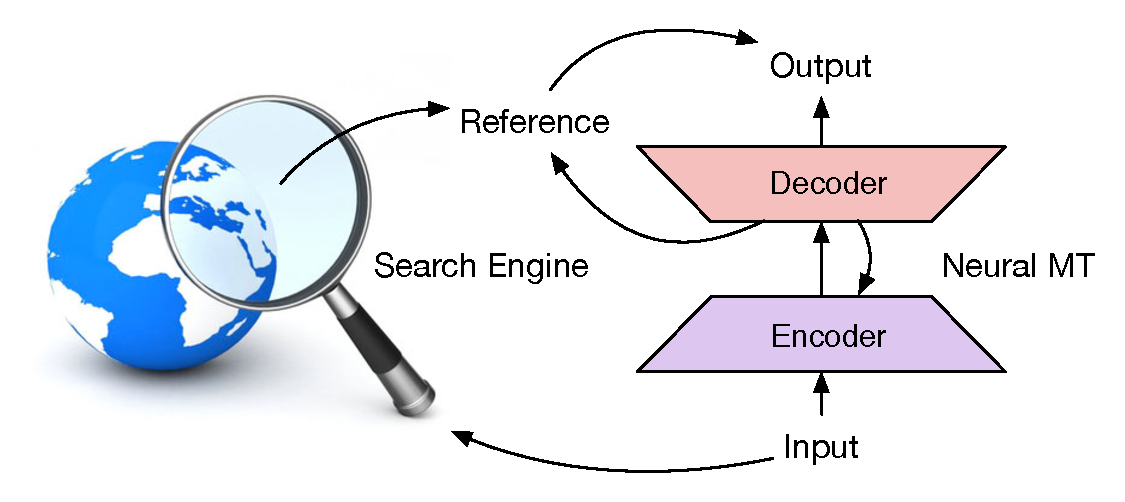
\includegraphics[width=0.8\textwidth]{figs/seg/picture}
	\caption{\label{cp4.fig.illustration}An illustration of the proposed search-engine guided non-parametric neural machine  translation.}
\end{figure}

A major technical challenge, other than designing such a neural machine translation system, is the scale of a training parallel corpus which often consists of hundreds of thousands to millions of sentence pairs. We address this issue by incorporating an off-the-shelf black-box search engine into the proposed neural machine translation system. The proposed approach first queries a search engine, which indexes a whole training set, with a given source sentence, and the proposed neural translation system translates the source sentence while incorporating all the retrieved training sentence pairs. In this way, the proposed translation system automatically adapts to the search engine and its ability to retrieve relevant sentence pairs from a training corpus. See Fig.~\ref{cp4.fig.illustration} as an illustration of the proposed system.

We evaluate the proposed search-engine guided non-parametric neural machine translation (SEG-NMT) on three language pairs (En-Fr, En-De, and En-Es, in both directions) from JRC-Acquis Corpus\citep{steinberger2006jrc} which consists of documents from a legal domain. This corpus was selected to demonstrate the efficacy of the proposed approach when a training corpus and a set of test sentences are both from a similar domain. Our experiments reveal that the proposed approach exploits the availability of the retrieved training sentence pairs very well, achieving significant improvement over the strong baseline of attention-based neural machine translation\citep{bahdanau2014neural}.

\subsection{Background: Translation Memory}
Our proposed research of the search-engine guided translation is also strongly corresponded to the usage of the ``translation memory'' in machine translation.
Translation memory is a computer-aided translation tool widely used by professional human translators. It is a database of pairs of source phrase and its translation. This database is constructed incrementally as a human translator translates sentences. When a new source sentence is present, a set of (overlapping) phrases from the original sentence are queried against the translation memory, and the corresponding entries are displayed to the human translator to speed up the process of translation. Due to the problem of sparsity, exact matches rarely occur, and approximate string matching is often used.

In this chapter, we consider a more general notion of translation memory in which not only translation phrase pairs but any kind of translation pairs are stored. In this more general definition, a training parallel corpus is also considered a translation memory. This saves us from building a phrase table\citep{koehn2003statistical}, which is yet another active research topic, but requires us to be efficient and flexible in retrieving relevant translation pairs given a source sentence, as the issue of data sparsity amplifies. This motivates us to come up with an efficient query algorithm tied together with a downstream translation model that can overcome the problem of data sparsity.

\begin{figure}[hptb]
%\label{framework}
%\begin{minipage}{0.82\textwidth}
% \vspace{-10pt}
\centering
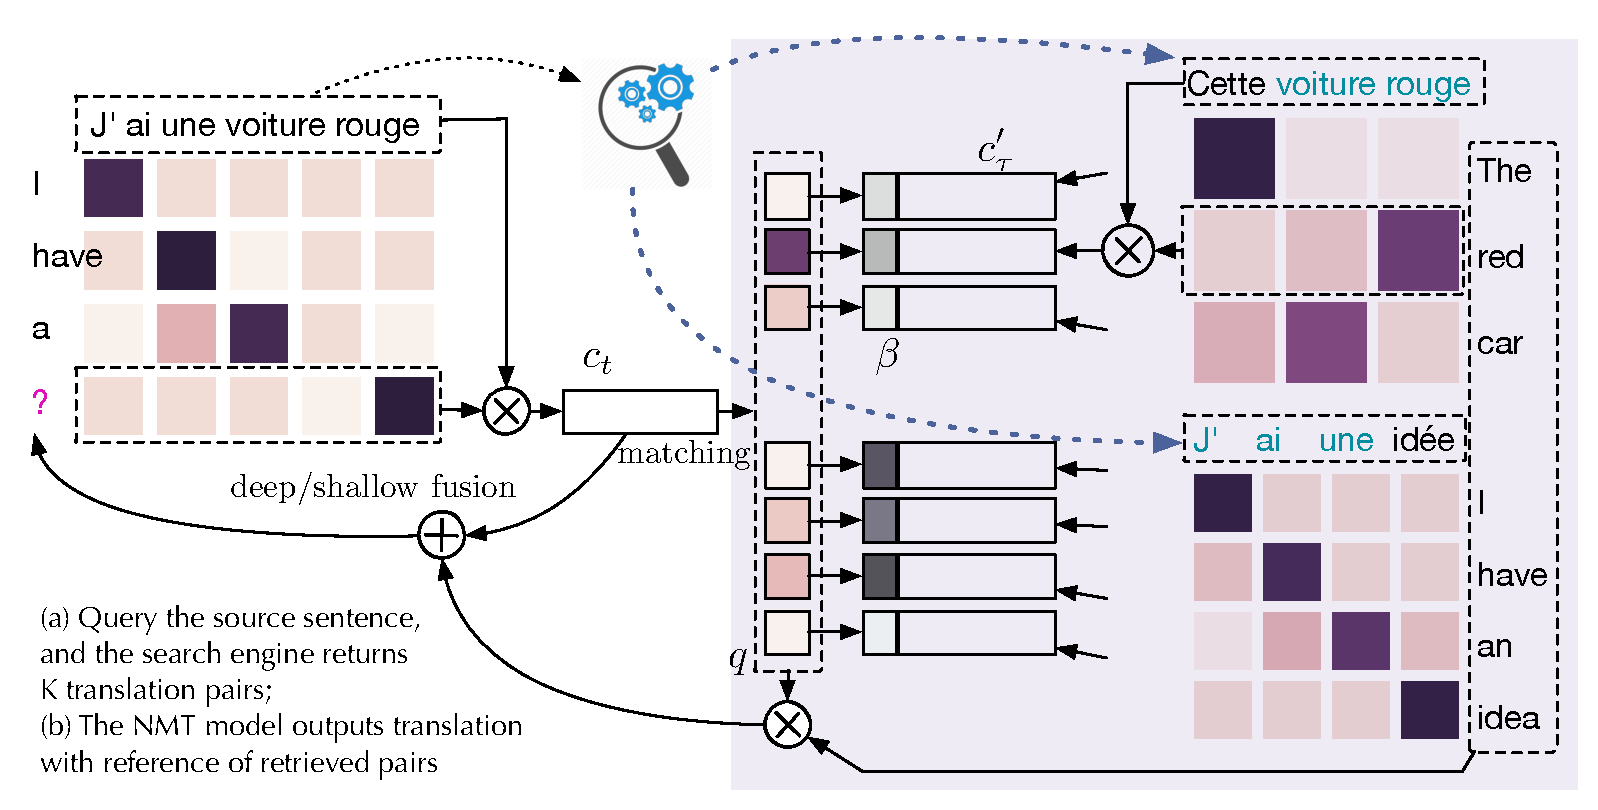
\includegraphics[width=\linewidth]{figs/seg/framework2.pdf}
%\end{minipage}
%\hfill
%\begin{minipage}{0.17\textwidth} 
\caption{\label{cp4.fig.tmnmt} The overall architecture of the proposed SEG-NMT. The shaded box includes the module which handles a set of translation pairs retrieved in the first stage. The heat maps represent the attention scores between the source sentences (left-to-right) and the corresponding translations (top-to-down).}
%\end{minipage}
% \vspace{-4mm}
\end{figure}


\section{Search Engine Guided Non-Parametric Neural Machine Translation}

%\vspace{-3pt}
We propose a non-parametric
neural machine translation model guided by an off-the-shelf, efficient search engine. Unlike the conventional neural machine translation system, the proposed model does not discard a training corpus but maintain and actively exploit it in the test time. This effectively makes the proposed neural translation model a fully non-parametric model.

The proposed nonparametric
neural translation model consists of two stages. The first stage is a retrieval stage, in which the proposed model queries a training corpus, or equivalently a translation memory, to retrieve a set of source-translation pairs given a current source sentence. To maximize the computational efficiency, first we utilize an off-the-shelf, highly-optimized search engine to quickly retrieve a large set of similar source sentences, and their translations, after which the top-$K$ pairs are selected using approximate string matching based on edit distance. 

In the second stage, a given source sentence is translated by an attention-based neural machine translation model, which we refer to as a {\it search engine guided neural machine translation} (SEG-NMT), and incorporates the retrieved translation pairs from the first stage. In order to maximize the use of the retrieved pairs, we build a novel extension of the attention-based model that performs attention not only over the source symbols but also over the retrieved symbols (and their respective translations). We further allow the model to \textit{copy} over a target symbol directly from the retrieved translation pairs. The overall architecture with a simple translation example of the proposed SEG-NMT is shown in Fig.~\ref{cp4.fig.tmnmt} for reference.


% \begin{wrapfigure}{R}{0.5\textwidth}
% \vspace{-4mm}
% \begin{minipage}{0.5\textwidth}
% \end{minipage}
% \vspace{-3mm}
% \end{wrapfigure}


%\vspace{-3pt}
\subsection{Retrieval Stage}

We refer to the first stage as a {\it retrieval stage}. In this stage, we go over the entire training set $\mathcal{M}=\left\{ (X^n, Y^n)\right\}_{n=1}^N$ to find pairs whose source side is similar to a current source $X$. That is, we define a similarity function $\calS(X, X')$, and find $(X^n, Y^n)$ where $\calS(X, X^n)$ is large. 

%\vspace{-7pt}
\paragraph{Similarity score function $\calS$}

In this paper, we constrain ourselves to a setting in which only a neural translation model is trainable. That is, we do not assume the availability of other trainable sentence similarity functions. This allows us to focus entirely on the effectiveness of the proposed algorithm while being agnostic to the choice of similarity metric. Under this constraint, we follow an earlier work by \citep{li2016phrase} and use a fuzzy matching score which is defined as 
\begin{align}
\label{cp4.eq.fuzzy}
\calS_{\text{fuzzy}}(X, X') = 1 - \frac{\calD_{\text{edit}}(X, X')}{\max\left(|X|, |X'|\right)},
\end{align}
where $\calD_{\text{edit}}$ is an edit distance and $| \cdot |$ shows the sentence length. 

\begin{algorithm}[htpb]
\caption{Greedy selection procedure to maximize the coverage of the source symbols.} %\alert{KC: put details of each symbol inside the algorithm.}}
\label{cp4.algo.alg1}
\begin{algorithmic}[1]
\small
\Require{input $X$, translation memory $\mathcal{M}$}
\State Obtain the subset $\tilde{M}\subseteq M$ using an off-the-shelf search engine;
\State Re-rank retrieved pairs $\left(X', Y' \right) \in \tilde{M}$ using the similarity score function $\calS$ in descending order;
\State Initialize the dictionary of selected pairs $R = \emptyset$; 
\State Initialize the coverage score $c=0$;
\For{$k=1...|\tilde{M}|$}  
\State $c_{\text{tmp}}= \sum_{x \in X}\delta\left[ x \in R.\text{keys} \cup \{X'_k\}\right]/|X|$
\If{$c_{\text{tmp}}> c$} 
\State $c = c_{\text{tmp}}$; $R \leftarrow \{X'_k: Y'_k\}$
\EndIf
\EndFor
\State \textbf{return} $R$
\end{algorithmic}
\end{algorithm}


\paragraph{Off-the-shelf Search Engine}

The computational complexity of the similarity search grows linearly with the size of the translation memory which in our case contains all the pairs from a training corpus. Despite the simplicity and computational efficiency of the similarity score in Eq.~\eqref{cp4.eq.fuzzy}, this is clearly not practical, as the size of the training corpus is often in the order of hundreds of thousands or even tens of millions. We overcome this issue of scalability by incorporating an off-the-shelf search engine, more specifically Apache Lucene.\footnote{
\url{https://lucene.apache.org/core/}
} 
We then use Lucene to retrieve an initial set of translation pairs based on the source side, and use the similarity score above to re-rank them. 


\paragraph{Final selection process}
Let $\tilde{\mathcal{M}} \in \mathcal{M}$ be an initial set of translation pairs returned by Lucene. We rank the translation pairs within this set by $\calS(X, X')$. We design and test two methods for selecting the final set from this initial set based on the similarity scores. The first method is a top-$K$ retrieval, where we simply return the $K$ most similar translation pairs from $\tilde{\mathcal{M}}$. The second method returns an adaptive number of translation pairs based on the coverage of the symbols $x$ in the current source sentence $X$ within the retrieved translation pairs. We select greedily starting from the most similar translation pair, as described in Alg.~\ref{cp4.algo.alg1}. 


\subsection{Translation Stage} 
In the second stage, we build a novel extension of the attention-based neural machine translation, SEG-NMT, that seamlessly fuses both a current source sentence and a set $\hat{M}$ of retrieved translation pairs. In a high level, the proposed SEG-NMT first stores each target symbol of each retrieved translation pair into a key-value memory~\citep{miller2016key}. At each time step of the decoder, SEG-NMT first performs attention over the current source sentence to compute the time-dependent context vector based on which the key-value memory is queried. SEG-NMT fuses information from both context vector of the current source sentence and the retrieved value from the key-value memory to generate a next symbol. 

\paragraph{Key-Value Memory}

For each retrieved translation pair $(X', Y') \in \hat{\mathcal{M}}$, we run a full attention-based neural machine translation model,\footnote{
We use a single copy of attention-based model for both key extraction and translation.
}
specified by a parameter set $\theta$, and obtain, for each target symbol $y'_t \in Y'$, a decoder's hidden state $z'_t$ and an associated time-dependent context vector $c'_t$ (see Eq.~\eqref{cp2.eq.att} in Chapter~\ref{background} which summarizes a subset of the source sentence $X'$ that best describes $y'_t$). We consider $c'_t$ as a key and $(z'_t, y'_t)$ as a value, and store all of them from all the retrieved translation pairs in a key-value memory. Note that this approach is agnostic to how many translation pairs were retrieved during the first stage.


\paragraph{Matching and Retrieval}

At each time step of the SEG-NMT decoder, we first compute the context vector $c_t$ as in Eq.~\eqref{cp2.eq.att}. This context vector is used as a key for querying the key-value memory. Instead of hard matching, we propose {\it soft matching} based on a bilinear function, where we compute the matching score of each key-value slot by
\begin{equation}
\label{cp4.eq.score}
    %q_{t, \tau}  = \frac{\exp\{E(c_t, c'_\tau)\}}{\sum_{\tau'} \exp\{E(c_t, c'_{\tau'})\}}.
	q_{t, \tau}  = \ssoftmax_{\tau}\left(c_t^{\top}\cdot A \cdot c'_\tau\right)
\end{equation}
%where $E(c_t, c'_\tau) = c_t^{\top}A c'_\tau$ and 
where $A$ is a trainable matrix. 
These scores are used to retrieve a value from the key-value memory. In the case of the decoder's hidden states, we retrieve a weighted sum:
\begin{equation}
	\tilde{z}_t = \sum_{\tau} q_{t, \tau} \cdot z'_{\tau}.
\end{equation}
In the case of target symbols, we consider each  score as a probability of the corresponding target symbol. That is,
$p_{\text{copy}}(y_{\tau}'|\mathcal{M}) = q_{t, \tau},$ as the {\it copying mechanism} proposed in the previous chapter.

% \begin{wrapfigure}{R}{0.54\textwidth}
% \vspace{-22pt}
% \begin{minipage}{0.54\textwidth}
% \end{minipage}
% \vspace{-5pt}
% \end{wrapfigure}


\paragraph{Incorporation}

We consider two separate approaches to incorporating the retrieved values from the key-value memory. The first approach, called {\it deep fusion}, weighted-average the retrieved hidden state $\tilde{h}_t$ and the decoder's hidden state $h_t$:
\begin{align}
\label{cp4.eq.deep}
z_{\text{fusion}} = &\zeta_t \cdot \tilde{z}_t + (1 -\zeta_t) \cdot z_t 
\end{align}
when computing the output distribution $p(y_t|y_{0:t-1}, x_{1:T'},\mathcal{M})$ (see Eq.~\eqref{cp2.eq.output}). 

The second approach, which is the main method we used, is called {\it shallow fusion} and computes the output distribution as a mixture of probability:
\begin{align}
\label{cp4.eq.shallow}
p(y_t| y_{0:t-1}, x_{1:T'}, \mathcal{M}) = \zeta_t \cdot p_{\text{copy}}(y_t|\mathcal{M}) + (1-\zeta_t) \cdot p(y_t|y_{0:t-1}, x_{1:T'}).
\end{align}
This is equivalent to have a option for copying over a retrieved the target symbol $y_{\tau}'$ with the probability of $ p_{\text{copy}}(y_{\tau})$ as the next target symbol~\citep{gu2016incorporating}. In this case, the proposed SEG-NMT is a direct extension of \copynet  in the scenario of NMT. % We can build a SEG-NMT by using either or both of these approaches.

In both of the approaches, there is a gating variable $\zeta_t$. As each target symbol may require a different source of information, we let this variable be determined automatically by the proposed SEG-NMT. That is, we introduce another feedforward network that computes $\zeta_t = f_{\text{gate}}(c_t, z_t, \tilde{z}_t)$. This gate closes when the retrieved pairs are not useful for predicting the next target symbol $y_t$, and opens otherwise. 

\begin{algorithm}[hpbt]
\caption{Learning for SEG-NMT}% \alert{TODO: if there's not enough space, we should move this to a supplementary material.}}
\label{cp4.algo.alg2}
\begin{algorithmic}[1]
\small
\Require{Search engine  $F_{SS}$, MT model ${\theta}$, SEG model ${\theta'}$, $A, \lambda, \eta$, parallel training set $D$,  translation memory $\mathcal{M}$.}
\State Initialize $\phi = \{\theta, \theta', A, \lambda, \eta\}$;
\State Set the number of returned answers as $K$;
\While{stopping criterion is not met}
\State Draw a translation pair: $(X, Y)\sim D$;
\State Obtain memory pairs $\{X'_k, Y'_k\}_{k=1}^K = F_{SS}(X, \mathcal{M})$
\State Reference Memory $C=\emptyset$.
\For{$k=1...K$}   \quad \quad \# generate dynamic keys
\State Let $Y'_k = \{y'_1, ..., y'_{T_k}\}, X'_k = \{x'_1, ..., x'_{T'_k}\}$
\For{$\tau=1...T_k$}
\State Generate key $c'_\tau = f^{\textsc{att}}(y'_{0:\tau-1}, x'_{1:T'_k})$\footnote{For simplicity, we use a slightly different formulation of $f^{\textsc{att}}$ in Eq.~\eqref{cp2.eq.att}.}
\State Initialize coverage $\beta_{\tau} = 0.$
\State $ C \leftarrow (c'_\tau, y'_\tau, \beta_{\tau})$
\EndFor 
\EndFor
\State Let $Y = \{y_1, ..., y_{T}\}, X = \{x_1, ..., x_{T'}\}$
\For{$t=1...T$} \quad \quad \# translate each word
\State Generate query $c_t = f^{\textsc{att}}(y_{0:t-1}, x_{1:T'})$
\For{$\tau=1... | C | $}  Read $c'_\tau, y'_\tau,  \beta_{\tau} \in C$
\State Compute the score $q_{t, \tau}$ using Eq.~\ref{cp4.eq.match};
\State Gompute the gate $\zeta_t$ with $f_{\text{gate}}$;
\State Update $\beta_{\tau} \leftarrow \beta_{\tau} + q_{t, \tau}\cdot\zeta_t$;
\EndFor
\State Compute the probability $p(y_t|\cdot)$
\State \hspace{10pt} --option1: shallow-fusion, Eq.~\ref{cp4.eq.shallow}
\State  \hspace{10pt} --option2: deep-fusion, Eq.~\ref{cp4.eq.deep}
\EndFor 
\State Update $\phi \leftarrow \phi  +\gamma\frac{\partial}{\partial \phi} \sum_{t=1}^T\log p(y_t|\cdot)$
\EndWhile
\end{algorithmic}
\end{algorithm}

\paragraph{Coverage}

In the preliminary experiments, we notice that the access pattern of the key-value memory was highly skewed toward only a small number of slots. Motivated by the coverage penalty from \citep{tu2016modeling}, we propose to augment the bilinear matching function (in Eq.~\eqref{cp4.eq.score}) with a coverage vector $\beta_{t,\tau}$ such that

\begin{align}
\label{cp4.eq.match}
     q_{t, \tau}  = \ssoftmax_{\tau'}\left(c_t^\top \cdot M \cdot c'_\tau - \lambda \beta_{t-1, \tau}\right),
\end{align}
where  $\lambda$ is a trainable parameter, and the coverage vector is defined as 
\begin{equation}
	 \beta_{t, \tau}= \sum_{t'=1}^t q_{t', \tau}\cdot\zeta_{t'}.
\end{equation}

\section{Learning and Inference}
The proposed model, including both the first and second stages, can be trained end-to-end to maximize the log-likelihood given a parallel corpus. For practical training, we preprocess a training parallel corpus by augmenting each sentence pair with a set of translation pairs retrieved by a search engine, while ensuring that the exact copy is not included in the retrieved set. See Alg.~\ref{cp4.algo.alg2} for a detailed description. 

During inference, we search through the whole training set to retrieve relevant translation pairs. Similarly to a standard neural translation model, we use beam search (as noted in \S\ref{cp2.sec.bs})  to decode the best translation given a source sentence. 


%\vspace{-3pt}
\section{Experiments}
%\vspace{-3pt}
\subsection{Settings}
\paragraph{Data}

We use the JRC-Acquis corpus\citep{steinberger2006jrc} for evaluating the proposed SEG-NMT model.\footnote{
\url{http://optima.jrc.it/Acquis/JRC-Acquis.3.0/corpus/}
} The JRC-Acquis corpus consists of the total body of European Union (EU) law applicable to the member states. The text in this corpus is well structured, and most of the text in this corpus are related, making it an ideal test bed to evaluate the proposed SEG-NMT which relies on the availability of appropriate translation pairs from a training set. 
This corpus also contained  many professional expressions which is difficult for neural models to remember, but easy to {\it copy} similar translation pairs.
This corpus was also used by \citep{li2016phrase} in investigating the combination of translation memory and phrase-based statistical machine translation, making it suitable for our proposed method to evaluate on. 

\begin{table}[htpb]
\centering
\begin{tabular}{l|r|r|r}
\toprule
 Dataset& En-Fr & En-De  & En-Es\\
\midrule
\# Train Pairs &744,528 &717,096 &697,187 \\
\# Dev Pairs &2,665 &2,454 &2,533  \\
\# Test Pairs &2,655 &2,483 &2,596  \\
\midrule
\# En/sent. &29.44&33.43 &32.10  \\
\# Other/sent. &33.34 &33.44 &34.95  \\
\bottomrule
\end{tabular}
\caption{\label{cp4.table.dataset} Statistics from the JRC-Acquis corpus. We use BPE subword symbols.}
\end{table}

We select three language pairs, namely, En-Fr, En-Es, and En-De, for evaluation. For each language pair, we uniformly select 3000 sentence pairs at random for both the development and test sets. The rest is used as a training set, after removing any sentence which contains special characters only. We use sentences of lengths up to 80 and 100 from the training and dev/test sets respectively. We do not lowercase the text, and use byte-pair encoding (BPE)\citep{sennrich2015neural} to extract a vocabulary of 20,000 subword symbols. See Table~\ref{cp4.table.dataset} for detailed statistics.

%\vspace{-9pt}
\paragraph{Retrieval Stage}

We use Apache Lucene to index a whole training set and retrieve 100 pairs per source sentence for the initial retrieval. These 100 pairs are scored against the current source sentence using the fuzzy matching score from Eq.~\eqref{cp4.eq.fuzzy} to select top-$K$ relevant translation pairs. We vary $K$ among $1$ and $2$ during training and among $1, 2, 4, 8, 16$ during testing to investigate the trade-off between retrieval and translation quality. During testing, we also evaluate the effect of adaptively deciding the number of retrieved pairs using the proposed greedy selection algorithm (Alg.~\ref{cp4.algo.alg1}). 

%\vspace{-9pt}
\paragraph{Translation Stage}

We use a standard attention-based NMT model~\citep{bahdanau2014neural} with 1,024 gated recurrent units(GRU)\citep{cho2014learning} on each of the encoder and decoder. We train both the vanilla model as well as the proposed SEG-NMT based on this configuration from scratch using Adam~\citep{kingma2014adam} with the initial learning rate set to 0.001. We use a minibatch of up to 32 sentence pairs. We early-stop based on the development set performance. We use beam search with width 5 for evaluation.

In the case of the proposed SEG-NMT, we parametrize the metric matrix $M$ in the similarity score function from Eq.~\eqref{cp4.eq.match} to be diagonal and initialized to an identity matrix. $\lambda$ in Eq.~\eqref{cp4.eq.match} is initialized to $0$. The gating network $f_{\text{gate}}$ is a feedforward network with a single hidden layer, just like the attention mechanism $f_{\text{att}}$. We use either deep fusion or shallow fusion in our experiments.

\subsection{Result and Analysis}
%\vspace{-3pt}
% \begin{wraptable}{R}{0.61\textwidth} 
\begin{table}
%\vspace{-4mm}
  \centering
    \begin{tabular}{l|l|cc|cc|cc}
    \toprule
    \multicolumn{2}{c|}{\multirow{2}[2]{*}{}} & \multicolumn{2}{c|}{En-Fr} & \multicolumn{2}{c|}{En-De} & \multicolumn{2}{c}{En-Es} \\
    \multicolumn{2}{c|}{} & \multicolumn{1}{c}{$\rightarrow$} & \multicolumn{1}{c|}{$\leftarrow$}  & \multicolumn{1}{c}{$\rightarrow$} & \multicolumn{1}{c|}{$\leftarrow$} & \multicolumn{1}{c}{$\rightarrow$} & \multicolumn{1}{c}{$\leftarrow$} \\
    \midrule
    \multirow{3}[2]{*}{\rotatebox{90}{Dev}} 
         & TM    & \multicolumn{1}{c}{46.62} & 42.53 & \multicolumn{1}{c}{34.99} & \multicolumn{1}{c|}{42.45} & \multicolumn{1}{c}{40.84} & \multicolumn{1}{c}{39.71} \\
         & NMT   & \multicolumn{1}{c}{58.95} & 59.69 & \multicolumn{1}{c}{44.94} & \multicolumn{1}{c|}{50.20} & \multicolumn{1}{c}{50.54} & \multicolumn{1}{c}{55.02} \\
         & \copynet & \multicolumn{1}{c}{60.34} & 61.61 & - & - & - & -\\
         & SEG-NMT & \multicolumn{1}{c}{\textbf{64.16}} & \textbf{64.64} & \multicolumn{1}{c}{\textbf{49.26}} & \multicolumn{1}{c|}{\textbf{55.63}} & \multicolumn{1}{c}{\textbf{57.62}} & \multicolumn{1}{c}{\textbf{60.28}} \\
    \midrule
    \multirow{3}[2]{*}{\rotatebox{90}{Test}}
             & TM    & \multicolumn{1}{c}{46.64} & 43.17 & \multicolumn{1}{c}{34.61} & \multicolumn{1}{c|}{41.83} & \multicolumn{1}{c}{39.55} & \multicolumn{1}{c}{37.73} \\
          & NMT   &   59.42    &  60.11     &   43.98    &   49.74   &   50.48    &  54.66\\
          & \copynet & \multicolumn{1}{c}{60.55} & 62.02 & - & - & - & -\\
          & SEG-NMT & \textbf{64.60} & \textbf{65.11} & \textbf{48.80}  &  \textbf{55.33}  &  \textbf{57.27}  &  \textbf{59.34} \\
    \bottomrule
    \end{tabular}%
     \caption{The BLEU scores on JRC-Acquis corpus.}
     %\vspace{-3mm}
  \label{cp4.table.bleu}%
%\end{wraptable}
\end{table}

In Table~\ref{cp4.table.bleu}, we present the BLEU scores obtained on all the three language pairs (both directions each) using three approaches; TM -- a carbon copy of the target side of a retrieved translation pair with the highest matching score, NMT - a baseline translation model, and our proposed SEG-NMT model. It is evident from the table that the proposed SEG-NMT significantly outperforms the baseline model in all the cases, and that this improvement is not merely due to their copying over the most similar translation from a training set. For Fr-En and En-Fr, we also present the performance of using the direct variation of \copynet~\citep{gu2016incorporating} as discussed in Chapter~\ref{copy}, which uses a copying mechanism directly over the target side of the searched translation pair. This \copynet variant helps but not as much as the proposed approach. We conjecture this happens because our proposal of using a key-value memory captures the relationship between the source and target tokens in the retrieved pairs more tightly.


\paragraph{Fuzzy matching score v.s. Quality}
%\begin{wrapfigure}{L}{0.5\textwidth}
%\end{wrapfigure}
For Fr$\to$En, we broke down the development set into a set of bins according to the matching score of a retrieved translation pair, and computed the BLEU score for each bin. As shown in Fig.~\ref{cp4.fig.fuzzy_improv}, we note that the improvement grows as the relevance of the retrieved translation pair increases. This verifies that SEG-NMT effectively exploits retrieved translation pairs, but also suggests a future improvement for the case in which no relevant translation pair exists in a training set. 
%\begin{wrapfigure}{L}{0.5\textwidth}
\begin{figure}
\centering
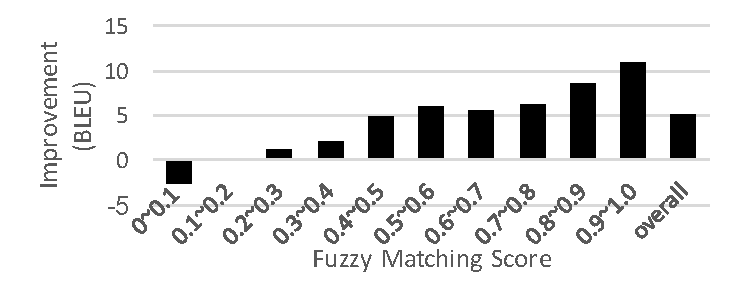
\includegraphics[width=\linewidth,clip=True,trim=0 15 0 30]{figs/seg/fuzzy_improv.pdf}
\caption{
\label{cp4.fig.fuzzy_improv}
The improvement over the baseline by SEG-NMT on Fr$\to$En w.r.t. the fuzzy matching scores of one retrieved translation pair. 
}
\end{figure}
\begin{figure}
%\vspace{-5pt}
\centering
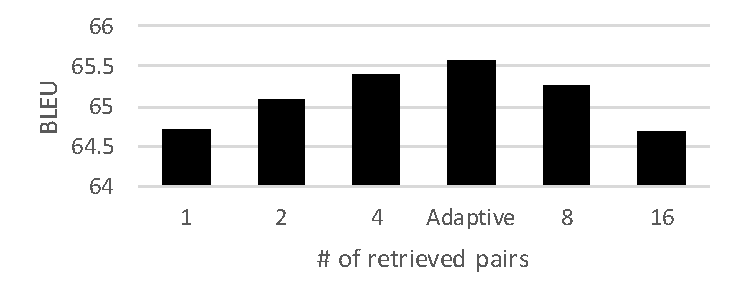
\includegraphics[width=\linewidth,clip=True,trim=0 5 0 20]{figs/seg/bleu_retrieved.pdf}
\caption{
\label{cp4.fig.bleu_retrieved}
The BLEU scores on Fr$\to$En using varying numbers of retrieved translation pairs during testing. The model was trained once. ``Adaptive'' refers to the proposed greedy selection in Alg.~\ref{cp4.algo.alg1}.
}
\end{figure}

\paragraph{Effect of the \# of Retrieved Translation Pairs}
Once the proposed model is trained, it can be used with a varying number of retrieved translation pairs. We test the model trained on Fr$\to$En with different numbers of retrieved translation pairs, and present the BLEU scores in Fig.~\ref{cp4.fig.bleu_retrieved}. We notice that the translation quality increases as the number of retrieved pairs increase up to approximately four, but from there on it degrades. We believe this happens as the retrieved sentences become less related to the current source sentence. The best quality was achieved when the proposed greedy selection algorithm in Alg.~\ref{cp4.algo.alg1} was used, in which case 4.814 translation pairs were retrieved on average. 

\paragraph{Deep vs. Shallow Fusion}
On both directions of En-Fr, we implemented and tested both deep and shallow fusion (Eqs.~\eqref{cp4.eq.deep}--\eqref{cp4.eq.shallow}) for incorporating the information from the retrieved translation pairs. With deep fusion only, the BLEU scores on the development set improved over the baseline by 1.30 and 1.20 respectively, while the improvements were 5.21 and 4.95, respectively. This suggests that the proposed model effectively exploits the availability of target symbols in the retrieved translation pairs. All other experiments were thus done using shallow fusion only.

\paragraph{Examples}
We list two good examples and one in which the proposed method makes a mistake, in Fig.~\ref{cp4.fig.examples}. From these examples, we see that the proposed SEG-NMT selects a term or phrase used in a retrieved pair whenever there are ambiguities or multiple correct translations. For instance, in the first example, SEG-NMT translated ``pr\'ecis'' into ``exact'' which was used in the retrieved pair, while the baseline model chose ``precise''. A similar behavior is found with ``examen'' in the second example. This behavior helps the proposed SEG-NMT generate a translation of which style and choice of vocabulary match better with translations from a training corpus, which improves the overall consistency of the translation.

\begin{figure}[htpb]
\centering
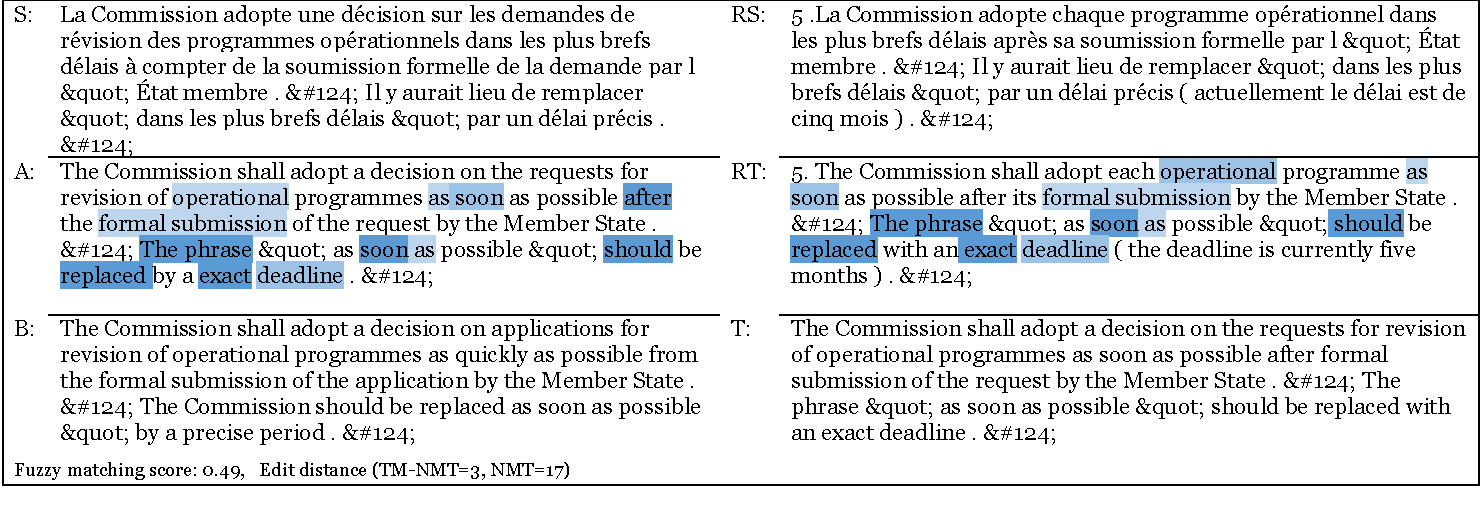
\includegraphics[width=\linewidth]{figs/seg/example-c2.pdf}
%\vspace{-1mm}
\centering
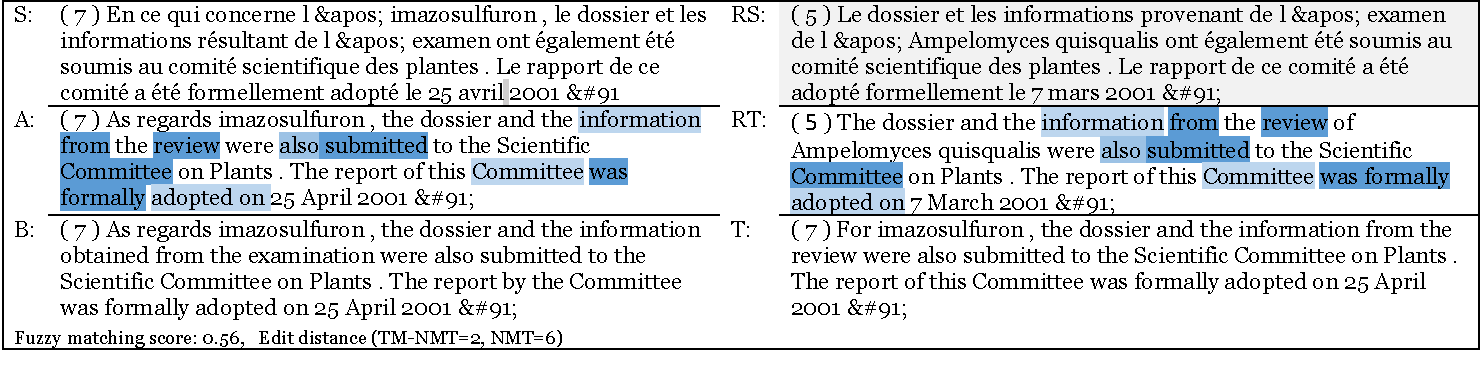
\includegraphics[width=\linewidth]{figs/seg/example-d2.pdf}
%\vspace{-1mm}
\centering
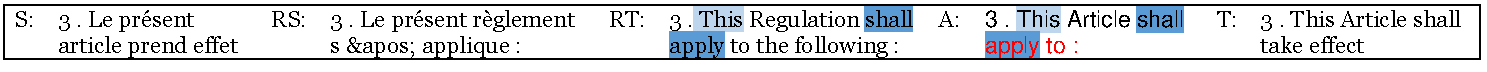
\includegraphics[width=\linewidth]{figs/seg/example-g3.pdf}
%\end{minipage}
%\caption{\label{fig.example} Examples}
%\vspace{0mm}
\caption{\label{cp4.fig.examples} 
Three examples from the Fr$\to$En test set. For the proposed SEG-NMT model, one translation pair is retrieved from the training set. Each token in the translation by the proposed approach and its corresponded token (if it exists) in the retrieved pair are shaded in blue according to the gating variable $\zeta_t$ from Eq.~\eqref{cp4.eq.shallow}. In all, we show: (S) the source sentence. (RS) the source side of a retrieved pair. (RT) the target side of the retrieved pair.
(A) the translation by the proposed approach. (B) the translation by the baseline. (T) the reference translation.
}
\end{figure}

\paragraph{Efficiency}
In general, there are two points at which computational complexity increases. The first point occurs at the retrieval stage which incurs almost no overhead as we rely on an efficient search engine (which retrieves a pair within several milliseconds.) In the translation stage, the complexity of indexing the key-value memory grows w.r.t. the \# of tokens in the retrieved pairs. This increase is however constant with a reasonably-set max \# of retrieved pairs. Note that the memory can be pre-populated for all the training pairs.

\section{Related Work}

The principal idea of SEG-NMT shares major similarities with the example-based machine translation (EBMT)~\citep{Zhang2005AnEP,callison2005scaling,phillips2012modeling} which indexes parallel corpora with suffix arrays and retrieves translations on the fly at test time. However, to the best of our knowledge, SEG-NMT is the first work incorporating any attention-based neural machine translation architectures and can be trained end-to-end efficiently, showing superior performance and scalability compared to the conventional statistical EBMT. 


% \paragraph{Multilingual neural machine translation}
%\vspace{-2mm}
SEG-NMT has also been largely motivated by recently proposed multilingual attention-based neural machine translation models~\citep{firat2016multi,zoph2016multi}. Similar to these multilingual models, our model takes into account more information than a current source sentence. This allows the model to better cope with any uncertainty or ambiguity arising from a single source sentence. More recently, this kind of larger context translation has been applied to cross-sentential modeling, where the translation of a current sentence is done with respect to previous sentences~\citep{jean2017does,wang2017exploiting}. 

% \paragraph{Nearest-neighbour image caption generation}

\newcite{devlin2015exploring} proposed an automatic image caption generation model based on nearest neighbours. In their approach, a given image is queried against a set of training pairs of images and their corresponding captions. They then proposed to use a median caption among those nearest neighboring captions, as a generated caption of the given image. This approach shares some similarity with the first stage of the proposed SEG-NMT. However, unlike their approach, we {\it learn to generate} a sentence rather than simply choose one among retrieved ones. 

% \paragraph{Large-scale question-answering}

\newcite{bordes2015large} proposed a memory network for large-scale simple question answering using an entire Freebase~\citep{bollacker2008freebase}. The output module of the memory network used simple $n$-gram matching to create a small set of candidate facts from the Freebase. Each of these candidates was scored by the memory network to create a representation used by the response module. This is similar to our approach in that it exploits a black-box search module ($n$-gram matching) for generating a small candidate set. 

% \paragraph{Neural episodic control}

%The proposed method makes the attention-based neural machine translation model non-parametric by incorporating a key-value memory that stores a training set.%
A similar approach was proposed for deep reinforcement learning by \newcite{pritzel2017neural}, where they store pairs of observed state and the corresponding (estimated) value in a key-value memory to build a non-parametric deep Q network. We consider it as a confirmation of the general applicability of the proposed approach to a wider array of problems in machine learning.
In the context of neural machine translation, \newcite{kaiser2017learning} also proposed to use an external key-value memory to remember training examples in the test time. Due to the lack of efficient search mechanism, they do not update the memory jointly with the translation model, unlike the proposed approach in this paper.

One important property of the proposed SEG-NMT is that it relies on an external, black-box search engine to retrieve relevant translation pairs. Such a search engine is used both during training and testing, and an obvious next step is to allow the proposed SEG-NMT to more intelligently query the search engine, for instance, by reformulating a given source sentence. Recently, \newcite{nogueira2017task} proposed task-oriented query reformulation in which a neural network is trained to use a black-box search engine to maximize the recall of relevant documents, which can be integrated into the proposed SEG-NMT. We leave this as future work.

%\vspace{-3mm}
\section{Conclusion and Next Chapter}
%\vspace{-3mm}

We proposed a practical, non-parametric extension of attention-based neural machine translation by utilizing an off-the-shelf, black-box search engine for quickly selecting a small subset of training translation pairs. The proposed model, called SEG-NMT, then learns to incorporate both the source- and target-side information from these retrieved pairs to improve the translation quality. We empirically showed the effectiveness of the proposed approach on the JRC-Acquis corpus using six language pair-directions. 

Although the proposed approach is in the context of machine translation, it is generally applicable to a wide array of problems. By embedding an input of any modality into a fixed vector space and using approximate search\citep{FAISS}, this approach can, for instance, be used for open-domain question answering, where the seamless fusion of multiple sources of information retrieved by a search engine is at the core. We leave these as future work.

The proposed SEG-NMT can nicely ease the data-inefficiency problem in traditional neural machine translation, especially in domains with many professional expressions that are difficult for NMT to learn but easy to copy over from similar translations. 	In principle, SEG-NMT  can be seen as a natural extension of the previously proposed \copynet (Chapter~\ref{copy}) for solving the data-inefficient problem in NMT.  However, there still exist cases that the traditional NMT is impossible to learn while SEG-NMT are also difficult to apply. For instance, when we are tackling on translation for low-resource languages. In such situations, we do not have enough ``data'' to search and copy from. In the next chapter, we will discuss one way which can greatly help to solve the data-inefficiency issue for extremely low resource languages.




\chapter[Universal Neural Machine Translation]{Universal Neural Machine Translation for Extremely Low Resource Languages}
\label{ulr}
\section{Overview}
Neural Machine Translation (NMT)~\cite{bahdanau2014neural} has achieved remarkable  translation quality in various  on-line large-scale systems~\cite{wu2016google,devlin:2017:EMNLP2017} as well as achieving  state-of-the-art results on Chinese-English  translation~\cite{hassan-hp}. With such large systems, NMT showed that it can scale up to immense  amounts of parallel data in the order of tens of millions of sentences. However, such data is not widely available for all language pairs and  domains. In this chapter, we propose a novel universal multi-lingual NMT approach  focusing mainly on low resource languages to overcome the  limitations of NMT and leverage the capabilities of multi-lingual NMT  in such scenarios.

Our approach utilizes multi-lingual neural translation system to share lexical and sentence level representations across multiple source languages into one target language. In this setup, some of the source languages may be of extremely limited  or even zero data.  The lexical sharing is represented by a  universal word-level representation where various words from all source languages  share the same underlaying representation. The sharing module utilizes monolingual embeddings along with seed parallel data from all languages to build the universal representation. The sentence-level sharing is represented by a model of language experts which  enables low-resource  languages to  utilize the sentence representation of the higher resource languages.  This allows the system to translate from any language even with tiny amount of parallel resources.  %The sentence-level sharing is represented by a model of experts from all source languages that shares the source encoders with all  other languages, this enables the low-resource  language to  utilize the sentence representation of the higher resource languages. 

We evaluate the proposed approach on 3 different  languages with tiny or even zero parallel data.
We show that for the simulated ``zero-resource" settings, our model can consistently outperform a strong multi-lingual NMT baseline with a tiny amount of parallel sentence pairs.


\section{Motivation: Low-Resource NMT}
%\subsection {Multi-Lingual NMT}
%Neural Machine Translation
%(NMT)~\cite{bahdanau2014neural,sutskever2014sequence}  is based on Sequence-to-Sequence encoder-decoder model along with an attention mechanism to enable better  handling of  longer sentences \cite{bahdanau2014neural}. Attentional sequence-to-sequence models are modeling the log conditional probability of the translation $Y$ given an input sequence $X$.  
%In general, the NMT system $\theta$ consists of two components: an encoder $\theta_e$ which transforms the input sequence into an array of continuous representations,
%and a decoder $\theta_d$ that dynamically reads the encoder's output with an attention mechanism and predicts the distribution of each target word. 
%Generally, $\theta$ is trained to maximize the likelihood on a training set consisting of $N$ parallel sentences: 
%\begin{equation}
%	\begin{split}
%	&\mathcal{L}\left(\theta\right)=\frac{1}{N}\sum_{n=1}^N\log p\left(Y^{(n)}|X^{(n)}; \theta\right) \\
%    &=\frac{1}{N}\sum_{n=1}^N\sum_{t=1}^T\log p\left(y_t^{(n)}|y_{1:t-1}^{(n)}, f^{\text{att}}_t(h^{(n)}_{1:T_s})\right)
%	\end{split}
%	 \label{eq.loss} 
%\end{equation}
%where at each step, $f^{\text{att}}_t$ builds the attention mechanism over the encoder's output $h_{1: T_s}$.
%More precisely, let the vocabulary size of source words as $V$
%\begin{equation}
%%h_{1: T_s} = f^{\text{ext}}\left[E^I(x_1),..., E^I(x_{T_s}) \right]
%h_{1: T_s} = f^{\text{ext}}\left[e_{x_1},..., e_{x_{T_s}} \right], \ \ \ e_x = E^I(x)
%\label{eq.encoder}
%\end{equation}
%where $E^I \in \mathbb{R}^{V \times d}$ is a look-up table of source embeddings, assigning each individual word a unique embedding vector; $f^{\text{ext}}$ is a sentence-level feature extractor and is usually implemented by a multi-layer bidirectional RNN~\cite{bahdanau2014neural,wu2016google}, recent efforts also achieved the state-of-the-art using non-recurrence $f^{\text{ext}}$, e.g. ConvS2S~\cite{gehring2017convolutional}  and Transformer~\cite{vaswani2017attention}.
% \begin{table}\small
%     \begin{tabular}{l|lllll}
%     \# of Sentences & 0k & \textbf{6k}  & \textbf{13k}   & 60k    & 600k   \\\hline
%     BLEU scores     & 0 & \textbf{1.21} & \textbf{2.45}  & 12.49 & 28.34 \\
%     \end{tabular}
%     \caption{\label{cp5.fig.data_size} BLEU scores reported on the test set for Ro-En. The amount of training data effects the translation performance dramatically using a single NMT model.}\vspace{-10pt}
% \end{table}


%\paragraph{Low-Resource NMT} 
Neural machine translation (NMT) $\theta$  should be trained to converge using parallel training examples (details introduced in Chapter~\ref{background}). However, the performance is highly correlated with the amount of training data.  As shown in Figure.~\ref{cp5.fig.data_size}, the system cannot achieve reasonable translation quality when the number of parallel examples is extremely small ($N \approx 13k$ sentences,  or not available at all $N =0$).  Inferior performance was also reported in the challenges noted by \newcite{koehn2017six}.

\begin{figure}[hptb]
	\centering
	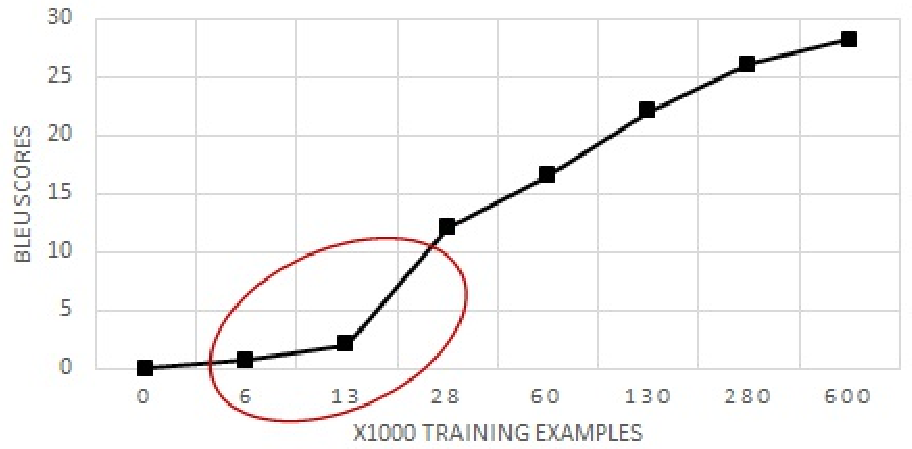
\includegraphics[width=0.85\linewidth]{figs/ulr/data_matters.pdf}
\caption{\label{cp5.fig.data_size} BLEU scores reported on the test set for Ro-En. The amount of training data effects the translation performance dramatically using a single NMT model.}
 \end{figure}

% NMT is known to easily over-fit and result in an
In general, there are two ways for handling the problem of low resource translation: (1) utilizing the resource of unlabeled monolingual data, and (2) sharing the knowledge between low- and high-resource language pairs. Many research efforts have been spent on incorporating the monolingual corpora into machine translation, such as multi-task learning~\citep{Gulcehre-Orhan-et-al-2015,zhang2016exploiting}, back-translation~\citep{sennrich2015improving}, dual learning~\citep{he2016dual} and unsupervised machine translation with monolingual corpora only~\citep{artetxe2017unsupervised,lample2017unsupervised,yang2018unsupervised}. 
%By doing so, it is usually assumed the translation pairs share similar semantic information for alignment discovered from monolingual data. 

\subsection{Multi-lingual NMT}
Prior researches attempts to exploit the knowledge of auxiliary translations, or even auxiliary tasks. For instance, \citet{cheng2016neural,chen2017teacher,lee2017emergent,chen2018zero} investigate the use of a pivot to build a translation path between two languages even without any directed resource. The pivot can be a third language or even an image in multimodal domains. When pivots are not easy to obtain, \citet{firat2016multi,lee2016fully,johnson2016google} have shown that the structure of NMT is suitable for multilingual translation. %\citet{gu2018universal} also showed that such a multilingual NMT system could improve the performance of low resource translation by using a universal lexical representation to share embedding information across languages. 
% KC: contradictory with the last sentence of this paragraph.
% It showed improvement for extremely low resource languages, e.g., with only several thousand sentences. 
%All the previous work for multilingual NMT assume the joint training of multiple high-resource languages naturally results in a universal space (for both the input representation and the model) which, however, is not necessarily true, especially for very low resource cases. 
%\newcite{lee2016fully} and \newcite{johnson2016google} have shown that NMT is quite efficient for  multilingual machine translation. 
Assuming the translation from $K$ source languages into one target language, a  system is trained with maximum likelihood on the mixed parallel pairs $\{X^{n, k}, Y^{n, k}\}_{k=1 ... K}^{n=1 ... N_k}$, that is
\begin{equation}
   %\mathcal{L}^{\text{ML}}(\theta)  = \frac{1}{N} \sum_{n=1}^N \sum_{t=1}^{T_n+1} \log p(y_t^n| y_{0:t-1}^n, x_{1:T'}^n; \theta),
	\mathcal{L}^{\text{Multi-ML}}\left(\theta\right)=\frac{1}{N}\sum_{k=1}^{K}\sum_{n=1}^{N_k} \sum_{t=1}^{T_{n, k}+1} \log p(y_t^{n,k}| y_{0:t-1}^{n,k}, x_{1:T'_{n,k}}^{n,k}; \theta),
	%^{N_k}\log p\left(Y^{(n, k)}|X^{(n, k)}; \theta\right)
\end{equation}
where $N=\sum_{k=1}^K N_k$. As the input layer, the system assumes a vocabulary which is usually the union of all  source language vocabularies with a total size as $V=\sum_{k=1}^K V_k$. In practice, it is essential to shuffle the multilingual sentence pairs into mini-batches so that different languages can be trained equally.
%% DO THEY REALLY MENTIONED ALLPOINTS BELOW??

Multi-lingual NMT is quite appealing for low-resource languages; several papers highlighted  the characteristic that make it a good fit for that  such as  \newcite{lee2016fully}, \newcite{johnson2016google}, \newcite{zoph2016transfer} and \newcite{firat2016multi}. Multi-lingual NMT utilizes the training examples of multiple languages to regularize the models  avoiding over-fitting to the limited data of the smaller languages. Moreover, the model transfers the translation knowledge from high-resource languages to low-resource ones. Finally, the decoder part of the model is sufficiently trained  since it shares  multilingual examples from all languages.
% \begin{itemize}
% \vspace{-4pt}
% \item the multilingual examples regularize the models to avoid over-fitting to the limited data;\vspace{-4pt}
% \item the decoder part is sufficiently trained  since it shares  multilingual examples;\vspace{-4pt}
% \item the model transfers translation knowledge from high-resource languages to low-resource ones. For instance, identical multilingual sentences with similar sentence structures can produce close representations from the shared encoder.\vspace{-4pt} 
% \end{itemize}
%Similar conclusions can also explained in the context of transfer learning from a pre-trained model of a high-resource %language~\cite{zoph2016transfer}.

\subsection{Challenges}
% \begin{figure}[t]
% 	\centering
% 	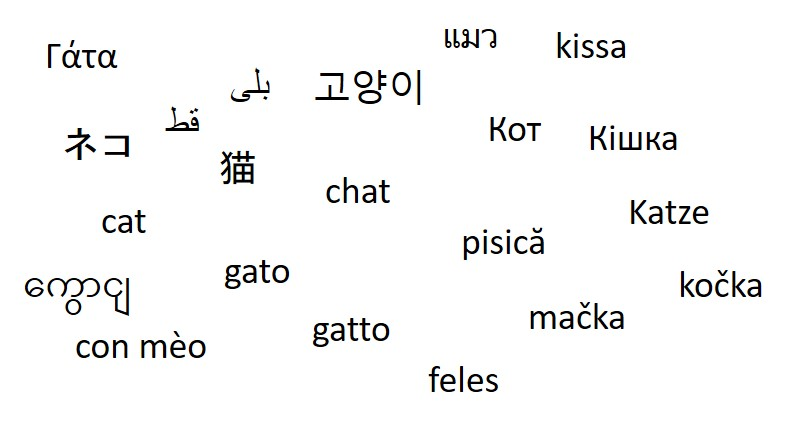
\includegraphics[width=0.9\linewidth]{figs/ulr/cat.jpg}\vspace{-15pt}
%     \caption{\label{fig.cat}word ``cat'' in different languages}\vspace{-8pt}
% \end{figure}
Despite the success of training multi-lingual NMT systems; there are a couple of challenges to leverage them for extremely low resource languages:

\paragraph{Lexical-level Sharing} Conventionally, a multi-lingual NMT model has a vocabulary that represents the union of the vocabularies of all source languages. Therefore, the multi-lingual words do not practically share the same embedding space since each word has its own representation. This does not pose a problem for languages  with sufficiently large amount of  data, yet it is a major limitation for extremely low resource languages since most of the vocabulary items will not have enough, if any, training examples to get a reliably trained models.

 \begin{figure}[hptb]
 	\centering
 	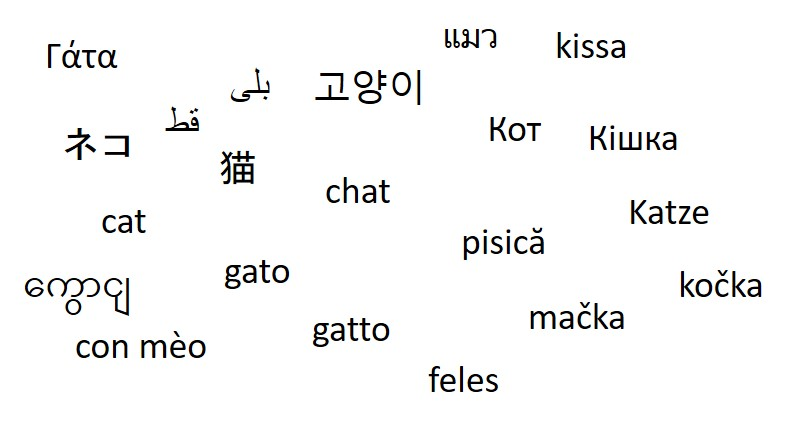
\includegraphics[width=0.85\linewidth]{figs/ulr/cat.jpg}
     \caption{\label{cp5.fig.cat}word ``cat'' in different languages}
 \end{figure}

A possible solution is to share the surface form of  all source languages through sharing sub-units such as subwords ~\cite{sennrich2015neural} or characters~\cite{kim2016character,luong2016achieving,lee2016fully}.  %However,  low-resource languages, that is not lexically quite similar to other languages, will not share surface forms with such languages . It is more crucial in such cases to have a more shared semantic representation across all languages that would enable learning translation for never seen surface forms of a given language given its semantic similarity to other  words in various languages. 
However, for an arbitrary low-resource language we cannot assume significant overlap in the lexical surface forms compared to the high-resource languages. The low-resource language may not even share the same character set as any high-resource language, e.g. as shown in Figure~\ref{cp5.fig.cat}. It is crucial to create a shared semantic representation across all languages that does not rely on surface form overlap.



\paragraph{Sentence-level Sharing} It is also crucial for low-resource languages to share source sentence representation with other similar languages. For example, if a language shares  syntactic order with another language it should be feasible for the low-resource language to share such representation with another high recourse language. It is also important to utilize monolingual data to learn such representation since the low or zero resource language may  have monolingual resources only.


%Also, as there are no enough training examples for the target language,. it is challenging to effectively share cross-lingual knowledge from multilingual training. More precisely, it is important to share only the useful information from other languages and avoid unnecessary interference.
%In this work, the sentence-level sharing is handled basically in three considerations:\vspace{-3pt}
% \begin{itemize}
% \item choice of auxiliary languages; \vspace{-8pt}
% \item architecture easy to avoid interference; \vspace{-8pt}
% \item utilizing the monolingual data; \vspace{-3pt}
% \end{itemize}

\section{Universal Neural Machine Translation}
We propose a Universal NMT system that is focused on the scenario where minimal parallel sentences are available. 
%We propose a novel approach that enable translation using very a very small amount of parallel data, including ``Zero-Resource'' translation.
As shown in Fig.~\ref{cp5.fig.model}, we introduce two components to extend the conventional multi-lingual NMT system \cite{johnson2016google}: Universal Lexical Representation (ULR) and Mixture of Language Experts (MoLE) to enable both word-level and sentence-level sharing, respectively.
\begin{figure}[hptb]
	\centering
	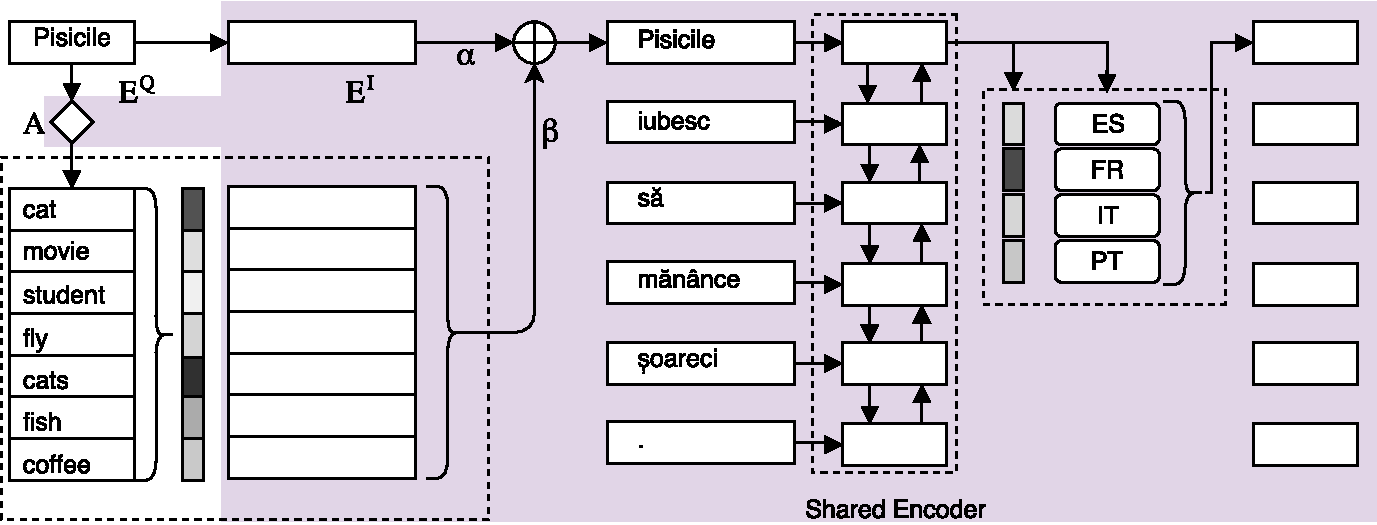
\includegraphics[width=\linewidth]{figs/ulr/model2x}
      \caption{\label{cp5.fig.model} An illustration of the proposed architecture of ULR and MoLE. Shaded parts are trained within the NMT model while unshaded parts are not changed during  training.}
  \end{figure}

\subsection{Universal Lexical Representation (ULR)}
\label{cp5.sec.unilex}

As we highlighted above, it is not straightforward to have a universal representation  for all languages. One potential approach is to use a shared source vocabulary, but this is not adequate since it assumes significant  surface-form overlap in order being able to generalize between high-resource and low-resource languages. Alternatively, we could train monolingual embeddings in a shared space and use these as the input to our MT system. However, since these embeddings are trained on a monolingual objective, they will not be optimal for an NMT objective. If we simply allow them to change during NMT training, then this will not generalize to the low-resource language where many of the words are unseen in the parallel data.
Therefore, our goal is to create a shared embedding space which (a) is trained towards NMT rather than a monolingual objective, (b) is not based on lexical surface forms, and (c) will generalize from the high-resource languages to the low-resource language. 

We propose a novel representation for multi-lingual embedding where each word from any language is represented as a probabilistic mixture of universal-space word embeddings. In this way, semantically similar words from different languages will naturally have similar representations. Our  method achieves this  utilizing a discrete (but probabilistic) ``universal token space'', and then learning the embedding matrix for these universal tokens directly in our NMT training.

\paragraph{Lexicon Mapping to the Universal Token Space}
We first define a discrete universal token set of size $M$ into which all source languages will be projected. In principle, this could correspond to any human or symbolic language, but all experiments here use English as the basis for the universal token space. As shown in Figure \ref{cp5.fig.model}, we have multiple embedding representations. $\epsilon_Q$ is language-specific embedding trained on  monolingual data and $\epsilon_K$ is universal tokens embedding. The matrices $\epsilon_K$ and $\epsilon_Q$ are created beforehand and are not trainable during NMT training.  $\epsilon_U$ is the embedding matrix for these universal tokens which is learned during  our NMT training.  It is worth noting that shaded parts in Figure\ref{cp5.fig.model} are trainable during  NMT training process.

Therefore, each source word  $x$ is represented as a mixture of universal tokens $M$ of $\epsilon_U$.
\begin{equation}
	\epsilon[x] = \sum_{i=1}^M \epsilon_U\left[u_i\right] \cdot q(u_i|x)
    \label{cp5.eq.universal_embed}
\end{equation}
where $\epsilon_U$ is an NMT embedding matrix, which is learned during NMT training.
The mapping $q$ projects the multilingual words into the universal space based on their semantic similarity. That is, $q(u|x)$ is a distribution based on the similarity between $u$ and $x$ as:
\begin{equation}
 q(u_i|x) = \ssoftmax_{u_i}\left(\epsilon_K[u]^\top \cdot A \cdot \epsilon_Q[x] / \tau \right) % \frac{e^{D(u_i, x) / \tau}}{\sum_{u_j} e^{D(u_j, x) / \tau}}
 \label{cp5.eq.q_softmax}
\end{equation}
where $\tau$ is a temperature hyper-parameter; %and $D(u_i, x)$ is a scalar score which represents the similarity between source word $x$ and universal token $u_i$:
%\begin{equation}
%\label{eq.ds}
%	D(u, x) =  E^K(u)\cdot A\cdot E^Q(x)^T
%\end{equation}
$\epsilon_K[u]$ is the ``key'' embedding of word $u$, $\epsilon_Q[x]$ is the ``query'' embedding of source word $x$.  The transformation matrix $A$, which is initialized to the identity matrix, is learned during NMT training and shared across all languages. 

%This representation can effectively represent  unlimited multi-lingual vocabulary that can represent any word that has never been observed in the parallel training data. 
This is a key-value representation, where the queries  are the monolingual language-specific embedding, the keys are the universal tokens embeddings and the values are a probabilistic distribution over the universal NMT embeddings. 
This can  represent  unlimited  multi-lingual vocabulary  that has  never been observed in the parallel training data.   
It is worth noting  that the trainable transformation matrix $A$ is added  to the query matching mechanism  with the main purpose to tune the similarity scores towards the translation task. For example, words like “autumn”, “fall”, “toamna” (autumn in Romanian)  and  “spring” would be quite similar from the monolingual embedding view while  “spring” should be less similar for the translation  task. 
$A$ is shared across all languages and optimized discriminatively during NMT training such that the system can fine-tune the similarity score $q(\cdot)$ to be optimal for NMT.

%For example, words like “autumn”, “fall”, “toamna” (means autumn in Romanian)  and  “spring” would be quite similar from the monolingual embedding view while  “spring” should be less similar for the translation  task. 

% JIATAO, review above: where $E^K(u)$ is the ``key'' embedding of word $u$, $E^V(x)$ is the ``value'' embedding of source word $x$. The transformation matrix $A$, which is initialized to the identity matrix, is learned during NMT training and shared across all languages. The matrices $E^K$ and $E^Q$ are created beforehand and do not change during NMT training. We next describe how these matrices are created.

\paragraph{Shared Monolingual Embeddings}
In general, we create one $\epsilon_Q$ matrix per source language, as well as a single $\epsilon_K$ matrix in our universal token language. For Eq.~\eqref{cp5.eq.universal_embed} to make sense and generalize across language pairs, all of these embedding matrices must live in a similar semantic space. To do this, we first train off-the-shelf monolingual word embeddings in each language, and then learn one projection matrix per source language which maps the original monolingual embeddings into $\epsilon_K$ space.
Typically, we need a list of \textit{source - universal token} pairs (seeds $S_k$) to train the projection matrix for language $k$. Since vectors are normalized, learning the optimal projection is equivalent to finding an orthogonal transformation $O_k$ that makes the projected word vectors as close as to its corresponded universal tokens:
\begin{equation}
  \begin{array}{l}  
         \max\limits_{O_k}\mathlarger{\sum}\limits_{(\tilde{x}, \tilde{y})\in S_k}  \epsilon_{Q_k}[\tilde{x}]^\top \cdot O_k \cdot \epsilon_K[\tilde{y}] \\  
         \text{s.t.       } O_k^\top O_k = I, \ \ \ k=1, ..., K
 \end{array}  
\end{equation}
which can be solved by SVD decomposition based on the seeds~\cite{smith2017offline}. We chose to use a short list of seeds from automatic word-alignment of parallel sentences  to learn the projection. However, recent efforts~\cite{Artetxe2017LearningBW,Conneau2017WordTW}   also showed that it is possible to learn the transformation without any seeds, which makes it feasible  for our  proposed method to be utilized in purely zero parallel resource cases.
It is worth noting that  $O_k$ is a language-specific matrix which maps the monolingual embeddings of each source language into a similar semantic space as the universal token language.

\begin{figure}[hptb]
	\centering
	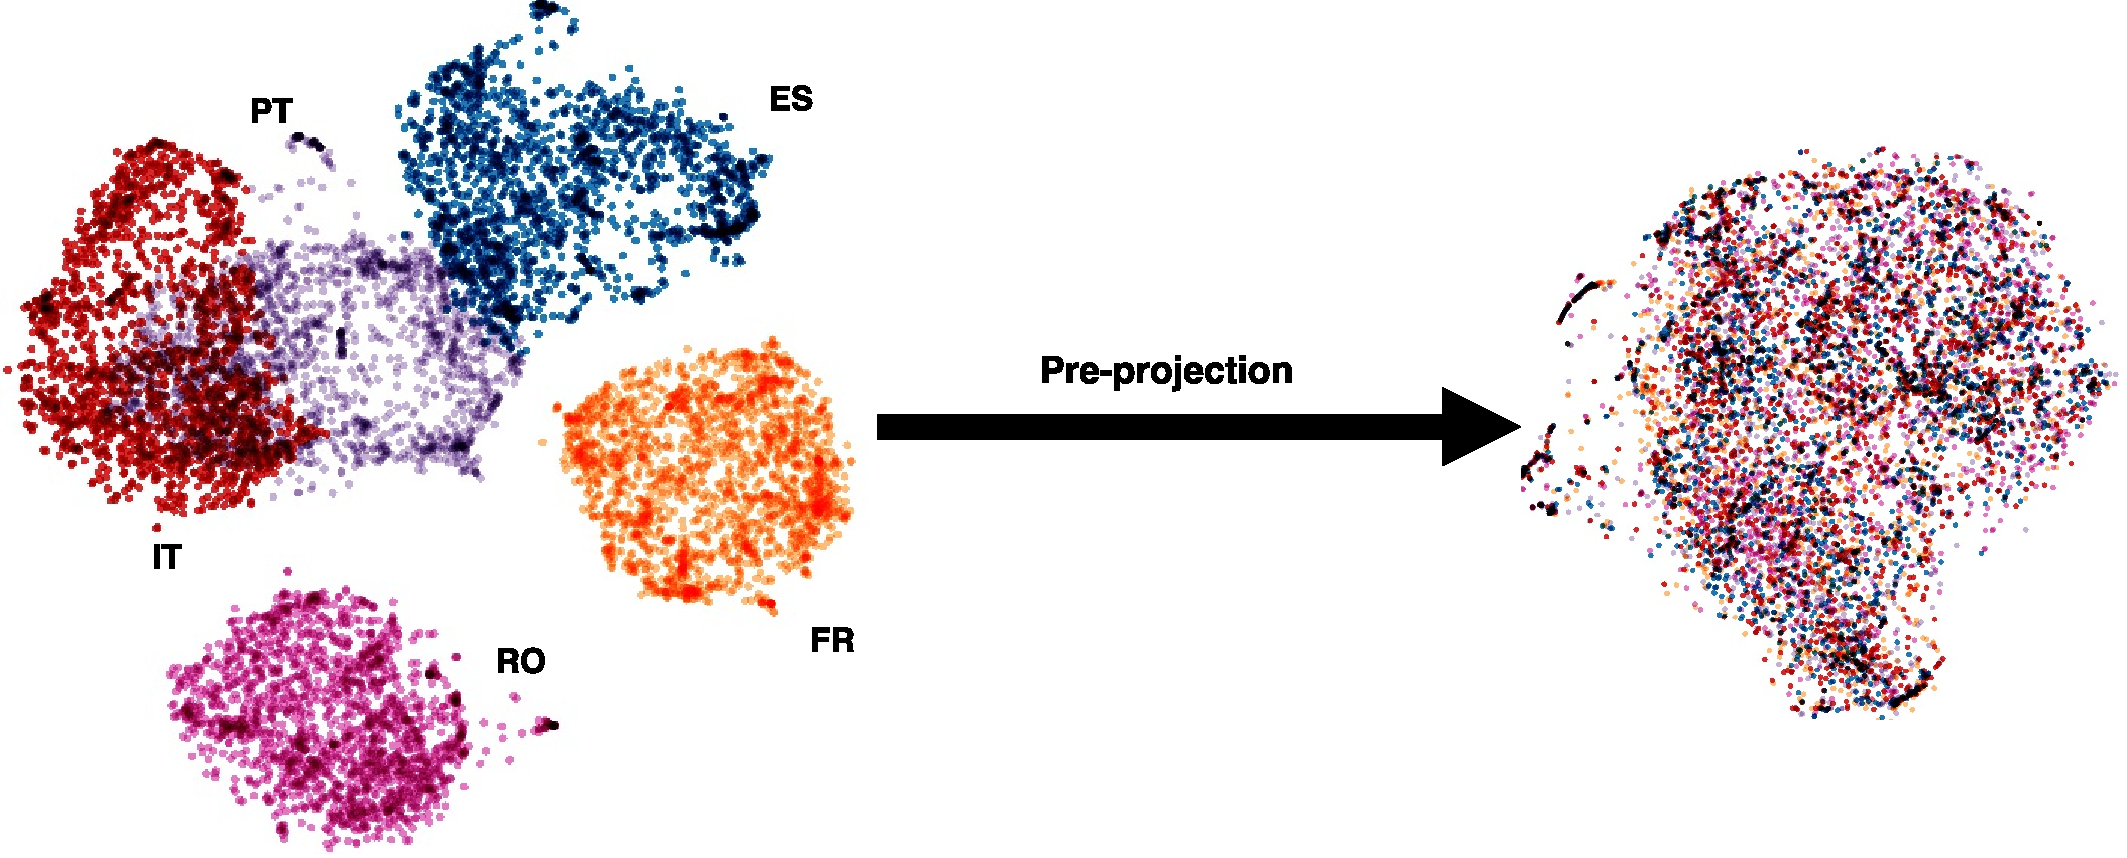
\includegraphics[width=\linewidth]{figs/ulr/preprojection}
      \caption{\label{cp5.fig.preproj} An illustration of projecting multiple monolingual embeddings (Es, Fr, It, Pt, Ro) to the same universal (En) space.}
  \end{figure}

%$A$ is shared across all languages and optimized discriminatively during NMT training. Empirically we have found that removing $A$ hurts performance by up to 3 BLEU points, as the system cannot fine-tune the similarity score $q()$ to be optimal for NMT.

\paragraph{Interpolated Embeddings}
Certain lexical categories (e.g. function words) are poorly captured by Eq.~\eqref{cp5.eq.universal_embed}. Luckily, function words often have very high frequency, and can be estimated robustly from even a tiny amount of data. This motivates an interpolated $\epsilon[x]$ where embeddings for very frequent words are optimized directly and  not through the universal tokens:
\begin{equation}
	\epsilon[x] = \alpha(x) \cdot \epsilon_E[x] + \beta(x) \cdot \sum_{i=1}^M \epsilon_U[u_i] \cdot q(u_i|x),
\end{equation}
where $\epsilon_E[x]$ is a language-specific embedding of word $x$ (as discussed in Chapter ~\ref{background}), which is optimized during NMT training. In general, we set $\alpha(x)$ to 1.0 for the top 500 most frequent words in each language, and 0.0 otherwise. Besides, we do not use an absolute frequency cutoff because this would cause a mismatch between high-resource and low-resource languages, which we want to avoid. We keep $\beta(x)$ fixed to 1.0.

\paragraph{An Example} To give a concrete example, imagine that our target language is English (En), our high-resource auxiliary source languages are Spanish (Es) and French (Fr), and our low-resource source language is Romanian (Ro). En is also used for the universal token set. We assume to have 10M+ parallel Es-En and Fr-En, and a few thousand in Ro-En. We also have millions of monolingual sentences in each language.

We first train word2vec embeddings on monolingual corpora from each of the four languages. We next align the Es-En, Fr-En, and Ro-En parallel corpora and extract a seed dictionary of a few hundred words per language, e.g., ${\tt gato} \rightarrow {\tt cat}$,  ${\tt chien} \rightarrow {\tt dog}$. We then learn three matrices $O_1, O_2, O_3$ to project the Es, Fr and Ro embeddings ($\epsilon_{Q_1}, \epsilon_{Q_2}, \epsilon_{Q_3}$), into En ($\epsilon_K$) based on these seed dictionaries. At this point, Eq.~\eqref{cp5.eq.q_softmax} should produce \textit{reasonable} alignments between the source languages and En, e.g., $q(\tt{horse}|\tt{magar}) = 0.5$, $q(\tt{donkey}|\tt{magar}) = 0.3$, $q(\tt{cow}|\tt{magar}) = 0.2$, where {\tt magar} is the Ro word for {\tt donkey}. %Therefore, any word can be represented as  a probabilistic mixture of universal tokens.

\subsection{Mixture of Language Experts (MoLE)}
\label{cp5.sec.moe}
As we paved the road for having a universal embedding representation; it is crucial to have a  language-sensitive module for the encoder that would help in modeling various  language structures which may  vary between different languages. 
We propose a Mixture of Language Experts (MoLE) to model the sentence-level universal encoder. As shown in Fig.~\ref{cp5.fig.model}, 
an additional module of mixture of experts is used after the last layer of the encoder. Similar to \cite{shazeer2017outrageously}, we have a set of expert networks and a gating network  to control the weight of each expert. More precisely, we have a set of expert networks as $f_1(h), ..., f_{K}(h)$ where for each expert, a two-layer feed-forward network which reads the output encoder hidden states $h$ for each word. The output of the MoLE module $h'$ will be a weighted sum of these experts to replace the encoder's representation:
\begin{equation}
s'=\sum_{k=1}^K f_k(h)\cdot \ssoftmax_{k}(g(h)_k),
\end{equation}
where an one-layer feed-forward network $g(h)_k$ is used as a gate to compute score for the  $k$-th expert.

In our case, we create one expert per auxiliary language. In other words, we train to only use expert $f_i$ when training on a parallel sentence from auxiliary language $i$. Assume the language $1 ... K-1$ are the auxiliary languages. That is, we have a multi-task objective:
\begin{equation}
\begin{split}
\mathcal{L}^{\text{gate}} = \frac{1}{N'}\sum_{k=1}^{K-1}\sum_{n=1}^{N_k}\sum_{\tau=1}^{T'_{n, k}}\log \left[\ssoftmax_{k}\left(g(h^{n, k}_\tau)_k\right)\right],
\end{split}
\end{equation}
where $N'=\sum_{k=1}^{K-1}N_k$. We do not update the MoLE module for training on a sentence from the low-resource language. Intuitively, this allows us to represent each token in the low-resource language as a context-dependent mixture of the auxiliary language experts.

% Note that, in our cases, we only assign the experts for the auxiliary languages so that each language will try to optimize its own expert.


\section{Experiments}
\label{cp5.sec.exps}
We extensively study the effectiveness of the proposed methods by evaluating on three (simulated) extremely low-resource language pairs with variant auxiliary languages. The vanilla single-source NMT and the multi-lingual NMT models are used as baselines.
\subsection{Settings}
%\paragraph{Dataset} We empirically evaluate the proposed \textsc{ZR-NMT} on $4$ languages -- Romanian (Ro) / Latvian (LV) / Korean (KO) / Levantine Arabic (LEV)\footnote{A spoken dialect of standard Arabic.} -- translating to English (En) in near zero-resource settings. To achieve this, single or multiple auxiliary languages from Czech (Cs), German (De), Greek (El), Spanish (Es), Finnish (Fi), French (Fr),  Italian (It), Portuguese (Pt), Russian (Ru) and Modern Standard Arabic (MSA) are jointly trained to translate to English.

\paragraph{Dataset} We empirically evaluate the proposed Universal NMT system on $3$ languages -- Romanian (Ro) / Latvian (Lv) / Korean (Ko)  -- translating to English (En) in near zero-resource settings. To achieve this, single or multiple auxiliary languages from Czech (Cs), German (De), Greek (El), Spanish (Es), Finnish (Fi), French (Fr),  Italian (It), Portuguese (Pt) and Russian (Ru) are jointly trained. The detailed statistics and sources of the available parallel resource can be found in Table~\ref{cp5.table.data0} and \ref{cp5.table.data1}, where we further down-sample the corpora for the targeted languages to simulate extremely low resource. 

\begin{savenotes}
\begin{table}[hptb]
\centering
%\begin{tabular}{p{0.7cm}||*{13}{p{0.3cm}}}
\begin{tabular}{c|ccc}%{p{0.7cm}|*{4}{p{0.5cm}}}
\hline
source &  
\multicolumn{1}{c|}{Ro} & 
\multicolumn{1}{c|}{Ko} & 
\multicolumn{1}{c}{Lv}  \\ \hline
corpora & 
\multicolumn{1}{c|}{WMT16\footnote{http://www.statmt.org/wmt16/translation-task.html}} & 
\multicolumn{1}{c|}{KPD\footnote{https://sites.google.com/site/koreanparalleldata/}} &  
\multicolumn{1}{c}{Europarl v8\footnote{http://www.statmt.org/europarl/}} \\ \hline
size 
& \multicolumn{1}{c|}{612k} & \multicolumn{1}{c|}{97k} & \multicolumn{1}{c}{638k}  \\ \hline
subset & \multicolumn{1}{c|}{0/6k/60k} & \multicolumn{1}{c|}{10k} & \multicolumn{1}{c}{6k} \\ \hline
\end{tabular}
\caption{\label{cp5.table.data0}Statistics of the available parallel resource for extremely low-resource languages in our experiments. 	All are translated to English.}
\end{table}
\end{savenotes}

\begin{savenotes}
\begin{table}[hptb]
\centering
%\begin{tabular}{p{0.7cm}||*{13}{p{0.3cm}}}
\begin{tabular}{c|ccccccccc}
\hline
source &  
\multicolumn{1}{c|}{Cs} & \multicolumn{1}{c|}{De} & \multicolumn{1}{c|}{El}  & \multicolumn{1}{c|}{Es}  & \multicolumn{1}{c|}{Fi} & 
\multicolumn{1}{c|}{Fr} & \multicolumn{1}{c|}{It} & \multicolumn{1}{c|}{Pt} &  
\multicolumn{1}{c}{Ru}  \\ \hline
corpora & \multicolumn{8}{c|}{Europarl v8\footnote{http://www.statmt.org/europarl/}} & \multicolumn{1}{c}{UN \footnote{http://opus.lingfil.uu.se/MultiUN.php (we use a subset of 2M sentence pairs.)}} \\ \hline
size 
& \multicolumn{1}{c|}{645k} & \multicolumn{1}{c|}{1.91m} 
& \multicolumn{1}{c|}{1.23m} & \multicolumn{1}{c|}{1.96m} & \multicolumn{1}{c|}{1.92m} & \multicolumn{1}{c|}{2.00m} & \multicolumn{1}{c|}{1.90m} 
& \multicolumn{1}{c|}{1.96m} & \multicolumn{1}{c}{2.00m}  \\ \hline
%subset & \multicolumn{8}{c}{/} &\multicolumn{1}{|c}{2.00m}\\ \hline
\end{tabular}
\caption{\label{cp5.table.data1}Statistics of the available parallel resource in our experiments. 	All the languages are translated to English.}
\end{table}
\end{savenotes}


It also requires additional large amount of monolingual data to obtain the word embeddings for each language, where we use the latest Wikipedia dumps\footnote{https://dumps.wikimedia.org/} for all the languages. Typically, the monolingual corpora are much larger than the parallel corpora. For validation and testing, the standard validation and testing sets are utilized for each targeted language.

\paragraph{Preprocessing}
All the data (parallel and monolingual) have been tokenized and segmented into subword symbols using byte-pair encoding (BPE)~\cite{sennrich2015neural}. We use sentences of length up to 50 subword symbols for all languages.  For each language, a maximum number of $40,000$ BPE operations are  learned and  applied to restrict the size of the vocabulary.  We concatenate the vocabularies of all source languages in the multilingual setting where special a ``language marker " have been appended to each word  so that there will be no embedding sharing on the surface form. Thus, we avoid sharing the representation  of words that have similar surface forms though with different meaning in various languages.

\paragraph{Architecture} We implement an attention-based neural machine translation model which consists of a one-layer bidirectional RNN encoder and a two-layer attention-based RNN decoder. All  RNNs have 512 LSTM units~\cite{hochreiter1997long}. Both the dimensions of the source and target embedding vectors are set to 512. The dimensionality of universal embeddings is also the same. For a fair comparison, the same architecture is also utilized for training both the vanilla and multilingual NMT systems. For multilingual experiments, $1\sim 5$ auxiliary languages are used.  When training with the universal tokens, the temperature $\tau$ (in Eq.~\eqref{cp5.eq.universal_embed}) is fixed to $0.05$ for all the experiments.

\paragraph{Learning}
All the models are trained to maximize the log-likelihood using Adam~\cite{kingma2014adam} optimizer for 1 million steps on the mixed dataset with a batch size of 128. The dropout rates for both the encoder and the decoder is set to 0.4. % In general, it takes about $4$ days for learning a multilingual model of $8m$ sentences on single GTX Titan.
% HOW MANY STEPS with batch size
%\paragraph{Implementation}
%The initial experiments in this paper were conducted based on Tensorflow. 
We have open-sourced an implementation of the proposed model\footnote{https://github.com/MultiPath/NA-NMT/tree/universal\_translation}.


\subsection{Back-Translation}
We utilize back-translation (BT)~\cite{sennrich2016edinburgh} to encourage the model to use more information of the zero-resource languages. More concretely, we build the synthetic parallel corpus by translating on monolingual data\footnote{We used News Crawl provided by WMT16 for Ro-En.} with a trained translation system and use it to train a backward direction translation model. Once trained, the same operation can be used on the forward direction. 
Generally, BT is difficult to apply for zero resource setting since it requires a reasonably good translation system to generate good quality synthetic parallel data. Such a system may not be feasible with tiny or zero parallel data. However, it is possible to start with a trained multi-NMT model.

\subsection{Preliminary Experiments}
\paragraph{Training Monolingual Embeddings} We train the monolingual embeddings  over the Wikipedia corpora of all the languages using \texttt{fastText}\footnote{https://github.com/facebookresearch/fastText}~\cite{bojanowski2016enriching} .  The vectors are set to 300 dimensions, trained using the default setting of skip-gram . All the vectors are normalized to norm $1$.

\paragraph{Pre-projection} In this chapter, the pre-projection requires initial word alignments (seeds) between words of each source language and the universal tokens.  More precisely, for the experiments of Ro/Ko/Lv-En, we use the target language (En) as the universal tokens;  \texttt{fast\_align}\footnote{https://github.com/clab/fast\_align} is used to automatically collect the aligned words between the source languages and English. %Word alignment with the highest probability is picked as a seed.  

% On the other hand, for the experiments of LEV-En, MSA will be used as the universal tokens considering LEV is a dialect of MSA and it shares around 40\%  of the vocabularies with MSA. It is possible to directly use the shared words as the seeds to train the projection matrix for LEV. 
% To increase the robustness,  only words with a frequency larger than $15$ are considered. Pre-projection can be performed based on the seeds off-line and stored for NMT training.
%  ADD MORE INFO ON NUM OF SEEDS / SENTENCES
\subsection{Results}

% \begin{tabular}{c|ccccccccc|r|r|r}
% Source & Cs    & De    & El & Es & Fi & Fr & It & Pt & Ru & Multi-NMT & + UnivTok & + MoE \\ \hline
% \multirow{ 4}{*}{Ro}     
% & \Checkmark & \Checkmark & \Checkmark & ~  & \Checkmark  & ~  & ~  & ~  & ~  
% & & 18.02 & 18.37   \\
% & \Checkmark & \Checkmark & \Checkmark  & ~  & ~  & \Checkmark  & ~  & ~  & ~  
% & ~    & 19.48     &  19.52  \\
% &  & \Checkmark & \Checkmark  & ~  & \Checkmark  & ~  &  \Checkmark  & ~  & ~  
% & ~    & 19.11     & 19.33   \\
% & ~     & ~     & ~  &  \Checkmark  & ~  &  \Checkmark  &  \Checkmark  &  \Checkmark  & ~  
% & 14.83   & 20.01   &  \textbf{20.51} \\ \hline
% \multirow{ 2}{*}{LV}      
% & ~     & ~  & ~ & \Checkmark  & ~  &  \Checkmark  &  \Checkmark  &  \Checkmark  & ~  
% & 7.68     & 10.86     &  11.02 \\ 
% & ~     & ~  & ~ & \Checkmark  & ~  &  \Checkmark  &  \Checkmark  &  \Checkmark  & \Checkmark & 7.88     & 12.40     &  \textbf{13.16} \\  \hline
% KO    & ~     & ~  & ~ & \Checkmark  & ~  &  \Checkmark  &  \Checkmark  &  \Checkmark  & ~  
% & 2.45    & 5.49    & \textbf{6.14}  \\     
% \end{tabular}



We show our main results of multiple source languages to English with different auxiliary languages in Table~\ref{cp5.table.bleu}. To have a fair comparison, we use only 6k sentences corpus for both Ro and Lv with all the settings and 10k for Ko. It is obvious that applying both the universal tokens and mixture of experts modules  improve the overall translation quality for all the language pairs and the improvements are additive. 
\begin{table}[hptb]
\centering
\begin{tabular}{l|c|rrr}
Src & Aux   & Multi & +ULR & + MoLE \\ \hline
\multirow{ 4}{*}{Ro}     
& Cs De El Fi & & 18.02 & 18.37   \\
& Cs De El Fr & & 19.48 &  19.52  \\
& De El Fi It & & 19.11 & 19.33   \\
& Es Fr It Pt & 14.83   & 20.01   &  \textbf{20.51} \\ \hline
\multirow{ 2}{*}{Lv}      
& Es Fr It Pt & 7.68     & 10.86     &  11.02 \\ 
& Es Fr It Pt Ru & 7.88     & 12.40     &  \textbf{13.16} \\  \hline
Ko    & Es Fr It Pt  & 2.45    & 5.49    & \textbf{6.14}  \\     
\end{tabular}
\caption{\label{cp5.table.bleu} Scores over variant source languages (6k sentences for Ro \& Lv, and 10k for Ko). ``Multi" means the Multi-lingual NMT baseline.}
\end{table}


 \begin{figure}[hptb]
	\centering
%    \begin{minipage}[t]{0.48\textwidth}
%    \centering
    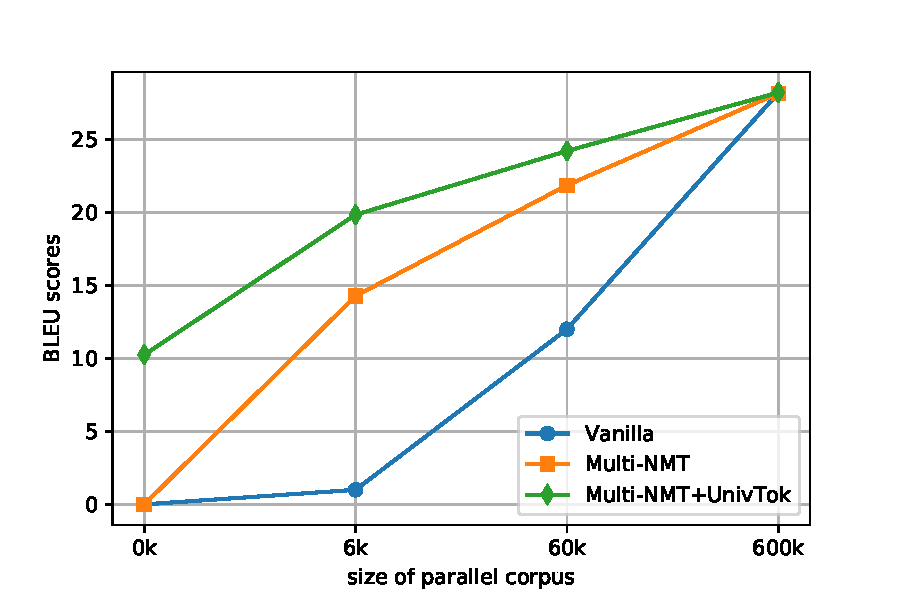
\includegraphics[width=0.85\linewidth]{figs/ulr/size} 
    \caption{\label{cp5.fig.size}BLEU score vs corpus size}
    \end{figure}
    \begin{figure}[hptb]
%    \begin{minipage}[t]{0.48\textwidth}
    \centering
    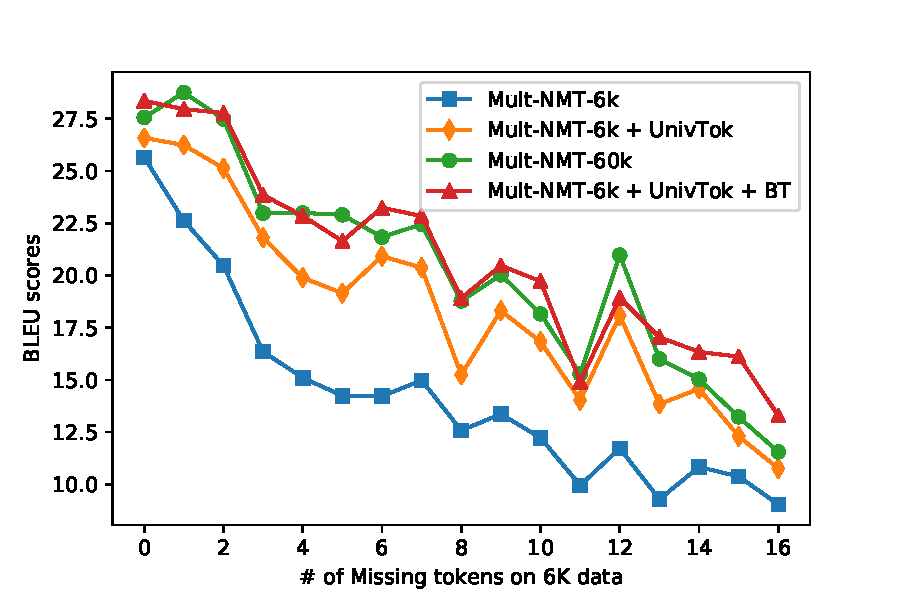
\includegraphics[width=0.85\linewidth]{figs/ulr/missing} 
    \caption{\label{cp5.fig.missing}BLEU score vs unknown tokens}
\end{figure}

To examine the influence  of auxiliary languages, we tested four sets of different combinations of auxiliary languages for Ro-En and two sets for Lv-En. It shows that Ro performs best when the auxiliary languages are all selected in the same family (Ro, Es, Fr, It and Pt are all from the Romance family of European languages) which makes sense as more knowledge can be shared across the same family. Similarly, for the experiment of Lv-En, improvements are also observed when adding Ru as additional auxiliary language as Lv and Ru share many similarities because of the geo-graphical influence even though they don't share the same alphabet. 

We also tested a set of Ko-En experiments to examine the generalization capability of our approach on  non-European languages while using languages of Romance family as auxiliary languages. Although the BLEU score is relatively low, the proposed methods can consistently help  translating less-related low-resource languages. It is more reasonable to have  similar languages as auxiliary languages.



\paragraph{Ablation Study}
We perform  thorough experiments to examine effectiveness of the proposed method; we do ablation study on Ro-En where  all the models are trained based on the same Ro-En corpus with 6k sentences.  
\begin{table}[hptb]
 	\centering
    \begin{tabular}{l|r}
    Models                   & BLEU  \\ \hline
    Vanilla                        & 1.21   \\
    Multi-NMT                 & 14.94 \\ \hline
    Closest Uni-Token Only        & 5.83  \\
    Multi-NMT + ULR + ($A$=$I$) & 18.61 \\ 
    Multi-NMT + ULR       & \textbf{20.01} \\ \hline
    Multi-NMT + BT & 17.91 \\
    Multi-NMT + ULR + BT & \textbf{22.35} \\  \hline
    Multi-NMT + ULR + MoLE & 20.51 \\
    Multi-NMT + ULR + MoLE + BT & \textbf{22.92} \\ \hline\hline
    Full data (612k) NMT & \textbf{28.34} \\
    \end{tabular}
    \caption{\label{cp5.table.ro_test1} BLEU scores evaluated on test set (6k), compared with ULR and MoLE. ``vanilla" is the standard NMT system trained only on Ro-En training set}
\end{table}

As shown in Table~\ref{cp5.table.ro_test1}, it is obvious that 6k sentences of parallel corpora  completely fails to train a vanilla  NMT model. Using Multi-NMT with the assistance of 7.8M auxiliary language sentence pairs, Ro-En translation performance gets a substantial improvement which, however, is still limited to be usable. By contrast, the proposed ULR boosts the Multi-NMT significantly with +5.07 BLEU, which is further boosted to +7.98 BLEU when incorporating sentence-level information using both MoLE and BT.  Furthermore, it is also shown that ULR works better when a trainable transformation matrix $A$ is used (4th vs 5th row in the table). Note that, although still $5\sim 6$ BLEU scores lower than the full data ($\times 100$ large) model. 

We also measure the translation quality of simply training the vanilla system while replacing each  token of the Ro sentence with its closet universal token in the projected embedding space, considering we are using the target languages (En) as the universal tokens. Although the performance is much worse than the baseline Multi-NMT, it still outperforms the vanilla model which implies the effectiveness of the embedding alignments.

\paragraph{Monolingual Data}
In Table.~\ref{cp5.table.ro_test1},  we also showed the performance when incorporating the monolingual Ro corpora to help the UniNMT training in both cases with and without ULR. The back-translation improves in both cases, while the  ULR  still obtains the best score  which indicates that the gains achieved are additive.

\begin{sidewaysfigure}[hptb]
\centering
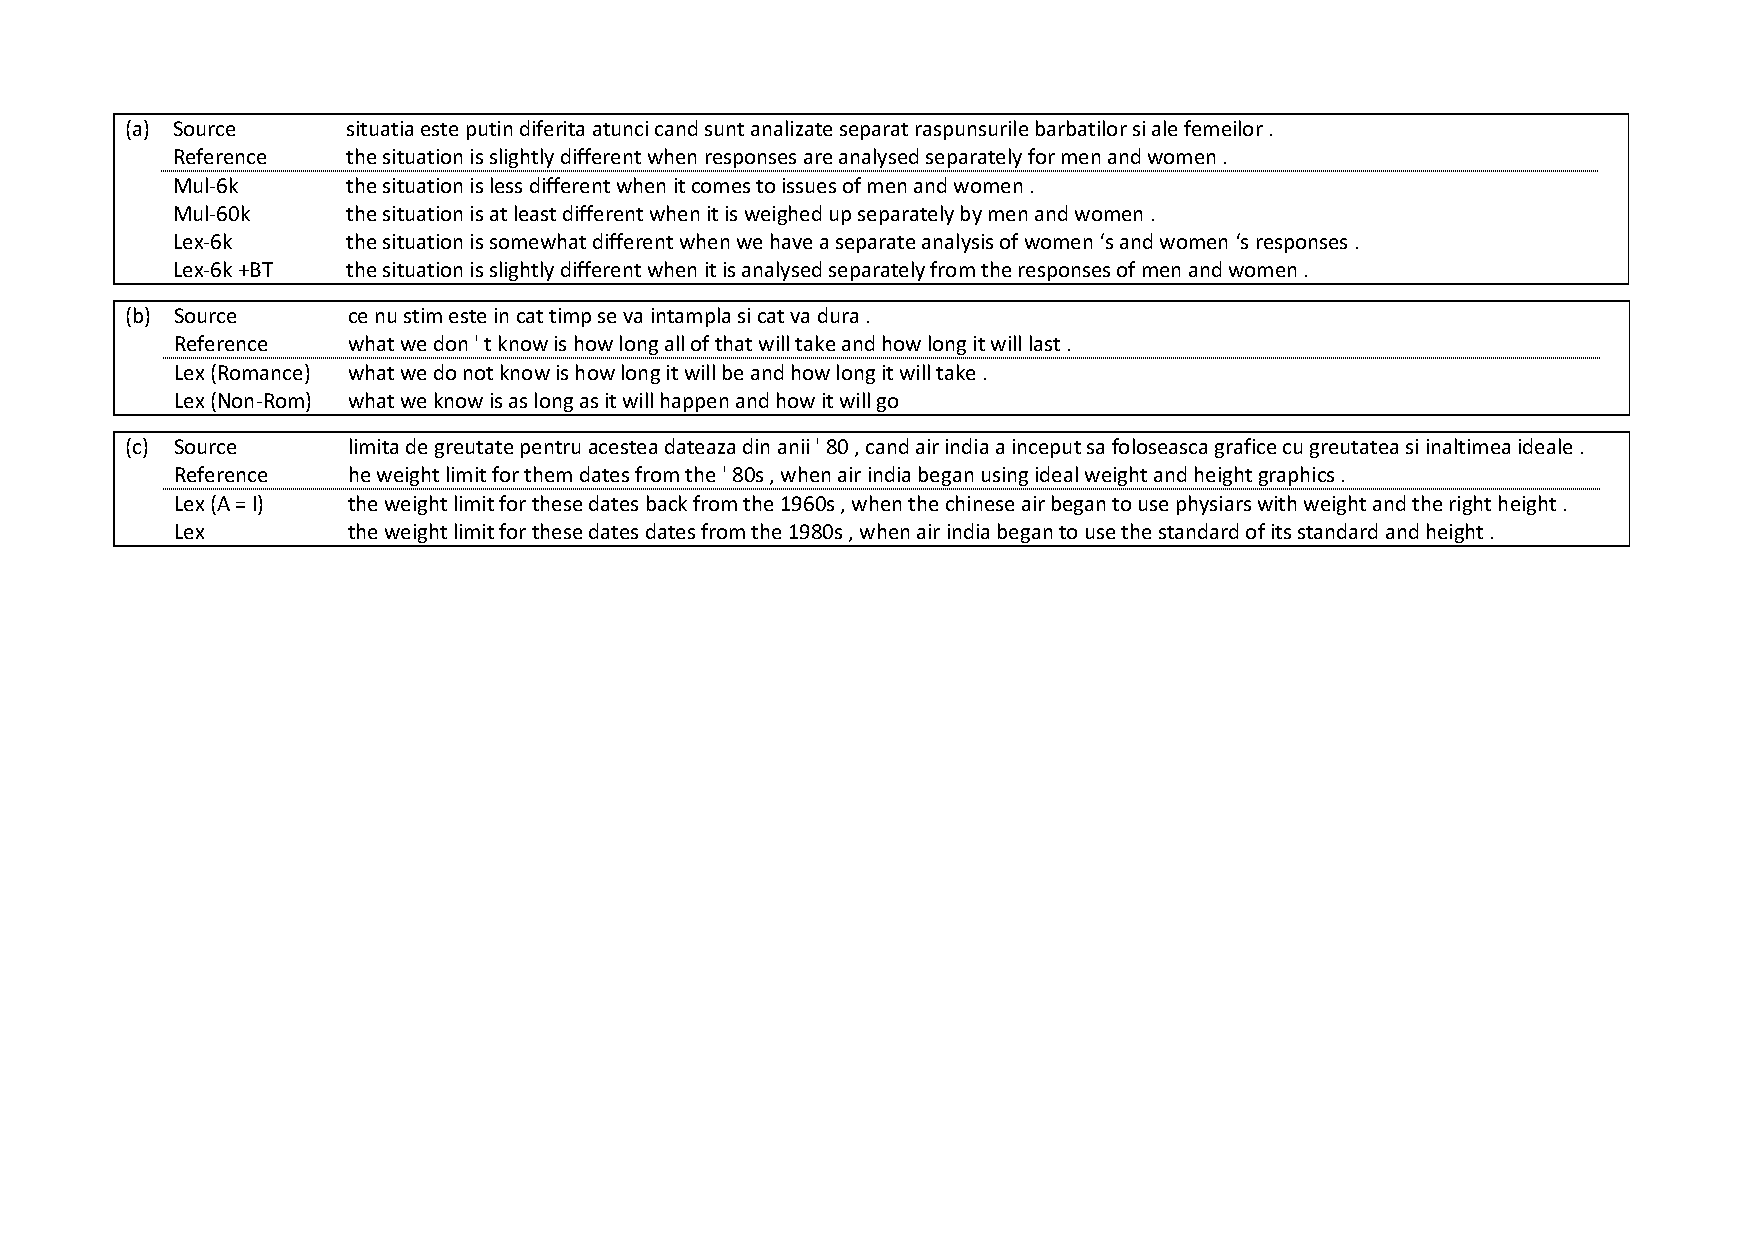
\includegraphics[width=\linewidth]{figs/ulr/examples1}
\caption{\label{cp5.fig.exp}Three sets of examples on Ro-En translation with variant settings. }
\end{sidewaysfigure}
\begin{sidewaysfigure}[hptb]
\centering
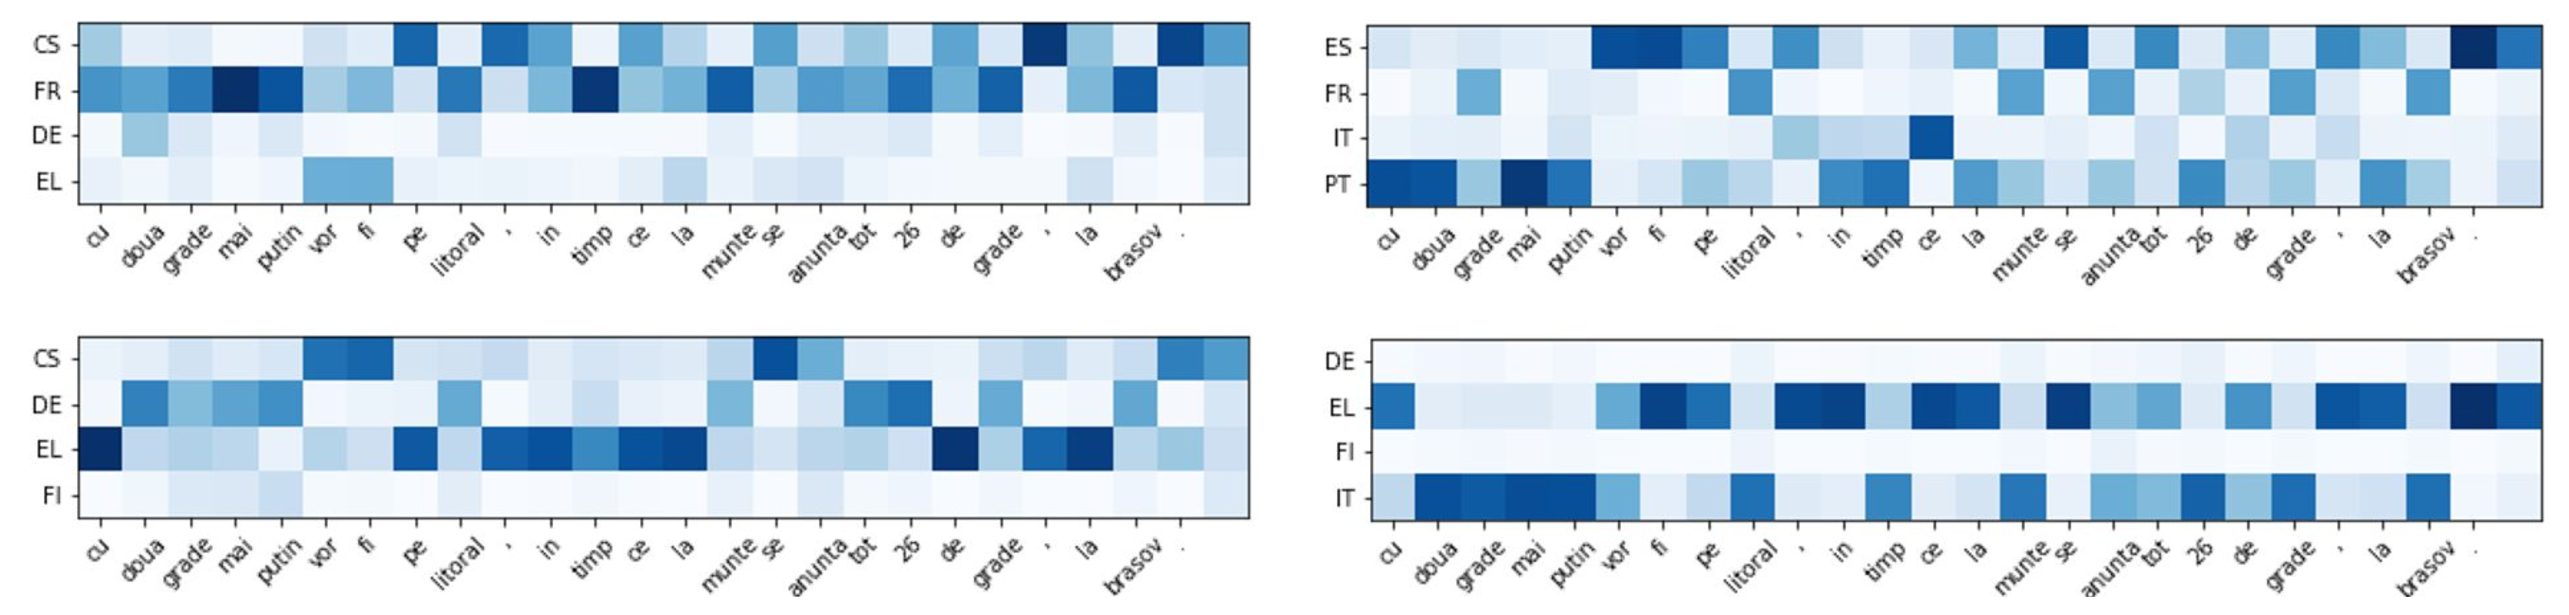
\includegraphics[width=\linewidth]{figs/ulr/vis2}
\caption{\label{cp5.fig.moe} The activation visualization of mixture of language experts module on one randomly selected Ro source sentences trained together with different auxiliary languages. Darker color means higher activation score. }
\end{sidewaysfigure}

\paragraph{Corpus Size}
As shown in Fig.~\ref{cp5.fig.size}, we also evaluated our methods with varied  sizes -- 0k\footnote{For 0k experiments, we used the pre-projection learned from 6k data. It is also possible to use unsupervised learned dictionary.}, 6k, 60k and 600k -- of the Ro-En corpus. The vanilla NMT and the multi-lingual NMT are used as baselines. It is clear in  all cases that the performance gets better when the training corpus is larger. However, the multilingual with ULR works much better with a small amount of training examples. Note that, the usage of ULR universal tokens also enables us to directly work on a ``pure zero" resource translation with a shared multilingual NMT model. 

\paragraph{Unknown Tokens}
One explanation on how ULR help the translation for almost zero resource languages is it greatly cancel out the effects of missing tokens that would cause out-of-vocabularies during testing. As in Fig.~\ref{cp5.fig.missing}, the translation performance heavily drops when it has more ``unknown" which cannot be found in the given 6k training set, especially for the typical multilingual NMT.  Instead, these ``unknown" tokens will naturally have their embeddings based on ULR  projected universal tokens even if we never saw them in the training set. When we apply back-translation over the monolingual data, the performance  further improves which can almost catch up with the model trained with 60k data. %BT helps to handle the sentence-level combination of the ``unknown'' tokens.



% \paragraph{Soft Alignment $q$}
% We also showed the comparison of using different soft-alignment methods in Table~
% \ref{table.q}.
% \begin{table}[htbp]
% 	\centering
%     \begin{tabular}{l|r}
%     Moldel     & BLEU  \\ \hline
%     Multi-NMT  & 14.94 \\ \hline
%     + UnivTok ($R_{\max} = 0$) & 17.08 \\
%     + UnivTok ($R_{\max} = \infty$) & 17.08 \\
%     + UnivTok ($R_{\max} = 300$) & 20.01 \\ \hline
%     + UnivTok ($C_{\min} = 150$) & ~     \\
%     \end{tabular}
%     \caption{Comparison of different confidence coefficient $\alpha$}
% \end{table}

%\begin{table}
%	\centering
%    \begin{tabular}{l|rr}
%    Moldel     & Parallel Only & + BT \\ \hline
%    Multi-NMT  & 14.94         & 17.91       \\
%    + UnivTok  & 20.01          & \textbf{22.35}       \\
%    \end{tabular}
%    \caption{With monolingual data}
%\end{table}


%\begin{figure}
%	\centering
%	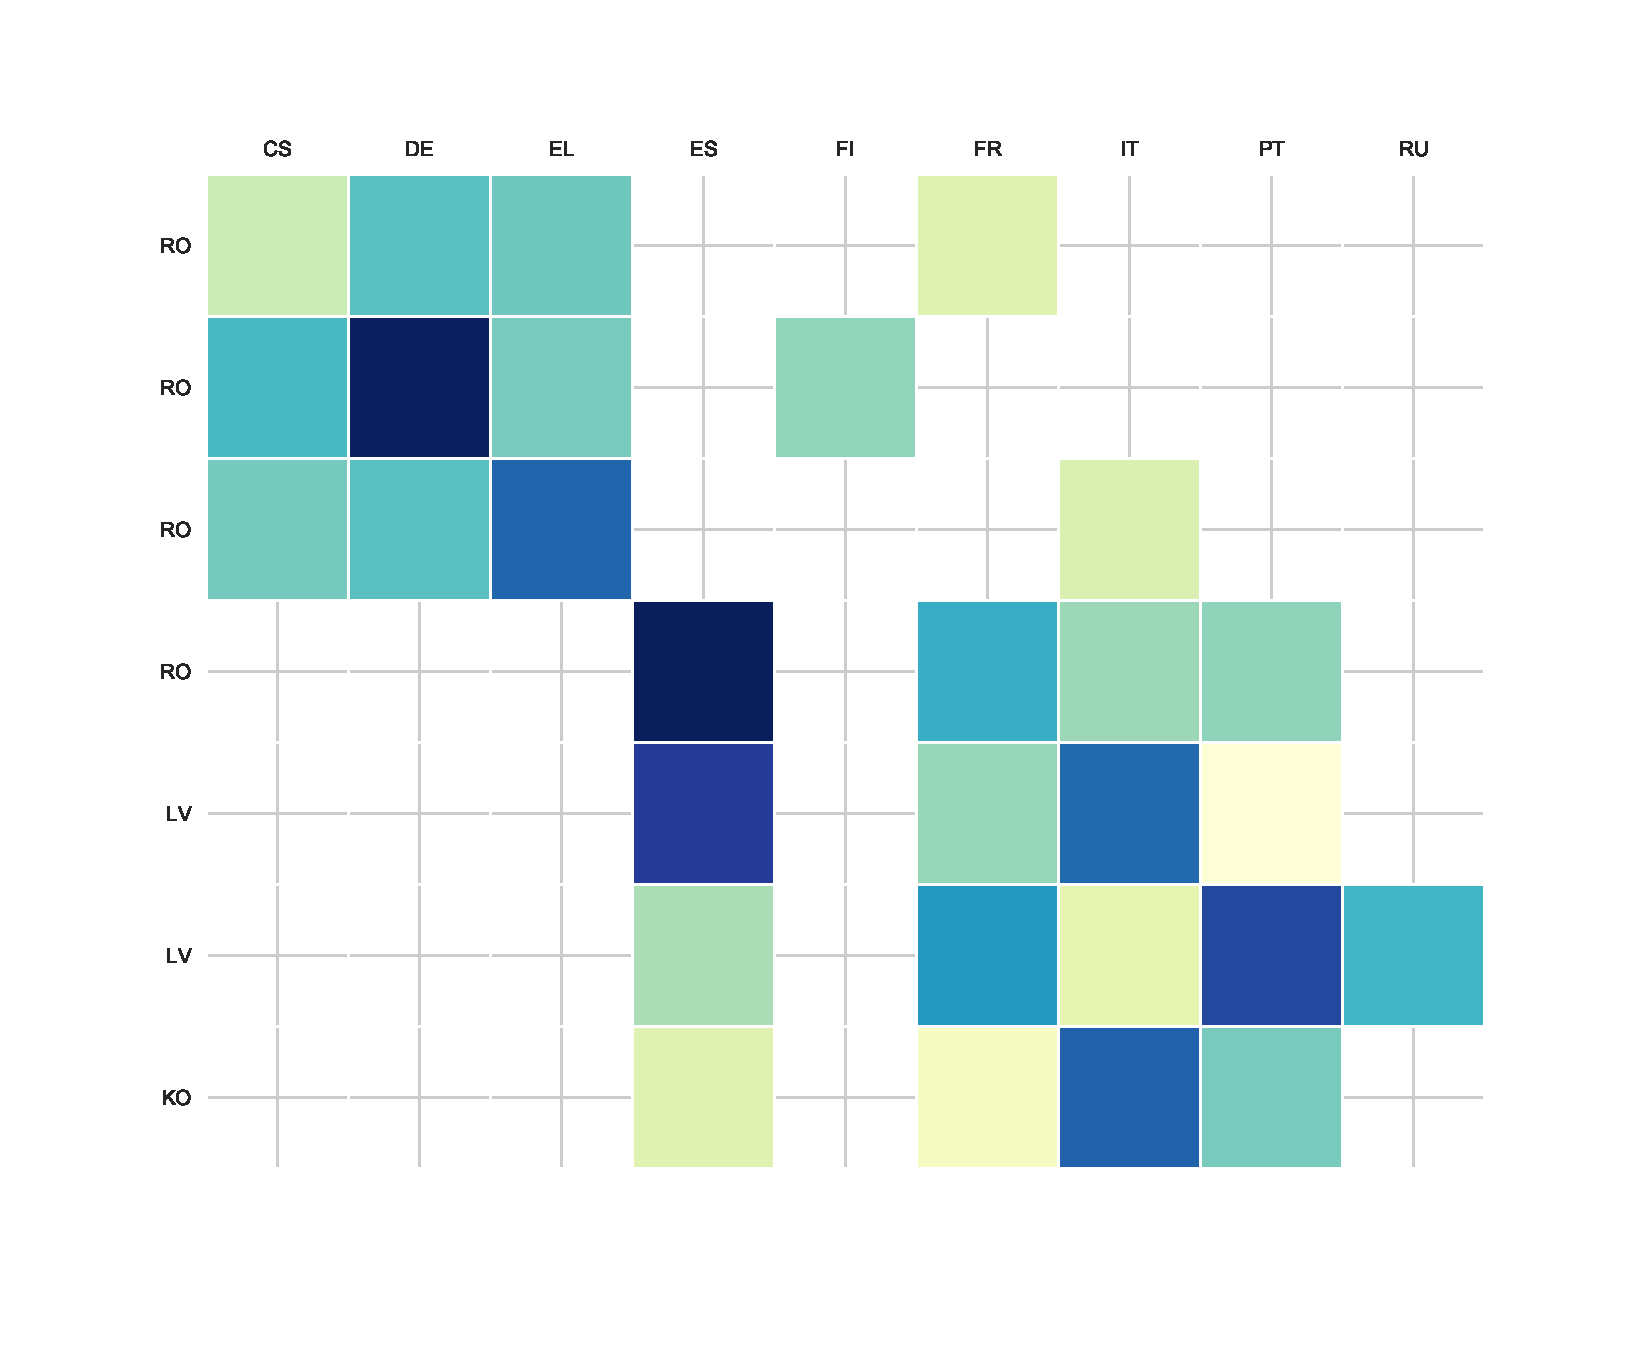
\includegraphics[width=\linewidth]{figs/ulr/multi}\vspace{-20pt}
%	\caption{multilingual experiments}
%\end{figure}

% \subsection{Case Study}
% \paragraph{Examples} As shown in \label{cp5.fig.exp}

\subsection{Qualitative Analysis}
\paragraph{Examples} Figure \ref{cp5.fig.exp} shows some cherry-picked examples for Ro-En. Example (a) shows how the lexical selection get enriched when introducing ULR (Lex-6K) as well as when adding Back Translation (Lex-6K-BT). Example (b) shows the effect of using romance vs non-romance languages as the supporting languages for Ro. Example (c) shows the importance of having a trainable $A$ as have been discussed; without trainable $A$ the model confuses ``india'' and ``china'' as they may have  close representation in the mono-lingual embeddings.

\paragraph{Visualization of MoLE}
Figure \ref{cp5.fig.moe} shows the activations along with the same source sentence with various auxiliary languages. It is clear that MoLE is effectively switching between the  experts when dealing with  zero-resource language words. 
For this particular example of Ro, we can see that the system is utilizing  various auxiliary languages based on their relatedness to the source language. We can approximately rank the relatedness based of the influence of each language. For instance, the influence can be approximately ranked as $\text{Es} \approx \text{Pt} > \text{Fr} \approx \text{It} > \text{Cs} \approx \text{El} > \text{De} > \text{Fi}$, which is interestingly close to the  grammatical relatedness of Ro to these languages. On the other hand, Cs has a strong influence although it does not fall in the same language family with Ro, we think this is due to the geo-graphical influence between the two languages  since  Cs and Ro share similar phrases and expressions. This shows that MoLE learns to utilize resources from similar languages.



% \subsection{Zero Resource Dialect Translation}
% \begin{table}[hptb]
% 	\centering
%     \begin{tabular}{l|rr}
%     Train/ MSA    & Test/ MSA    & Test/ LEV \\ \hline
%     NMT                 & ~  & 17.95        \\
%     + UnivTok (MSA) &~  & 20.37        \\ \hline
%     \end{tabular}
%     \caption{Zero-resource Dialect translation}
% \end{table}
%\subsection{Fine-tuning a Pre-trained Model}
%All  the described experiments above had  the low resource languages  jointly trained  with all the auxiliary high-resource languages, where the training of the large amount of high-resource languages can be seen as a sort of regularization.  It is also common to  train a model on high-resource languages first, and then fine-tune the model on a small resource language similar to transfer learning approaches~\citep{zoph2016transfer}. However, it is not trivial to effectively fine-tune NMT models on extremely low resource data since  the models  easily over-fit due to over-parameterization of the neural networks. 
%
%In this experiment, we have explored the  fine-tuning tasks using our approach. First, we train a Multi-NMT model (with ULR)  on \{Es, Fr, It, Pt\}-En  languages only to create a zero-shot setting for Ro-En translation. Then, we start fine-tuning the model with $6k$ parallel corpora of Ro-En, with and without ULR. As shown in Fig.~\ref{cp5.fig.finetune}, both  models improve a lot over the baseline. 
%%as the multilingual training has provided a good initialization where the extremely low resource language can easily adapt to.
%With the help of ULR, we can  achieve a BLEU score of around $10.7$ (also shown in Fig.~\ref{cp5.fig.size}) for Ro-En translation with ``zero-resource" translation. The BLEU score can  further  improve to almost  $20$ BLEU after 3 epochs of training on $6k$ sentences using ULR. This is almost $6$ BLEU higher than the best score of the baseline. It is worth noting that this fine-tuning is a very efficient  process since it only takes less than 2 minutes to train for 3 epochs over such  tiny amount of data. This is very appealing  for practical applications where  adapting a per-trained system  on-line is a big advantage.  As a future work, we will further investigate a better fine-tuning strategy such as meta-learning~\citep{finn2017model} using ULR.
%
%
%\begin{figure}[hptb]
%	\centering
%	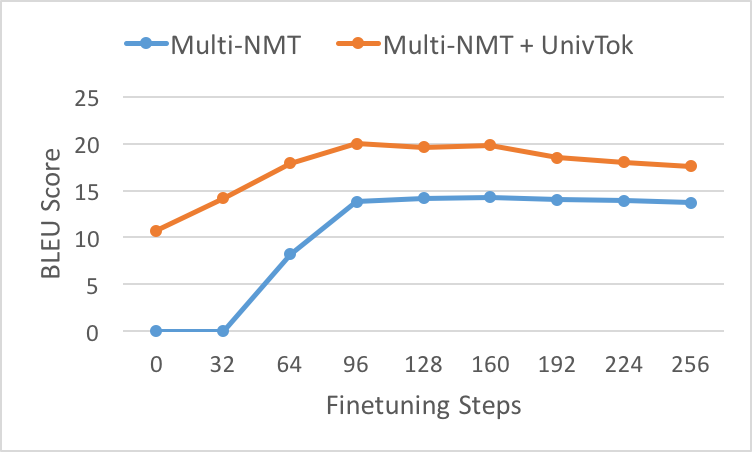
\includegraphics[width=0.80\linewidth]{figs/ulr/finetuning}
%	\caption{\label{cp5.fig.finetune}Performance comparison of Fine-tuning on 6K RO sentences.}
%\end{figure}



\section{Related Work} 
Multi-lingual NMT has been extensively studied in a number of papers such as  \newcite{lee2016fully}, \newcite{johnson2016google}, ~\newcite{zoph2016transfer} and \newcite{firat2016multi}. As we discussed, these approaches have significant limitations with zero-resource cases. \newcite{johnson2016google} is more closely related to our current approach, our work is extending  it  to overcome the  limitations with very low-resource languages and enable sharing of  lexical and sentence representation across multiple languages. 

Two related works are targeting the same problem of  minimally supervised  or totally unsupervised NMT. \newcite{artetxe2017unsupervised} proposed a totally unsupervised approach depending on multi-lingual embedding similar to ours and dual-learning and reconstruction techniques to train the model from mono-lingual data only. \newcite{lample2017unsupervised} also proposed a quite similar approach while utilizing adversarial learning.   

\section{Conclusion and Next Chapter}
 In this chapter, to tackle on the data inefficiency problem for extremely low resource languages, we propose a new  universal machine translation approach that enables sharing translation knowledge from high resource languages.  Our approach is able to achieve 23 BLEU on Romanian-English WMT2016 using a tiny parallel corpus of 6k sentences, compared to the 18 BLEU of strong multi-lingual baseline system. 
 
 However, problems remain in the current solution. One of the main drawbacks of the proposed method is that it relies on joint-training over a huge number of examples of high-resource languages, which is costly and difficult to extend to other new languages. One option is to directly train the model on high resource languages, and fine-tune the trained model on low resource. Also there is no guarantee the pre-trained parameters will be easily fine-tuned by an unknown language. 
 In the next chapter, we will discuss a better way of fine-tuning for extremely low resource languages using meta-learning.
 
 
 

\chapter[Meta Learning for Neural Machine Translation]{Meta Learning for Low Resource Neural Machine Translation}
\label{MetaNMT}

\section{Overview}

Despite the massive success brought by neural machine translation~\citep[NMT,][]{sutskever2014sequence,bahdanau2014neural,vaswani2017attention}, it has been noticed that the vanilla NMT often lags behind conventional machine translation systems, such as statistical phrase-based translation systems~\citep[PBMT,][]{koehn2003statistical}, for low-resource language pairs~\citep[see, e.g.,][]{koehn2017six}. In the past few years, various approaches have been proposed to address this issue. The first attempts at tackling this problem exploited the availability of monolingual corpora~\citep{Gulcehre-Orhan-et-al-2015,sennrich2015improving,zhang2016exploiting}. It was later followed by approaches based on multilingual translation, in which the goal was to exploit knowledge from high-resource language pairs by training a single NMT system on a mix of high-resource and low-resource language pairs~\citep{firat2016multi,firat2016zero,lee2016fully,johnson2016google,ha2016toward}. Its variant, transfer learning, was also proposed by \citet{zoph2016transfer}, in which an NMT system is pretrained on a high-resource language pair before being finetuned on a target low-resource language pair.

In this chapter, we follow up on these latest approaches based on multilingual NMT and propose a meta-learning algorithm for low-resource neural machine translation. We start by arguing that the recently proposed model-agnostic meta-learning algorithm~\citep[MAML,][]{finn2017model} could be applied to low-resource machine translation by viewing language pairs as separate tasks. This view enables us to use MAML to find the initialization of model parameters that facilitate fast adaptation for a new language pair with a minimal amount of training examples (\textsection\ref{cp6.sec.maml-mt}). Furthermore, the vanilla MAML however cannot handle tasks with mismatched input and output. We overcome this limitation by incorporating the universal lexical representation (ULR) introduced in the previous chapter, and adapting it for the meta-learning scenario (\textsection\ref{cp6.sec.ulr}).

We extensively evaluate the effectiveness and generalizing ability of the proposed meta-learning algorithm on low-resource neural machine translation. We utilize 17 languages from Europarl and Russian from WMT as the source tasks and test the meta-learned parameter initialization against five target languages (Ro, Lv, Fi, Tr and Ko), in all cases translating to English. Our experiments using only up to 160k tokens in each of the target task reveal that the proposed meta-learning approach outperforms the multilingual translation approach across all the target language pairs, and the gap grows as the number of training examples decreases.



\section{Background: Meta-Learning}
% \subsection{Low-Resource Neural Machine Translation}
%\paragraph{Neural Machine Translation (NMT)}
%Given a source sentence $X=\{x_1, ..., x_{T'}\}$, a neural machine translation model factors the distribution over possible output sentences $Y=\{y_1, ..., y_T\}$ into a chain of conditional probabilities with a left-to-right causal structure:
%\begin{equation}
%p(Y|X; \theta) = \prod_{t=1}^{T+1} p(y_t| y_{0:t-1}, x_{1:T'}; \theta),
%\end{equation}
%where special tokens $y_0$ ($\langle \mathrm{bos}\rangle$) and $y_{T+1}$ ($\langle \mathrm{eos}\rangle$) are used to represent the beginning and the end of a target sentence.
%These conditional probabilities are parameterized using a neural network. Typically, an encoder-decoder architecture~\citep{sutskever2014sequence,Cho2014a,bahdanau2014neural} with a RNN-based decoder is used. More recently, architectures without any recurrent structures~\citep{gehring2017convolutional,vaswani2017attention} have been proposed and shown to speedup training while achieving state-of-the-art performance.





%\paragraph{Meta Learning}

In the machine learning community, meta-learning, or learning-to-learn, has recently received interests. Meta-learning tries to solve the problem of “fast adaptation on new training data.”  One of the most successful applications of meta-learning has been on few-shot (or one-shot) learning~\citep{lake2015human}, where a neural network is trained to readily learn to classify inputs based on only one or a few training examples. There are two categories of meta-learning:
\begin{enumerate}
    \item learning a meta-policy for updating model parameters~\citep[see, e.g.,][]{andrychowicz2016learning,ha2016hypernetworks,mishra2017meta}
    \item  learning a good parameter initialization for fast adaptation~\citep[see, e.g.,][]{finn2017model,vinyals2016matching,snell2017prototypical}. 
\end{enumerate}
In this paper, we propose to use a meta-learning algorithm for low-resource neural machine translation based on the second category. More specifically, we extend the idea of model-agnostic meta-learning~\citep[MAML,][]{finn2017model} in the multilingual scenario.

% KC: unnecessary here. we will explain the method in detail right below.
% Take the latter as an example, it can be summarized as repeating the following two steps: (1) simulate an episode by sampling a small amounts of training data and “train” a model starting from the meta-model; (2) based on evaluation of the “trained” model, update the meta-model. The ultimate goal of meta-learning and few-shot learning is the same for the case of low resource translation, but there is hardly any work investigating meta-learning for sequence generation tasks such as machine translation. 




\section{Meta-Learning for Extremely Low-Resource Neural Machine Translation}
\label{cp6.sec.maml-mt}

The underlying idea of MAML is to use a set of source tasks $\left\{ \mathcal{T}^1, \ldots, \mathcal{T}^K \right\}$ to find the initialization of parameters $\theta^0$ from which learning a target task $\mathcal{T}^0$ would require only a small number of training examples. In the context of machine translation, this amounts to using many high-resource language pairs to find good initial parameters and training a new translation model on a low-resource language starting from the found initial parameters. This process can be understood as 
\begin{align}
\theta^* = \text{Learn}(\mathcal{T}^0; \text{MetaLearn}(\mathcal{T}^1, \ldots, \mathcal{T}^K)).
\end{align}
That is, we {\it meta-learn} the initialization from auxiliary tasks and continue to {\it learn} the target task. We refer the proposed meta-learning method for NMT to MetaNMT.
See Fig.~\ref{cp6.fig.framework} for the overall illustration. 
\begin{sidewaysfigure}[hptb]
    \centering
    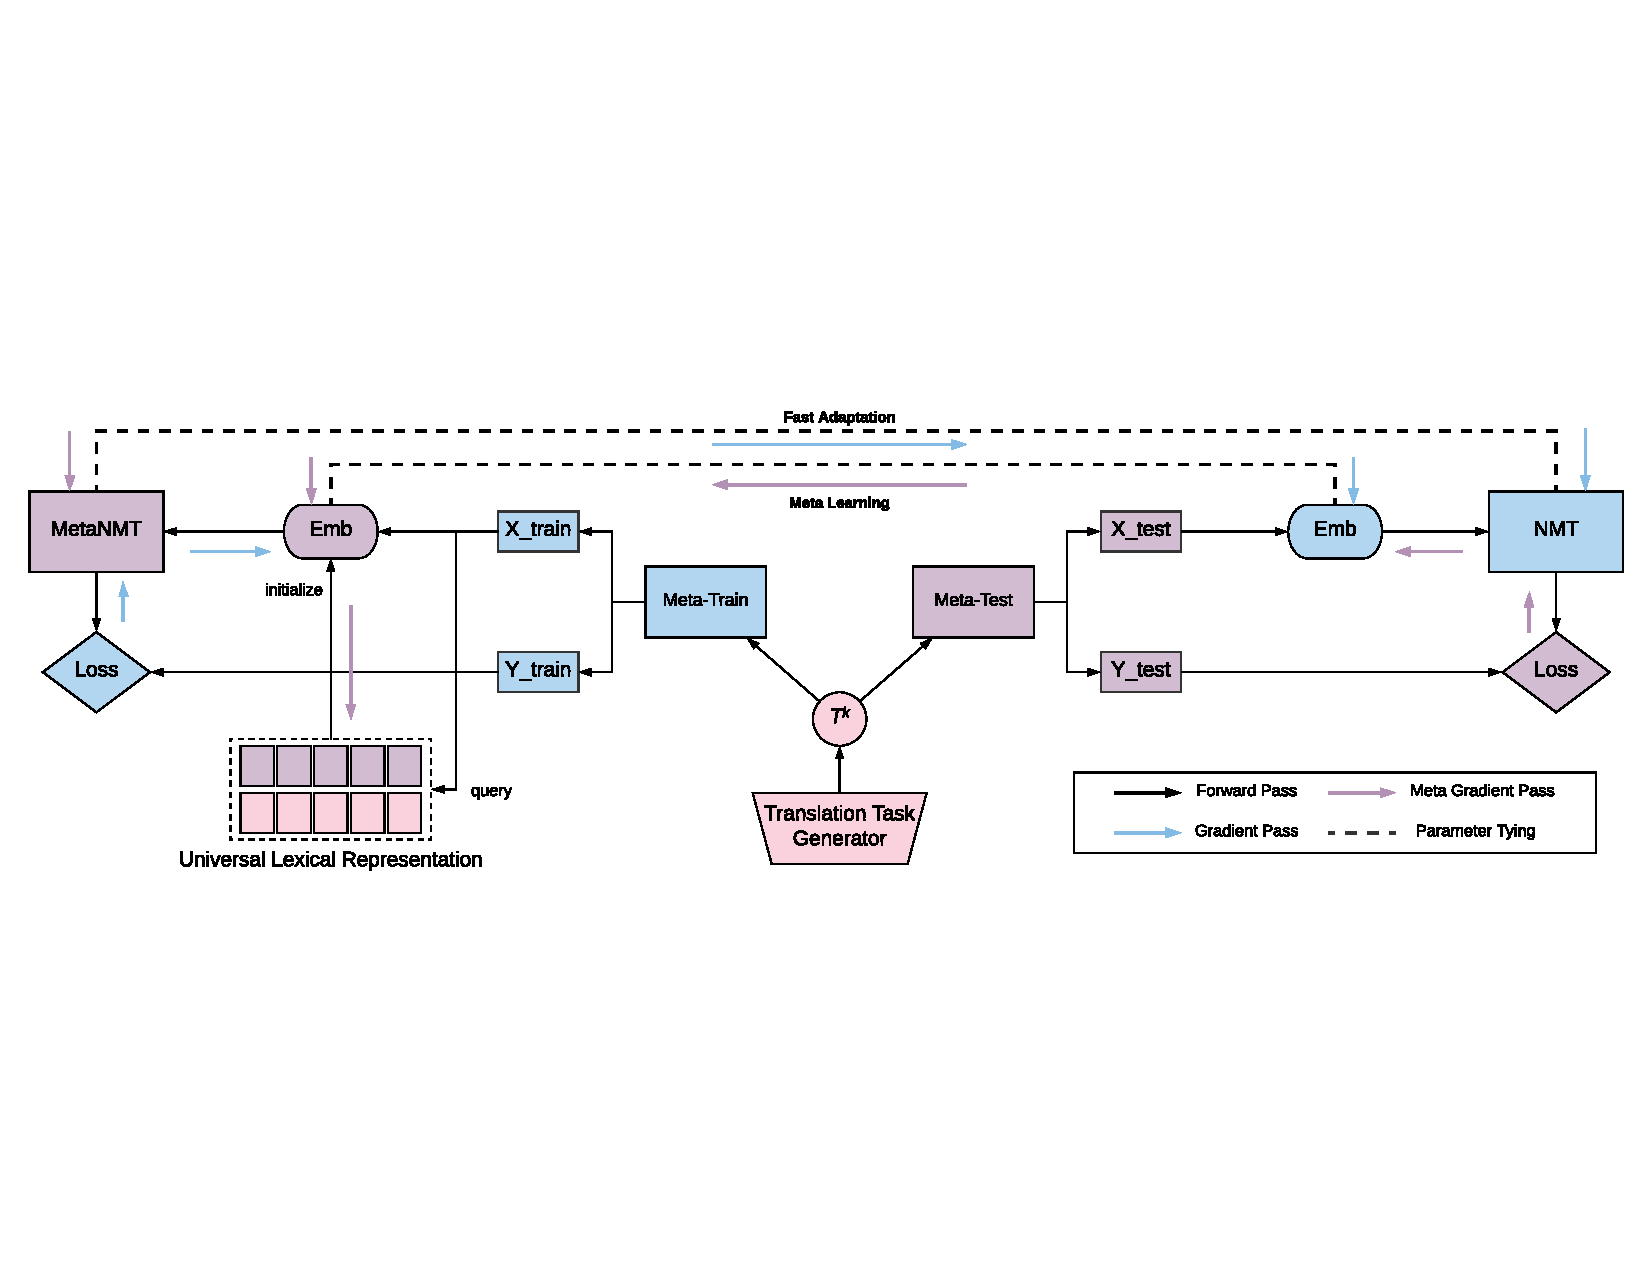
\includegraphics[width=\linewidth]{figs/meta/framework.pdf}
    \caption{The graphical illustration of the training process of the proposed MetaNMT. For each episode, one task (language pair) is sampled for meta-learning. The boxes and arrows in blue are mainly involved in language-specific learning (\textsection\ref{cp6.sec.lsl}), and those in purple in meta-learning (\textsection\ref{cp6.sec.ml}).}
    \label{cp6.fig.framework}
\end{sidewaysfigure}


\subsection{Learn: language-specific learning}
\label{cp6.sec.lsl}
Given any initial parameters $\theta^0$ (which can be either random or meta-learned), 
%We use the meta-learned initial parameters $\theta^0$ to 
the prior distribution of the parameters of a desired NMT model can be defined %a prior distribution over the model parameters 
as an isotropic Guassian:
\begin{align}
    \theta_i \sim \mathcal{N}(\theta^0_i, 1/\beta^2),
\end{align}
where $1/\beta$ is a variance. With this prior distribution, we formulate the language-specific learning process $\text{Learn}(D_\mathcal{T}; \theta^0)$ as maximizing the log-posterior of the model parameters given data $D_{\mathcal{T}}$:
\begin{equation}
	\begin{split}
    &\text{Learn}(D_\mathcal{T}; \theta^0) = 
    \arg\max_{\theta} \mathcal{L}^{D_\mathcal{T}} (\theta)
    \\
    &=\arg\max_{\theta}\!\!\!\!
    \sum_{(X,Y) \in D_{\mathcal{T}}} \!\! \!\!
    \log p(Y | X, \theta)  
    - \beta \| \theta - \theta^0 \|^2,
\end{split}
\end{equation}
where we assume $p(X|\theta)$ to be uniform. 
The first term above corresponds to the maximum likelihood criterion often used for training a usual NMT system. The second term discourages the newly learned model from deviating too much from the initial parameters, alleviating the issue of over-fitting when there is not enough training data. In practice, we solve the problem above by maximizing the first term with gradient-based optimization and early-stopping after only a few update steps. Thus, in the low-resource scenario, finding a good initialization $\theta^0$ strongly correlates the final performance of the resulting model.


\subsection{MetaLearn}
\label{cp6.sec.ml}

We find the initialization $\theta^0$ by repeatedly simulating low-resource translation scenarios using auxiliary, high-resource language pairs. Following \citet{finn2017model} 
%and \citet{al2017continuous}, 
we achieve this goal by defining the meta-objective function as
% \begin{align}
% \label{cp6.eq.meta}
%     \mathcal{L}(\theta) =& 
%     \mathbb{E}_{k,k'} \mathbb{E}_{D_{\mathcal{T}^{k}},D_{\mathcal{T}^{k'}}} \\
%     &\left[
%     \sum_{(X,Y) \in D_{\mathcal{T}^{k'}}} \!\!\!\!\!
%     \log p(Y|X; \text{Learn}(D_{\mathcal{T}^{k}}; \theta))
%     \right], \nonumber
% \end{align}
\begin{align}
\label{cp6.eq.meta}
    \mathcal{L}(\theta) =
    \mathbb{E}_{k} \mathbb{E}_{D_{\mathcal{T}^{k}}, D'_{\mathcal{T}^{k}}} 
    \left[
    \sum_{(X,Y) \in D'_{\mathcal{T}^{k}}} \!\!\!\!\!\!\!
    \log p(Y|X; \text{Learn}(D_{\mathcal{T}^{k}}; \theta))
    \right],
\end{align}
%where $k',k \!\sim\!\mathcal{U}(\left\{1, \ldots, K \right\})$, and $D_{\mathcal{T}}$ follows a uniform distribution over the power set of $\mathcal{T}$.  
where $k \!\sim\!\mathcal{U}(\left\{1, \ldots, K \right\})$ refers to one meta-learning episode, and $D_{\mathcal{T}}$,  $D'_{\mathcal{T}}$ follow the uniform distribution over $\mathcal{T}$'s data.  

We maximize the meta-objective function using stochastic approximation~\citep{robbins1951stochastic} with gradient descent. For each episode, we uniformly sample one source task at random, $\mathcal{T}^{k}$. %and $\mathcal{T}^{k'}$. 
We then sample two subsets of training examples independently from the chosen task, $D_{\mathcal{T}^{k}}$ and $D'_{\mathcal{T}^{k}}$. We use the former to {\it simulate} language-specific learning and the latter to {\it evaluate} its outcome. 
%and $D_{\mathcal{T}^{k'}}$. We use the first one to {\it simulate} learning and the latter to {\it evaluate} its outcome. 
Assuming a single gradient step is taken only the with learning rate $\eta$,
% without loss of generality, 
the simulation is:
\begin{align}
    \theta'_k = \text{Learn}(D_{\mathcal{T}^k}; \theta) =
    \theta - \eta \nabla_{\theta} \mathcal{L}^{D_{\mathcal{T}^k}}(\theta).
\end{align}
Once the simulation of learning is done, we evaluate the updated parameters $\theta'_k$ on $D'_{\mathcal{T}^{k}}$, %$D_{\mathcal{T}^{k'}}$, 
%i.e., $\mathcal{L}^{D'_{\mathcal{T}^{k}}}(\theta'_k)$. 
The gradient computed from this evaluation, which we refer to as {\it meta-gradient}, is used to update the meta model $\theta$. It is possible to aggregate multiple episodes of source tasks before updating $\theta$:
\begin{align}
    \theta \leftarrow \theta - \eta' \sum_k \nabla_\theta \mathcal{L}^{D'_{\mathcal{T}^{k}}}(\theta'_k),
\end{align}
where $\eta'$ is the meta learning rate. 

Unlike a usual learning scenario, the resulting model $\theta^0$ from this meta-learning procedure is not necessarily a good model on its own. It is however a good starting point for training a good model using only a few steps of learning. In the context of machine translation, this procedure can be understood as finding the initialization of a neural machine translation system that could quickly adapt to a new language pair by simulating such a fast adaptation scenario using many high-resource language pairs. 



\paragraph{Meta-Gradient}

% KC: it is not intractable, if we use R-op from Pearlmutter.
% It is intractable to compute the meta-gradient, which requires computing the Hessian matrix, exactly in practice for a usual NMT system which often contains tens of millions of parameters. Instead, 
We use the following approximation property 
\begin{equation}
H(x)v \approx \frac{\nabla(x+\nu v) - \nabla(x)}{\nu}
\end{equation}
to approximate the meta-gradient:\footnote{We omit the subscript $k$ for simplicity.}
\begin{equation}
\begin{split}
	  &\nabla_\theta  \mathcal{L}^{D'}(\theta') = \nabla_{\theta'} \mathcal{L}^{D'}(\theta') 
    \nabla_{\theta}(\theta - \eta \nabla_{\theta} \mathcal{L}^{D}(\theta)) \\
    &= \nabla_{\theta'} \mathcal{L}^{D'}(\theta')
    - \eta \nabla_{\theta'} \mathcal{L}^{D'}(\theta') H_{\theta}(\mathcal{L}^{D}(\theta)) \\
    &\approx 
    \nabla_{\theta'} \mathcal{L}^{D'}(\theta')
    - \frac{\eta}{\nu} \left[
    \nabla_{\theta}\mathcal{L}^D(\theta)\bigg|_{\hat{\theta}}
    - \nabla_{\theta}\mathcal{L}^D(\theta)\bigg|_{\theta} 
    \right],
\end{split}
\end{equation}

% \begin{align*}
%     \nabla_\theta & \mathcal{L}^{D'}(\theta'_k) = \nabla_{\theta'_k} \mathcal{L}^{k'}(\theta'_k) 
%     \nabla_{\theta}(\theta - \eta \nabla_{\theta} \mathcal{L}^{k}(\theta)) \\
%     &= \nabla_{\theta'_k} \mathcal{L}^{k'}(\theta'_k)
%     - \eta \nabla_{\theta'_k} \mathcal{L}^{k'}(\theta'_k) H_{\theta}(\mathcal{L}^{k}(\theta)) \\
%     &\approx 
%     \nabla_{\theta'_k} \mathcal{L}^{k'}(\theta'_k)
%     - \frac{\eta}{\nu} \left(
%     \nabla_{\theta_k}\mathcal{L}^k(\hat{\theta}_k) 
%     - \nabla_{\theta_k}\mathcal{L}^k(\theta_k) 
%     \right),
% \end{align*}
where $\nu$ is a small constant and 
\begin{equation}
	\hat{\theta} = \theta + \nu \nabla_{\theta'}\mathcal{L}^{D'}(\theta').	
\end{equation}

In practice, we find that it is also possible to ignore the second-order term, ending up with the following simplified update rule:
\begin{align}
\label{cp6.eq.meta-grad-first}
    \nabla_\theta \mathcal{L}^{D'}(\theta') \approx
    \nabla_{\theta'} & \mathcal{L}^{D'}(\theta').
\end{align}
%We test both later in the experiments. 




% \alert{KC: TODO}



% \subsection{Fast Adaptation}
% % \paragraph{NMT in an Inference Perspective}
% We focus on finding an optimal neural machine translation system $\theta^*$ which performs well on a new unseen translation pair $\mathcal{T}^0$ with a small number training examples only. One general view is to cast learning of an NMT model $\theta^*$ as maximizing the conditional posterior given the whole training examples:
% \begin{align}
%     \label{eq.learn}
%     %\begin{split}
%     &\text{Learn}(\mathcal{T}^0; \theta^0) \nonumber = \argmax_{\theta} \sum_{X, Y}^{\mathcal{T}^0}\log p(\theta|Y, X)  \\
%     & = \argmax_{\theta} \sum_{X, Y}^{\mathcal{T}^0}\log p(Y | X; \theta) - \beta\cdot \|\theta - \theta^0\|^2 %\nonumber
%     %\end{split}
% \end{align}
% where the first term is the conditional likelihood function, and the second term models the prior of the model. We use $\theta^0$ to denote an initial model. 
% Note that, the first term has a sum over the parallel sentences and dominates the objective as the size of the training examples grows,
% which is the typical MLE objective for training an NMT model. 

% Naive MLE training overfits and does not generalize with low-resource translation. We avoid it by penalizing the model to move too far away from the initial model $\theta^0$. In practise, we implement it implicitly by training the NMT model with the normal MLE objective, while performing early stopping in a small number of gradient steps. 

% \subsection{Meta Learning}
% % \paragraph{Two-step Process}
% Finding an adequate initial model $\theta^0$ highly affects the performance of the resulted final model $\theta^*$. Inspired from previous works~\citep{zoph2016transfer,firat2016multi,lee2016fully,johnson2016google,gu2018universal}, such initialization can be learned over a set of auxiliary multilingual translation pairs $\mathcal{T}^1, ..., \mathcal{T}^K$. As noted by \newcite{finn2017model}, meta-learning is the principal way of learning a good initialization that can quickly adapt to translation of new languages with only a few training examples. It makes much sense for us to recast the learning of Low-Resource NMT as a ``\textit{Meta-Learn $\rightarrow$ Learn}'' process. That is to say,
% \begin{equation}
%     \theta^* = \text{Learn}(\mathcal{T}^0; \text{MetaLearn}(\mathcal{T}^1, ...,\mathcal{T}^K))
% \end{equation}



% \paragraph{Meta Objective}
% Similar to  MAML~\citep{finn2017model}, the initial NMT model $\theta^0$ can be found by repeatedly ``simulating'' a low-resource (Eq.~\ref{eq.learn}) using a set of high-resource translation pairs. Assume that we have $K$ auxiliary pairs $\mathcal{T}^1, ..., \mathcal{T}^K$, our meta-objective for learning a good initialization model $\theta^0$ is:
% \begin{equation}
%     \label{eq.meta}
%     \max_{\theta} \sum_{k=1}^K \sum_{X, Y}^{\mathcal{T}^k} \log p(Y|X; \text{Learn}(\mathcal{T}^k; \theta))
% \end{equation}
% % \begin{equation}
% %     \label{eq.meta}
% %     \begin{split}
% %         &\max_{\theta} \mathbb{E}_k \left[\mathcal{L}^k(\theta')\right] = \\ 
% %         &\mathbb{E}_k \mathbb{E}_{X, Y \sim \mathcal{T}^k} \left[\log p(Y|X; \text{Learn}(\mathcal{T}^k; \theta))\right]
% %     \end{split}
% % \end{equation}
% where we denote $\theta'_k=\text{Learn}(\mathcal{T}^k; \theta)$ as the updated network in the inner-loop which corresponds to simulating low-resource translation sentences by randomly sampling a small fraction of the original dataset and performing only a small number of gradient steps over the sampled data to update the model. The language specific loss $\mathcal{L}^k_{\theta'_k}$ are then computed on a new set of examples from the same language pair with the updated parameters.

% Intuitively, as the same $\theta$ is shared by all the language pairs, the meta-objective implicitly forces the model to learn an initialization which is (1) near language-independent and (2) easy to adapt to new languages. 



% First, sample

% \paragraph{Objective}
% \begin{equation}
%     \max_{\theta} \mathbb{E}_{\mathcal{D}^{\text{train}} \sim W^0} \mathcal{L}^{\text{in}}\left(\mathcal{D}^{\text{train}}; \theta \right),
% \end{equation}

% \begin{equation}
%     \max_{\theta} \mathbb{E}_k \mathbb{E}_{\mathcal{D}^{\text{train}}, \mathcal{D}^{\text{test}} \sim W^k} \mathcal{L}^{\text{out}}\left(\mathcal{D}^{\text{test}}; \theta + \Delta(\mathcal{D}^{\text{train}}; \theta)  \right),
% \end{equation}






\paragraph{Related Work: Multilingual Transfer Learning}

The proposed MetaNMT differs from the existing framework of multilingual translation~\citep{lee2016fully,johnson2016google,gu2018universal} or transfer learning~\citep{zoph2016transfer}. The latter can be thought of as solving the following problem:
\begin{align}
    \max_{\theta} \mathcal{L}^{\text{multi}}(\theta) = \mathbb{E}_k\left[
    \sum_{(X,Y) \in D_k} \log p(Y|X; \theta)
    \right],
\end{align}
where $D_k$ is the training set of the $k$-th task, or language pair. The target low-resource language pair could either be a part of joint training or be trained separately starting from the solution $\theta^0$ found from solving the above problem. 

The major difference between the proposed MetaNMT and these multilingual transfer approaches is that the latter do not consider how learning happens with the target, low-resource language pair. The former explicitly incorporates the learning process within the framework by simulating it repeatedly in Eq.~\eqref{cp6.eq.meta}. As we will see later in the experiments, this results in a substantial gap in the final performance on the low-resource task. 

\paragraph{Illustration}
\begin{figure*}[hptb]
%\sidebysidecaption{0.76\linewidth}{0.23\linewidth}{%
    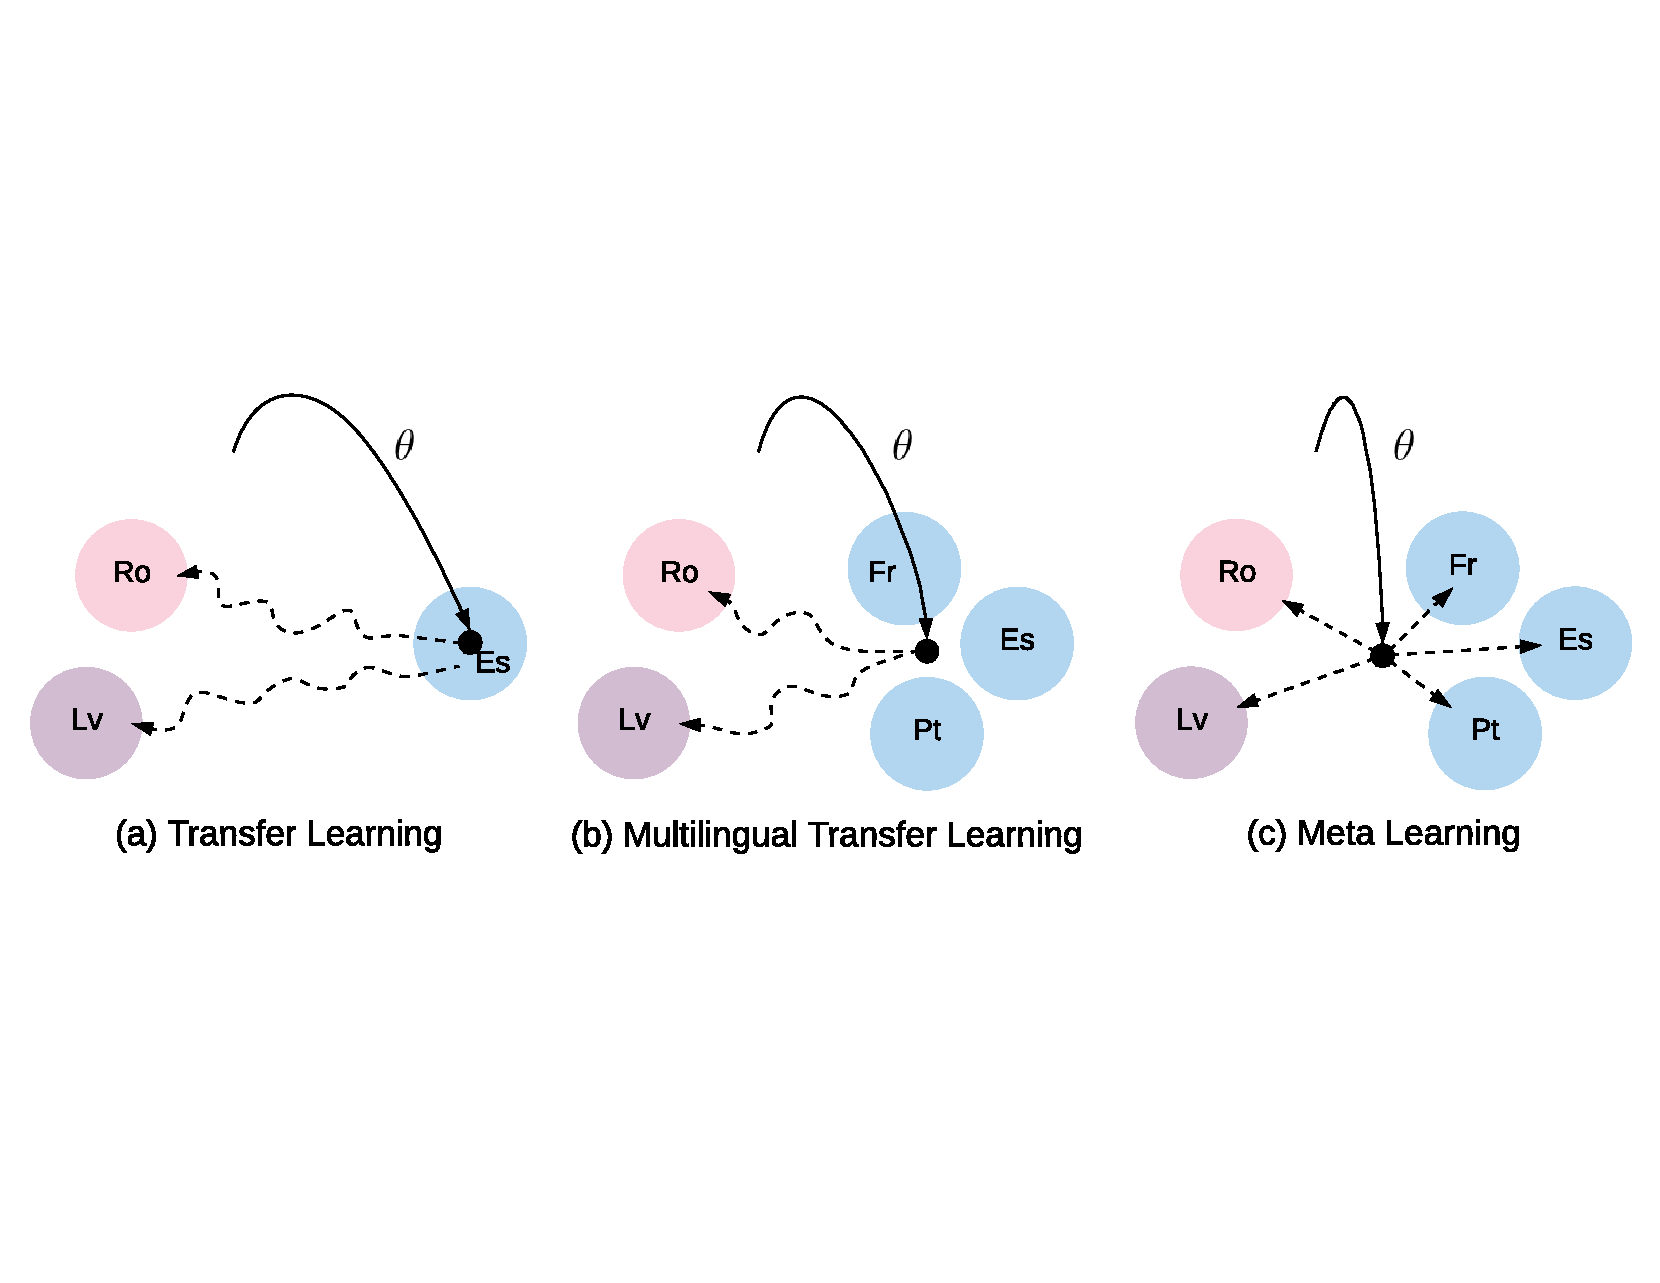
\includegraphics[width=\linewidth]{figs/meta/illust.pdf}%
}
%\vspace{-15pt}
\end{figure*}

In Fig.~\ref{cp6.fig.illustration}, we contrast transfer learning, multilingual learning and meta-learning using three source language pairs (Fr-En, Es-En and Pt-En) and two target pairs (Ro-En and Lv-En). Transfer learning trains an NMT system specifically for a source language pair (Es-En) and finetunes the system for each target language pair (Ro-En, Lv-En). Multilingual learning often trains a single NMT system that can handle many different language pairs (Fr-En, Pt-En, Es-En), which may or may not include the target pairs (Ro-En, Lv-En). If not, it finetunes the system for each target pair, similarly to transfer learning. Both of these however aim at directly solving the source tasks. On the other hand, meta-learning trains the NMT system to be {\it useful for fine-tuning} on various tasks including the source and target tasks. This is done by repeatedly simulating the learning process on low-resource languages using many high-resource language pairs (Fr-En, Pt-En, Es-En). 



% which has been proved very successful on low-resource neural machine translation. 

% The major difference is that, for multi-ligual transfer learning, the objective is to jointly optimize the likelihood across multiple languages with most of the parameters shared. The target low resource language can be either jointly training with other languages, or be fine-tuned after trained on high resource languages. Similar to Eq.~\ref{eq.meta} we have
% \begin{equation}
%     \label{eq.multi}
%     \max_{\theta} \sum_{k=1}^K \sum_{X, Y}^{\mathcal{T}^k} \log p(Y|X; \theta)
% \end{equation}
% where we do not have inner-loop updates. 

% TODO: Intert a discussion about Figure.2

\subsection{Unified Lexical Representation}% for MetaNMT}
\label{cp6.sec.ulr}

%\todo{KC: shorten this section. It's really difficult to shorten it.}

\paragraph{I/O mismatch across language pairs}
One major challenge that limits applying meta-learning for low resource machine translation is that
the approach outlined above assumes the input and output spaces are shared across all the source and target tasks. This, however, does not apply to machine translation in general due to the vocabulary mismatch across different languages. In multilingual translation, this issue has been tackled by using a vocabulary of sub-words~\citep{sennrich2015improving} or characters~\citep{lee2016fully} shared across multiple languages. This surface-level sharing is however limited, as it cannot be applied to languages exhibiting distinct orthography (e.g., Indo-Euroepan languages vs. Korean.) 

% One major challenge that limits applying MAML for NMT is that this learning algorithm implicitly assumes similar a I/O space at training and testing so that it can be adapted quickly with few examples. 
% %It is natural for tasks such as few-shot image classification where raw pixels are used as inputs. 
% However for NMT, each token from one language is firstly associated with an embedding vector $\epsilon[x]$ based on an unique token index $x$ before read by the following layers. $\epsilon$ is the embedding matrix which is trained jointly with $\theta$\footnote{For simplicity, we denote $\epsilon$ as the embedding, while $\theta$ as the rest of parameters of an NMT model.} from random initialization and typically differs across languages. 

% Therefore, although different languages share intrinsic similarities at both syntactic and semantic levels, the conventional MAML cannot learn good initialization for the embedding for fast adaptation.
% %the target language pairs might not even share the vocabularies with all other languages during training. 
% \alert{KC: the following is not an issue with the I/O space mismatch, but the issue of sparsity.}
% Furthermore, for translating very low resource languages (e.g., hundreds of training examples), a large proportion of tokens may never appear during adaptation, which is impossible to get meaningful translation for them.

\paragraph{Universal Lexical Representation (ULR)} 

We tackle this issue by dynamically building a vocabulary specific to each language using a key-value memory network~\citep{miller2016key,gulcehre2018dynamic}, which was introduced in detail in Chapter~\ref{ulr}, in \S\ref{cp5.sec.unilex} as the universal lexical representation (ULR) where we formulate the universal embedding for each word $x$ as a weighted sum of the embeddings $\epsilon_U$ of a set of universal tokens $u_1, ..., u_M$. Here we use the resulted universal embedding matrix for each word (as computed in Eq.~\eqref{cp5.eq.universal_embed}) as the initialized embedding $\epsilon^0[x]$ for each word of each input language.


%done successfully for low-resource machine translation recently by \citet{gu2018universal}. We start with multilingual word embedding matrices $\epsilon^k_{\text{query}} \in \mathbb{R}^{|V_k| \times d}$ pretrained on large monolingual corpora, where $V_k$ is the vocabulary of the $k$-th language. These embedding vectors can be obtained with small dictionaries of seed word pairs~\citep{artetxe2017learning,smith2017offline} or in a fully unsupervised manner~\citep{zhang2017earth,alexis2018word}. We take one of these languages $k'$ to build universal lexical representation consisting of a universal embedding matrix $\epsilon_u \in \mathbb{R}^{M \times d}$ and a corresponding
%% KC: $k$ is overloaded with too many semantics
%key matrix $\epsilon_{\text{key}} \in \mathbb{R}^{M \times d}$, where $M < |V_k'|$. Both $\epsilon^k_{\text{query}}$ and $\epsilon_{\text{key}}$ are fixed during meta-learning. We then compute the language-specific embedding of token $x$ from the language $k$ as the convex sum of the universal embedding vectors by
%\[
%\epsilon^0[x] = \sum_{i=1}^M \alpha_i \epsilon_u[i],
%\]
%where 
%$\alpha_i \propto \exp\left\{ -\tfrac{1}{\tau} \epsilon_{\text{key}}[i]^\top A \epsilon^k_{\text{query}} [x] \right\}$ and $\tau$ is set to $0.05$. This approach allows us to handle languages with different vocabularies using a fixed number of shared parameters ($\epsilon_u$, $\epsilon_{\text{key}}$ and $A$.) 

\paragraph{Learning of ULR}

It is not desirable to update the universal embedding matrix $\epsilon_U$ when fine-tuning on a small corpus which contains a limited set of unique tokens in the target language, as it could adversely influence the other tokens' embedding vectors. We thus estimate the change to each embedding vector induced by language-specific learning by a separate parameter $\Delta \epsilon^k[x]$:
\begin{equation}
	\epsilon^k[x] = \epsilon^0[x] + \Delta \epsilon^k[x].
\end{equation}
During language-specific learning, the ULR $\epsilon^0[x]$ is held constant, while only $\Delta \epsilon^k[x]$ is updated, starting from an all-zero vector. On the other hand, we hold $\Delta \epsilon^k[x]$'s constant while updating $\epsilon_U$ and $A$ during the meta-learning stage. 


% \alert{KC: TODO}

% Tackling on above challenges, it is essential to have a unified I/O space for MetaNMT. 
% For instance, considering the surface similarities (e.g. spelling, morphology, etc.), we can use a subword-based or character-based~\cite{lee2016fully} model to enforce all the languages share the same vocabularies. However, such surface-level sharing has limitations to apply to distinct languages (e.g. Indo-European languages and Korean). In practise, we also found that sharing sub-words fails when given extremely limited training data even for similar languages.

% Instead, we utilize a simple but effective method based on projected monolingual embedding which was recently proposed in \newcite{gu2018universal}. More precisely, we define a space for $M$ universal lexical tokens with the trainable embedding matrix $\epsilon_u\in\mathbb{R}^{M\times d}$. Thus, we can represent each input token $x$ from any language by querying with a distance measure $d(u_i,x)$:
% \begin{equation}
%  \label{eq.source word}
% \epsilon^0[x]=\sum_{i=1}^M\epsilon_u[u_i]\cdot \text{softmax}\left({-d(u_i,x)}/{\tau}\right),
% \end{equation}
% % where $q(u_i|x)$ is a conditional distribution in universal token space. $q(u_i|x)$ is computed by the distance metric:
% % \begin{equation}
% %  \label{eq.q distance}
% % q(u_i|x)=\frac{e^{\frac{d(u_i,x)}{\tau}}}{\sum_i e^{\frac{d(u_i,x)}{\tau}}},
% % \end{equation}
% where $\tau$ is the temperature. Following \newcite{gu2018universal}, one way to compute the distance is:
% %$d(u_i,x)$ measures the similarity between source word $x$ and universal token $u_i$ and it can be obtained by:
% \begin{equation}
%  \label{eq.d distance}
% d(u_i, x)=-\epsilon_k(u_i)\cdot A\cdot\epsilon_q(x)^\top,
% \end{equation}
% where $\epsilon_k$ are the \textit{key} vectors for universal tokens, and $\epsilon_q$ are the \textit{query} vectors for any specific input language. Both of the vectors are fixed can be easily obtained by learning embeddings from large monolingual corpora and then being projected to the same space based on a small dictionary\cite{smith2017offline} or in unsupervised~\cite{zhang2017earth,alexis2018word}. The transformation matrix $A$ initialized with identity matrix is learned in the training process.

% \paragraph{ULR as Initialized Word Embedding} 

% One major difference with \newcite{gu2018universal} is that in their work, the resulted universal vector (Eq.~\ref{eq.source word}) is jointly used with an individual embedding trained independently for each token. In contrast for meta learning, we assume each token only has one embedding $\epsilon[x]$ that is specially initialized by $\epsilon^0[x]$. It is equivalent to treat $\epsilon^0[x]$ as constant and learn an difference $\Delta\epsilon[x]$ in the inner-loop, while passing gradients from the updated vector $\Delta\epsilon[x] + \epsilon^0[x]$ to $\epsilon_u$ and $A$ in the outer-loop from Eq.~\ref{eq.source word} and \ref{eq.d distance}.


% \subsection{Unified I/O Space for MetaNMT}

% %\todo{KC: shorten this section. It's really difficult to shorten it.}

% \paragraph{Challenges}
% One major challenge that limits applying MAML for NMT is that the learning algorithm learns the network initialization for all the tasks, implicitly assuming similar a I/O space at training and testing so that it can be adapted quickly with few examples. %It is natural for tasks such as few-shot image classification where raw pixels are used as inputs. 
% However for NMT, each token from one language is firstly associated with an embedding vector $\epsilon[x]$ based on an unique token index $x$ before read by the following layers. $\epsilon$ is the embedding matrix which is trained jointly with $\theta$\footnote{For simplicity, we denote $\epsilon$ as the embedding, while $\theta$ as the rest of parameters of an NMT model.} from random initialization and typically differs across languages. 

% Therefore, although different languages share intrinsic similarities at both syntactic and semantic levels, the conventional MAML cannot learn good initialization for the embedding for fast adaptation.
% %the target language pairs might not even share the vocabularies with all other languages during training. 
% Furthermore, for translating very low resource languages (e.g., hundreds of training examples), a large proportion of tokens may never appear during adaptation, which is impossible to get meaningful translation for them.

% \paragraph{Universal Lexical Representation} Tackling on above challenges, it is essential to have a unified I/O space for MetaNMT. 
% For instance, considering the surface similarities (e.g. spelling, morphology, etc.), we can use a subword-based or character-based~\cite{lee2016fully} model to enforce all the languages share the same vocabularies. However, such surface-level sharing has limitations to apply to distinct languages (e.g. Indo-European languages and Korean). In practise, we also found that sharing sub-words fails when given extremely limited training data even for similar languages.

% Instead, we utilize a simple but effective method based on projected monolingual embedding which was recently proposed in \newcite{gu2018universal}. More precisely, we define a space for $M$ universal lexical tokens with the trainable embedding matrix $\epsilon_u\in\mathbb{R}^{M\times d}$. Thus, we can represent each input token $x$ from any language by querying with a distance measure $d(u_i,x)$:
% \begin{equation}
%  \label{eq.source word}
% \epsilon^0[x]=\sum_{i=1}^M\epsilon_u[u_i]\cdot \text{softmax}\left({-d(u_i,x)}/{\tau}\right),
% \end{equation}
% % where $q(u_i|x)$ is a conditional distribution in universal token space. $q(u_i|x)$ is computed by the distance metric:
% % \begin{equation}
% %  \label{eq.q distance}
% % q(u_i|x)=\frac{e^{\frac{d(u_i,x)}{\tau}}}{\sum_i e^{\frac{d(u_i,x)}{\tau}}},
% % \end{equation}
% where $\tau$ is the temperature. Following \newcite{gu2018universal}, one way to compute the distance is:
% %$d(u_i,x)$ measures the similarity between source word $x$ and universal token $u_i$ and it can be obtained by:
% \begin{equation}
%  \label{eq.d distance}
% d(u_i, x)=-\epsilon_k(u_i)\cdot A\cdot\epsilon_q(x)^\top,
% \end{equation}
% where $\epsilon_k$ are the \textit{key} vectors for universal tokens, and $\epsilon_q$ are the \textit{query} vectors for any specific input language. Both of the vectors are fixed can be easily obtained by learning embeddings from large monolingual corpora and then being projected to the same space based on a small dictionary\cite{smith2017offline} or in unsupervised~\cite{zhang2017earth,alexis2018word}. The transformation matrix $A$ initialized with identity matrix is learned in the training process.

% \paragraph{ULR as Initialized Word Embedding} One major difference with \newcite{gu2018universal} is that in their work, the resulted universal vector (Eq.~\ref{eq.source word}) is jointly used with an individual embedding trained independently for each token. In contrast for meta learning, we assume each token only has one embedding $\epsilon[x]$ that is specially initialized by $\epsilon^0[x]$. It is equivalent to treat $\epsilon^0[x]$ as constant and learn an difference $\Delta\epsilon[x]$ in the inner-loop, while passing gradients from the updated vector $\Delta\epsilon[x] + \epsilon^0[x]$ to $\epsilon_u$ and $A$ in the outer-loop from Eq.~\ref{eq.source word} and \ref{eq.d distance}.
% \subsection{Meta-Learning for Semi-Supervised Low Resource Translation}
% Not sure if it will work or not yet


% The overall algorithm can be seen as follows:
% \begin{algorithm}[H]
% \caption{Learning for Meta-NMT (placeholder as long as possible)}
% \label{algo1}
% \begin{algorithmic}[1]
% \small
% \Require{MT model ${\theta}$.}
% \State Initialize 
% \While{stopping criterion is not met}
% \For{$k=1...K$}  
% \State Let $Y'_k = \{y'_1, ..., y'_{T'}\}, X'_k = \{x'_1, ..., x'_{T'_s}\}$
% \For{$\tau=1...T'$}
% \State Generate key $c'_\tau = f_{\text{att}}(y'_{<\tau}, X'_k)$
% \EndFor 
% \EndFor
% \State Update $\phi \leftarrow \phi  +\gamma\frac{\partial}{\partial \phi} \sum_{t=1}^T\log p(y_t|\cdot)$
% \EndWhile
% \end{algorithmic}
% \end{algorithm}


\section{Experiments}
\label{cp6.sec.exps}

%We extensively study the effectiveness of the proposed MetaNMT for fast parameter adaptation of NMT given limited training examples. We evaluated the algorithm on four simulated low resource language pairs with variant auxiliary languages used for meta-training. Both random initialization and multilingual training are used as baselines.

\subsection{Dataset}

%\paragraph{Dataset} We empirically evaluate the proposed \textsc{ZR-NMT} on $4$ languages -- Romanian (Ro) / Latvian (LV) / Korean (KO) / Levantine Arabic (LEV)\footnote{A spoken dialect of standard Arabic.} -- translating to English (En) in near zero-resource settings. To achieve this, single or multiple auxiliary languages from Czech (Cs), German (De), Greek (El), Spanish (Es), Finnish (Fi), French (Fr),  Italian (It), Portuguese (Pt), Russian (Ru) and Modern Standard Arabic (MSA) are jointly trained to translate to English.

\paragraph{Target Tasks}
We show the effectiveness of the proposed meta-learning method for low resource NMT with extremely limited training examples on five diverse target languages: Romanian (Ro) from WMT'16,\footnote{
\url{http://www.statmt.org/wmt16/translation-task.html}
}
Latvian (Lv), Finnish (Fi), Turkish (Tr) from WMT'17,\footnote{
\url{http://www.statmt.org/wmt17/translation-task.html}
}
and Korean (Ko) from Korean Parallel Dataset.\footnote{
\url{https://sites.google.com/site/koreanparalleldata/}
}
We use the officially provided train, dev and test splits for all these languages. %\alert{how do we split Ko?}
The statistics of these languages are presented in Table~\ref{cp6.table.full-dataset}. We simulate the low-resource translation scenarios by randomly sub-sampling the training set with different sizes.

\begin{table}[hptb]
\centering
%\resizebox{\textwidth}{!}{
\begin{tabular}{rcc|rr}
\toprule
%  &\multicolumn{2}{c}{Bleu score}&\multicolumn{2}{c}{Bleu score}\\
& \# of sents. & \# of En tokens & Dev & Test\\
\midrule
Ro-En&$0.61$ M &$16.66$ M&$-$&$31.76$  \\
Lv-En&$4.46$ M &$67.24$ M&$20.24$&$15.15$\\
Fi-En&$2.63$ M &$64.50$ M&$17.38$&$20.20$  \\
Tr-En&$0.21$ M & \ \ $5.58$ M &$15.45$&$13.74$ \\
Ko-En&$0.09$ M & \ \ $2.33$ M &$6.88$&$5.97$ \\
\bottomrule
\end{tabular}
%}
\caption{Statistics of full datasets of the target language pairs. BLEU scores on the dev and test sets are reported from a supervised Transformer model with the same architecture.}
\label{cp6.table.full-dataset}
\end{table}



\paragraph{Source Tasks}

We use the following languages from Europarl\footnote{
\url{http://www.statmt.org/europarl/}
}:
Bulgarian (Bg),
Czech (Cs), 
Danish (Da),
German (De),
Greek  (El),
Spanish (Es),
Estonian  (Et),
French (Fr),
Hungarian   (Hu),
Italian (It),
Lithuanian  (Lt),
Dutch   (Nl),
Polish  (Pl),
Portuguese  (Pt),
Slovak  (Sk),
Slovene (Sl) and
Swedish (Sv), in addition to Russian (Ru)\footnote{
A subsample of approximately 2M pairs from WMT'17.
} to learn the intilization for fine-tuning. In our experiments, different combinations of source tasks are explored to see the effects from the source tasks.

% We employ $18$ languages as source tasks during meta-train, which includes all languages from Europarl\footnote{http://www.statmt.org/europarl/} except for those used as target tasks, i.e., 
% Bulgarian (Bg),
% Czech (Cs), 
% Danish (Da),
% German (De),
% Greek  (El),
% Spanish (Es),
% Estonian  (Et),
% French (Fr),
% Hungarian   (Hu),
% Italian (It),
% Lithuanian  (Lt),
% Dutch   (Nl),
% Polish  (Pl),
% Portuguese  (Pt),
% Slovak  (Sk),
% Slovene (Sl),
% Swedish (Sv). In addition, a subset ($\sim 2$ M sentence pairs) of Russian (Ru) from WMT'17 is also incorporated. In our experiments, different combinations of source tasks are explored to see the effects take from the source tasks.



\paragraph{Validation}

We pick either Ro-En or Lv-En as a validation set for meta-learning and test the generalization capability on the remaining target tasks. This allows us to study the strict form of meta-learning, in which target tasks are unknown during both training and model selection.




% 

% Ro and Lv are selected to be the meta-validation sets which are utilized to track the progress of the meta-model. Under this setting, we can carefully investigate the generalization capability of the proposed meta-learning approach. 

% By default, we only consider $\rightarrow\!\text{En}$ tasks. 
% We consider $4$ diverse languages as the main target tasks, including Romanian (Ro) from WMT'16\footnote{http://www.statmt.org/wmt16/translation-task.html}, Latvian (Lv), Finnish (Fi) and Turkish (Tr) from WMT'17\footnote{http://www.statmt.org/wmt17/translation-task.html} with official train, dev and test datasets. For an optional comparison with very distant languages, we also investigate using Korean (Ko)\footnote{https://sites.google.com/site/koreanparalleldata/} as the exceptional target language. The detailed statistics of the target tasks are shown in Table.~/ref{table:full dataset}, some of which are low resource-enough already. 
% In our experiments, random sampling are further performed to simulate extremely low resource settings from which we test the effectiveness of the proposed method. 


\paragraph{Preprocessing and ULR Initialization}

As described in \textsection\ref{cp6.sec.ulr}, we initialize the query embedding vectors $\epsilon_{K}^k$ of all the languages. For each language, we use the monolingual corpora built from Wikipedia\footnote{
We use the most recent Wikipedia dump (2018.5) from \url{https://dumps.wikimedia.org/backup-index.html}. 
}
and the parallel corpus. The concatenated corpus is first tokenized and segmented using byte-pair encoding~\citep[BPE,][]{sennrich2016edinburgh}, resulting in $40,000$ subwords for each language. We then estimate word vectors using fastText~\citep{bojanowski2016enriching}. Different from the method proposed in Chapter~\ref{ulr} where we used a short-list of seed words to align the embeddings, we align the pre-trained word embeddings across all the languages in an unsupervised way using MUSE~\citep{alexis2018word} to get multilingual word vectors. We use the multilingual word vectors of the 20,000 most frequent words in English to form the universal embedding matrix $\epsilon_U$. 
% Following \citet{gu2018universal}, tokens of all other languages are attached with special language tags.



% We empirically evaluate the proposed Universal NMT system on $3$ languages -- Romanian (Ro) / Latvian (Lv) / Korean (Ko)  -- translating to English (En) in near zero-resource settings. To achieve this, single or multiple auxiliary languages from Czech (Cs), German (De), Greek (El), Spanish (Es), Finnish (Fi), French (Fr),  Italian (It), Portuguese (Pt) and Russian (Ru) are jointly trained. The detailed statistics and sources of the available parallel resource can be found in Table~\ref{table.data}, where we further down-sample the corpora for the targeted languages to simulate zero-resource. 
% As the origin of this work, we use the most recent wikidump\footnote{https://dumps.wikimedia.org/backup-index.html} as our monolingual data for training monolingual embeddings considering it covers all the languages we need and shares the same domains across languages.
% We tokenize and segment all monolingual and parallel data using byte-pair encoding \citep[BPE,][]{sennrich2016edinburgh}. $40,000$ BPE operations are applied for each language independently. We use fastText~\cite{bojanowski2016enriching}\footnote{https://github.com/facebookresearch/fastText} to learn the monolingual embedding from both the monolingual and parallel data, and apply MUSE~\cite{alexis2018word}\footnote{https://github.com/facebookresearch/MUSE} to get aligned word embeddings into the same space. As we are considering meta-learning for translation of very low resource languages, the unsupervised embeddings with  adversarial training and iterative refinement are used. Following \newcite{gu2018universal}, we use the top $20,000$ most frequent English words as the universal tokens to query from. Tokens of all other languages are attached with special language tags. 




%which were selected to be similar to Romanian. The second set consists of all the languages in the first set as well as Russian (Ru) and Czech (Cz), which were included because of their similarity to Latvian. 

\subsection{Model and Learning}

\paragraph{Model} 

We utilize the recently proposed Transformer \citep{vaswani2017attention} as an underlying NMT system (which is also different and better than the previous chapter). We implement Transformer in this paper based on \citep{Gu2017NonAutoregressiveNM}\footnote{
    \url{https://github.com/salesforce/nonauto-nmt}
}
and modify it to use the universal lexical representation from \textsection\ref{cp6.sec.ulr}. We use the default set of hyperparameters ($d_\text{model} = d_{\text{hidden}} = 512$, $n_\text{layer}=6$, $n_\text{head}=8$, $n_\text{batch}=4000$, $t_\text{warmup} = 16000$) for all the language pairs and across all the experimental settings. We refer the readers to \citep{vaswani2017attention,Gu2017NonAutoregressiveNM} for the details of the model. However, since the proposed meta-learning method is model-agnostic, it can be easily extended to any other NMT architectures, e.g. RNN-based sequence-to-sequence models with attention~\citep{bahdanau2014neural}.


% We leverage Transformer \cite{vaswani2017attention} -- a recently proposed state-of-the-art architecture --  as the base model to perform all the experiments. 
% More precisely, the Transformer model consists of an encoder stack and a decoder stack. The encoder is composed of a stack of identical blocks where each block contains two sub-layers: a multi-head self-attention layer and a position-wise fully connected feed-forward network. The decoder also consists of identical blocks, where for each block the decoder adds a multi-head attention over the output of the encoder stack. 
% The last layer of the decoder outputs translation in auto-regressively.

% We implemented the Transformer model using PyTorch based on the released code used in~\newcite{Gu2017NonAutoregressiveNM}\footnote{https://github.com/salesforce/nonauto-nmt}, where we modify their model to enable emebddings to be initialized by the universal lexical representation for any input languages.
% We use a default set of hyper-parameters ($d_\text{model} = d_{\text{hidden}} = 512$, $n_\text{layer}=6$, $n_\text{head}=8$, $n_\text{batch}=4000$, $t_\text{warmup} = 16000$) for all the language pairs for both \textit{learn} and \textit{meat-learn} stages.




\paragraph{Learning}
We meta-learn using various sets of source languages to investigate the effect of source task choice. For each episode, by default, we use a single gradient step of language-specific learning with Adam~\citep{kingma2014adam} per computing the meta-gradient, which is computed by the first-order approximation in Eq.~\eqref{cp6.eq.meta-grad-first}. 

For each target task, we sample training examples to form a low-resource task. We build tasks of 4k, 16k, 40k and 160k English tokens for each language. We randomly sample the training set five times for each experiment and report the average score and its standard deviation. Each fine-tuning is done on a training set, early-stopped on a validation set and evaluated on a test set. In default without notation, datasets of 16k tokens are used.







% \alert{TODO: For the rest of experiments, I am using first order approx, 1 step Adam in the inner loop, and 0.2 x cross lingual objective.}

\paragraph{Fine-tuning Strategies}

The transformer consists of three modules; embedding, encoder and decoder. We update all three modules during meta-learning, but during fine-tuning, we can selectively tune only a subset of these modules. Following \citep{zoph2016transfer}, we consider three fine-tuning strategies; (1) fine-tuning all the modules (all), (2) fine-tuning the embedding and encoder, but freezing the parameters of the decoder (emb+enc) and (3) fine-tuning the embedding only (emb). %\alert{KC: change the plots accordingly.} 



% To extensively study the effectiveness and the generalization ability of the proposed metaNMT, we first \textit{meta-learn} different models with variant combinations of source language pairs. In default, we run one gradient step for the inner loop, and use the first order approximation to compute the meta-gradients. Experiments with more detailed ablation study are shown in the next section.
% Multilingual NMT baselines~\cite{gu2018universal} are also trained with the same data for comparison.

% For each target task, we sample sentences from the full datasets for the fast adaptation, forming training sets with $4$K, $16$K, $40$K, $160$K English tokens, each of which are repeated $5$ times. Considering we use a batch size of $4000$ tokens for all experiments, a sampled $4$K dataset fits one batch for training. For every run, a best model is selected based on the dev set, and then evaluated on the test set. The final scores are averaged over $5$ runs.






\subsection{Results}

% \subsection{Main Results}
\begin{figure*}[t]
\centering                      
\subfigure[Ro-En]{                   
\begin{minipage}[t]{0.48\linewidth}
\centering                                                         
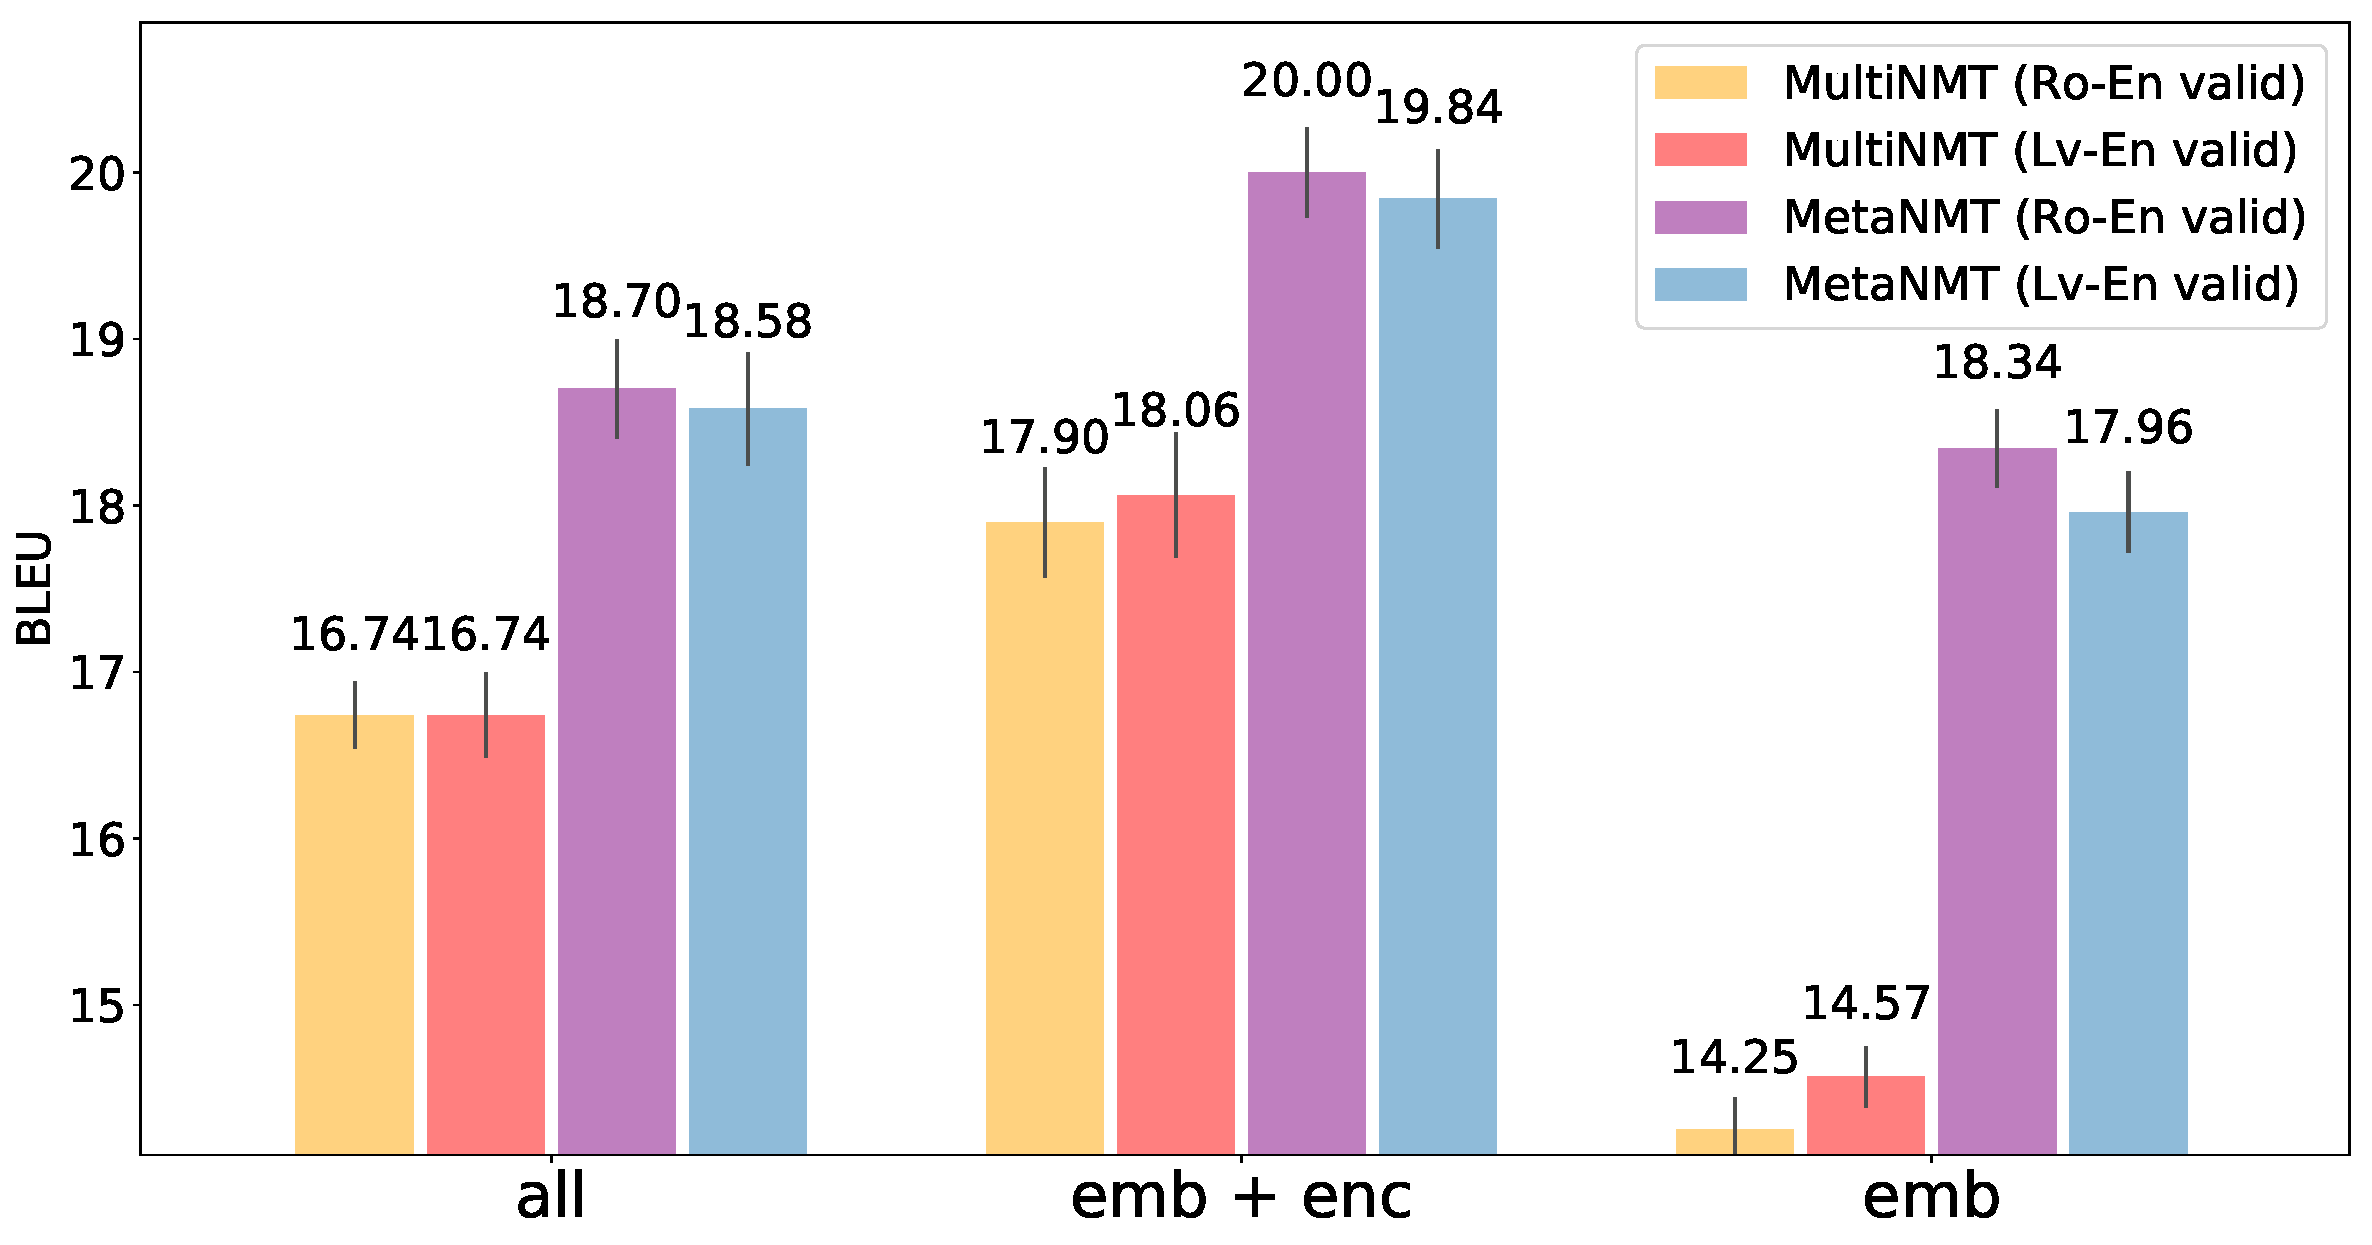
\includegraphics[width=\linewidth]{figs/meta/ro-en.pdf}              
\end{minipage}}
\subfigure[Lv-En]{                   
\begin{minipage}[t]{0.48\linewidth}
\centering                                                          
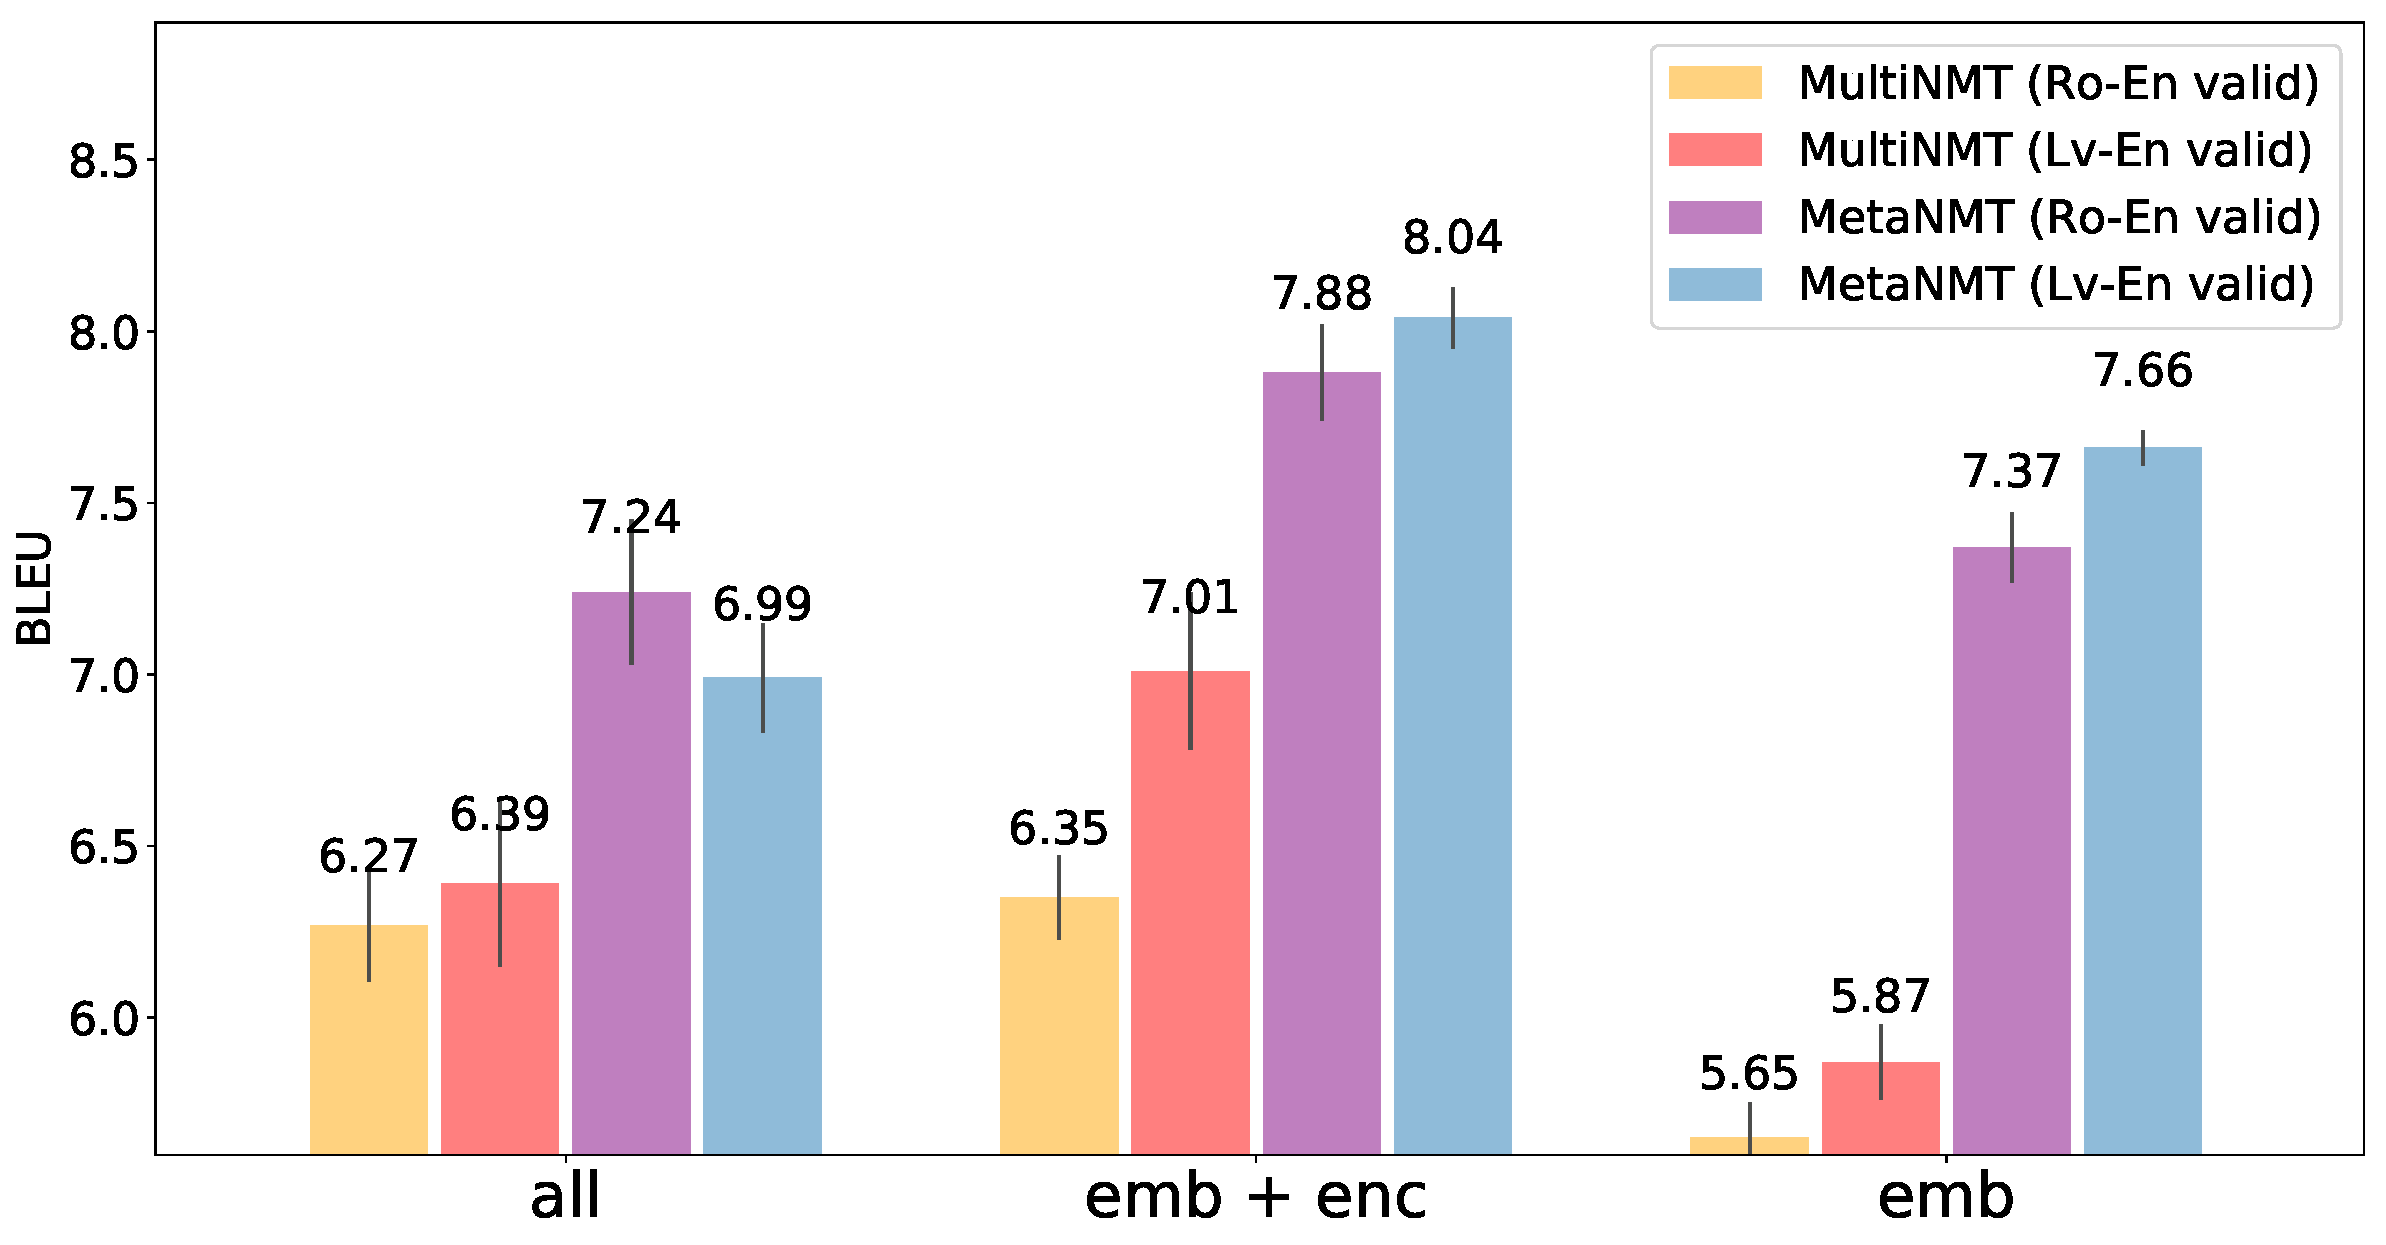
\includegraphics[width=\linewidth]{figs/meta/lv-en.pdf}                
\end{minipage}}
\subfigure[Fi-En]{                   
\begin{minipage}[t]{0.48\linewidth}
\centering                                                         
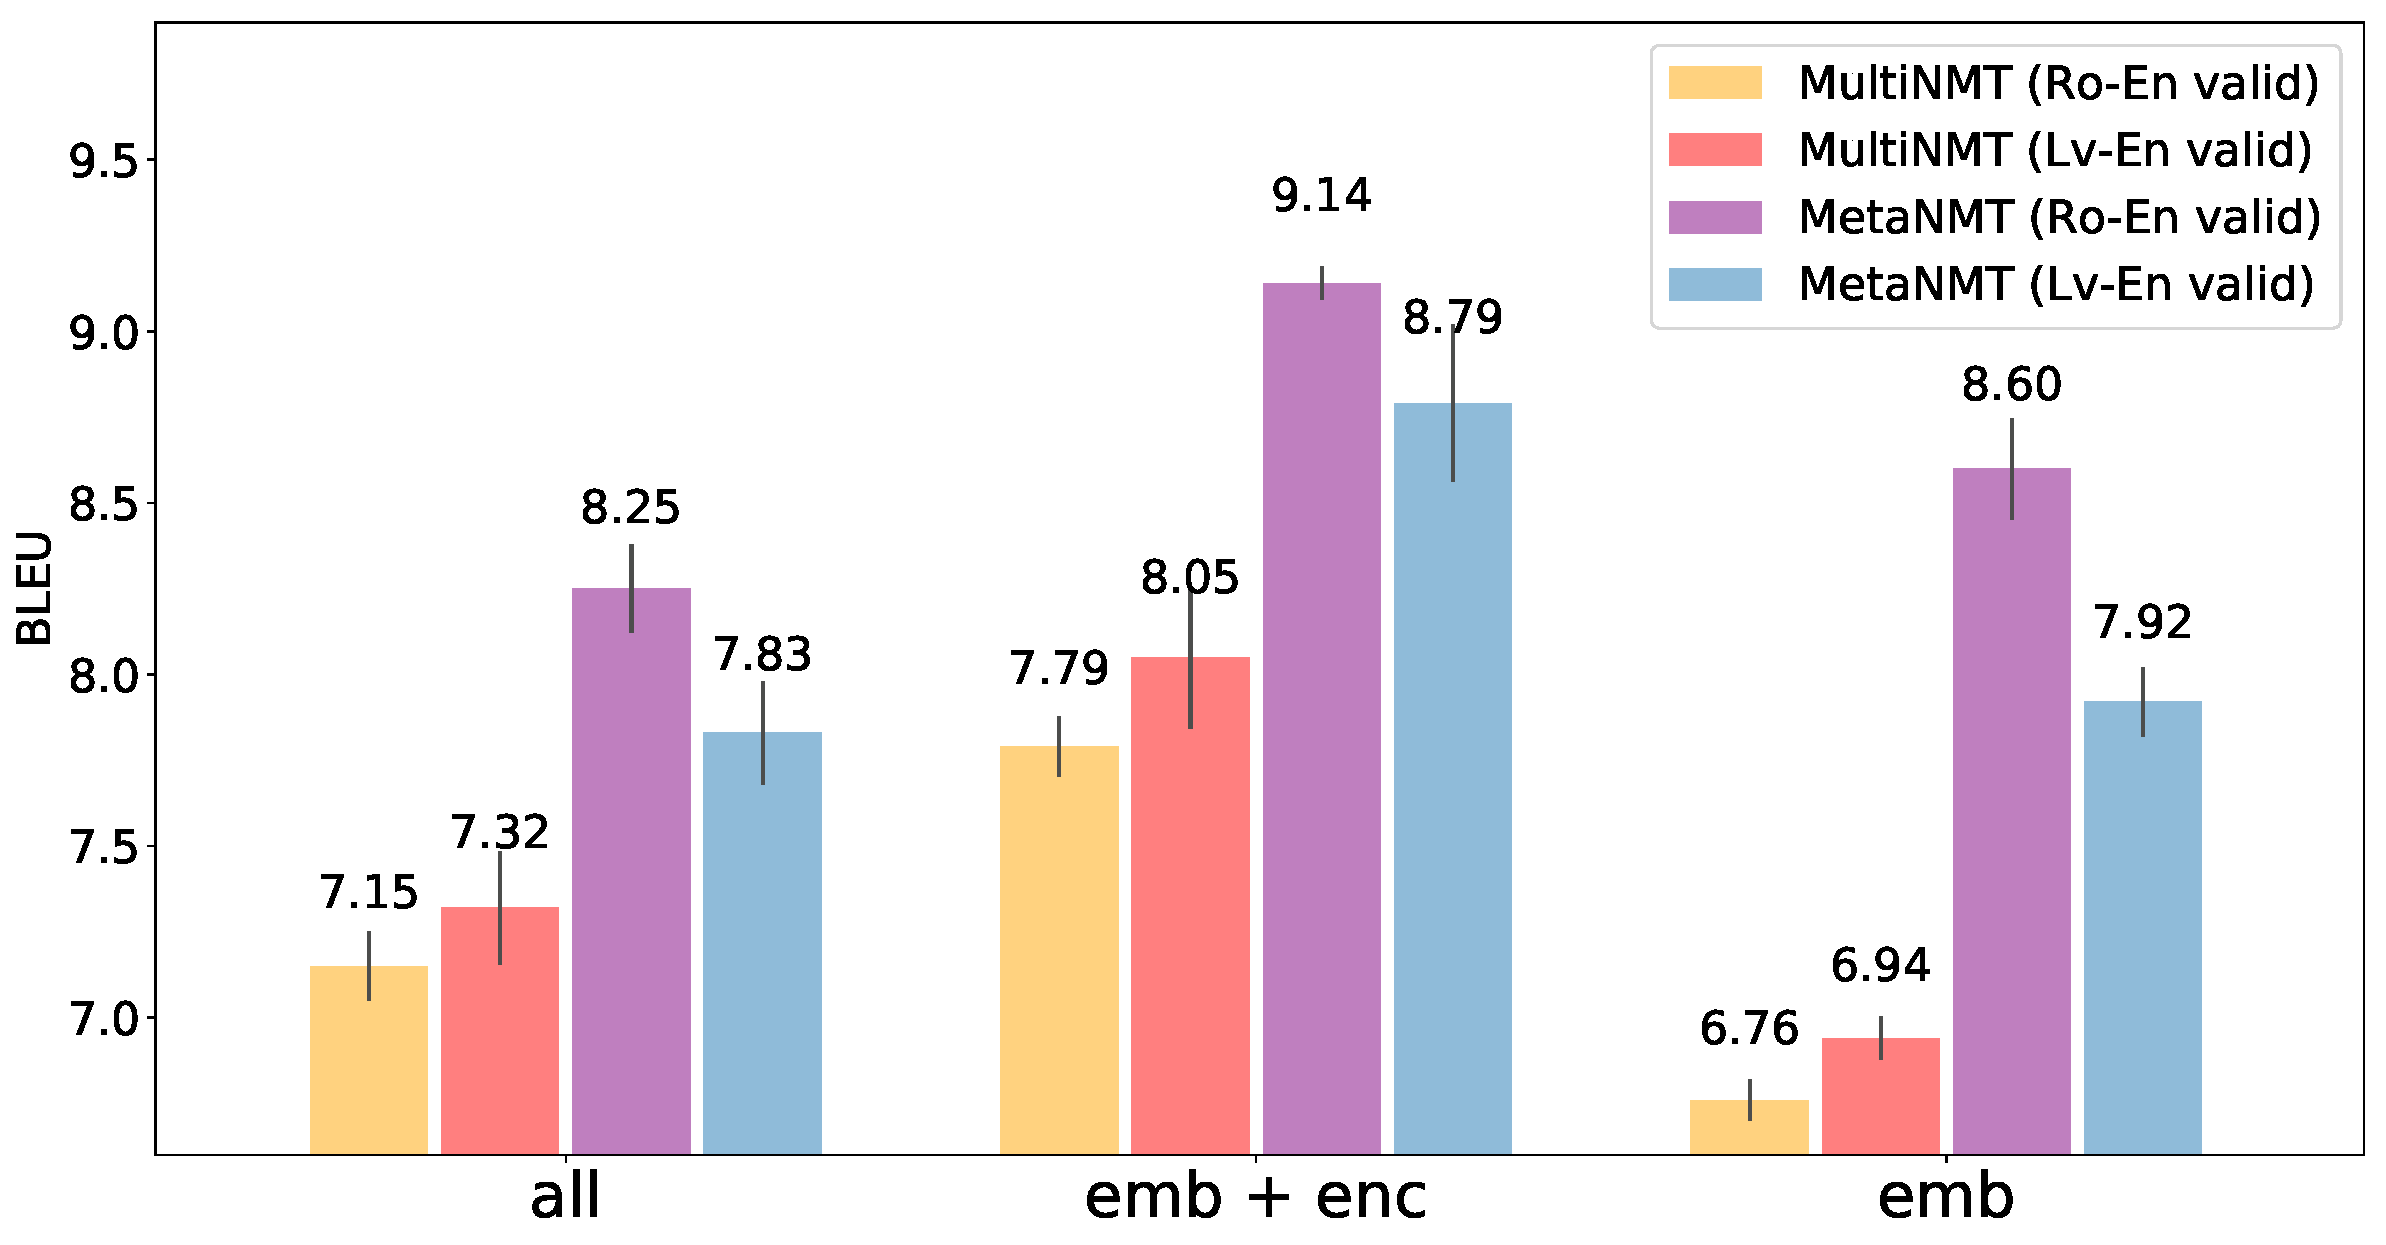
\includegraphics[width=\linewidth]{figs/meta/fi-en.pdf}              
\end{minipage}}
\subfigure[Tr-En]{                   
\begin{minipage}[t]{0.48\linewidth}
\centering                                                          
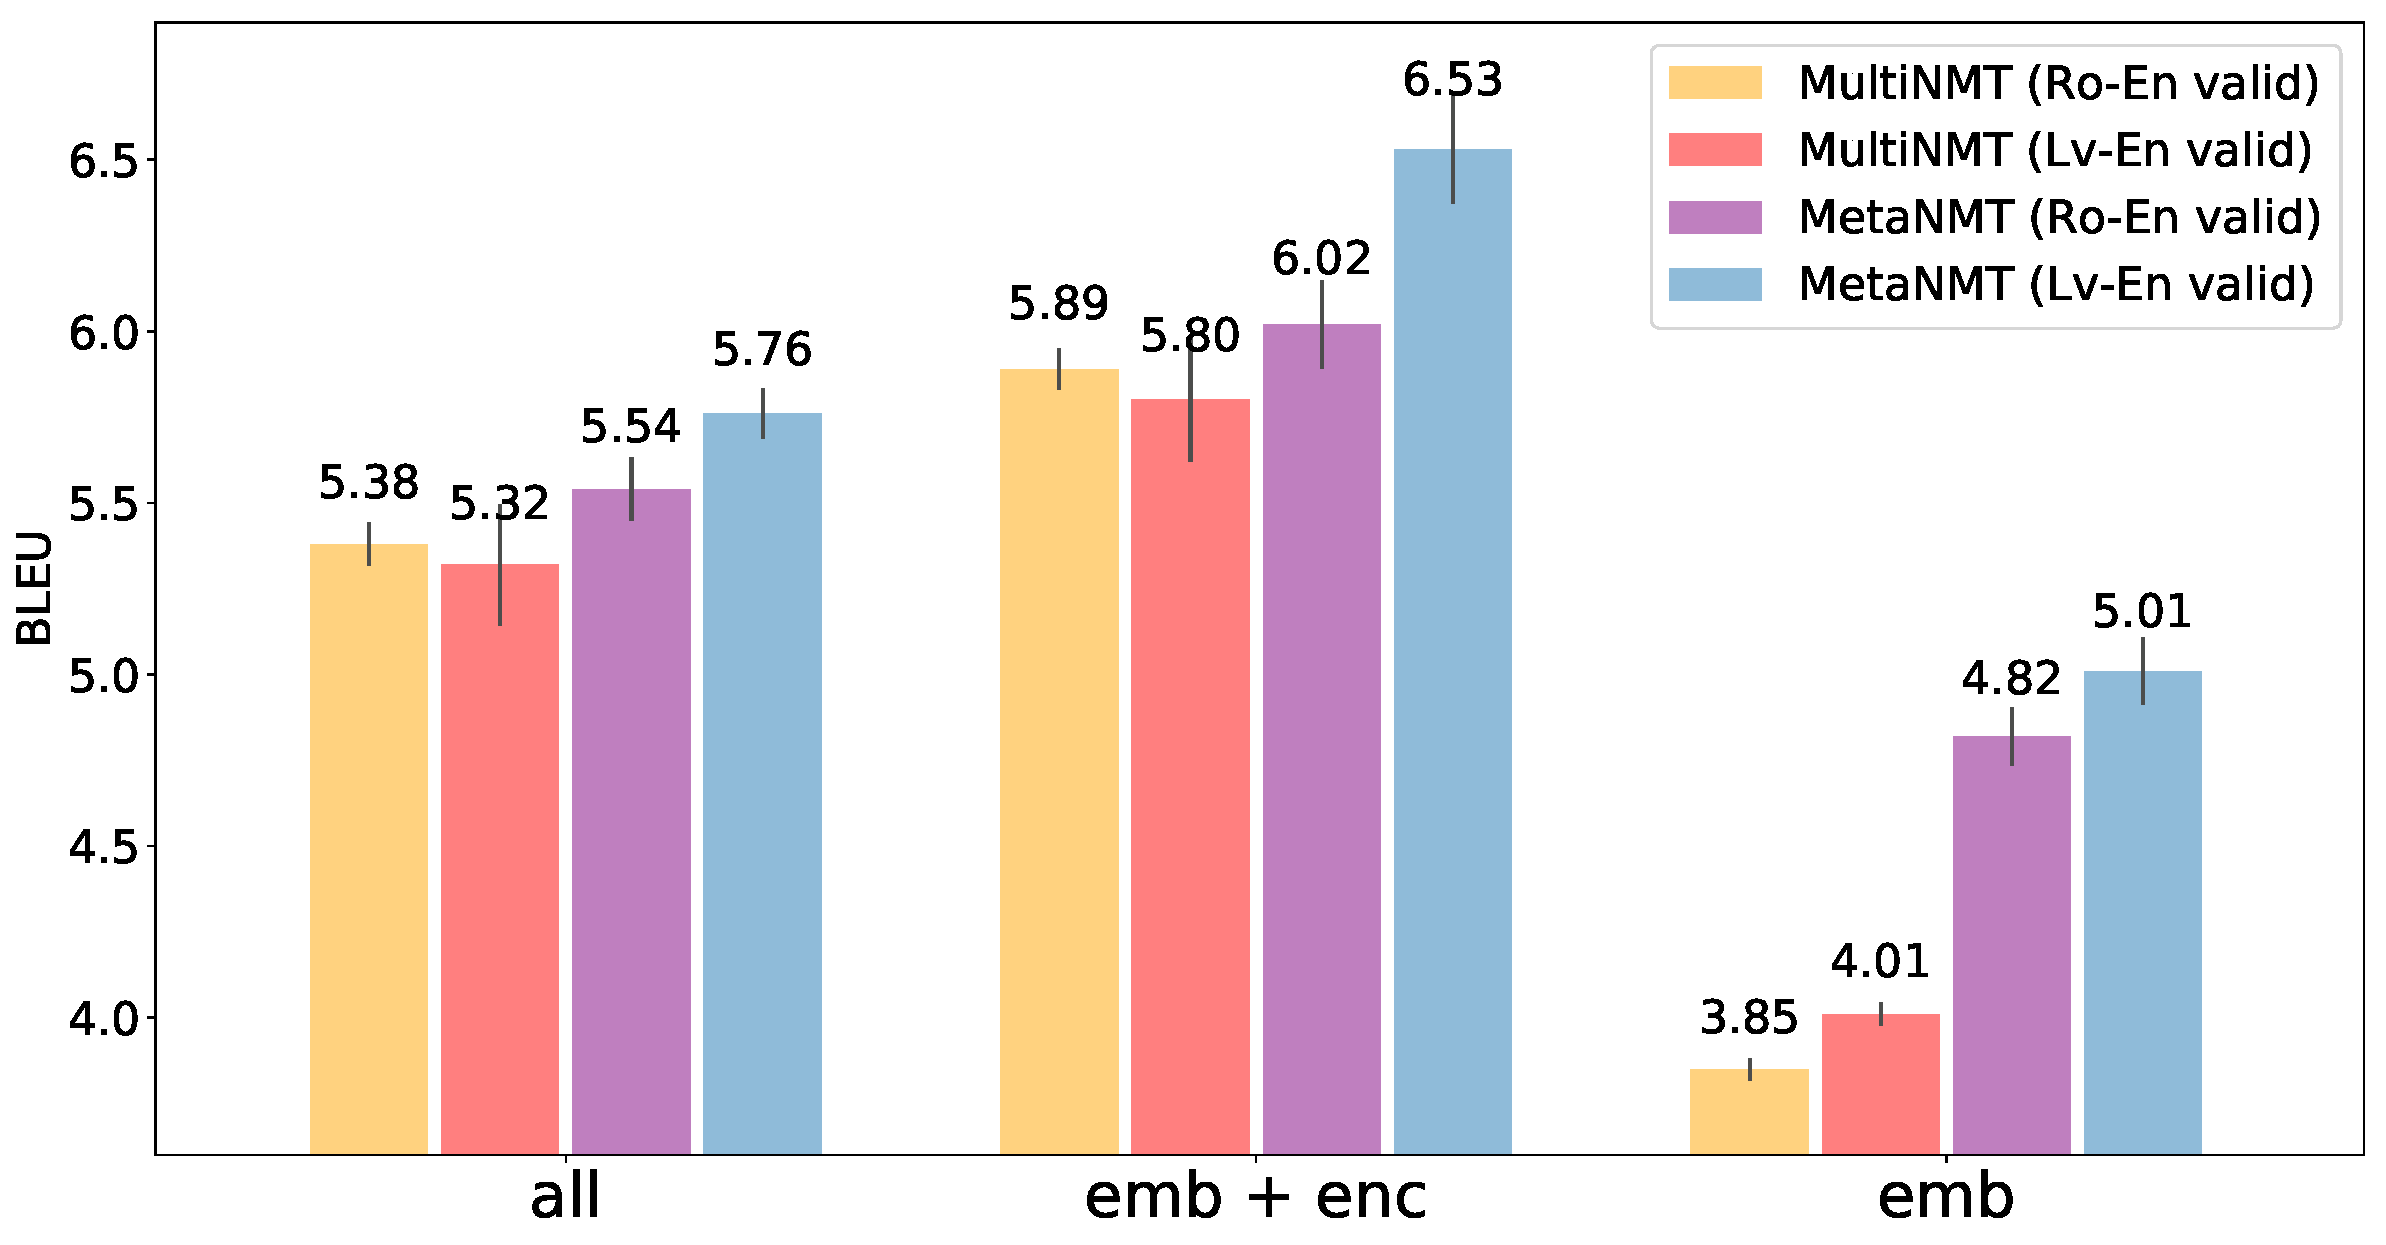
\includegraphics[width=\linewidth]{figs/meta/tr-en.pdf}                
\end{minipage}}
\caption{BLEU scores reported on test sets for \{Ro, Lv, Fi, Tr\} to En, where each model is first learned from 6 source tasks (Es, Fr, It, Pt, De, Ru) and then fine-tuned on randomly sampled training sets with around 16,000 English tokens per run. The error bars show the standard deviation calculated from 5 runs.} 
\label{cp6.fig.compare}                                                   
\end{figure*}

\paragraph{vs. Multilingual Transfer Learning}

We meta-learn the initial models on all the source tasks using either Ro-En or Lv-En as a validation task. We also train the initial models to be multilingual translation systems. We fine-tune them using the four target tasks (Ro-En, Lv-En, Fi-En and Tr-En; 16k tokens each) and compare the proposed meta-learning strategy and the multilingual, transfer learning strategy. As presented in Fig.~\ref{cp6.fig.compare}, the proposed learning approach significantly outperforms the multilingual, transfer learning strategy across all the target tasks regardless of which target task was used for early stopping. We also notice that the emb+enc strategy is most effective for both meta-learning and transfer learning approaches. With the proposed meta-learning and emb+enc fine-tuning, the final NMT systems trained using only a fraction of all available training examples achieve 2/3 (Ro-En) and 1/2 (Lv-En, Fi-En and Tr-En) of the BLEU score achieved by the models trained with full training sets.

\paragraph{Impact of Validation Tasks}

Similarly to training any other neural network, meta-learning still requires early-stopping to avoid overfitting to a specific set of source tasks. In doing so, we observe that the choice of a validation task has non-negligible impact on the final performance. For instance, as shown in Fig.~\ref{cp6.fig.compare}, Fi-En benefits more when Ro-En is used for validation, while the opposite happens with Tr-En. The relationship between the task similarity and the impact of a validation task must be investigated further in the future.
\begin{figure}[hptb]
    \centering
    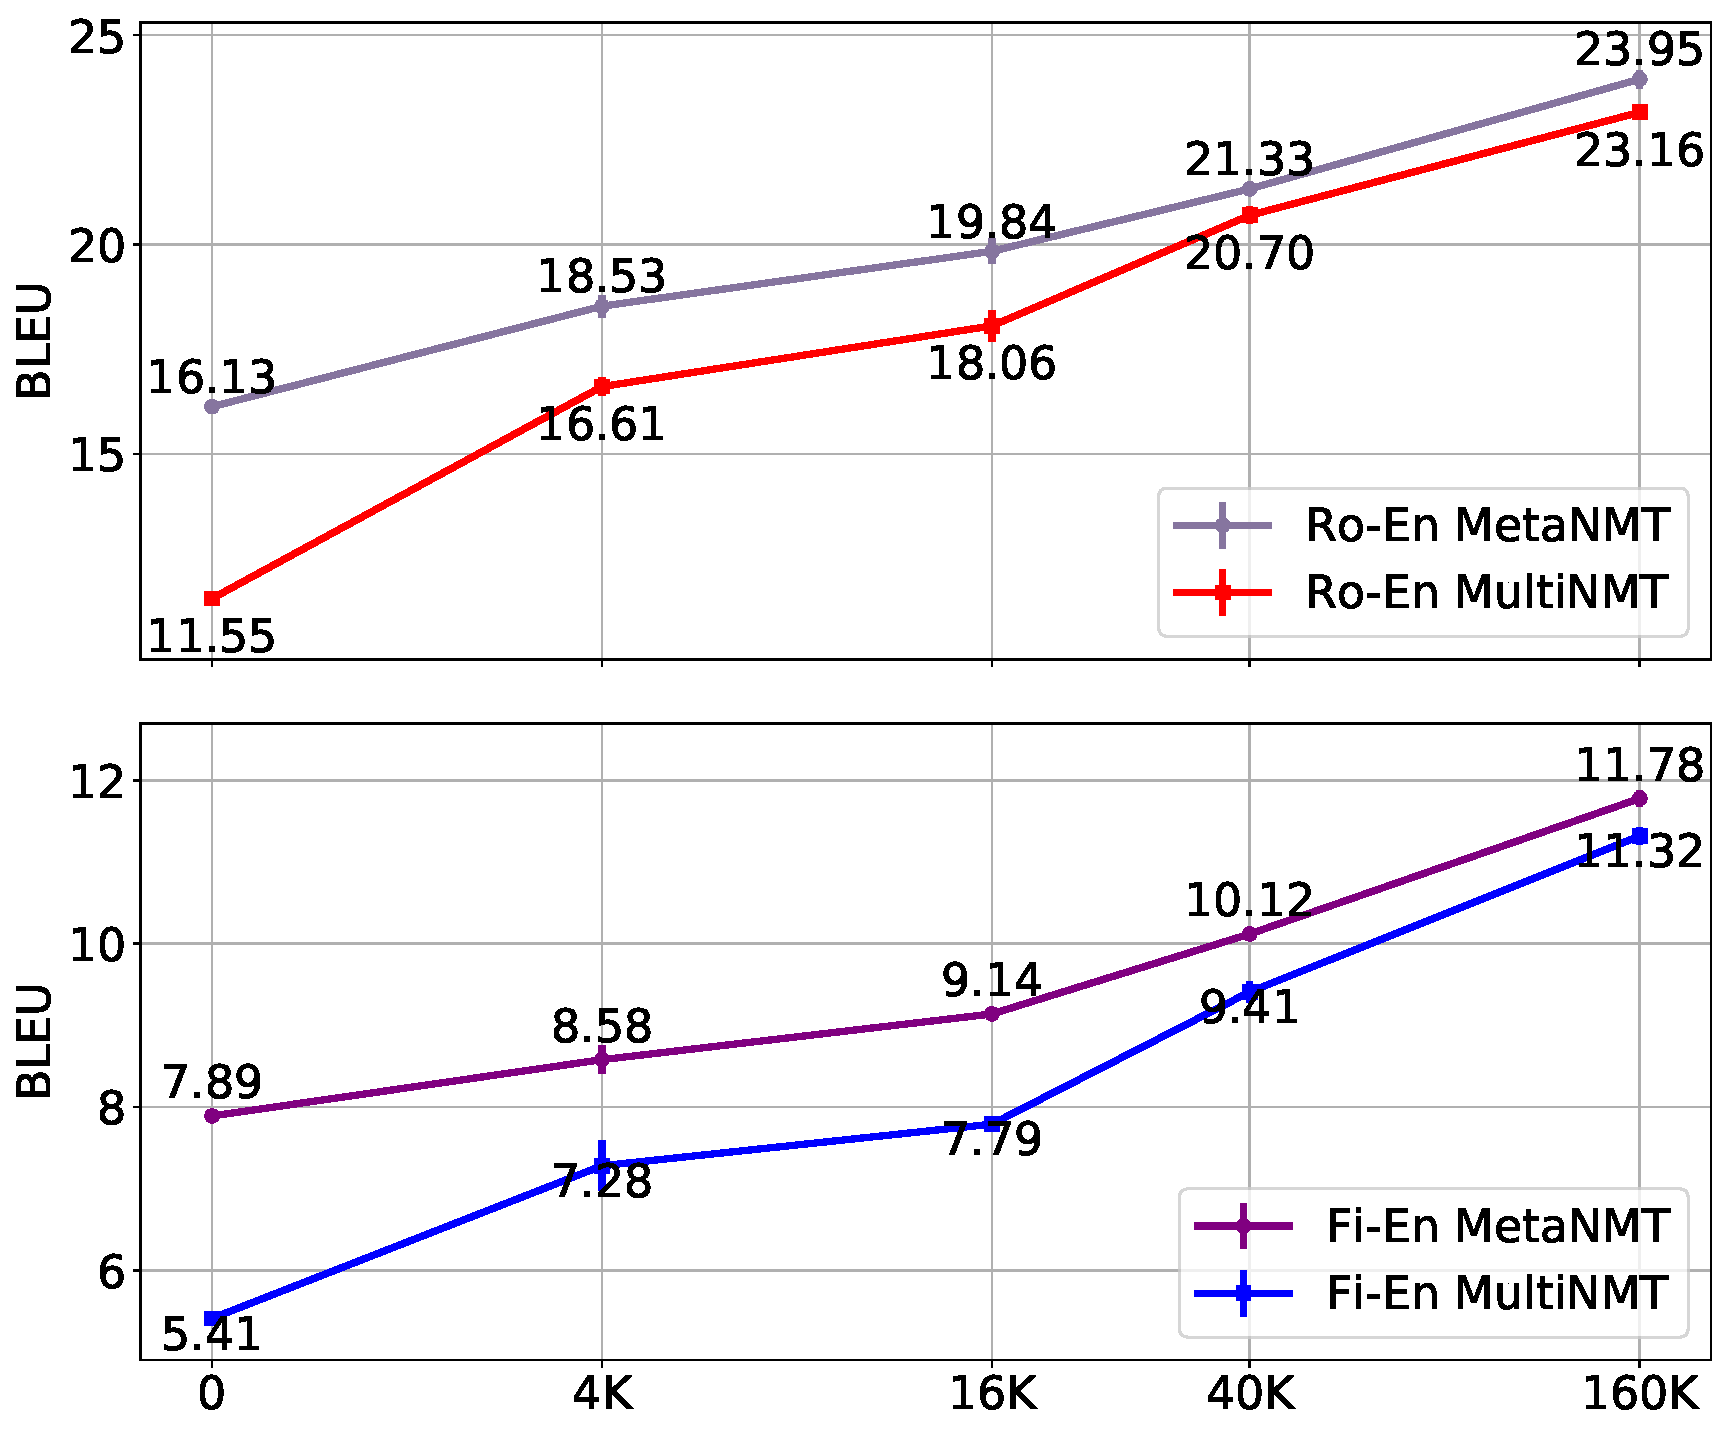
\includegraphics[width=0.8\linewidth]{figs/meta/support_size.pdf}
    \caption{BLEU Scores w.r.t. the size of the target task's training set.}
    \label{cp6.fig.support}
\end{figure}

% we also investigate the influence of using different languages as the validation task. 
% In general, 
% choosing the validation languages does have bias to the final performance on some target tasks, especially for the validation language itself and languages shares some similarities. For instance, the resulting BLEU scores of Fi-En with Ro as the validation task are higher in all the fine-tuning strategies of MetaNMT. In contrast, the performance on Tr-En does the opposite.

% Firstly, for training, choosing Lv-En as validation set benefits its performance other than a little drop of Tr-En in all and emb+enc finetune-tuning strategies. 
% For MetaNMT, its performance of choosing Ro-En as validation set is better than that of choosing Lv-En for Ro-En and Fi-En. However, Lv-En and Tr-En have the opposite results. 
% Secondly, we can see that the improvements of using different validation sets are different evidently. For Ro-En, Lv-En and Fi-En, the improvements of choosing Ro-En from MultiNMT to MetaNMT as validation set are greater than that of choosing Lv-En as validation set contrast to the opposite results for Tr-En.




% \begin{table}[tb]
% \centering
% \resizebox{0.48\textwidth}{!}{
% \begin{tabular}{rcc|rr}
% \toprule
% %  &\multicolumn{2}{c}{Bleu score}&\multicolumn{2}{c}{Bleu score}\\
% Model & Hessian Approx. & Inner steps & BLEU  & Speed\\
% \midrule
% \multirow{2}{*}{MetaNMT} 
% & & & & \\
% & & 1& & \\
% & & 2& & \\
% \bottomrule
% \end{tabular}
% }
% \caption{Performance and training speed comparison of variant options during meta-learning.}
% \label{table:ablation}
% \end{table}


\paragraph{Training Set Size}

We vary the size of the target task's training set and compare the proposed meta-learning strategy and multilingual, transfer learning strategy. We use the emb+enc fine-tuning on Ro-En and Fi-En. Fig.~\ref{cp6.fig.support} demonstrates that the meta-learning approach is more robust to the drop in the size of the target task's training set. The gap between the meta-learning and transfer learning grows as the size shrinks, confirming the effectiveness of the proposed approach on extremely low-resource language pairs.

\begin{figure}[htpb]
    \centering
    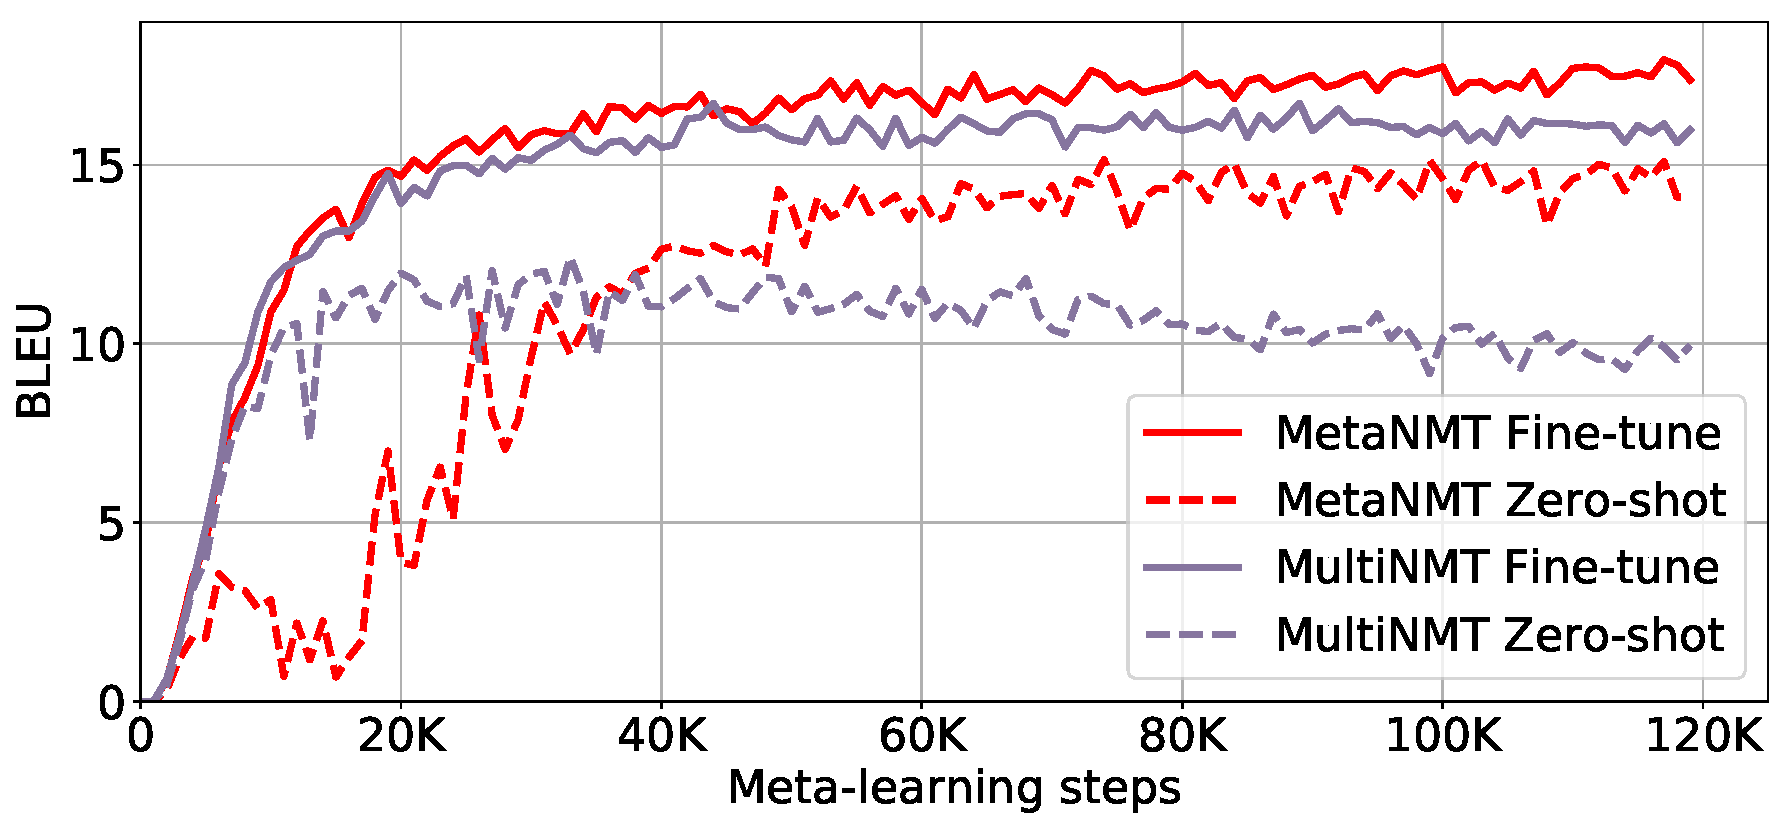
\includegraphics[width=0.8\linewidth]{figs/meta/curve.pdf}
    \caption{The learning curves of BLEU scores on the validation task (Ro-En).}%\alert{which target language pair?}}
    \label{cp6.fig.train_curve}
\end{figure}

\begin{sidewaystable}[hptb]
\centering
\resizebox{\textheight}{!}{
\begin{tabular}{l|cc|cc|cc|cc|cc}
\toprule
\multirow{2}{*}{Meta-Train} &  \multicolumn{2}{c|}{Ro-En} & \multicolumn{2}{c|}{Lv-En} & \multicolumn{2}{c|}{Fi-En} & \multicolumn{2}{c|}{Tr-En} & \multicolumn{2}{c}{Ko-En}\\
& zero & finetune & zero & finetune &  zero & finetune & zero & finetune & zero & finetune \\
\midrule
$-$                               &&$00.00 \pm .00$& & $0.00 \pm .00$  &  &$0.00 \pm .00$ & &$0.00 \pm .00$ & &$0.00 \pm .00$\\
Es                                &$9.20$&$15.71 \pm .22$& $2.23$& $4.65 \pm .12$  &  $2.73$&$5.55 \pm .08$ & $1.56$&$4.14 \pm .03$ & $0.63$&$1.40 \pm .09$\\
Es Fr                             &$12.35$&$17.46 \pm .41$& $2.86$& $5.05 \pm .04$  &  $3.71$&$6.08 \pm .01$ & $2.17$&$4.56 \pm .20$ & $0.61$&$1.70 \pm .14$ \\
Es Fr It Pt                       &$13.88$&$18.54 \pm .19$& $3.88$& $5.63 \pm .11$  &  $4.93$&$6.80 \pm .04$ & $2.49$&$4.82 \pm .10$ & $0.82$&$1.90 \pm .07$\\
\quad \quad \quad \quad\, De Ru   &$10.60$&$16.05 \pm .31$& $5.15$& $7.19 \pm .17$  &  $6.62$&$7.98 \pm .22$ & $3.20$&$6.02 \pm .11$ & $1.19$&$2.16 \pm .09$ \\
Es Fr It Pt De Ru                 &$15.93$&$20.00 \pm .27$& $6.33$& $7.88 \pm .14$  &  $7.89$&$9.14 \pm .05$ & $3.72$&$6.02 \pm .13$ & $1.28$&$2.44 \pm .11$ \\
All                &$18.12$&$\bm{22.04 \pm .23}$& $9.58$& $\bm{10.44 \pm .17}$ &  $11.39$&$\bm{12.63 \pm .22}$ & $5.34$ &$\bm{8.97 \pm .08}$ & $1.96$&$\bm{3.97 \pm .10}$ \\
\midrule
Full Supervised                   & \multicolumn{2}{c|}{$31.76$}& \multicolumn{2}{c|}{$15.15$} & \multicolumn{2}{c|}{$20.20$} & \multicolumn{2}{c|}{$13.74$} & \multicolumn{2}{c}{$5.97$}\\
\bottomrule
\end{tabular}
}
\caption{\label{cp6.table.aux}
BLEU Scores w.r.t. the source task set for all five target tasks.}
\end{sidewaystable}
\begin{table*}[hptb]
\centering
\small
%\resizebox{\textwidth}{!}{
\begin{tabular}{p{0.1\textwidth}|p{0.81\textwidth}}
\toprule
Source (Tr) & google \textcolor{blue}{mülteciler} için 11 milyon dolar \textcolor{purple}{toplamak} üzere bağış eşleştirme \textcolor{orange}{kampanyasını} \textcolor{red}{başlattı} .\\
Target & google \textcolor{red}{launches} donation-matching \textcolor{orange}{campaign} to \textcolor{purple}{raise} \$ 11 million for \textcolor{blue}{refugees} .\\
%Multi & \\
Meta-0 & google \textcolor{blue}{refugee} \textcolor{purple}{fund} for usd 11 million has \textcolor{red}{launched} a \textcolor{orange}{campaign} for donation .\\
Meta-16k & google has \textcolor{red}{launched} a \textcolor{orange}{campaign} to \textcolor{purple}{collect} \$ 11 million for \textcolor{blue}{refugees} . \\
\midrule
Source (Ko) & 이번에 체포되어 기소된 사람들 중에는 퇴역한 군 고위관리 , 언론인 , 정치인 , 경제인 등이 \textcolor{blue}{포함됐다} \\
Target & \textcolor{blue}{among} the suspects \textcolor{blue}{are} retired military officials , journalists , politicians , businessmen and others .\\
%Multi & \\
Meta-0 & last year , convicted people , among other people , of a high-ranking army of journalists in economic and economic policies , \textcolor{blue}{were included} . \\
Meta-16k & the arrested persons \textcolor{blue}{were included} in the charge , \textcolor{blue}{including} the military officials , journalists , politicians and economists .\\
% \midrule
% \midrule
% Source (Ro) & astfel , lucrarile de consolidare a cladirii ar putea fi reluate cel mai devreme anul viitor .\\
% Target & thus , the consolidation of the building could resume as early as next year .\\
% Multi & thus , building building building building building building could be resumed before next year .\\
% %Meta-0 & \\
% Meta-16k & thus , the building of the building could therefore be resumed as early as next year .\\
\bottomrule
\end{tabular}
%}
\caption{\label{cp6.table.example}
Sample translations for Tr-En and Ko-En highlight the impact of fine-tuning which results in syntactically better formed translations. We highlight tokens of interest in terms of reordering.
}
% KC: the last example is not too informative. a similar issue would be easily found with any kind of translation system.
% In the last example, we 
% Tr-En and Ko-En compare the difference of zero-shot and finetune, while Ro-En compares the difference of MetaNMT and MultiNMT. The same color denotes the same meanings.}
\end{table*}



\paragraph{Impact of Source Tasks}
In Table~\ref{cp6.table.aux}, we present the results on all five target tasks obtained while varying the source task set. We first see that it is always beneficial to use more source tasks. Although the impact of adding more source tasks varies from one language to another, there is up to 2$\times$ improvement going from one source task to 18 source tasks (Lv-En, Fi-En, Tr-En and Ko-En). The same trend can be observed even without any fine-tuning (i.e., unsupervised translation, \citep{lample2017unsupervised,artetxe2017unsupervised}). In addition, the choice of source languages has different implications for different target languages. For instance, Ro-En benefits more from \{Es, Fr, It, Pt\} than from \{De, Ru\}, while the opposite effect is observed with all the other target tasks. 


\paragraph{Training Curves}

The benefit of meta-learning over multilingual translation is clearly demonstrated when we look at the training curves in Fig.~\ref{cp6.fig.train_curve}. With the multilingual, transfer learning approach, we observe that training rapidly saturates and eventually degrades, as the model overfits to the source tasks. MetaNMT on the other hand continues to improve and never degrades, as the meta-objective ensures that the model is adequate for fine-tuning on target tasks rather than for solving the source tasks.

\paragraph{Sample Translations}
We present some sample translations from the tested models in Table~\ref{cp6.table.example}. Inspecting these examples provides the insight into the proposed meta-learning algorithm. For instance, we observe that the meta-learned model without any fine-tuning produces a word-by-word translation in the first example (Tr-En), which is due to the successful use of the universal lexcial representation and the meta-learned initialization. The system however cannot reorder tokens from Turkish to English, as it has not seen any training example of Tr-En. After seeing around 600 sentence pairs (16K English tokens), the model rapidly learns to correctly reorder tokens to form a better translation. A similar phenomenon is observed in the Ko-En example. These cases could be found across different language pairs.  


% Then, we can see that MetaNMT outperforms MultiNMT evidently in qualitative results. For example, for Ro-En, MetaNMT can translate this sentence properly comforming to English grammar and using suitable words and phrases while MultiNMT fails to do this.







% \subsection{Quantitative Comparison}

% We first conduct the experiments and evaluate the performance of metaNMT and multilingual transfer learning (MultiNMT) with a fixed training set which consists of six source tasks: Es Fr It Pt De Ru. Four target datasets (Ro Lv Fi Tr) with 16K En tokens are selected for the initial experiments.

% \paragraph{Overall performance}


% \paragraph{Fine-tuning St}
% Following \cite{zoph2016transfer}, fine-tuning different modules is investigated, namely finetune all, freeze decoder and only finetune embedding. Freeze decoder means that we finetune embedding and encoder. The main results are shown in Fig. \ref{cp6.fig.compare}. Here, we use the language sentences pairs which have $16,000$ En tokens. Firstly, it is very obvious that MetaNMT outperforms MultiNMT in all language pairs and finetune different modules. Secondly, when we only finetune encoder embedding, the improvements are the best among the three schemes of fine-tuning different modules. Especially, for Ro-En, MetaNMT can improve from $14.25$ to $18.34$ for Ro-En valication. Thirdly, the choice of validation set is very important and it affects the results greatly. If we use Ro-En as validation set, the improvements will be greater than choose Lv-En as validation set.  Fourthly, for different language pair, the improvements of performance are different. For Tr-En, the improvements are very small contrast to the great improvements for Ro-En.  
% \paragraph{v.s. support size}
% We also investigate the improvements as the increase of size of support sets. The results are shown in Fig. \ref{cp6.fig.support}. Firstly, we can see that when the size of support sets increases, the performance of MetaNMT and MultiNMT will increase. Secondly, when the size of support sets is very small, MetaNMT outperforms MultiNMT greatly. Especially, for Ro-En, when the size of support sets is $0$, MetaNMT can improve the performance from $11.55$ to $16.13$ than MultiNMT. Thirdly, when the size of support sets increases to a certain amount, the performance of MetaNMT and MultiNMT will have almost no difference. However, the performance of MetaNMT is always better than MultiNMT. For different language pairs, the observed results are the same.





% \paragraph{v.s. meta-learn languages}
% We also investigate the influence of using different language pairs in meta-train. The results are shown in Table \ref{cp6.table.aux}. Firstly, when more language pairs are added to the meta-train languages, the performance of both zero and finetune setting will increase. For example, after we add Fr to the source languages, the performance will be improved. When we use full Europarl and Ru as our meta-train dataset, the performance of finetune will achieve $22.04$ which has a very competitive performance contrast to full supervised setting. Secondly, for different target language pairs, different source language pairs will help them differently. For example, when the source languages change from Es Fr It Pt to De Ru, the performance of Ro-En drops from $18.54$ to $16.05$ while the performances of Lv-En, Fi-En, Tr-En and Ko-En all rise.



\section{Conclusion and Next Chapter}

In this chapter, we proposed a meta-learning algorithm for low-resource neural machine translation that exploits the availability of high-resource languages pairs. We based the proposed algorithm on the recently proposed model-agnostic meta-learning and adapted it to work with multiple languages that do not share a common vocabulary using the technique of universal lexcal representation, resulting in MetaNMT. Our extensive evaluation, using 18 high-resource source tasks and 5 low-resource target tasks, has shown that the proposed MetaNMT significantly outperforms the existing approach of multilingual, transfer learning in low-resource neural machine translation across all the language pairs considered.

The proposed approach opens new opportunities for neural machine translation. First, it is a principled framework for incorporating various extra sources of data, such as source- and target-side monolingual corpora. Second, it is a generic framework that can easily accommodate existing and future neural machine translation systems. 

Up to now we have basically introduced one direction of achieving a data-efficient neural machine translation system. From the next chapter, we will further investigate another important component of the existing NMT, i.e., decoding. We will first start to introduce a general learning framework -- {\it trainable decoding} --which can learn to build an efficient decoding in a principle way.

\part{Decoding-Efficient Neural Machine Translation}
\chapter[Trainable Greedy Decoding]{Trainable Greedy Decoding for Neural Machine Translation}
\label{trainable}
\section{Introduction}
\label{sec:introduction}

Neural machine translation has recently become a method of choice in machine translation research. Besides its success in traditional settings of machine translation, that is one-to-one translation between two languages, \citep{sennrich2016edinburgh,chung2016nyu}, neural machine translation has ventured into more sophisticated settings of machine translation. For instance, neural machine translation has successfully proven itself to be capable of handling subword-level representation of sentences \citep{lee2016fully,luong2016achieving,sennrich2015neural,costa2016character,ling2015character}. Furthermore, several research groups have shown its potential in seamlessly handling multiple languages \citep{dong2015multi,luong2015multi,firat2016multi,firat2016zero,lee2016fully,ha2016toward,viegas2016google}. 

A typical scenario of neural machine translation starts with training a model to maximize its log-likelihood. That is, we often train a model to maximize the conditional probability of a reference translation given a source sentence over a large parallel corpus. Once the model is trained in this way, it defines the conditional distribution over all possible translations given a source sentence, and the task of translation becomes equivalent to finding a translation to which the model assigns the highest conditional probability. Since it is computationally intractable to do so exactly, it is a usual practice to resort to approximate search/decoding algorithms such as greedy decoding or beam search. In this scenario, we have identified two points where improvements could be made. They are (1) training (including the selection of a model architecture) and (2) decoding.

% \begin{figure}[t]
% \centering
% 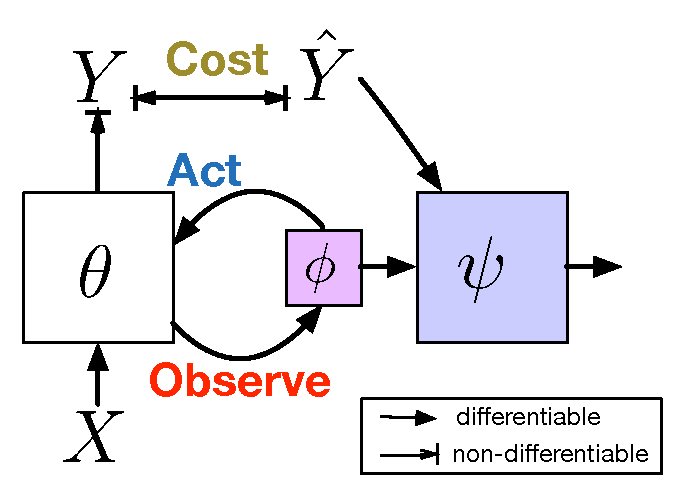
\includegraphics[width=0.85\linewidth]{figs/trainable/Concept.pdf}
% \caption{\label{fig:framework} The graphical illustration of the proposal trainable greedy decoding. $\theta$, $\phi$ and $\psi$ respectively correspond to the parameters of the underlying neural machine translation model, the trainable greedy decoding (actor) and the critic. 
% }
% \end{figure}

Much of the research on neural machine translation has focused solely on the former, that is, on improving the model architecture. Neural machine translation started with with a simple encoder-decoder architecture in which a source sentence is encoded into a single, fixed-size vector \citep{cho2014learning,sutskever2014sequence,kalchbrenner2013recurrent}. 
It soon evolved with the attention mechanism \citep{bahdanau2014neural}. 
A few variants of the attention mechanism, or its regularization, have been proposed recently to improve both the translation quality as well as the computational efficiency \citep{luong2015effective,cohn2016incorporating,tu2016modeling}. 
More recently, convolutional networks have been adopted either as a replacement of or a complement to a recurrent network in order to efficiently utilize parallel computing 
\citep{kalchbrenner2016neural,lee2016fully,gehring2016convolutional}.

On the aspect of decoding, only a few research groups have tackled this problem by incorporating a target decoding algorithm into training. \citet{wiseman2016sequence} and \citet{shen2015minimum} proposed a learning algorithm tailored for beam search. \citet{ranzato2015sequence} and \cite{bahdanau2016actor} suggested to use a reinforcement learning algorithm by viewing a neural machine translation model as a policy function.
Investigation on decoding alone has, however, been limited. \citet{cho2016noisy} showed the limitation of greedy decoding by simply injecting unstructured noise into the hidden state of the neural machine translation system. \citet{tu2016neural} similarly showed that the exactness of beam search does not correlate well with actual translation quality, and proposed to augment the learning cost function with reconstruction to alleviate this problem. \citet{li2016simple} proposed a modification to the existing beam search algorithm to improve its exploration of the translation space. 

In this paper, we tackle the problem of decoding in neural machine translation by introducing a concept of {\it trainable greedy decoding}. Instead of manually designing a new decoding algorithm suitable for neural machine translation, we propose to learn a decoding algorithm with an arbitrary decoding objective. More specifically, we introduce a neural-network-based decoding algorithm that works on an already-trained neural machine translation system by observing and manipulating its hidden state. We treat such a neural network as an agent with a deterministic, continuous action and train it with a variant of the deterministic policy gradient algorithm \citep{silver2014deterministic}. 

We extensively evaluate the proposed trainable greedy decoding on four language pairs (En-Cs, En-De, En-Ru and En-Fi; in both directions) with two different decoding objectives; sentence-level BLEU and negative perplexity. By training such trainable greedy decoding using deterministic policy gradient with the proposed critic-aware actor learning, we observe that we can improve decoding performance with minimal computational overhead. Furthermore, the trained actors are found to improve beam search as well, suggesting a future research direction in extending the proposed idea of trainable decoding for more sophisticated underlying decoding algorithms.

\section{Background}

\subsection{Neural Machine Translation}

Neural machine translation is a special case of conditional recurrent language modeling, where the source and target are natural language sentences. Let us use $X=\left\{ x_1, \ldots, x_{T_s} \right\}$ and $Y=\left\{ y_1, \ldots, y_T \right\}$ to denote source and target sentences, respectively. Neural machine translation then models the target sentence given the source sentence as:
%\begin{align*}
$p(Y|X) = \prod_{t=1}^T p(y_t | y_{<t}, X)$.
%\end{align*}
Each term on the r.h.s. of the equation above is modelled as a composite of two parametric functions:
\begin{align*}
p(y_t|y_{<t}, X)\propto \exp\left(g\left(y_t, z_t; \theta_g\right)\right),
\end{align*}
where 
%\begin{align*}
$z_t = f(z_{t-1}, y_{t-1}, e_t(X; \theta_e); \theta_f)$.
%\end{align*}
$g$ is a read-out function that transforms the hidden state $z_t$ into the distribution over all possible symbols, and $f$ is a recurrent function that compresses all the previous target words $y_{<t}$ and the time-dependent representation $e_t(X; \theta_e)$ of the source sentence $X$. This time-dependent representation $e_t$ is often implemented as a recurrent network encoder of the source sentence coupled with an attention mechanism \citep{bahdanau2014neural}.

% Neural machine translation~\cite{sutskever2014sequence,cho2014learning,bahdanau2014neural} has recently achieved impressive improvement~\cite{wu2016google} compared to traditional statistical machine translation methods. Across different variants, the NMT model typically models the machine translation as a auto-regressive generative model. That is to say, given a source sequence $X=\{x_1, ..., x_{Ts}\}$, the distribution of a translation sequence $Y = \{y_1, ..., y_T\}$ can be computed as:
% \begin{equation}
% \label{eq.crnnlm}
% p(Y|X) = \prod_{t=1}^T p(y_t|y_{<t}, X)
% \end{equation}
% where the conditional probability is modeled as the composite of two parametric functions:
% \begin{equation}
% \label{eq.model}
% \begin{split}
% &p(y_t|y_{<t}, X)\propto \exp\left(g\left(y_t, z_t; \theta_g\right)\right) \\
% &z_t = f(z_{t-1}, y_{t-1}, e_t(X; \theta_e); \theta_f)
% \end{split}
% \end{equation}
% where $e_t(X; \theta_e)$ is a time-dependent feature of the source sentence $X$ extracted by, for instance, a bi-directional recurrent neural network (RNN) with attention mechanism~\cite{bahdanau2014neural}, or so-called an \textit{encoder}; $f$ is a \textit{decoder} which is usually modeled by a separate RNN and $z_t$ is the hidden states of the decoder at step $t$; $g$ is the energy function which maps the hidden states into a distribution over the vocabulary. $\theta_g$, $\theta_f$ and $\theta_e$ are the parameters for $g$, $f$ and the encoder respectively.


\paragraph{Maximum Likelihood Learning}

We train a neural machine translation model, or equivalently estimate the parameters $\theta_g$, $\theta_f$ and $\theta_e$, by maximizing the log-probability of a reference translation $\hat{Y}=\{\hat{y}_1, ..., \hat{y}_T\}$ given a source sentence. That is, we maximize the log-likelihood function:
\begin{align*}
J^{\text{ML}}(\theta_g, \theta_f, \theta_e) = \frac{1}{N} \sum_{n=1}^N \sum_{t=1}^{T_n} \log p_{\theta}(\hat{y}_t^n| \hat{y}_{<t}^n, X^n),
\end{align*}
given a training set consisting of $N$ source-target sentence pairs. It is important to note that this maximum likelihood learning does not take into account how a trained model would be used. Rather, it is only concerned with learning a distribution over all possible translations. 



\subsection{Decoding}

Once the model is trained, either by maximum likelihood learning or by any other recently proposed algorithms \citep{wiseman2016sequence,shen2015minimum,bahdanau2016actor,ranzato2015sequence}, we can let the model translate a given sentence by finding a translation that maximizes 
\begin{align*}
\hat{Y} = \argmax_{Y} \log p_{\theta} (Y|X),
\end{align*}
where $\theta=(\theta_g, \theta_f, \theta_e)$.
This is, however, computationally intractable, and it is a usual practice to resort to approximate decoding algorithms.

\paragraph{Greedy Decoding}

One such approximate decoding algorithm is greedy decoding. In greedy decoding, we follow the conditional dependency path and pick the symbol with the highest conditional probability so far at each node. This is equivalent to picking the best symbol one at a time from left to right in conditional language modelling. A decoded translation of greedy decoding is $\hat{Y} = (\hat{y}_1, \ldots, \hat{y}_T)$, where
\begin{equation}
\hat{y}_t =  \argmax_{y \in V} \log p_{\theta}(y|\hat{y}_{<t}, X).
\end{equation}
Despite its preferable computational complexity $O(|V| \times T)$, greedy decoding has been over time found to be undesirably sub-optimal.% (see, e.g., \citep{cho2016noisy}.) 

\paragraph{Beam Search}  

Beam search keeps $K > 1$ hypotheses, unlike greedy decoding which keeps only a single hypothesis during decoding. At each time step $t$, beam search picks $K$ hypotheses with the highest scores ($\prod_{t'=1}^t p(y_t | y_{<t}, X)$). When all the hypotheses terminate (outputting the end-of-the-sentence symbol), it returns the hypothesis with the highest log-probability. Despite its superior performance compared to greedy decoding, the computational complexity grows linearly w.r.t. the size of beam $K$, which makes it less preferable especially in the production environment.


% \paragraph{\textbf{Training \& Testing Mismatch}} There is clearly a mismatch between the conventional pipeline. The NMT model is trained as a stochastic 

% \paragraph{\textbf{Metric Mismatch}} The target of maximum likelihood mismatches the final sequence-level evaluation metrics, for instance BLEU score in machine translation. That is to say, even if we can find a good decoding trajectory based on the trained conditional language model $\theta$, it still does not guarantee to obtain the best BLEU score in the end. 

\section{Trainable Greedy Decoding}

\subsection{Many Decoding Objectives}

Although we have described decoding in neural machine translation as a maximum-a-posteriori estimation in $\log p(Y|X)$, this is not necessarily the only %decoding objective 
nor the desirable decoding objective. 

First, each potential scenario in which neural machine translation is used calls for a unique decoding objective. In simultaneous translation/interpretation, which has recently been studied in the context of neural machine translation \citep{gu2016learning}, the decoding objective is formulated as a trade-off between the translation quality and delay. On the other hand, when a machine translation system is used as a part of a larger information extraction system, it is more important to correctly translate named entities and events than to translate syntactic function words. The decoding objective in this case must account for how the translation is used in subsequent modules in a larger system. 

Second, the conditional probability assigned by a trained neural machine translation model does not necessarily reflect our perception of translation quality. Although \citet{cho2016noisy} provided empirical evidence of high correlation between the log-probability and BLEU, a {\it de facto} standard metric in machine translation, there have also been reports on large mismatch between the log-probability and BLEU. For instance, \citet{tu2016neural} showed that beam search with a very large beam, which is supposed to find translations with better log-probabilities, suffers from pathological translations of very short length, resulting in low translation quality. This calls for a way to design or {\it learn} a decoding algorithm with an objective that is more directly correlated to translation quality. 

In short, there is a significant need for designing multiple decoding algorithms for neural machine translation, regardless of how it was trained. It is however non-trivial to manually design a new decoding algorithm with an arbitrary objective. This is especially true with neural machine translation, as the underlying structure of the decoding/search process -- the high-dimensional hidden state of a recurrent network -- is accessible but not interpretable. Instead, in the remainder of this section, we propose our approach of {\it trainable greedy decoding}.

\begin{figure*}[t]
\centering
\begin{minipage}{\textwidth}
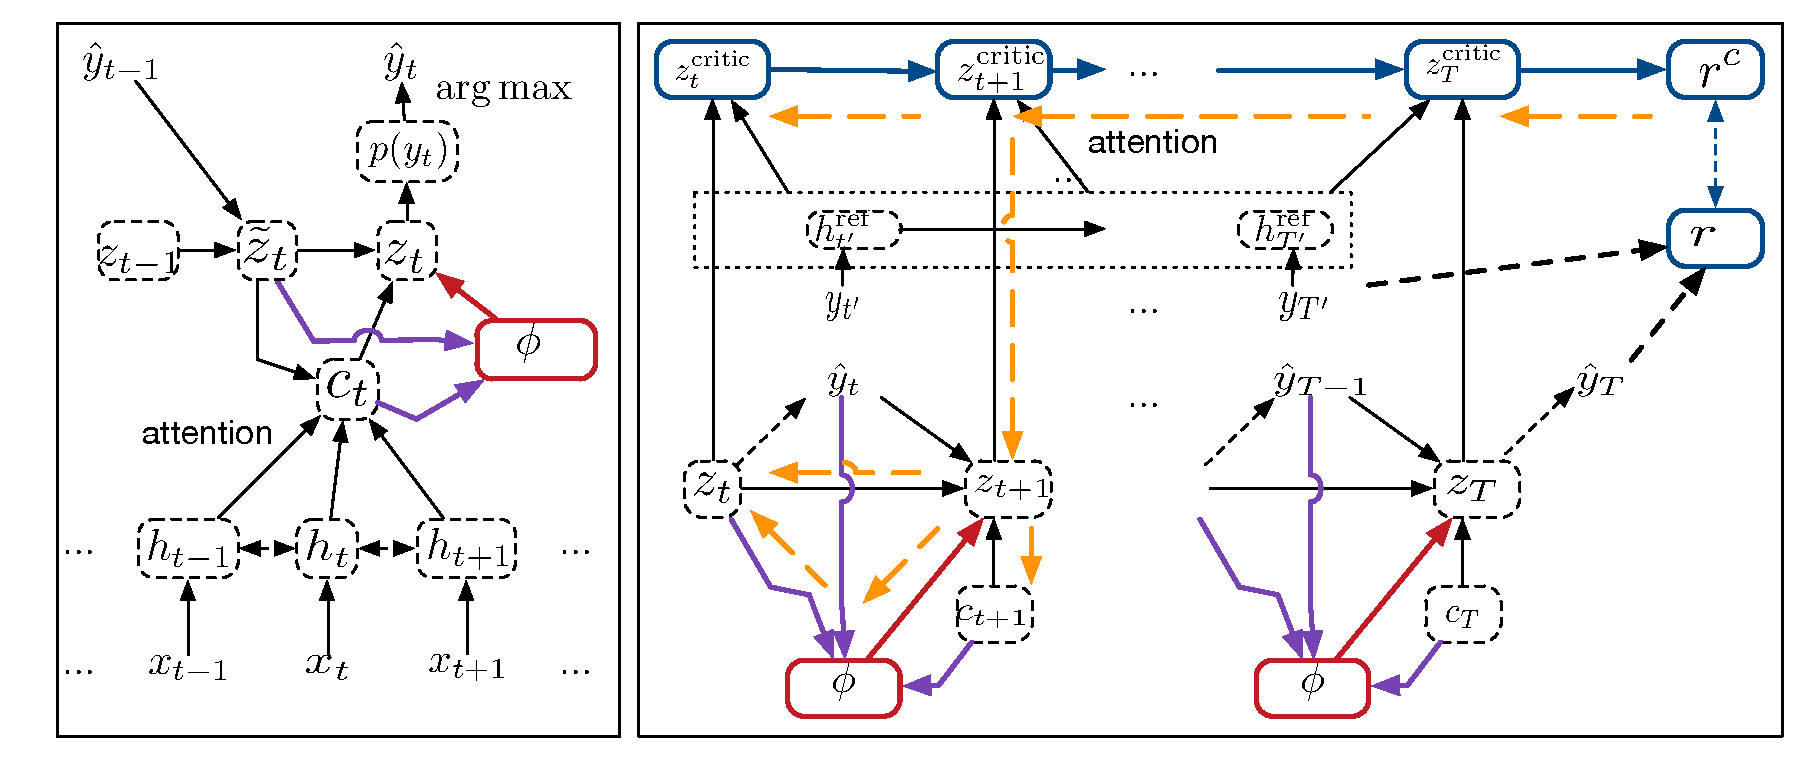
\includegraphics[width=\columnwidth]{figs/trainable/framework.pdf}
\vspace{-4mm}
\caption{\label{fig:tgd}  
Graphical illustrations of the trainable greedy decoding. The left panel shows a single step of the actor interacting with the underlying neural translation model, and The right panel the interaction among the underlying neural translation system (dashed-border boxes), actor (red-border boxes), and critic (blue-border boxes). The solid arrows indicate the forward pass, and the dashed yellow arrows the actor's backward pass. The dotted-border box shows the use of a reference translation.}
\end{minipage}
% \hfill
% \begin{minipage}{0.30\textwidth}
% \caption{\label{fig:tgd}  
% \small Graphical illustrations of the trainable greedy decoding. The left panel shows a single step of the actor interacting with the underlying neural translation model, and The right panel the interaction among the underlying neural translation system (dashed-border boxes), actor (red-border boxes), and critic (blue-border boxes). The solid arrows indicate the forward pass, and the dashed yellow arrows the actor's backward pass. The dotted-border box shows the use of a reference translation.}
% \end{minipage}
\vspace{-1mm}
\end{figure*}

\subsection{Trainable Greedy Decoding}

We start from the noisy, parallel approximate decoding (NPAD) algorithm proposed in \citep{cho2016noisy}. The main idea behind NPAD algorithm is that a better translation with a higher log-probability may be found by injecting unstructured noise in the transition function of a recurrent network. That is,
\begin{align*}
z_t = f(z_{t-1} + \epsilon_t, y_{t-1}, e_t(X; \theta_e); \theta_f),
\end{align*}
where $\epsilon_t \sim \mathcal{N}(0, (\sigma_0/t)^2)$. NPAD avoids potential degradation of translation quality by running such a noisy greedy decoding process multiple times in parallel. An important lesson of NPAD algorithm is that there exists a decoding strategy with the asymptotically same computational complexity that results in a better translation quality, and that such a better translation can be found by manipulating the hidden state of the recurrent network. 

In this work, we propose to significantly extend NPAD by replacing the unstructured noise $\epsilon_t$ with a parametric function approximator, or an agent, $\pi_{\phi}$. This agent takes as input the previous hidden state $z_{t-1}$, previously decoded word $\hat{y}_{t-1}$ and the time-dependent context vector $e_t(X; \theta_e)$ and outputs a real-valued vectorial action $a_t \in \mathbb{R}^{\text{dim}(z_t)}$. Such an agent is trained such that greedy decoding with the agent finds a translation that maximizes any predefined, arbitrary decoding objective, while the underlying neural machine translation model is pretrained and fixed. Once the agent is trained, we generate a translation given a source sentence by greedy decoding however augmented with this agent. We call this decoding strategy {\it trainable greedy decoding}. 
%See Fig.~\ref{fig:framework} for a graphical illustration of the proposed idea of trainable greedy decoding.


% To replace a fixed decoding method, we proposed the trainable decoding framework that separately \textit{learns} the decoding criterion $Y = G_{\theta, \phi}(X)$ after training. More precisely, we focus on a trainable greedy decoding algorithm as follows,
% \begin{equation}
% \label{eq.actor}
%  y_t =  \argmax_{y \in V} \log p_{\theta, \phi}(y|y_{<t}, X)
% \end{equation}
% where $\theta$ is the trained NMT model, and $\phi$ is the additional parameters that can be optimized by any evaluation metric using reinforcement learning. 

% Note that the proposed framework differs from many previous efforts that incorporate reinforcement learning to fine-tune the entire NMT model for different targets~\cite{ranzato2015sequence,bahdanau2016actor}. In these cases, the NMT is treated as a stochastic policy of selecting words and still suffers the mismatch of training and testing. 
% In contrast, we treat the existing NMT model ($\theta$) as a fixed black-box and learn an actor ($\phi$) to control it. In detail, the actor is a neural network that directly interacts with the decoder RNN at each time step to control the decoded symbol. Therefore, the proposed algorithm does not make any assumption for decoding algorithm as well as the target to optimize (see details at~\ref{sec.model}). Ideally we can directly optimize the decoding without mismatch. 

% Generally, learning a model to output a high dimensional continuous control signal is extremely difficult. Targeting on the learning difficulty, a novel learning algorithm based on deterministic policy gradient and a critic-aware exploration algorithm will be discussed in detail at~\ref{sec.learn}.



\paragraph{Related Work: Soothsayer prediction function}

Independently from and concurrently with our work here, \citet{li2017learning} proposed, just two weeks earlier, to train a neural network that predicts an arbitrary decoding objective given a source sentence and a partial hypothesis, or a prefix of translation, and to use it as an auxiliary score in beam search. For training such a network, referred to as a Q network in their paper, they generate each training example by either running beam search or using a ground-truth translation (when appropriate) for each source sentence. This approach allows one to use an arbitrary decoding objective, but it still relies heavily on the log-probability of the underlying neural translation system in actual decoding. We expect a combination of these and our approaches may further improve decoding for neural machine translation in the future.

\subsection{Learning and Challenges}

While all the parameters---$\theta_g$, $\theta_f$ and $\theta_e$--- of the underlying neural translation model are fixed, we only update the parameters $\phi$ of the agent $\pi$. This ensures the generality of the pretrained translation model, and allows us to train multiple trainable greedy decoding agents with different decoding objectives, maximizing the utility of a single trained translation model. 

Let us denote by $R$ our arbitrary decoding objective as a function that scores a translation generated from trainable greedy decoding. Then, our learning objective for trainable greedy decoding is 
\begin{align*}
J^{\text{A}}(\phi) = \mathbb{E}_{X \sim D}^{\hat{Y}=G_{\pi}(X)}\left[R(\hat{Y})\right],
\end{align*}
where we used $G_{\pi}(X)$ as a shorthand for trainable greedy decoding with an agent $\pi$. 

There are two major challenges in learning an agent with such an objective. First, the decoding objective $R$ may not be differentiable with respect to the agent. Especially because our goal is to accommodate an arbitrary decoding objective, this becomes a problem. For instance, BLEU, a standard quality metric in machine translation, is a piece-wise linear function with zero derivatives almost everywhere. Second, the agent here is a real-valued, deterministic policy with a very high-dimensional action space (1000s of dimensions), which is well known to be difficult. In order to alleviate these difficulties, we propose to use a variant of the deterministic policy gradient algorithm \citep{silver2014deterministic,lillicrap2015continuous}.

\section{Deterministic Policy Gradient \\ with Critic-Aware Actor Learning}

\subsection{Deterministic Policy Gradient \\ for Trainable Greedy Decoding}

It is highly unlikely for us to have access to the gradient of an arbitrary decoding objective $R$ with respect to the agent $\pi$, or its parameters $\phi$. Furthermore, we cannot estimate it stochastically because our policy $\pi$ is defined to be deterministic without a predefined nor learned distribution over the action. Instead, following \citep{silver2014deterministic,lillicrap2015continuous}, we use a parametric, differentiable approximator, called a critic $R^c$, for the non-differentiable objective $R$. We train the critic by minimizing
\begin{align*}
J^{\text{C}}(\psi) = \mathbb{E}_{X \sim D}^{\hat{Y}=G_{\pi}(X)}\left[R^c_{\psi}(z_{1:T}) - R(\hat{Y})\right]^2.
\end{align*}
The critic observes the state-action sequence of the agent $\pi$ via the modified hidden states $(z_1, \ldots, z_T)$ of the recurrent network, and predicts the associated decoding objective. By minimizing the mean squared error above, we effectively encourage the critic to approximate the non-differentiable objective as closely as possible in the vicinity of the state-action sequence visited by the agent. 

We implement the critic $R^c$ as a recurrent network, similarly to the underlying neural machine translation system. This implies that we can compute the derivative of the predicted decoding objective with respect to the input, that is, the state-action sequence $z_{1:T}$, which allows us to update the actor $\pi$, or equivalently its parameters $\phi$, to maximize the predicted decoding objective. Effectively we avoid the issue of non-differentiability of the original decoding objective by working with its proxy. 

With the critic, the learning objective of the actor is now to maximize not the original decoding objective $R$ but its proxy $R^{\text{C}}$ such that
\begin{align*}
\hat{J}^{\text{A}}(\phi) = \mathbb{E}_{X \sim D}^{\hat{Y}=G_{\pi}(X)}\left[R^{\text{C}}(\hat{Y})\right].
\end{align*}
Unlike the original objective, this objective function is fully differentiable with respect to the agent $\pi$. We thus use a usual stochastic gradient descent algorithm to train the agent, while simultaneously training the critic. We do so by alternating between training the actor and critic. Note that we maximize the return of a full episode rather than the Q value, unlike usual approaches in reinforcement learning.







% \subsection{Actor}
% \label{sec.model}
% The actor $\phi$ is a controller (feed-forward or recurrent) neural network aside of the decoder RNN so that at each time step $t$, $\phi$ reads the state $z_t$ of the decoder, and outputs a deterministic continuous action vector $a_t$ into the decoder. For simplicity:
% \begin{equation}
% \tilde{z}_t = z_t \oplus a_t, \quad \quad a_t = \phi(z_t, a_{t-1})
% \end{equation}
% where we use $\tilde{z}_t$ to replace $z_t$ in Eq.~\ref{eq.model} to change the word distribution. $\oplus$ is utilized to show that this continuous action has additive property biasing the decoder's states, which is critical as this action does not only influence the current decoded words, but will also change the future trajectories.

% \paragraph{Internal Bias} Instead of directly adding the action $a_t$ onto the hidden states $z_t$ before read-out, we found that adding the control signal $a_t$ inside the RNN will consistently works better. As shown in Fig.~\ref{fig.internal}, the additive action will be pushed into a second gated recurrent unit~(GRU) to compute the actual hidden states. We believe that this internal action can change the states more effectively because of the non-linear structures. 
% % \begin{figure}[hptb]
% % \centering
% % 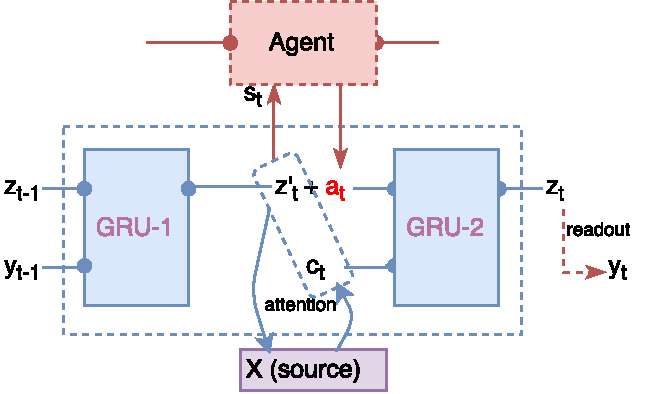
\includegraphics[width=\linewidth]{onestep.pdf}
% % \caption{\label{fig.internal} Injecting action as internal bias}
% % \end{figure}

% \paragraph{Objectives} The actor can be trained directly by optimizing any sequence-level reward, such as BLEU score or perplexity. In general, suppose $R(Y, \hat{Y})$ represents the objective evaluation metrics about the decoded translation $Y$ and the ground truth $\hat{Y}$. Note that $\hat{Y}$ does not necessarily been used to evaluate the generated translation $Y$, for instance, when the metric is using \textit{perplexity}.

% At each time step $t$, the word $y_t$ is decoded with greedy decoding from a actor-biased distribution based on Eq.~\ref{eq.actor}, and the decoding process is shown in Fig.~\ref{fig.internal}. Clearly, $y_t$ is depended on all historical actions $a_1, ..., a_t$ from the actor.
% % \begin{equation}
% % Y = \{y_1, ..., y_T\}, \ \ y_t =  \argmax_{y} \log \hat{p}(y_t=y|a_{\leq t}, y_{<t}, X), \\ a_t = A(s_t, a_{t-1}; \theta_A)
% % \end{equation}
% Thus, the target is to find the best actor $\phi$ so that maximizing the expectation of the rewards, that is
% \begin{equation}
% \label{eq.reward}
% J^{RL}(\phi) = \mathbb{E}_{X, \hat{Y}\sim D}^{Y=G_{\theta, \phi}(X)}\left[R(Y, \hat{Y})\right]
% \end{equation}

% \paragraph{Non-differentiability} Unfortunately, optimizing Eq.~\ref{eq.reward} with gradient-based methods is almost intractable as $G$ is non-differentiable w.r.t $\phi$ because of greedy decoding. Furthermore, in many cases, the true reward $R$ is also not differentiable to the input sequence, e.g. BLEU scores. Thirdly, directly optimize greedy decoding indicates that we cannot compute the exact distribution of $G(X)$ in order to use any score function based methods~\cite{bahdanau2016actor} to avoid non-differentiability.

% \subsection{Deterministic Policy Gradient}

% To solve the problem of non-differentiability, we adapt and utilize the deterministic policy gradient methods from~\cite{silver2014deterministic,lillicrap2015continuous}. More precisely, we introduce a critic $\psi$, a parametric, differentiable function that predicts $R^c$ to replace the reward $R$ in Eq.~\ref{eq.reward}. The actor is then adjusted to maximize the output of the critic. In practice, the critic is an RNN which takes the hidden states $z_1, ..., z_T$ of the decoder at each time step, and attends to the reference words $\hat{Y}$. The prediction is performed at last step after a nonlinear activation into real values.

% \paragraph{Learning $\bm{\phi}$} 
% Based on Eq.~\ref{eq.reward}, we can directly compute the gradient w.r.t the translation from the differentiable critic: $\partial R^c_{\psi}/\partial z_{1:T}$. Through this partial derivative, we can further compute the updating direction of the actor $\phi$ using the chain rule as:
% \begin{equation}
% \label{eq.chain}
%     \phi \leftarrow \phi + \eta 
%     \frac{\partial R^c_{\psi}}{\partial z_{1:T}} \frac{\partial z_{1:T}}{\partial
%     a_{1:T}} \frac{\partial a_{1:T}}{\partial \phi}.
% \end{equation}
% All the partial derivatives on the r.h.s. can be easily computed using the back-propagation. Once training is done, we discard the critic and keep only the actor as a final policy to control the greedy decoding algorithm.

% \paragraph{Learning $\bm{\psi}$} 
% On the other hand, the critic can be trained to minimize the square difference between the true reward and its prediction, that is to say:
% \begin{equation}
% \label{eq.critic}
% J^C(\psi) = \mathbb{E}_{X, \hat{Y}\sim D}^{Y=G_{\theta, \phi}(X)}\left[R^c_{\psi}(z_{1:T}, \hat{Y}) - R(Y, \hat{Y})\right]^2
% \end{equation}
% Note that we make the critic to approximate the full reward of each episode rather than a Q function in most existing reinforcement learning algorithms. The most important difference is in our case, we don't have to make any MDP assumption and we can directly optimize the episodic reward.

% Ideally, it is essential to train the critic until converge every time the actor is updated with Eq.~\ref{eq.chain} as in order to obtain a stable gradient estimation, we need make sure the critic approximates the changes of the true reward well w.r.t the actor. In practice, we alternate the training for both $\phi$ and $\psi$.


% \begin{figure}[hptb]
% \centering
% 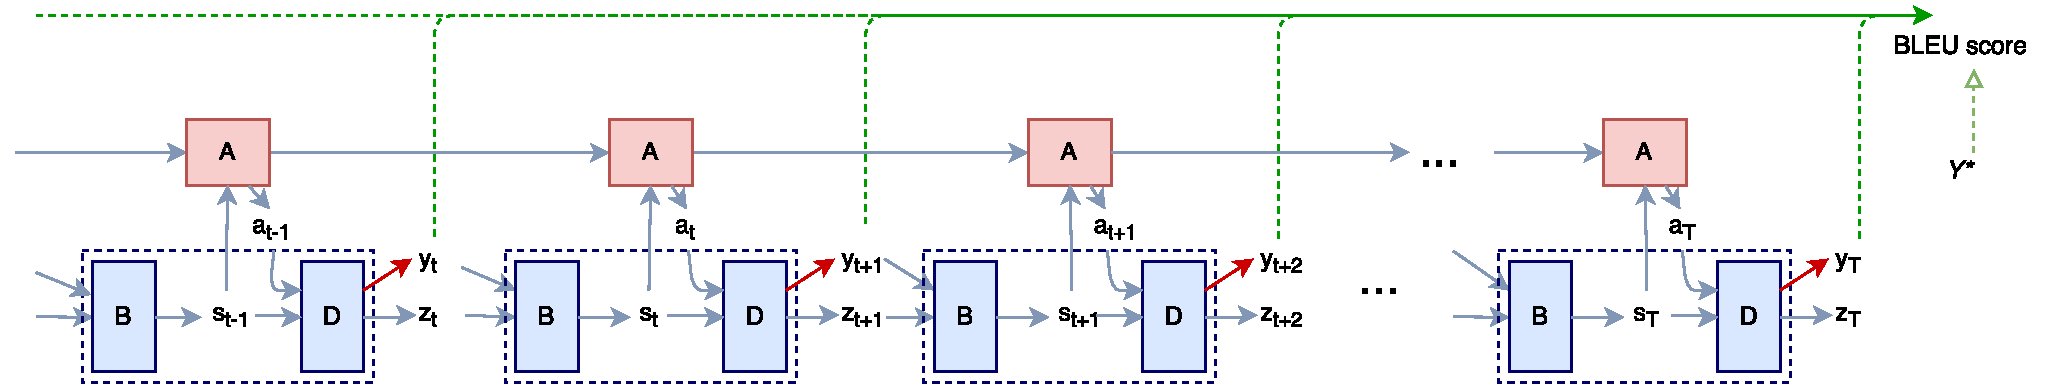
\includegraphics[width=\linewidth]{seq1.pdf}
% \caption{\label{fig.learning} Learning objectives}
% \end{figure}
%\label{sec.learn}

\begin{algorithm}[t]
\caption{Trainable Greedy Decoding}
\label{algo2}
\begin{algorithmic}[1]
\small
\Require{NMT $\theta$, actor $\phi$, critic $\psi$, $N_c$, $N_a$, $S_c$, $S_a$, $\tau$}
\State Train $\theta$ using MLE on training set $D$;
\State Initialize $\phi$ and $\psi$;
\State Shuffle $D$ twice into $D_{\phi}$ and $D_{\psi}$
\While{stopping criterion is not met}
\For{$t=1:N_c$}
\State Draw a translation pair: $(X, Y)\sim D_{\psi}$;
\State $r, r^c=\textsc{Decode}(S_c, X, Y, 1)$
\State Update $\psi$ using $\nabla_{\psi}\sum_k{\left(r_k^c - r_k\right)^2}/(S_c+1)$
\EndFor
\For{$t=1:N_a$}
\State Draw a translation pair: $(X, Y)\sim D_{\phi}$;
\State $r, r^c=\textsc{Decode}(S_a, X, Y, 0)$
\State Compute $w_k = \exp\left(-\left(r_k^c - r_k\right)^2/\tau\right)$
\State Compute $\tilde{w}_k=w_k/\sum_k{w_k}$
\State Update $\phi$ using $-\sum_k{\left(\tilde{w}_k\cdot \nabla_{\phi}r^c_k\right)}$
\EndFor
\EndWhile
\Statex{}
\setcounter{ALG@line}{0}
\Statex{\hspace{-18pt}\textbf{Function: }}{\textsc{Decode}$(S, X, Y, c)$}
  \State $Y_s = \{\}$, $Z_s = \{\}$, $r = \{\}$, $r^c=\{\}$;
  \For{$k=1:S$}
   \State Sample noise $\epsilon \sim \mathcal{N}(0, \sigma^2)$ for each action;
   \State Greedy decoding $\hat{Y}^{k} = G_{\theta, \phi}(X)$ with $\epsilon$;
   \State Collect hidden states $z^{k}_{1:T}$ given $X$, $\hat{Y}$, $\theta$, $\phi$
   \State $Y_s \leftarrow Y_s \cup \{Y^k\}$
   \State $Z_s \leftarrow Z_s \cup \{z^{k}_{1:T}\}$
  \EndFor
  \If{$c=1$}
   \State Collect hidden states $z_{1:T}$ given $X$, $Y$, $\theta$
   \State $Y_s \leftarrow Y_s \cup \{Y\}$
   \State $Z_s \leftarrow Z_s \cup \{ z_{1:T} \}$
  \EndIf
  \For{$\hat{Y}, Z \in Y_s, Z_s$} 
   \State Compute the critic output $r^c \leftarrow R^c_{\psi}(Z, \hat{Y})$ 
   \State Compute true reward $r \leftarrow R(Y, \hat{Y})$
  \EndFor
  \State \textbf{return} $r$, $r^c$
\end{algorithmic}
\end{algorithm}

\begin{figure*}[t]
\centering
\begin{minipage}{\textwidth}
\centering

  \begin{minipage}{0.48\columnwidth}
  \centering
  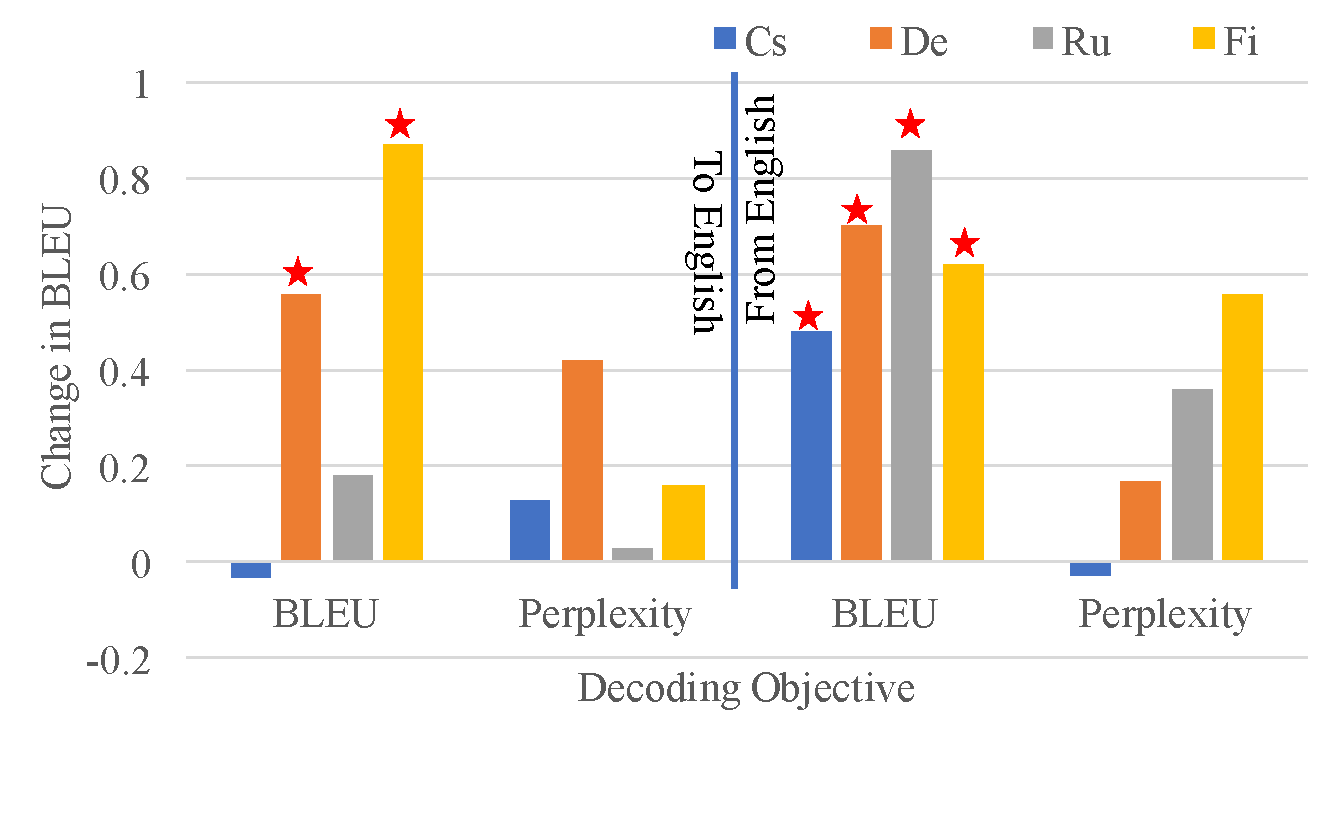
\includegraphics[width=\columnwidth]{figs/trainable/greedy_bleu.pdf}
  \end{minipage}
  \hfill
  \begin{minipage}{0.48\columnwidth}
  \centering
  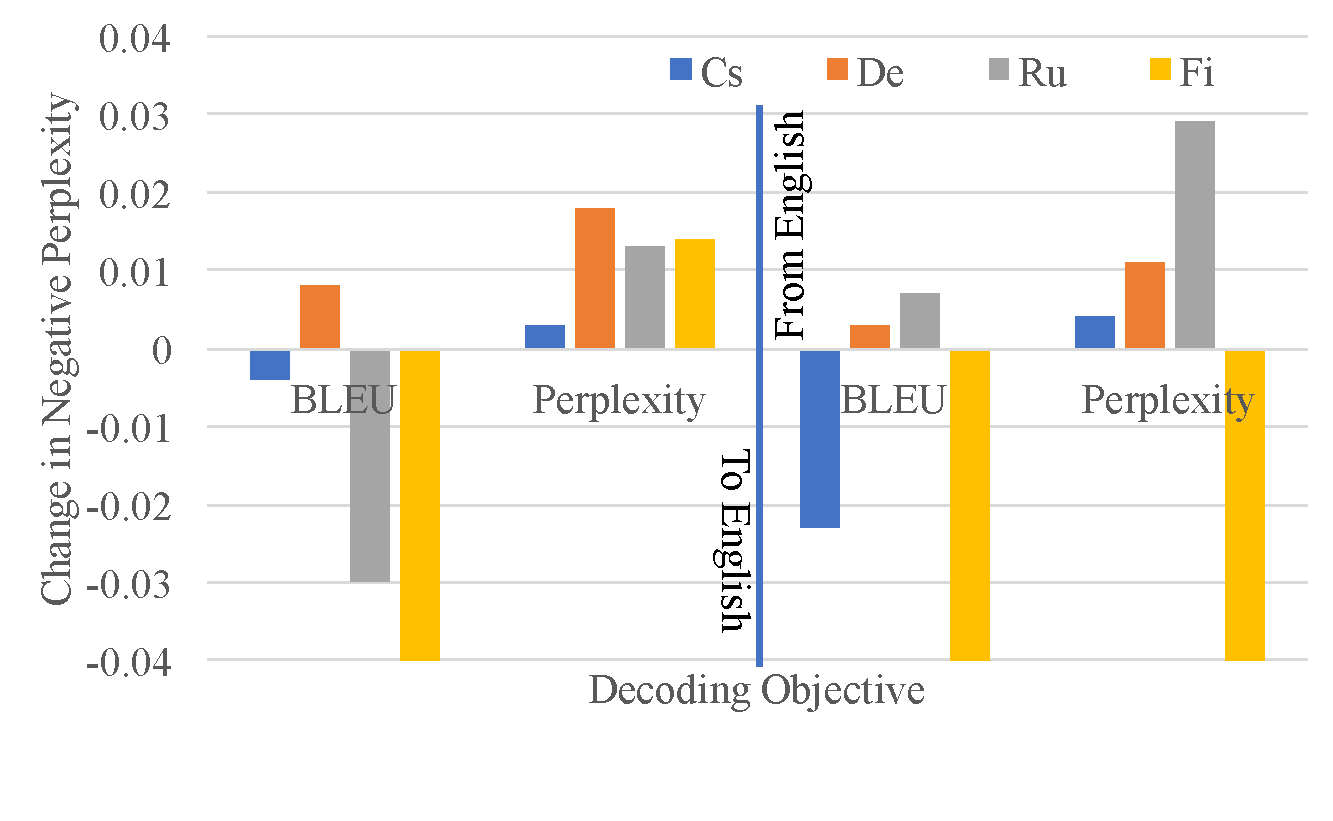
\includegraphics[width=\columnwidth]{figs/trainable/greedy_perplexity.pdf}
  \end{minipage}
  \label{fig:r1}

  %\vspace{-1mm}
  (a) Trainable Greedy Decoding

  \begin{minipage}{0.48\columnwidth}
  \centering
  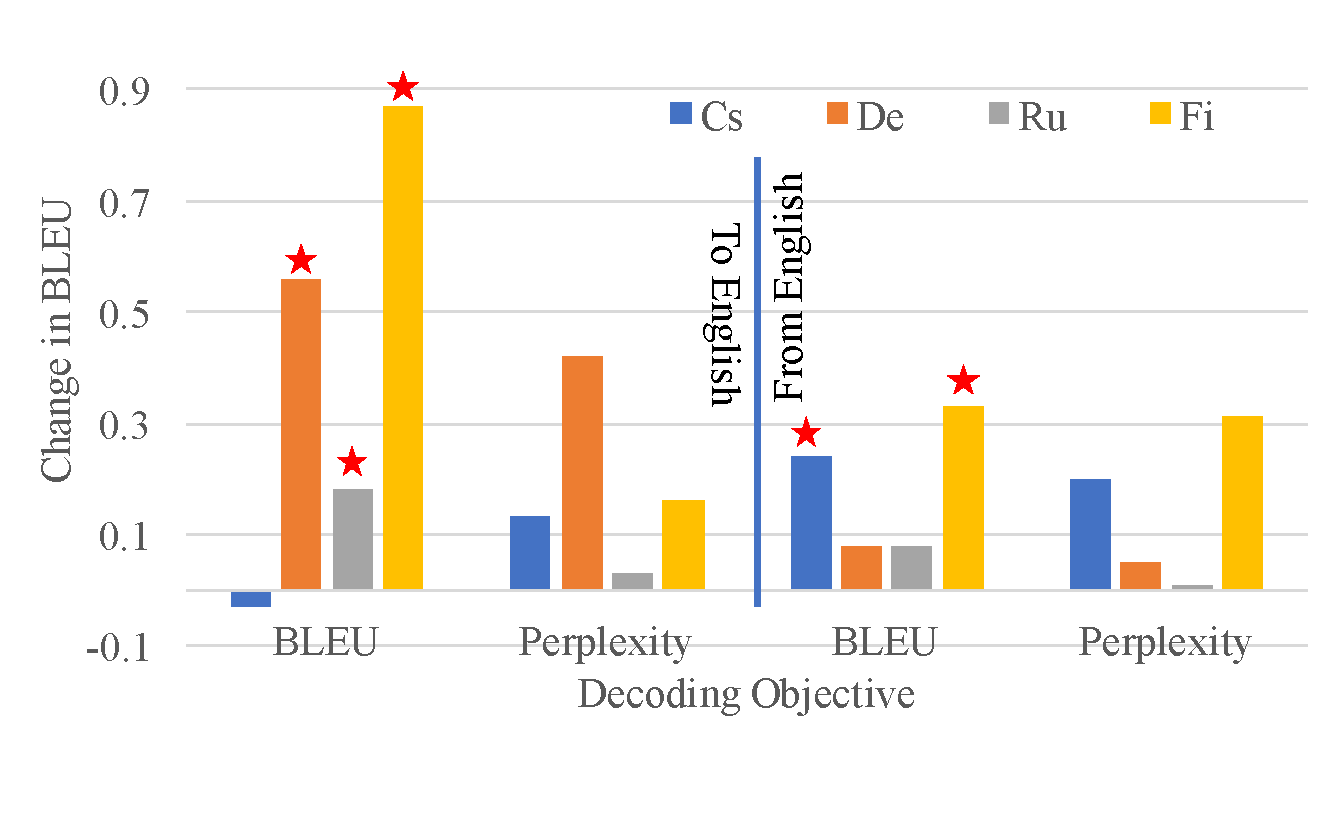
\includegraphics[width=\columnwidth]{figs/trainable/beam_bleu.pdf}
  \end{minipage}
  \hfill
  \begin{minipage}{0.48\columnwidth}
  \centering
  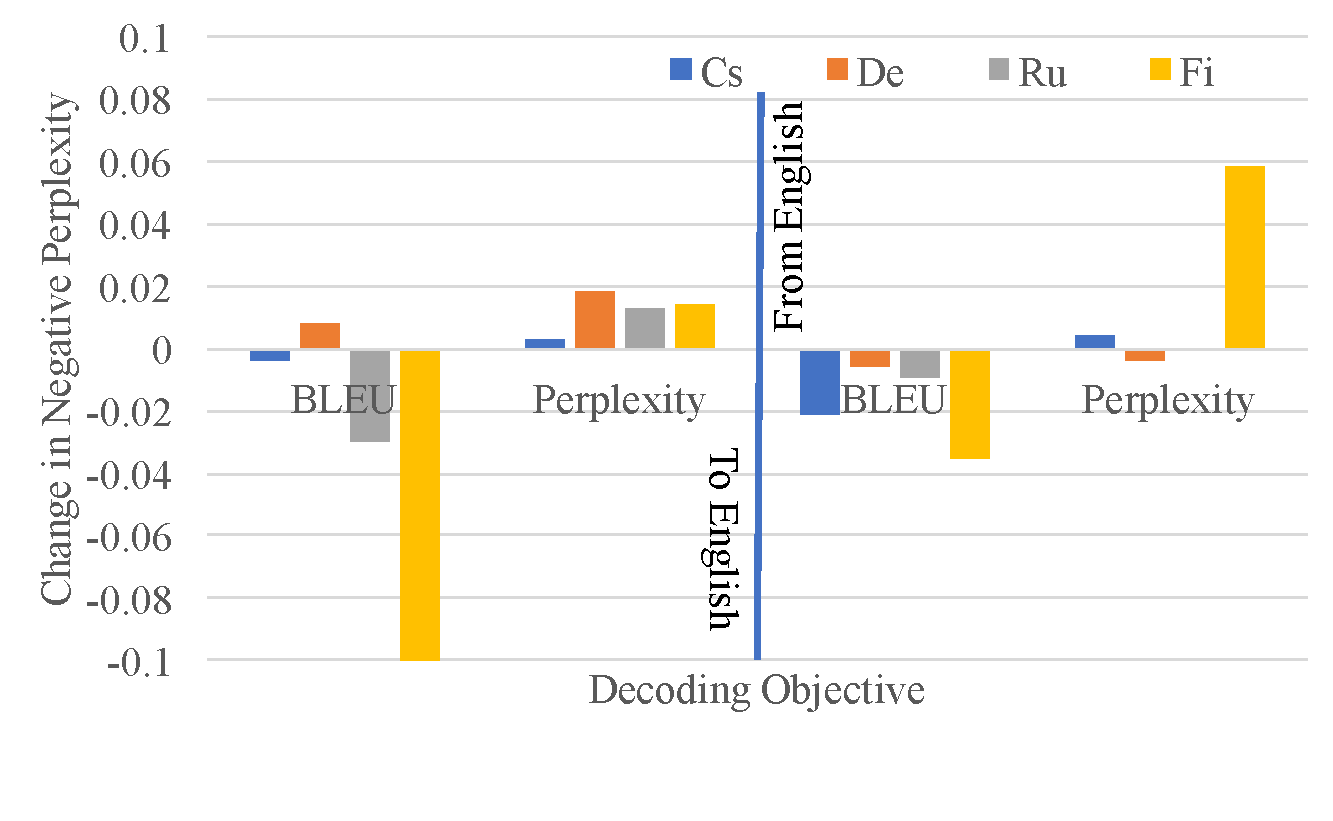
\includegraphics[width=\columnwidth]{figs/trainable/beam_perplexity.pdf}
  \end{minipage}
  \label{fig:r2}

  %\vspace{-1mm}
  (b) Beam Search + Trainable Greedy Decoding
  
  \caption{
  \label{fig:result1}
The plots draw the improvements by the trainable greedy decoding on the test set. The x-axes correspond to the objectives used to train trainable greedy decoding, and the y-axes to the changes in the achieved objectives (BLEU for the figures on the left, and negative perplexity on the right.) The top row (a) shows the cases when the trainable greedy decoder is used on its own, and the bottom row (b) when it is used together with beam search. When training and evaluation are both done with BLEU, we test the statistical significance \citep{koehn2004statistical}, and we mark significant cases with red stars ($p < 0.05$.) 
The underlying neural machine translation models achieved the BLEU scores of 14.49/16.20 for En-Cs, 18.90/21.20 for Cs-En, 18.97/21.33 for En-De, 21.63/24.46 for De-En, 16.97/19.68 for En-Ru, 21.06/23.34 for Ru-En, 7.53/8.82 for En-Fi and 9.79/11.03 for Fi-En (greedy/beam).
  }
  
\end{minipage}
% \hfill
% \begin{minipage}{0.28\textwidth}
% \caption{
% \label{fig:result1} \small
% The plots draw the improvements by the trainable greedy decoding. The x-axes correspond to the objectives used to train trainable greedy decoding, and the y-axes to the changes in the achieved objectives (BLEU for the figures on the left, and negative perplexity on the right.) The top row (a) shows the cases when the trainable greedy decoder is used on its own, and the bottom row (b) when it is used together with beam search. The baselines (improvement of 0) are respectively greedy decoding and beam search for the top and bottom rows. When training and evaluation are both done with BLEU, we test the statistical significance \citep{koehn2004statistical}, and we mark significant cases with red stars ($p < 0.05$.) 
% }
% \end{minipage}
\end{figure*}


\subsection{Critic-Aware Actor Learning}

\paragraph{Challenges}

The most apparent challenge for training such a deterministic actor with a large action space is that most of action configurations will lead to zero return. It is also not trivial to devise an efficient exploration strategy with a deterministic actor with real-valued actions. This issue has however turned out to be less of a problem than in a usual reinforcement learning setting, as the state and action spaces are well structured thanks to pretraining by maximum likelihood learning. As observed by \citet{cho2016noisy}, any reasonable perturbation to the hidden state of the recurrent network generates a reasonable translation which would receive again a reasonable return. 

Although this property of dense reward makes the problem of trainable greedy decoding more manageable, we have observed other issues during our preliminary experiment with the vanilla deterministic policy gradient. In order to avoid these issues that caused instability, we propose the following modifications to the vanilla algorithm.

% \label{sec.stabilize}
% When applying the proposed trainable decoding algorithm into practice, there is one notable property. That is, the action space is unprecedentedly high-dimensional, as the proposed actions are additive to the hidden states. Most of NMT models often have a 1000s, if not 10s of 1000s, dimensional hidden units in the decoder, making it an extremely challenging reinforcement learning problem. 
% This problem is however lessened significantly in our settings as the maximum likelihood training shapes a well-structured space for the decoder's hidden states and the actor exploits the hidden states by injecting actions on them. This constrains the exploration, the biggest challenge of learning in high-dimensional continuous space, substantially easier.

% In addition, we also proposed several methods to further stabilize the learning procedure.

%\vspace{-1mm}
\paragraph{Critic-Aware Actor Learning}
A major goal of the critic is not to estimate the return of a given episode, but to estimate the gradient of the return evaluated given an episode. In order to do so, the critic must be trained, or presented, with state-action sequences $z_{1:T'}$ similar though not identical to the state-action sequence generated by the current actor $\pi$. This is achieved, in our case, by injecting unstructured noise to the action at each time step, similar to \citep{heess2015learning}:
\begin{align}
%\vspace{-5pt}
\label{eq:noisy_actor}
\tilde{a}_t = \phi(z_t, a_{t-1}) + \sigma \cdot \epsilon,
\end{align}
where $\epsilon$ is a zero-mean, unit-variance normal variable. This noise injection procedure is mainly used when training the critic. 

We have however observed that the quality of the reward and its gradient estimate of the critic is very noisy even when the critic was trained with this kind of noisy actor. This imperfection of the critic often led to the instability in training the actor in our preliminary experiments. In order to avoid this, we describe here a technique which we refer to as {\it critic-aware actor gradient estimation}.

Instead of using the point estimate $\frac{\partial R^c}{\partial \phi}$ of the gradient of the predicted objective with respect to the actor's parameters $\phi$, we propose to use the expected gradient of the predicted objective with respect to the critic-aware distribution $Q$. That is,
\begin{align}
\label{eq:critic-aware}
\mathbb{E}_{Q}\left[\frac{\partial R^c_{\psi}}{\partial \phi}\right],
\end{align}
where we define the critic-aware distribution $Q$ as 
\begin{align}
\label{eq:critic-aware-Q}
    Q(\epsilon) \propto \exp(\underbrace{
    -(R^c_{\psi} - R)^2/\tau}_{\text{Critic-awareness}}
    )\exp(\underbrace{-\frac{\epsilon^2}{2\sigma^2}}_{\mathclap{\text{Locality}}}).
\end{align}
This expectation allows us to incorporate the noisy, non-uniform nature of the critic's approximation of the objective by up-weighting the gradient computed at a point with a higher critic quality and down-weighting the gradient computed at a point with a lower critic quality. The first term in $Q$ reflects this, while the second term ensures that our estimation is based on a small region around the state-action sequence generated by the current, noise-free actor $\pi$. 

Since it is intractable to compute Eq.~\eqref{eq:critic-aware} exactly, we resort to importance sampling with the proposed distribution equal to the second term in Eq.~\eqref{eq:critic-aware-Q}. Then, our gradient estimate for the actor becomes the sum of the gradients from multiple realizations of the noisy actor in Eq.~\eqref{eq:noisy_actor}, where each gradient is weighted by the quality of the critic $\exp(-(R^c_{\phi} - R)^2 /\tau)$. $\tau$ is a hyperparameter that controls the smoothness of the weights. We observed in our preliminary experiment that the use of this critic-aware actor learning significantly stabilizes general learning of both the actor and critic.






% \paragraph{A Noisy Actor} To encourage the exploration of the learning, a Gaussian noisy actor is used with reparameterization similar to~\newcite{heess2015learning}:
% \begin{equation}
% \label{eq.noisy_actor}
% \tilde{a}_t = a_t + \epsilon_t = \phi(z_t, a_{t-1}) + \sigma \cdot \xi_t
% \end{equation}
% where $\xi_t$ is the unit Gaussian noise. In our implementation, a small constant variance $\sigma^2$ works well for both training the critic and the actor. Note that, noise is only added in the training phase.

% \paragraph{Critic-Aware local Exploration}
% In preliminary results, we observed an instability of the approximation of true reward by the critic, which is dangerous as errors in the critic will back-propagates into the actor by Eq.~\ref{eq.chain}. On the other hand, the training of the critic also relies on the actions of the actor which potentially creates a dangerous loop when the actor fails, the critic gets worse.

% To alleviate this issue, we investigate an explicit, local exploration idea when updating the actor. Instead of adding an Gaussian noise as suggested in Eq.~\ref{eq.noisy_actor}, we includes the ``critic-awareness'' into the noise distribution $Q$, that is
% \begin{equation}
% \label{eq.critic_noise}
%     Q(\epsilon) \propto \exp(\underbrace{
%     -(R^c_{\psi} - R)^2/\tau}_{\text{Critic-awareness}}
%     )\exp(\underbrace{-\frac{\epsilon^2}{2\sigma^2}}_{\mathclap{\text{Locality}}})
% \end{equation}
% where $\tau$ is the temperature to control smoothness.
% This enables the actor to explore only the configuration in which the critic well approximates the true reward. In practice, we use importance sampling to approximately compute the gradient as
% \begin{equation}
% \label{eq.is}
% \mathbb{E}_{Q}\left[\frac{\partial R^c_{\psi}}{\partial \phi}\right] = \mathbb{E}_{N}\left[\frac{Q(\epsilon)}{N(\epsilon)} \frac{\partial R^c_{\psi}}{\partial \phi}\right] 
% \end{equation}
% where $N(\epsilon)=\mathcal{N}(0, \sigma^2)$ is the Gaussian noise. It is equivalent to reweighting the per-sample gradient using $\exp(-(R^c_{\psi} - R)^2/\tau)$.

\paragraph{Reference Translations for Training the Critic}~
In our setting of neural machine translation, we have access to a reference translation for each source sentence $X$, unlike in a usual setting of reinforcement learning. By force-feeding the reference translation into the underlying neural machine translation system (rather than feeding the decoded symbols), we can generate the reference state-action sequence. This sequence is much less correlated with those sequences generated by the actor, and facilitates computing a better estimate of the gradient w.r.t. the critic. 

%\paragraph{Break the Dependency} To avoid both the critic and the actor crash into a dangerous loop, it helps to keep the correct direction of the critic by providing the ground-truth trajectories to train the critic, or so-called \textit{teacher forcing}. More precisely, we directly feed the ground-truth $\hat{Y}$ into $\theta$ and generate a teacher sequence of hidden states $\hat{z}_{1:T}$. 

%\todo{this should go into the experimental details: Moreover, we shuffle the training set twice for separately training the critic and the actor. In this way, we can disconnect the dependency between consecutive updates and avoid a potential loop.}




% \paragraph{Train \bm{$\psi$} More} 

% As suggested in Section~\ref{sec.learn}, the critic is recommended to be sufficiently trained after each updates of the actor. %so that the critic can reasonably compute the gradient w.r.t. the actor in order to improve the true reward. 
% More precisely, we alternate training the critic and the actor with $N_c$ and $N_a$ steps respectively and keep $N_c > N_a$. 
 
In Alg.~\ref{algo2}, we present the complete algorithm. To make the description less cluttered, we only show the version of minibatch size = 1 which can be naturally extended. We also illustrate the proposed trainable greedy decoding and the proposed learning strategy in Fig.~\ref{fig:tgd}.


\section{Experimental Settings}

\begin{figure}[t]
\centering
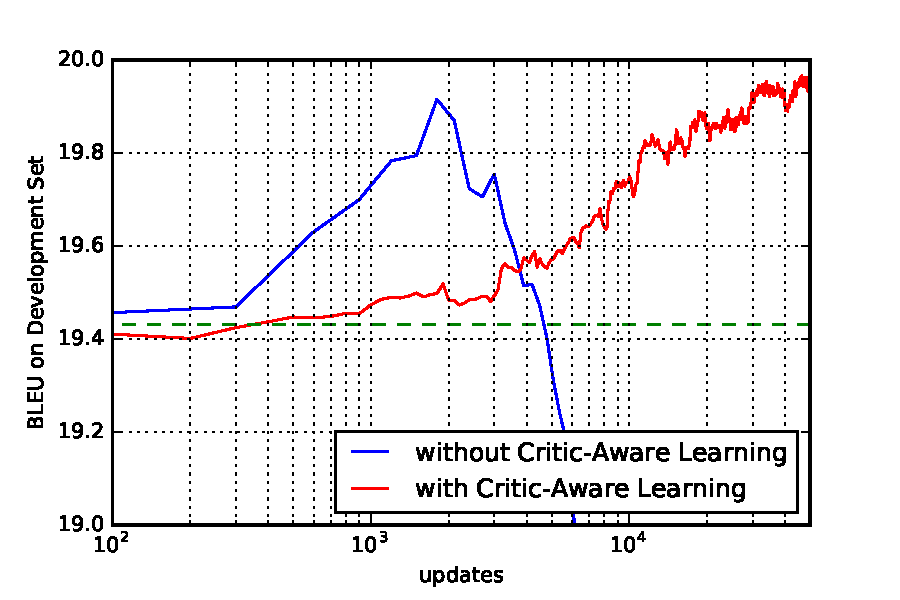
\includegraphics[width=\linewidth]{figs/trainable/lr_curve.pdf}
\vspace{-4mm}
\caption{\label{fig:lr}  
Comparison of greedy BLEU scores whether using the critic-aware exploration or not on Ru-En Dataset. The green line means the BLEU score achieved by greedy decoding from the underlying NMT model.} %{\color{red} \bf KC: Jiatao, replace the y-axis label with "BLEU on Development Set"}}
\vspace{-1mm}
\end{figure}


We empirically evaluate the proposed trainable greedy decoding on four language pairs -- En-De, En-Ru, En-Cs and En-Fi -- using a standard attention-based neural machine translation system \citep{bahdanau2014neural}. We train underlying neural translation systems using the parallel corpora made available from WMT'15.\footnote{http://www.statmt.org/wmt15/} The same set of corpora are used for trainable greedy decoding as well. All the corpora are tokenized and segmented into subword symbols using byte-pair encoding (BPE) \citep{sennrich2015neural}. We use sentences of length up to 50 subword symbols for MLE training and 200 symbols for trainable decoding. For validation and testing, we use newstest-2013 and newstest-2015, respectively.

\begin{figure*}[t]
\centering
\begin{minipage}{\textwidth}
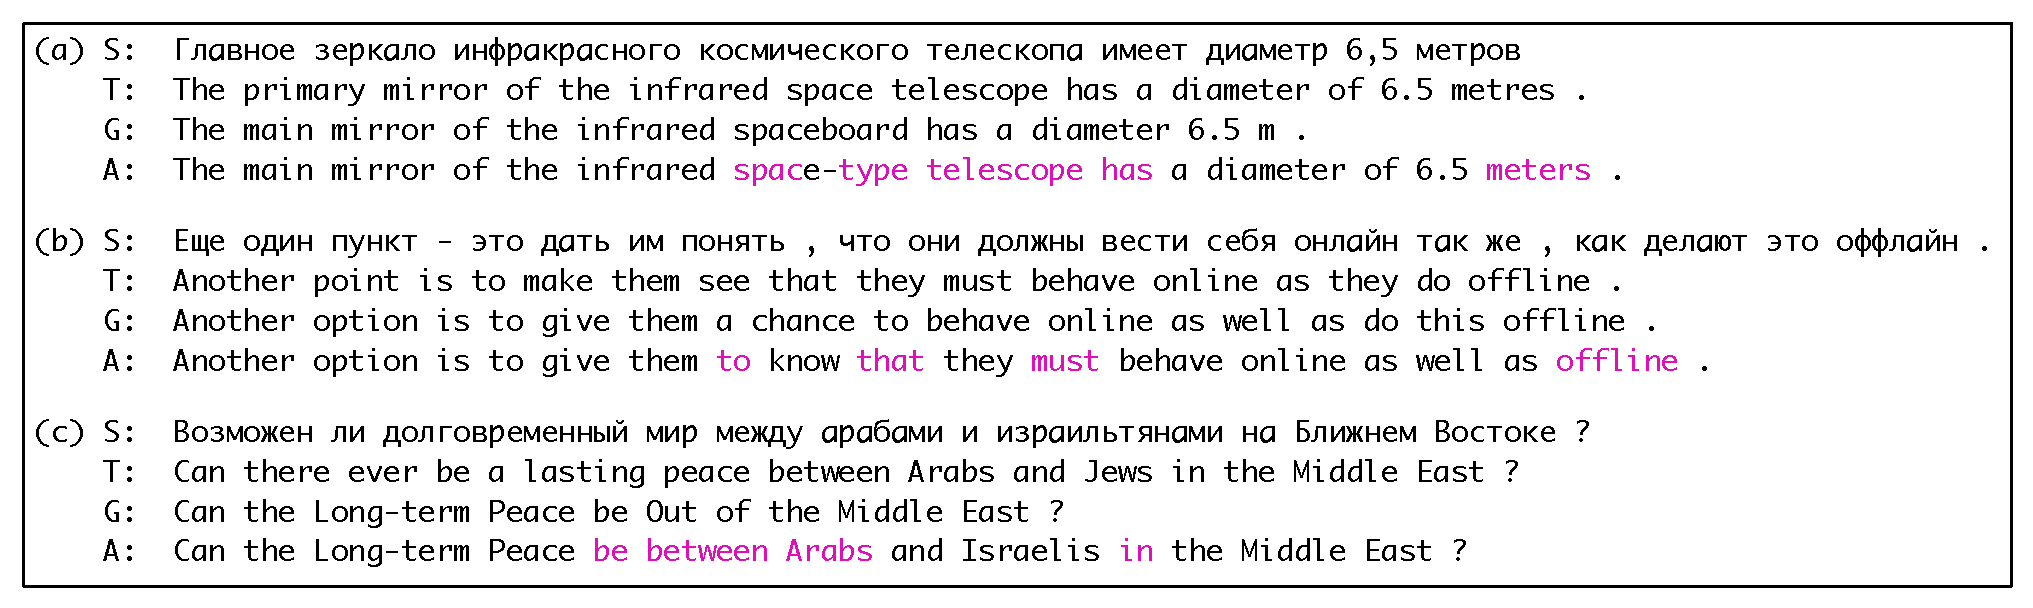
\includegraphics[width=\columnwidth]{figs/trainable/example.pdf}
\vspace{-5mm}
\caption{\label{fig:exp}   Three Ru-En examples in which the difference between the trainable greedy decoding (A) and the conventional greedy decoding (G) is large. Each step is marked with magenta, when the actor significantly influenced the output distribution.} 
\end{minipage}
% \hfill
% \begin{minipage}{0.19\textwidth}
% \caption{\label{fig:exp}  \small Three Ru-En examples in which the difference between the trainable greedy decoding (A) and the conventional greedy decoding (G) is large. Each step is marked with magenta, when the actor significantly influenced the output distribution.} 
% \end{minipage}
\vspace{-2mm}
\end{figure*}

%\vspace{-5pt}

\subsection{Model Architectures and Learning}
\paragraph{Underlying NMT Model} 
For each language pair, we implement an attention-based neural machine translation model whose encoder and decoder recurrent networks have 1,028 gated recurrent units \citep[GRU,][]{cho2014learning} each. Source and target symbols are projected into 512-dimensional embedding vectors. We trained each model for approximately 1.5 weeks using Adadelta~\citep{zeiler2012adadelta}.

%\vspace{-5pt}
\paragraph{Actor $\pi$}
We use a feedforward network with a single hidden layer as the actor. The input is a 2,056-dimensional vector which is the concatenation of the decoder hidden state and the time-dependent context vector from the attention mechanism, and it outputs a 1,028-dimensional action vector for the decoder. We use 32 units for the hidden layer with $\tanh$ activations.
%\todo{what kind of activation function? A: with tanh activation} 
 
%\vspace{-5pt}
\paragraph{Critic $R^c$}

The critic is implemented as a variant of an attention-based neural machine translation model that takes a reference translation as a source sentence and a state-action sequence from the actor as a target sentence. Both the size of GRU units and embedding vectors are the same with the underlying model.  Unlike a usual neural machine translation system, the critic does not language-model the target sentence but simply outputs a scalar value to predict the true return. When we predict a bounded return, such as sentence BLEU, we use a sigmoid activation at the output. For other unbounded return like perplexity, we use a linear activation.
%\todo{what's the size of each critic? The critic has the same with the underlying model}
%\vspace{-5pt}
\paragraph{Learning}

We train the actor and critic simultaneously by alternating between updating the actor and critic. As the quality of the critic's approximation of the decoding objective has direct influence on the actor's learning, we make ten updates to the critic before each time we update the actor once. We use RMSProp~\citep{tieleman2012lecture} with the initial learning rates of $2\times 10^{-6}$ and $2\times 10^{-4}$, respectively, for the actor and critic. 

We monitor the progress of learning by measuring the decoding objective on the validation set. After training, we pick the actor that results in the best decoding objective on the validation set, and test it on the test set.



\paragraph{Decoding Objectives}

For each neural machine translation model, pretrained using maximum likelihood criterion, we train two trainable greedy decoding actors. One actor is trained to maximize BLEU (or its smoothed version for sentence-level scoring \citep{lin2004automatic}) as its decoding objective, and the other to minimize perplexity (or equivalently the negative log-probability normalized by the length.) %\todo{are we running experiments for this? A: yes, the experiments also finished.} 
%In addition to these two, we run a limited set of experiments in which the decoding objective includes a target translation length as well as the translation quality.

We have chosen the first two decoding objectives for two purposes. First, we demonstrate that it is possible to build multiple trainable decoders with a single underlying model trained using maximum likelihood learning. Second, the comparison between these two objectives provides a glimpse into the relationship between BLEU (the most widely used automatic metric for evaluating translation systems) and log-likelihood (the most widely used learning criterion for neural machine translation).% \todo{remove if no experiment of length control} 
%The last objective is included as an example of an arbitrary objective other than translation quality.
%\vspace{-5pt}
\paragraph{Evaluation}
We test the trainable greedy decoder with both greedy decoding and beam search. Although our decoder is always trained with greedy decoding, beam search in practice can be used together with the actor of the trainable greedy decoder. Beam search is expected to work better especially when our training of the trainable greedy decoder is unlikely to be optimal. In both cases, we report both the perplexity and BLEU.


\subsection{Results and Analysis}

We present the improvements of BLEU and perplexity (or its negation) in Fig.~\ref{fig:result1} for all the language pair-directions. It is clear from these plots that the best result is achieved when the trainable greedy decoder was trained to maximize the target decoding objective. When the decoder was trained to maximize sentence-level BLEU, we see the improvement in BLEU but often the degradation in the perplexity (see the left plots in Fig.~\ref{fig:result1}.) On the other hand, when the actor was trained to minimize the perplexity, we only see the improvement in perplexity (see the right plots in Fig.~\ref{fig:result1}.) This confirms our earlier claim that it is necessary and desirable to tune for the target decoding objective regardless of what the underlying translation system was trained for, and strongly supports the proposed idea of trainable decoding.

The improvement from using the proposed trainable greedy decoding is smaller when used together with beam search, as seen in Fig.~\ref{fig:result1}~(b). However, we still observe statistically significant improvement in terms of BLEU (marked with red stars.) This suggests a future direction in which we extend the proposed trainable greedy decoding to directly incorporate beam search into its training procedure to further improve the translation quality. 

It is worthwhile to note that we achieved all of these improvements with negligible computational overhead. This is due to the fact that our actor is a very small, shallow neural network, and that the more complicated critic is thrown away after training. We suspect the effectiveness of such a small actor is due to the well-structured hidden state space of the underlying neural machine translation model which was trained with a large amount of parallel corpus. We believe this favourable computational complexity makes the proposed method suitable for production-grade neural machine translation \citep{wu2016google,crego2016systran}.



% \paragraph{BLEU v.s. Perplexity} 
% As shown in Fig.~\ref{fig:result1}, When using sentence BLEU as objectives, most of the language pairs achieve improvements on both BLEU scores but have a large drop on perplexity. In contrast, most of the language pairs still get improvements on BLEU scores (not as good as directly optimizing the BLEU scores) when using perplexity as the decoding objectives.% which may indicate that the proposed trainable decoding algorithms works more effective when using the BLEU score as the target. 
% Although there is a strong connection between improving BLEU scores and perplexity, since the model we used to compute the perplexity is commonly imperfect to recover the true distribution, there maybe a mismatch between when directly optimizing the BLEU scores.

% \paragraph{Greedy v.s. Beam search}
% Overall, the improvement of doing beam search is relatively smaller than evaluating with greedy decoding for all the language pairs and objectives, which is natural as the proposed algorithm optimizes only when doing greedy decoding. Moreover, by comparing the Fig.~\ref{fig:result1} (a) and (b) pair by pair, we can also find a clear correlation of the improvements between greedy decoding and beam search, especially for pairs with English on the target side. It suggests that once the decoder is optimized with trainable greedy decoding, we can do beam search better.

% \paragraph{Significance Analysis}
% We can also find that not all the language pairs can achieve a significant improvement at similar levels with the trainable decoding. For example, when using BLEU score as the objective, all the pairs with English as source language can have a significant improvement, while on the reverse direction, the improvement of Cs-En and Ru-En are quite small (or even negative). Similarly, when using perplexity as decoding objectives, the model of En-Fi works much worse than the underlying model. Although the majority of the results show the effectiveness of the proposed trainable decoding algorithm, we still need to tune and be careful when using it for specific situations.

\paragraph{Importance of Critic-Aware Actor Learning}
In Fig.~\ref{fig:lr}, we show sample learning curves with and without the proposed critic-aware actor learning. Both curves were from the models trained under the same condition. Despite a slower start in the early stage of learning, we see that the critic-aware actor learning has greatly stabilized the learning progress. We emphasize that we would not have been able to train all these 16 actors without the proposed critic-aware actor learning.

\paragraph{Examples} 
In Fig.~\ref{fig:exp}, we present three examples from Ru-En. We defined the influence as the KL divergence between the conditional distributions without the trainable greedy decoding and with the trainable greedy decoding, assuming the fixed previous hidden state and target symbol. We colored a target word with magenta, when the influence of the trainable greedy decoding is large ($> 0.001$).  Manual inspection of these examples as well as others has revealed that the trainable greedy decoder focuses on fixing prepositions and removing any unnecessary symbol generation. More in-depth analysis is however left as future work. 

\section{Conclusion}

We proposed trainable greedy decoding as a way to learn a decoding algorithm for neural machine translation with an arbitrary decoding objective. The proposed trainable greedy decoder observes and manipulates the hidden state of a trained neural translation system, and is trained by a novel variant of deterministic policy gradient, called critic-aware actor learning. Our extensive experiments on eight language pair-directions and two objectives confirmed its validity and usefulness. The proposed trainable greedy decoding is a generic idea that can be applied to any recurrent language modeling, and we anticipate future research both on the fundamentals of the trainable decoding as well as on the applications to more diverse tasks such as image caption generating and dialogue modeling.



\chapter{Non-Autoregressive Neural Machine Translation}
\label{nat}
\def \model{NAT}

\section{Overview}
Neural network based models outperform traditional statistical models for machine translation (MT) \citep{bahdanau2014neural,luong2015effective}. 
However, state-of-the-art neural models are much slower than statistical MT approaches at inference time \citep{wu2016google}.
Both model families use \emph{autoregressive} decoders that operate one step at a time: they generate each token conditioned on the sequence of tokens previously generated. This process is not parallelizable, and, in the case of NMT models, it is particularly slow because a computationally intensive neural network is used to generate each token.

While several recently proposed models avoid recurrence at train time by leveraging convolutions~\citep{kalchbrenner2016neural, gehring2017convolutional, kaiser2017depthwise} or self-attention (the Transformer network)~\citep{vaswani2017attention} as more-parallelizable alternatives to recurrent neural networks (RNNs), use of autoregressive decoding makes it impossible to take full advantage of parallelism during inference.

In this chapter, we introduce a non-autoregressive translation model based on the Transformer network~\citep{vaswani2017attention}. We modify the encoder of the original Transformer network by adding a module that predicts \emph{fertilities}, sequences of numbers that form an important component of many traditional machine translation models \citep{brown1993mathematics}. These fertilities are supervised during training and provide the decoder at inference time with a globally consistent plan on which to condition its simultaneously computed outputs. Through knowledge distillation, the use of fertilities as a latent variable, and policy gradient fine-tuning, we achieve this at a cost of as little as 2.0 BLEU points relative to the autoregressive Transformer network used as a teacher.
We demonstrate substantial cumulative improvements associated with each of the three aspects of our training strategy, and validate our approach on IWSLT 2016 English--German and two WMT language pairs. By sampling fertilities in parallel at inference time, our non-autoregressive model achieves near-state-of-the-art performance of 29.8 BLEU on WMT 2016 English--Romanian.

%\subsection{Autoregressive Neural Machine Translation}
%Given a source sentence $X=\{x_1, ..., x_{T'}\}$, a neural machine translation model factors the distribution over possible output sentences $Y=\{y_1, ..., y_T\}$ into a chain of conditional probabilities with a left-to-right causal structure:
%\begin{equation}
%p_{\mathcal{AR}}(Y|X; \theta) = \prod_{t=1}^{T+1} p(y_t| y_{0:t-1}, x_{1:T'}; \theta),
%\end{equation}
%where the special tokens $y_0$ (e.g. $\langle \mathrm{bos}\rangle$) and $y_{T+1}$ (e.g. $\langle \mathrm{eos}\rangle$) are used to represent the beginning and end of all target sentences.
%These conditional probabilities are parameterized using a neural network. Typically, an encoder-decoder architecture~\citep{sutskever2014sequence} with a unidirectional RNN-based decoder is used to capture the causal structure of the output distribution.
%
%\vspace{-5pt}
%\paragraph{Maximum Likelihood training}
%Choosing to factorize the machine translation output distribution autoregressively enables straightforward maximum likelihood training with a cross-entropy loss applied at each decoding step:
%\begin{equation}
%\mathcal{L}_{\text{ML}} = \log p_{\mathcal{AR}}(Y|X; \theta) = \sum_{t=1}^{T+1}\log p(y_t|y_{0:t-1},x_{1:T'};\theta).
%\end{equation}
%This loss provides direct supervision for each conditional probability prediction.
%
%\vspace{-5pt}
%\paragraph{Autoregressive NMT without RNNs}
%Since the entire target translation is known at training time, the calculation of later conditional probabilities (and their corresponding losses) does not depend on the output words chosen during earlier decoding steps. Even though decoding must remain entirely sequential during inference, models can take advantage of this parallelism during training.
%One such approach replaces recurrent layers in the decoder with masked convolution layers~\citep{kalchbrenner2016neural, gehring2017convolutional} that provide the causal structure required by the autoregressive factorization.
%
%A recently introduced option which reduces sequential computation still further is to construct the decoder layers out of self-attention computations that have been causally masked in an analogous way.
%The state-of-the-art Transformer network takes this approach, which allows information to flow in the decoder across arbitrarily long distances in a constant number of operations, asymptotically fewer than required by convolutional architectures \citep{vaswani2017attention}.

\begin{figure}[t]
\centering
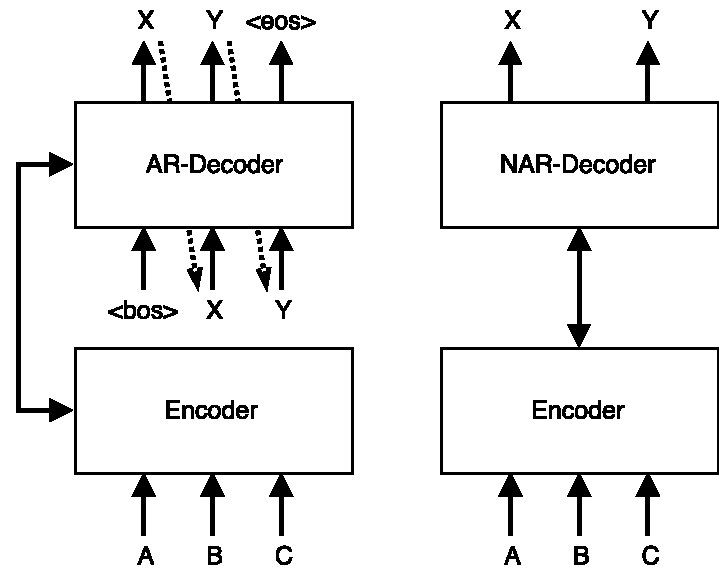
\includegraphics[width=0.6\linewidth]{figs/nat/ar_nmt}
\caption{\label{cp8.fig.ar_vs_nar} Translating ``A B C'' to ``X Y'' using autoregressive and non-autoregressive neural MT architectures. The latter generates all output tokens in parallel.}
\end{figure}


\section{Non-Autoregressive Decoding}
\paragraph{Pros and cons of autoregressive decoding}
The autoregressive factorization (i.e. Eq.~\eqref{cp2.eq.auto_sts}, see details in Chapter~\ref{background}) used by conventional NMT models has several benefits. It corresponds to the word-by-word nature of human language production and effectively captures the distribution of real translations. Autoregressive models achieve state-of-the-art performance on large-scale corpora and are easy to train, while beam search provides an effective local search method for finding approximately-optimal output translations.

But there are also drawbacks. As the individual steps of the decoder must be run sequentially rather than in parallel, autoregressive decoding prevents architectures like the Transformer from fully realizing their train-time performance advantage during inference. Meanwhile, beam search suffers from diminishing returns with respect to beam size \citep{koehn2017six} and exhibits limited search parallelism because it introduces computational dependence between beams.


\paragraph{Towards non-autoregressive decoding}
A na\"{i}ve solution is to remove the autoregressive connection directly from an existing encoder-decoder model. Assuming that the target sequence length $T$ can be modeled with a separate conditional distribution $p_L$, this becomes
\begin{equation}
p_{\mathcal{NA}}(Y|X; \theta) = p_L(T|x_{1:T'};\theta)\cdot \prod_{t=1}^T p(y_t| x_{1:T'};\theta).
\label{eq.simple}
\end{equation}
This model still has an explicit likelihood function, and it can still be trained using independent cross-entropy losses on each output distribution. Now, however, these distributions can be computed in parallel at inference time. 

\subsection{The Multimodality Problem}
However, this na\"{i}ve approach does not yield good results, because such a model exhibits complete \emph{conditional independence}.
Each token's distribution $p(y_t)$  depends only on the source sentence $X$. 
This makes it a poor approximation to the true target distribution, which exhibits strong correlation across time. 
Intuitively, such a decoder is akin to a panel of human translators each asked to provide a single word of a translation independently of the words their colleagues choose.

In particular, consider an English source sentence like ``Thank you.'' This can be accurately translated into German as any one of ``Danke.'', ``Danke sch\"{o}n.'', or ``Vielen Dank.'', all of which may occur in a given training corpus. This target distribution cannot be represented as a product of independent probability distributions for each of the first, second, and third words, because a conditionally independent distribution cannot allow ``Danke sch\"{o}n.'' and ``Vielen Dank.'' without also licensing ``Danke Dank.'' and ``Vielen sch\"{o}n.''

The conditional independence assumption prevents a model from properly capturing the highly multimodal distribution of target translations.
We call this the ``multimodality problem'' and introduce both a modified model and new training techniques to tackle this issue.

\section{The Non-Autoregressive Transformer (NAT)}
\label{cp8.sec.mainModelSection}

In this section, we introduce a novel NMT model---the Non-Autoregressive Transformer (\model)---that can produce an entire output translation in parallel.
As shown in Fig.~\ref{cp8.fig.diagram}, the model is composed of the following four modules: 
an encoder stack, 
a decoder stack, 
a newly added fertility predictor (details in \ref{cp8.sec.fertility}), and a translation predictor for token decoding. 

\begin{figure}[t]
\centering
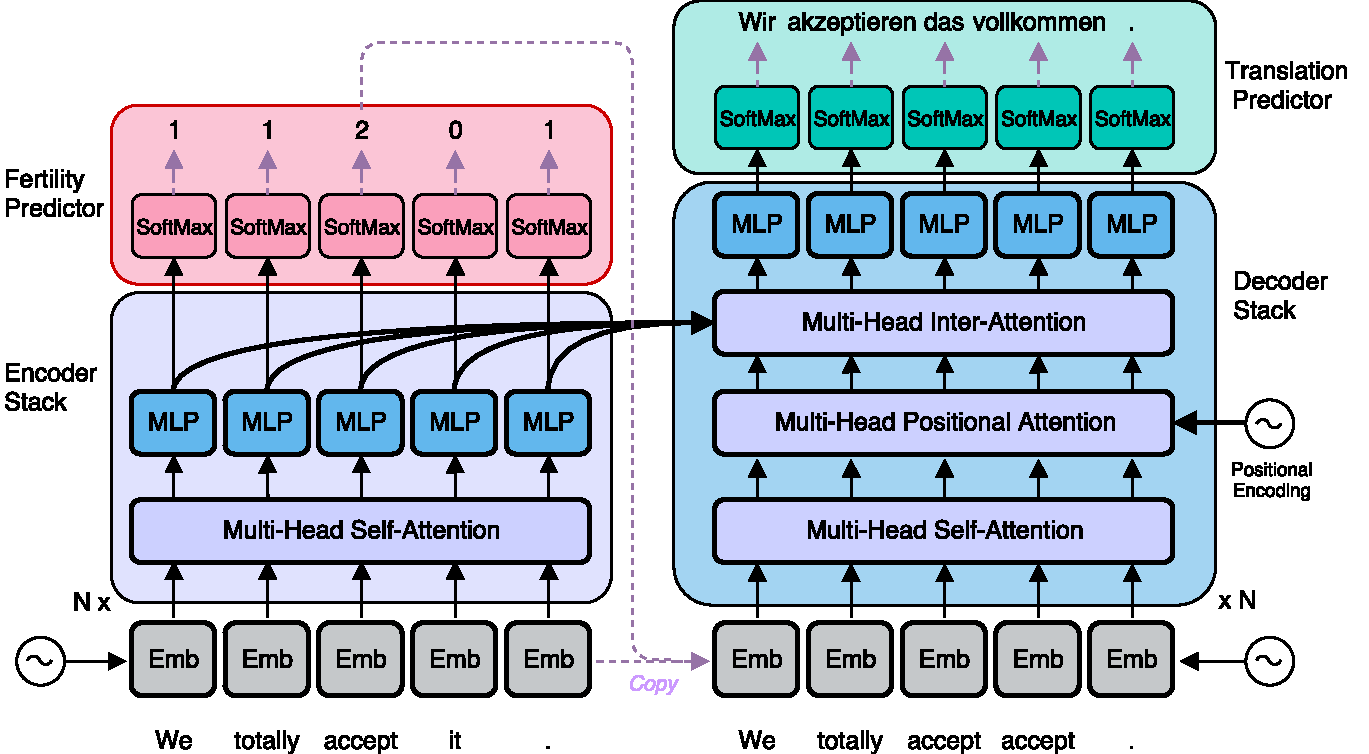
\includegraphics[width=\textwidth]{figs/nat/NAT-sub}
\caption{\label{cp8.fig.diagram} The architecture of the \model{}, where the black solid arrows represent differentiable connections and the purple dashed arrows are non-differentiable operations. Each sublayer inside the encoder and decoder stacks also includes layer normalization and a residual connection.}
\end{figure}

\subsection{Encoder Stack}
Similar to the autoregressive Transformer, both the encoder and decoder stacks are composed entirely of feed-forward networks (MLPs) and multi-head attention modules. Since no RNNs are used, there is no inherent requirement for sequential execution, making non-autoregressive decoding possible.
% Each attention operation takes the query (Q), key (K) and value (V) as inputs:
% \begin{equation}
% \text{Attention}(Q,K,V)=\text{softmax}\left(\frac{QK^T}{\sqrt{d_{\text{model}}}}\right)\cdot V
% \label{cp8.eq.attention}
% \end{equation}
% where $d_{\text{model}}$ is the model hidden size.
For our proposed \model{}, the encoder stays unchanged from the original Transformer network.

\subsection{Decoder Stack}\label{cp8.sec.decoderStack}
In order to translate non-autoregressively and parallelize the decoding process, we modify the decoder stack as follows.

\paragraph{Decoder Inputs}
Before decoding starts, the \model{} needs to know how long the target sentence will be in order to generate all words in parallel.
More crucially, we cannot use time-shifted target outputs (during training) or previously predicted outputs (during inference) as the inputs to the first decoder layer.
Omitting inputs to the first decoder layer entirely, or using only positional embeddings, resulted in very poor performance.
Instead, we initialize the decoding process using copied source inputs from the encoder side. As the source and target sentences are often of different lengths, we propose two methods:
\begin{itemize}
\item \textbf{Copy source inputs uniformly}: Each decoder input $t$ is a copy of the $\textrm{Round}(T'\cdot t/T)$-th encoder input. This is equivalent to ``scanning'' source inputs from left to right with a constant ``speed,'' and results in a decoding process that is deterministic given a (predicted) target length.
\item \textbf{Copy source inputs using fertilities}: A more powerful way, depicted in Fig.~\ref{cp8.fig.diagram} and discussed in more detail below, 
is to copy each encoder input as a decoder input zero or more times, with the number of times each input is copied referred to as that input word's ``fertility.''
% is to copy the position of $\arg\min_{k}{\sum_{t'=1}^{k}}f_{t'}\geq t$ for each position $t$ where for each source word $x_{t'}$, a special \textit{fertility} score $f_{t'} (\geq 0)$ is predicted.
In this case the source inputs are scanned from left to right at a ``speed'' that varies inversely with the fertility of each input; the decoding process is now conditioned on the sequence of fertilities, while the resulting output length is determined by the sum of all fertility values. 
\end{itemize}


\paragraph{Non-causal self-attention}
Without the constraint of an autoregressive factorization of the output distribution, we no longer need to prevent earlier decoding steps from accessing information from later steps. Thus we can avoid the causal mask used in the self-attention module of the conventional Transformer's decoder. Instead, we  mask out each query position only from attending to itself, which we found to improve decoder performance relative to unmasked self-attention.


\paragraph{Positional attention}
We also include an additional positional attention module in each decoder layer, which is a multi-head attention module with the same general attention mechanism used in other parts of the Transformer network, i.e.
\begin{equation}
\text{Attention}(Q,K,V)=\text{softmax}\left(\frac{QK^T}{\sqrt{d_\text{model}}}\right)\cdot V,
\label{cp8.eq.attention}
\end{equation}
where $d_\text{model}$ is the model hidden size, but with the positional encoding\footnote{The positional encoding $p$ is computed as $p(j, k) =
\sin{(j/10000^{k/d})}$ (for even $k$) or $\cos{(j/10000^{k/d})}$ (for odd $k$), where $j$ is the timestep index and $k$ is the channel index.} as both query ($Q$) and key ($K$) and the decoder states as the value ($V$). This incorporates positional information directly into the attention process and provides a stronger positional signal than the embedding layer alone. We also hypothesize that this additional information improves the decoder's ability to perform local reordering. More details and discussion about this style of multi-head attention can be found in \cite{vaswani2017attention}.

\subsection{Modeling Fertility to Tackle the Multimodality Problem}
\label{cp8.sec.fertility}

\paragraph{Latent Variable Model}
The multimodality problem can be attacked by introducing a latent variable $\zeta$ to directly model the nondeterminism in the translation process: we first sample $\zeta$ from a prior distribution and then condition on $\zeta$ to non-autoregressively generate a translation. That is:
 \begin{equation}
 \label{cp8.eq.latent}
 p_{\mathcal{NA}}(Y|X; \theta) = \sum_\zeta{\left[p_\zeta(\zeta|x_{1:T'};\theta)\cdot p_L(T|x_{1:T'};\theta;\zeta)\cdot \prod_{t=1}^T p(y_t| x_{1:T'};\theta;\zeta)\right]},
 \end{equation}
 where one way to interpret this latent variable $\zeta$  is as a sentence-level ``plan'' akin to those discussed in the language production literature~\citep{martin2010planning}. There are several desirable properties for this latent variable:
\begin{itemize}
\item It should be simple to infer a value for the latent variable given a particular input-output pair, as this is needed to train the model end-to-end.
\item Adding $\zeta$ to the conditioning context should account as much as possible for the correlations across time between different outputs, so that the remaining marginal probabilities at each output location are as close as possible to satisfying conditional independence.
\item It should not account for the variation in output translations so directly that $p(y|x, \zeta)$ becomes trivial to learn, since that is the function our decoder neural network will approximate.
\end{itemize}
The factorization by length introduced in Eq.~\eqref{eq.simple} provides a very weak example of a latent variable model, satisfying the first and third property but not the first. We propose the use of \emph{fertilities} instead. These are integers for each word in the source sentence that correspond to the number of words in the target sentence that can be aligned to that source word using a hard alignment algorithm like IBM Model 2 \citep{brown1993mathematics}\footnote{The concept of fertilities are officially introduced in IBM Model 3. However, we use a simplified version which are computed from the word-alignment used in IBM model 2.}.


\paragraph{Latent Fertility Model}
One of the most important properties of the proposed \model{} is that it naturally introduces an informative latent variable when we choose to copy the encoder inputs based on predicted fertilities.  More precisely, given a source sentence $X$, the conditional probability of a target translation $Y$ is:
\begin{equation}
p_{\mathcal{NA}}(Y|X; \theta) = \sum_{f_1,...,f_{T'} \in \mathcal{F}}\left(\prod_{t'=1}^{T'}p_F(f_{t'}|x_{1:T'};\theta)\cdot \prod_{t=1}^{T} p(y_t| x_1\{f_1\}, .., x_{T'}\{f_{T'}\};\theta)\right)
\label{cp8.eq.latent_fer}
\end{equation}
where $\mathcal{F}=\{f_1,...,f_{T'}| \sum_{t'=1}^{T'}f_{t'}= T, f_{t'} \in \mathbb{Z^*} \}$ is the set of all fertility sequences---one fertility value per source word---that sum to the length of $Y$ and $x\{f\}$ denotes the token $x$ repeated $f$ times.

\paragraph{Fertility prediction} As shown in Fig.~\ref{cp8.fig.diagram}, we model the fertility $p_F(f_{t'}|x_{1:T'})$ at each position independently using a one-layer neural network with a softmax classifier ($L=50$ in our experiments) on top of the output of the last encoder layer. This models the way that fertility values are a property of each input word but depend on information and context from the entire sentence.


\paragraph{Benefits of fertility} 
Fertilities possess all three of the properties listed earlier as desired of a latent variable for non-autoregressive machine translation:
\begin{itemize}
\item An external aligner provides a simple and fast approximate inference model that effectively reduces the unsupervised training problem to two supervised ones.
\item Using fertilities as a latent variable makes significant progress towards solving the multimodality problem by providing a natural factorization of the output space.
Given a source sentence, restricting the output distribution to those target sentences consistent with a particular fertility sequence dramatically reduces the mode space. Furthermore, the global choice of mode is factored into a set of local mode choices: namely, how to translate each input word. These local mode choices can be effectively supervised because the fertilities provide a fixed ``scaffold.''
\item Including both fertilities and reordering in the latent variable would provide complete alignment statistics. This would make the decoding function trivially easy to approximate given the latent variable and force all of the modeling complexity into the encoder. Using fertilities alone allows the decoder to take some of this burden off of the encoder.
\end{itemize}
Our use of fertilities as a latent variable also means that there is no need to have a separate means of explicitly modeling the length of the translation, which is simply the sum of fertilities.
% The sum of fertilities completely determines the length of the translation.
%Furthermore, as the fertilities are predicted locally, any mis-prediction of fertilities will not cause a dramatic change in the final length.
And fertilities provide a powerful way to condition the decoding process, allowing the model to generate diverse translations by sampling over the fertility space.

\subsection{Translation Predictor and the Decoding Process}
At inference time, the model can identify the translation with the highest conditional probability (see Eq.~\eqref{cp8.eq.latent_fer}) by marginalizing over all possible latent fertility sequences. 
Given a fertility sequence, however, identifying the optimal translation only requires independently maximizing the local probability for each output position.
% \begin{equation}
% \hat{Y} = \argmax_{Y}p_{\mathcal{NA}}(Y|X;\theta)=\argmax_{Y\in \mathcal{M}}p_{\mathcal{NA}}(Y|X;\theta),
% \end{equation}
% where $\mathcal{M}=\{\hat{y}_{1: T}|\hat{y}_t  = \argmax_{y_t} p\left(y_t|x_1\{f_1\}, .., x_{T'}\{f_{T'}\}\right);\theta), t=1, ..., T, \forall f_{1:T'}\}$.  
We define $Y = G(x_{1:T'}, f_{1:T'}; \theta)$ to represent the optimal translation given a source sentence and a sequence of fertility values.
But searching and marginalizing over the whole fertility space is still intractable. We propose three heuristic decoding algorithms to reduce the search space of the \model{} model:

\paragraph{Argmax decoding} Since the fertility sequence is also modeled with a conditionally independent factorization, we can simply estimate the best translation by choosing the highest-probability fertility for each input word:
\begin{equation}
	\hat{Y}_\text{argmax} = G(x_{1:T'}, \hat{f}_{1:T'};\theta), \textrm{where} \ \ \hat{f}_{t'}=\argmax_f p_F(f_{t'}|x_{1:T'};\theta)
\end{equation}
%When not otherwise specified, our experiments use argmax decoding.

\paragraph{Average decoding}
We can also estimate each fertility as the expectation of its corresponding softmax distribution:
\begin{equation}
	\hat{Y}_\text{average} = G(x_{1:T'}, \hat{f}_{1:T'};\theta), \textrm{where} \ \ \hat{f}_{t'}=\textrm{Round}\left(\sum_{f_{t'}=1}^L p_F(f_{t'}|x_{1:T'};\theta)f_{t'}\right)
    \label{cp8.eq.average}
\end{equation}

\paragraph{Noisy / Exact parallel decoding (NPD/EPD)} A more accurate approximation of the true optimum of the target distribution, inspired by~\citet{cho2016noisy} (which is also been discussed in \S\ref{cp2.sec.noisy}), is to draw samples from the fertility space and compute the best translation for each fertility sequence based on  a re-rank function.
% %it is possible by injecting unstructured noise to the hidden states of the NMT models and decoding in completely parallel to find the best translation. In \model{},  we can do similar noisy decoding by directly sampling in the fertility space where the best translation can be re-ranked based on the probabilities, that is:
% \begin{equation}
% \hat{Y}_\text{NPD} = G(x_{1:T'}, \argmax_{f_{t'} \sim p_F(f_{t'}|x_{1:T'})} p_{\mathcal{NA}}(G(x_{1:T'}, f_{1:T'})|X))
% \end{equation}
% \paragraph{Noisy parallel decoding with conceptual loss (NPDC)}
% The same idea of noisy decoding can also be applied with any scoring or ranking function. For instance, after obtaining the best translation for each sampled fertility sequence using our non-autoregressive model, 
We can then use the autoregressive teacher to identify the best overall translation:
%to be analogy to beam-search for autoregressive models, we can also do the same noisy parallel decoding but use the pre-trained autoregressive model to assign scores for each translation.  
\begin{equation}
\hat{Y}_\text{NPD} = G(x_{1:T'}, \argmax_{f_{t'} \sim p_F} p_{\mathcal{AR}}(G(x_{1:T'}, f_{1:T'};\theta)|X;\theta);\theta)
\end{equation}

NPD is a stochastic search method which cannot make sure to result in the same translation for each run. Also, it is likely to produce duplicated fertilities when we simply sample from the distribution. An alternative is to incorporate an ``Exact parallel decoding'' in the fertility space instead of sampling, considering its factorized formulation of the distribution of fertility. In such cases, everything will be the same except we use the searched fertilities  to compute the translation. That is:
\begin{equation}
\hat{Y}_\text{EPD} = G(x_{1:T'}, \argmax_{f_{t'}  \in \argsort^K p_F} p_{\mathcal{AR}}(G(x_{1:T'}, f_{1:T'};\theta)|X;\theta);\theta)
\end{equation}
Searching in the fertility space usually costs another $10\sim20\%$ overhead of the computational time compared to sampling, in the meantime, it generally improves the final performance by $0.5$ BLEU scores.
Also, when using an autoregressive model as a scoring function for a set of decoded translations, it can run as fast as it does at train time because it can be provided with all decoder inputs in parallel.

Both NPD and EPD also increase the computational resources required linearly by the sample size. However, because all the search samples can be computed and scored entirely independently, the process only doubles the latency compared to computing a single translation if sufficient parallelism is available.
%the latency caused by autoregressive models, all our search samples are completely independent with each other, and theoretically can be computed without any latency, which will be more applicable in industry settings.


\section{Learning}
The proposed \model{} contains a discrete sequential latent variable $f_{1:T'}$, whose conditional posterior distribution $p(f_{1:T'} | x_{1:T'}, y_{1:T}; \theta)$ we can approximate using a proposal distribution $q(f_{1:T'} | x_{1:T'}, y_{1:T})$. This provides a variational bound for the overall maximum likelihood loss:
\begin{equation}
\label{cp8.eq.variational}
\begin{split}
\mathcal{L}_{\text{ML}} &= \log p_{\mathcal{NA}}(Y|X; \theta) = \log \sum_{f_{1:T'}\in \mathcal{F}}{p_F(f_{1:T'}|x_{1:T'}; \theta)\cdot p(y_{1:T} | x_{1:T'}, f_{1:T'}; \theta)} \\
&\geq \mathop{\mathbb{E}}_{f_{1:T'} \sim q}\left(\underbrace{\sum_{t=1}^T\log p(y_t| x_1\{f_1\}, .., x_{T'}\{f_{T'}\}; \theta)}_{\text{Translation Loss}} + \underbrace{\sum_{t'=1}^{T'}\log p_F(f_{t'}|x_{1:T'}; \theta)}_{\text{Fertility Loss}} \right) + \mathcal{H}(q)
\end{split}
\end{equation}

We choose a proposal distribution $q$ defined by a separate, fixed fertility model. Possible options include the output of an external aligner, which produces a deterministic sequence of integer fertilities for each (source, target) pair in a training corpus, or fertilities computed from the attention weights used in our fixed autoregressive teacher model. This simplifies the inference process considerably, as the expectation over $q$ is deterministic.

The resulting loss function, consisting of the two bracketed terms in Eq.~\eqref{cp8.eq.variational}, allows us to train the entire model in a supervised fashion, using the inferred fertilities to simultaneously train the translation model $p$ and supervise the fertility network model $p_F$.

\subsection{Sequence-Level Knowledge Distillation}\label{cp8.sec.seqkd}

While the latent fertility model substantially improves the ability of the non-autoregressive output distribution to approximate the multimodal target distribution, it does not completely solve the problem of nondeterminism in the training data. In many cases, there are multiple correct translations consistent with a single sequence of fertilities---for instance, both ``Danke sch\"{o}n.'' and ``Vielen dank.'' are consistent with the English input ``Thank you.'' and the fertility sequence $[2, 0, 1]$, because ``you'' is not directly translated in either German sentence.

Thus we additionally apply sequence-level knowledge distillation~\citep{kim2016sequence} to construct a new corpus by training an autoregressive machine translation model, known as the teacher, on an existing training corpus, then using that model's greedy outputs as the targets for training the non-autoregressive student. The resulting targets are less noisy and more deterministic, as the trained model will consistently translate a sentence like ``Thank you.'' into the same German translation every time; on the other hand, they are also lower in quality than the original dataset.

% Training using knowledge distillation typically aims to minimize the divergence between the output distributions of a trainable student network and a fixed teacher network. Expressed at the sequence level, that means minimizing a loss like 
% \begin{equation}
% \mathcal{L}_\text{KD} = −\sum_{t\in T}{q(t | s) \log p(t | s)}
% \end{equation}
% Instead of using the real data using greedy or beam search

\subsection{Fine-Tuning}
Our supervised fertility model enables a decomposition of the overall maximum likelihood loss into translation and fertility terms, but it has some drawbacks compared to variational training.
In particular, it heavily relies on the deterministic, approximate inference model provided by the external alignment system, while it would be desirable to train the entire model, including the fertility predictor, end to end.

Thus we propose a fine-tuning step after training the \model{} to convergence. We introduce an additional loss term consisting of the reverse K-L divergence with the teacher output distribution, a form of word-level knowledge distillation:
\begin{equation}
\mathcal{L}_\text{RKL}\left(f_{1:T'}; \theta \right)=  \sum_{t=1}^T\sum_{y_t}\left[\log p_{\mathcal{AR}}\left(y_t|\hat{y}_{1:t-1}, x_{1:T'}\right)\cdot p_{\mathcal{NA}}\left(y_t|x_{1:T'}, f_{1:T'}; \theta \right)\right],
\label{cp8.eq.soft-conceptual}
\end{equation}
where $\hat{y}_{1:T}=G(x_{1:T'}, f_{1:T'};\theta)$. %Such a loss is more favorable towards highly peaked student output distributions than a standard cross-entropy error would be.

Then we train the whole model jointly with a weighted sum of the original distillation loss and two such terms, one an expectation over the predicted fertility distribution, normalized with a baseline, and the other based on the external fertility inference model:
\begin{equation}
\mathcal{L}_\text{FT} = \lambda \left(\underbrace{\mathop{\mathbb{E}}_{f_{1:T'} \sim p_F}\left(\mathcal{L}_\text{RKL}\left(f_{1:T'}\right) - \mathcal{L}_\text{RKL}\left(\bar{f}_{1:T'}\right)\right)}_{\mathcal{L}_\text{RL}} + \underbrace{\mathop{\mathbb{E}}_{f_{1:T'} \sim q}\left(\mathcal{L}_\text{RKL}\left(f_{1:T'}\right)\right)}_{\mathcal{L}_\text{BP}}\right) + (1 - \lambda)\mathcal{L}_\text{KD}
\end{equation}
where $\bar{f}_{1:T'}$ is the average fertility computed by Eq.~\eqref{cp8.eq.average}.
The gradient with respect to the non-differentiable $\mathcal{L}_\text{RL}$ term can be estimated with REINFORCE~\citep{williams1992simple}, while the $\mathcal{L}_\text{BP}$ term can be trained using ordinary backpropagation.


\section{Experiments}
\subsection{Settings}
\paragraph{Dataset} We evaluate the proposed \model{} on three widely used public machine translation corpora: IWSLT16 En--De\footnote{https://wit3.fbk.eu/}, WMT14 En--De,\footnote{http://www.statmt.org/wmt14/translation-task} and WMT16 En--Ro\footnote{http://www.statmt.org/wmt16/translation-task}. We use IWSLT---which is smaller than the other two datasets---as the development dataset for ablation experiments, and additionally train and test our primary models on both directions of both WMT datasets. The detailed statistics can be seen as follows in Table.~\ref{cp8.table.dataset}.
All the data are tokenized and segmented into subword symbols using byte-pair encoding (BPE)~\citep{sennrich2015neural} to restrict the size of the vocabulary. For both WMT datasets, we use shared BPE vocabulary and additionally share encoder and decoder word embeddings; for IWSLT, we use separate English and German vocabulary and embeddings.

 \begin{table}[hptb]
 \small
 \centering
 \begin{tabular}{l|r|r|r}
 % \toprule
 %  Dataset& IWSLT En--De & WMT En--De  & WMT En--Ro\\
 % \midrule
 % \# Train & 208389 & 4500966 & 608319 \\
 % \# Dev   & 993 & 3000 & 1999 \\
 % \# Test  & 1305 & 3003 & 1999 \\
 % \bottomrule
 \toprule
  Dataset& \# Train & \# Dev & \# Test\\
 \midrule
 IWSLT En--De & 208,389 & 993 & 1,305 \\
 WMT14 En--De & 4,500,966 & 3,000 & 3,003 \\
 WMT16 En--Ro & 608,319 & 1,999 & 1,999 \\
 \bottomrule
 \end{tabular} 
 \caption{\label{cp8.table.dataset} Dataset statistics (\# of sentence pairs).}
 \end{table}   

\paragraph{Teacher Model} Sequence-level knowledge distillation is applied to alleviate multimodality in the training dataset, using autoregressive models as the teachers. The same teacher model used for distillation is also used as a scoring function for fine-tuning and noisy parallel decoding.

To enable a fair comparison, and benefit from its high translation quality, we implemented the autoregressive teachers using the state-of-the-art Transformer architecture. In addition, we use the same sizes and hyperparameters for each student and its respective teacher, with the exception of the newly added positional self-attention and fertility prediction modules.

\begin{figure}[htpb]
\centering
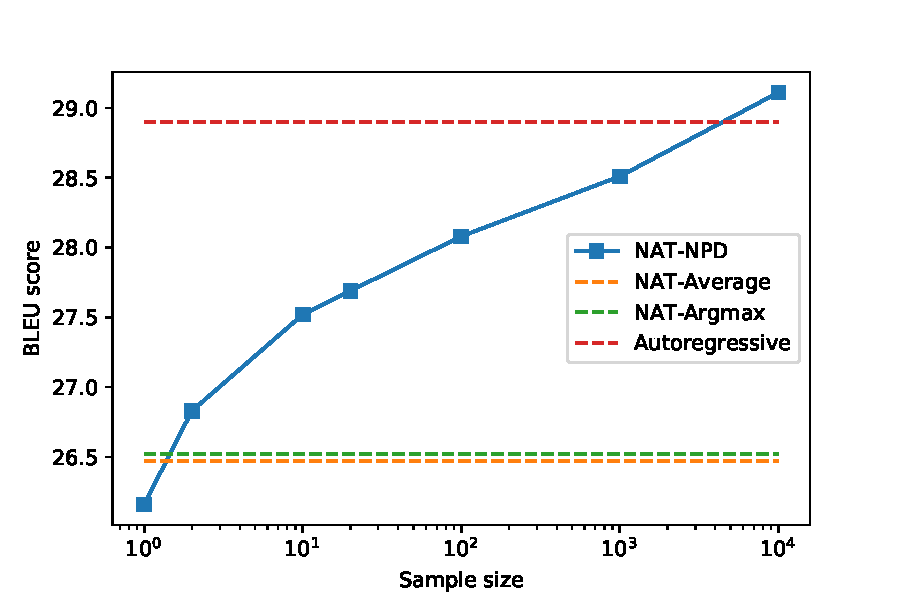
\includegraphics[width=0.8\linewidth]{figs/nat/NAT-sample-bleu}
\caption{\label{cp8.fig.noisy_decoding} BLEU scores on IWSLT development set as a function of sample size for noisy parallel decoding. NPD matches the performance of the other two decoding strategies after two samples, and exceeds the performance of the autoregressive teacher with around 1000.}
\end{figure}


\paragraph{Preparation for knowledge distillation} We first train all teacher models using maximum likelihood, then freeze their parameters. To avoid the redundancy of running fixed teacher models repeatedly on the same data, we decode the entire training set once using each teacher to create a new training dataset for its respective student.


\paragraph{Encoder initialization}
We find it helpful to initialize the weights in the NAT student's encoder with the encoder weights from its teacher, as the autoregressive and non-autoregressive models share the same encoder input and architecture.


\paragraph{Fertility supervision during training}
As described above, we supervise the fertility predictions at train time by using a fixed aligner as a fertility inference function. We use the \texttt{fast\_align}\footnote{https://github.com/clab/fast\_align} implementation of IBM Model 2 for this purpose, with default parameters
\citep{dyer2013simple}.


\paragraph{Hyperparameters}
For experiments on WMT datasets, we use the hyperparameter settings of the \texttt{base} Transformer model described in \citet{vaswani2017attention}, though without label smoothing. As IWSLT is a smaller corpus, and to reduce training time, we use a set of smaller hyperparameters ($d_{\text{model}}=287, d_{\text{hidden}}=507, n_{\text{layer}}=5, n_{\text{head}}=2$, and $t_\text{warmup}=746$) for all experiments on that dataset.
%the result of a limited hyperparameter search using the autoregressive model. 
For fine-tuning we use $\lambda=0.25$.


\paragraph{Evaluation} We evaluate using tokenized and cased BLEU scores~\citep{papineni2002bleu}.

\paragraph{Implementation} We have open-sourced our PyTorch implementation of the \model{}\footnote{https://github.com/salesforce/nonauto-nmt}.

\subsection{Results}
Across the three datasets we used, the \model{} performs between 2-5 BLEU points worse than its autoregressive teacher, with part or all of this gap addressed by the use of noisy parallel decoding. In the case of WMT16 English--Romanian, NPD improves the performance of our non-autoregressive model to within 0.2 BLEU points of the previous overall state of the art \citep{gehring2017convolutional}.

\begin{table}[t]
%\vspace{-4mm}
  \centering
  \resizebox{\textwidth}{!}{
    \begin{tabular}{l|cccc|crr}
    \toprule
    Models                  & \multicolumn{2}{c}{WMT14} & \multicolumn{2}{c|}{WMT16} & \multicolumn{2}{c}{IWSLT16} \\
    \multicolumn{1}{c}{}   & \multicolumn{1}{|c}{En$\rightarrow$De} & \multicolumn{1}{c}{De$\rightarrow$En} & \multicolumn{1}{c}{En$\rightarrow$Ro} & \multicolumn{1}{c|}{Ro$\rightarrow$En} & \multicolumn{1}{c}{En$\rightarrow$De} & \multicolumn{2}{c}{Latency / Speedup}  \\
    \midrule
    %\multirow{3}[5]{*}{\rotatebox{90}{Dev}} 
    
     
         \model{}                       & 17.35 & 20.62& 26.22 & 27.83&  25.20 & 39 ms & $15.6 \times$ \\
         
         \model{} (+FT)                 & 17.69& 21.47 & 27.29 & 29.06&  26.52 & 39 ms & $15.6 \times$\\
         
         
         \model{} (+FT + NPD $s=10$)     & 18.66 & 22.41& 29.02&  30.76 & 27.44 & 79 ms & $7.68 \times$\\
         
         \model{} (+FT + NPD $s=100$)    & 19.17 & 23.20 & 29.79&  \textbf{31.44}     & 28.16 & 257 ms & $2.36 \times$ \\
         \midrule
         Autoregressive ($b=1$)         & 22.71 & 26.39 & 31.35 & 31.03 & 28.89 & 408 ms & $1.49 \times$ \\
    	 Autoregressive ($b=4$)         & 23.45 & 27.02 & 31.91 & 31.76 & 29.70 & 607 ms & $1.00 \times$ \\
    		
    
    \bottomrule
    \end{tabular}
    }
     \caption{BLEU scores on official test sets (\texttt{newstest2014} for WMT En-De and \texttt{newstest2016} for WMT En-Ro) or the development set for IWSLT. NAT models without NPD use argmax decoding. Latency is computed as the time to decode a single sentence without minibatching, averaged over the whole test set; decoding is implemented in PyTorch on a single NVIDIA Tesla P100.}
  \label{cp8.table.bleu}%
%\end{wraptable}
\end{table}

Comparing latencies on the development model shows a speedup of more than a factor of 10 over greedy autoregressive decoding, or a factor of 15 over beam search.  Latencies for decoding with NPD, regardless of sample size, could be reduced to about 80ms by parallelizing across multiple GPUs because each sample can be generated, then scored, independently from the others.

\paragraph{Ablation Study}
We also conduct an extensive ablation study with the proposed \model{} on the IWSLT dataset. First, we note that the model fails to train when provided with only positional embeddings as input to the decoder. Second, we see that training on the distillation corpus rather than the ground truth provides a fairly consistent improvement of around 5 BLEU points. Third, switching from uniform copying of source inputs to fertility-based copying improves performance by four BLEU points when using ground-truth training or two when using distillation.



\begin{table}[hptb]
\small\centering
\begin{tabular}{cc|ccc|ccc|rr}
\toprule
\multicolumn{2}{c|}{Distillation}  & 
\multicolumn{2}{c}{Decoder Inputs} & 
\multirow{2}[2]{*}{+PosAtt}  & 
\multicolumn{3}{|c|}{Fine-tuning} & 
\multirow{2}[2]{*}{BLEU} & 
\multirow{2}[2]{*}{BLEU (T)}\\
           
$b$=1 &
$b$=4 &
+uniform & 
\multicolumn{1}{c}{+fertility} 
& 
& 
\multicolumn{1}{|c}{+$\mathcal{L}_\text{KD}$}  & 
+$\mathcal{L}_\text{BP}$ & 
+$\mathcal{L}_\text{RL}$ &   &\\

\midrule 
& &              &              & $\checkmark$  & & & & $\approx 2$ \\
& & $\checkmark$ &              & $\checkmark$  & & & & $16.51$\\
& &              & $\checkmark$ & $\checkmark$  & & & & $18.87$\\
\midrule


$\checkmark$&  & $\checkmark$ &              & $\checkmark$  & & & & $20.72$\\
&  $\checkmark$& $\checkmark$ &              & $\checkmark$  & & & & $21.12$ \\
$\checkmark$&  &              & $\checkmark$ &               & & & & $24.02$ & $43.91$ \\
$\checkmark$&  &              & $\checkmark$ & $\checkmark$  & & & & $25.20$ & $45.41$ \\
\midrule
$\checkmark$&  & $\checkmark$ &  & $\checkmark$& $\checkmark$ & $\checkmark$ & & $22.44$ \\
$\checkmark$&  &              & $\checkmark$ & $\checkmark$  & & & $\checkmark$ & $\times$ & $\times$\\
$\checkmark$&  &              & $\checkmark$ & $\checkmark$  & & $\checkmark$ & & $\times$ & $\times$\\
$\checkmark$&  &              & $\checkmark$ & $\checkmark$  & $\checkmark$ & $\checkmark$ &  & $25.76$ & $46.11$\\
$\checkmark$&  &              & $\checkmark$ & $\checkmark$  & $\checkmark$ & $\checkmark$ & $\checkmark$ & $ \textbf{26.52}$ & $\textbf{47.38}$\\
\bottomrule
\end{tabular}
\caption{Ablation performance on the IWSLT development set. BLEU (T) refers to the BLEU score on a version of the development set that has been translated by the teacher model. An $\times$ indicates that fine-tuning caused that model to get worse. When uniform copying is used as the decoder inputs, the ground-truth target lengths are provided. All models use argmax decoding.}
\end{table}

Fine-tuning does not converge with reinforcement learning alone, or with the $\mathcal{L}_\text{BP}$ term alone, but use of all three fine-tuning terms together leads to an improvement of around 1.5 BLEU points. Training the student model from a distillation corpus produced using beam search is similar to training from the greedily-distilled corpus.

\begin{figure}[htpb]
\includegraphics[width=\textwidth]{figs/nat/examples1}
\caption{\label{cp8.fig.ex} Two examples comparing translations produced by an autoregressive (AR) and non-autoregressive Transformer as well as the result of noisy parallel decoding with sample size 100. Repeated words are highlighted in gray.}
\end{figure}
\begin{figure}[htpb]
\centering
\includegraphics[width=\textwidth]{figs/nat/fertility_example2}
\caption{\label{cp8.fig.fer} A Romanian--English example translated with noisy parallel decoding. At left are eight sampled fertility sequences from the encoder, represented with their corresponding decoder input sequences. Each of these values for the latent variable leads to a different possible output translation, shown at right. The autoregressive Transformer then picks the best translation, shown in red, a process which is much faster than directly using it to generate output.}
\end{figure}

\begin{figure}[hptb]
\centering
\includegraphics[width=0.75\textwidth]{figs/nat/length_vs_latency}
\caption{\label{cp8.fig.latency}The translation latency, computed as the time to decode a single sentence without minibatching, for each sentence in the IWSLT development set as a function of its length. The autoregressive model has latency linear in the decoding length, while the latency of the NAT is nearly constant for typical lengths, even with NPD with sample size 10. When using NPD with sample size 100, the level of parallelism is enough to more than saturate the GPU, leading again to linear latencies.}
\end{figure}

\begin{figure}[hptb]
\centering
\includegraphics[width=0.75\textwidth]{figs/nat/learning_curve}
\caption{\label{cp8.fig.curve}Learning curves for training and fine-tuning of the \model{} on IWSLT. BLEU scores are on the development set.}
\end{figure}

\paragraph{Examples}
We include two examples of translations from the IWSLT development set in Fig.~\ref{cp8.fig.ex}.
Instances of repeated words or phrases, highlighted in gray, are most prevalent in the non-autoregressive output for the relatively complex first example sentence. Two pairs of repeated words in the first example, as well as a pair in the second, are not present in the versions with noisy parallel decoding, suggesting that NPD scoring using the teacher model can filter out such mistakes. The translations produced by the \model{} with NPD, while of a similar quality to those produced by the autoregressive model, are also noticeably more literal. 
We also show an example of the noisy parallel decoding process in Fig.~\ref{cp8.fig.fer}, demonstrating the diversity of translations that can be found by sampling.

\subsection{Analysis and Schematic}
We also show more detailed analysis and the overall schematic structure in this section as shown in Fig \ref{cp8.fig.latency}, \ref{cp8.fig.curve} and \ref{cp8.fig.sch}. 
\begin{figure}[hptb]
\centering
\includegraphics[width=0.75\textwidth]{figs/nat/NAT-overall}
\caption{\label{cp8.fig.sch}The schematic structure of training and inference for the \model. The ``distilled data'' contains target sentences decoded by the autoregressive model and ground-truth source sentences.}
\end{figure}



\section{Conclusion and Next Chapter}
In this chapter, we introduce a latent variable model for non-autoregressive machine translation that enables a decoder based on \citet{vaswani2017attention} to take full advantage of its exceptional degree of internal parallelism even at inference time. As a result, we enjoy translation latencies of one-tenth that of an equal-sized autoregressive model, while maintaining competitive BLEU scores. As the first attempt, the proposed method also biazes a new research direction to explore non-autoregressive decoding.

Although the proposed \model{} aims to overcome the fundamental restriction of the existing NMT models that rely on autoregressive decoding,
there still exists one situation of inefficiency in the decoding of all NMT models, that is,  real-time translation (or so-called simultaneous translation).
Since all the NMT models we discussed up to now (including the proposed \model{}) assumes the model to read the whole source sentence before starting to translate,  the MT system has to wait until the speaker finishes his words.
It is not suitable for cases where timing is very important, e.g. simultaneous translation in international events. In the next chapter, we will demonstrate one method which can do real-time translation using NMT.


  

\chapter{Simultaneous Neural Machine Translation}
\label{simul}

% what is simultaneous machine translation
Simultaneous translation, the task of translating content in real-time as it is produced, is an important tool for real-time understanding of spoken lectures or conversations \cite{fugen2007simultaneous,bangalore2012real}.
Different from the typical machine translation~(MT) task, in which translation quality is paramount, simultaneous translation requires balancing the trade-off between translation quality and time delay to ensure that users receive translated content in an expeditious manner \cite{mieno2015speed}.
% This is analogous to interpreters at international conferences, who are required to start translating a speaker' sentence before the whole sentence is complete.
A number of methods have been proposed to solve this problem, mostly in the context of phrase-based machine translation.
These methods are based on a \textit{segmenter}, which receives the input one word at a time, then decides when to send it to a MT system that translates each segment independently \cite{oda-EtAl:2014:P14-2} or with a minimal amount of language model context \cite{bangalore2012real}.
\begin{figure}[!t]
   	\centering
          	%\vspace{-10pt}
          	\includegraphics[width=\linewidth]{figs/simultrans/cropped_kkkk.pdf} 
          	\caption{\label{crop} {Example output from the proposed framework in DE $\rightarrow$ EN simultaneous translation. The heat-map represents the soft alignment between the incoming source sentence (left, up-to-down) and the emitted translation (top, left-to-right). The length of each column represents the number of source words being waited for before emitting the translation. Best viewed when zoomed digitally.}}
\end{figure} 

Independently of simultaneous translation, accuracy of standard MT systems has greatly improved with the introduction of neural-network-based MT systems (NMT)~\cite{sutskever2014sequence,bahdanau2014neural}.
Very recently, there have been a few efforts to apply NMT to simultaneous translation either through heuristic modifications to the decoding process \cite{cho2016can}, or through the training of an independent segmentation network that chooses when to perform output using a standard NMT model \cite{satija2016simultaneous}.
However, the former model lacks a capability to learn the appropriate timing with which to perform translation, and the latter model uses a standard NMT model as-is, lacking a holistic design of the modeling and learning within the simultaneous MT context.
In addition, neither model has demonstrated gains over previous segmentation-based baselines, leaving questions of their relative merit unresolved.

  
In this paper, we propose a unified design for learning to perform neural simultaneous machine translation.
The proposed framework is based on formulating translation as an interleaved sequence of two actions: \textsc{read} and \textsc{write}.
Based on this, we devise a model connecting the NMT system and these \textsc{read}/\textsc{write} decisions.
An example of how translation is performed in this framework is shown in Fig.~\ref{crop}, and detailed definitions of the problem and proposed framework are described in \S\ref{sec:definition} and \S\ref{sec:framework}.
To learn which actions to take when, we propose a reinforcement-learning-based strategy with a reward function that considers both quality and delay (\S\ref{sec:optimization}).
We also develop a beam-search method that performs search within the translation segments (\S\ref{sec:beamsearch}).

We evaluate the proposed method on English-Russian~(EN-RU) and English-German~(EN-DE) translation in both directions (\S\ref{sec:experiments}).
The quantitative results show strong improvements compared to both the NMT-based algorithm and a conventional segmentation methods.
We also extensively analyze the effectiveness of the learning algorithm and the influence of the trade-off in the optimization criterion, by varying a target delay.
Finally, qualitative visualization is utilized to discuss the potential and limitations of the framework.


\section{Problem Definition}
\label{sec:definition}
\vspace{-5pt}
% \paragraph{Simultaneous Machine Translation as Sequential Decision Making}
% \neu{The equation in this section doesn't make much sense to me, probably because ``quality'' and ``delay'' are not explicitly defined. Either explain this equation more carefully, or skip it until later when you can use more detail. Personally I'd like it to be described more explicitly, so a reader could literally look at the equations and implement something.}

Suppose we have a buffer of input words $X = \{x_1, ..., x_{T_s}\}$ to be translated in real-time. We define the simultaneous translation task as sequentially making two interleaved decisions: \textsc{read} or \textsc{write}.
More precisely, the translator \textsc{read}s a source word $x_\eta$ from the input buffer in chronological order as translation context, or \textsc{write}s a translated word $y_\tau$ onto the output buffer, resulting in output sentence $Y = \{y_1, ..., y_{T_t}\}$,
and action sequence $A=\{a_1, ..., a_T\}$ consists of $T_s$ \textsc{read}s and $T_t$ \textsc{write}s, so $T=T_s+T_t$.

Similar to standard MT, we have a measure $Q(Y)$ to evaluate the translation quality, such as BLEU score~\cite{papineni2002bleu}.
For simultaneous translation we are also concerned with the fact that each action incurs a time delay $D(A)$.
$D(A)$ will mainly be influenced by delay caused by \textsc{read}, as this entails waiting for a human speaker to continue speaking (about $0.3$s per word for an average speaker), while \textsc{write} consists of generating a few words from a machine translation system, which is possible on the order of milliseconds.
Thus, our objective is finding an optimal policy that generates decision sequences with a good trade-off between higher quality $Q(Y)$ and lower delay $D(A)$.
We elaborate on exactly how to define this trade-off in \S\ref{sec:reward}.

%Suppose the simultaneous translator consists of a \textsc{reader} and a \textsc{writer}. Given a stream of source words $X$, 
%\textsc{reader} reads words from the stream in chronological order, and \textsc{writer} writes the translation words one-by-one based on the instantaneous \textsc{reader}'s information. Naturally, the longer \textsc{writer} waits for \textsc{reader} to read more source words, the better translation quality it will tend to achieve. 
%Different from the usual machine translation situation, in our case each decision $\{\textsc{read}, \textsc{write}\}$ will incur a time cost, or delay, which leads to the objective of finding an optimal decision sequence $\hat{A} = \{a_1, a_2, ... a_T\}$ and resulting translation $Y$: 
% \vspace{-5pt}
% \begin{equation}
%     \hat{A} = \arg_{A}\{\max Q(Y|A), \min\mathcal{T}(A)\}
%     \vspace{-5pt}
%     \label{problem}
% \end{equation}

%\vspace{-10pt}

In the following sections, we first describe how to connect the \textsc{read}/\textsc{write} actions with the NMT system (\S\ref{sec:framework}), and how to optimize the system to improve simultaneous MT results (\S\ref{sec:optimization}).
% Apparently, we can easily find a straightforward connection between the discussed actions (\textsc{read} and the encoder, \textsc{write} and the decoder) in the context of NMT. Focusing on the trade-off objectives of Eq.~\ref{problem}, a generic NMT-based simultaneous translation framework is proposed in Section~\ref{sec:framework}. 

%\paragraph{Neural Machine Translation as Interactive Internal Environment}~ 
%\neu{The description in this section is pretty difficult to understand. Do we really need this section at all?}
%Recently sequence-to-sequence learning based NMT (NMT)~\cite{sutskever2014sequence,bahdanau2014neural} has showed promising achievements and become a major alternative to existing machine translation systems~\cite{sennrich-haddow-birch:2016:WMT}. Typically an NMT system is seen as a composite of two modules: \textsc{encoder} and \textsc{decoder}, both of which can be built and trained using recurrent neural networks (RNNs). 
%Not surprisingly, we can find a strong connection between the \textsc{encoder-decoder} and the \textsc{reader-writer} of simultaneous translation, implying that we can directly apply an existing NMT system to do simultaneous machine translation~\cite{cho2016can}. More precisely, the trained NMT system is treated as an interactive environment, upon which an agent receives its output, makes decisions and sends decisions back to control the translation. 
%We call this general framework as ``Simultaneous Neural Machine Translation" and our objective is to find an optimal agent that produces best decision sequence depending on the source streams. In this paper, we solve this optimization problem via reinforcement learning techniques.


\section{Simultaneous Translation \\ with Neural Machine Translation}
\label{sec:framework}

%\neu{There is no reference to reader/writer in this section, so the connection with the previous section is not so clear. Can we make this flow more smoothly?}
% In this section, we introduce the details of the proposed framework for simultaneous translation using NMT systems. 
The proposed framework is shown in Fig.~\ref{snmt}, and can be naturally decomposed into two parts: environment (\S\ref{sec:environment}) and agent (\S\ref{sec:agent}).
%We can design the specific decoding algorithm based on the agent behavior.
\begin{figure}[hptb]
   	\centering
          	\includegraphics[width=\linewidth]{figs/simultrans/SNMT.pdf} 
          	\caption{\label{snmt} {Illustration of the proposed framework: at each step, the NMT environment (left) computes a candidate translation. The recurrent agent (right) will the observation including the candidates and send back decisions--\textsc{read} or \textsc{write}.}} 
  \end{figure} 
  
\subsection{Environment}
\label{sec:environment}
\paragraph{Encoder:~\textsc{read}} 
The first element of the NMT system is the encoder, which converts input words $X=\{x_1, ..., x_{T_s}\}$ into context vectors $H = \{h_1, ..., h_{T_s}\}$.
Standard NMT uses bi-directional RNNs as encoders \cite{bahdanau2014neural}, but this is not suitable for simultaneous processing as using a reverse-order encoder requires knowing the final word of the sentence before beginning processing.
Thus, we utilize a simple left-to-right uni-directional RNN as our encoder:

\begin{equation}
\label{enc}
    h_{\eta} = \phi_{\textsc{uni-enc}}\left(h_{\eta-1}, x_{\eta}\right)
\end{equation}

\paragraph{Decoder:~\textsc{write}} Similar with standard MT, we use an attention-based decoder. In contrast, we only reference the words that have been read from the input when generating each target word:

\begin{equation}
\label{dec}
    \begin{split}
        &c_{\tau}^{\eta} = \phi_{\textsc{att}}\left(z_{\tau-1}, y_{\tau-1}, H^{\eta}\right) \\
        &z_{\tau}^{\eta} = \phi_{\textsc{dec}}\left(z_{\tau-1}, y_{\tau-1}, c_{\tau}^{\eta}\right)\\
        &p\left(y|y_{<\tau}, H^{\eta}\right) \propto \exp\left[\phi_{\textsc{out}}\left(z_{\tau}^{\eta}\right)\right],
    \end{split}
\end{equation}
where for $\tau$, $z_{\tau-1}$ and $y_{\tau-1}$ represent the previous decoder state and output word, respectively.
$H^{\eta}$ is used to represent the incomplete input states, where $H^{\eta}$ is a prefix of $H$.  % $z_0$ is initialized by the source.
%Unlike common NMT systems that run decoding with Beam search for the best quality of translation, 
% Based on this definition, 
As the \textsc{write} action calculates the probability of the next word on the fly, we need greedy decoding for each step:
\vspace{-5pt}
\begin{equation}
    y_{\tau}^{\eta} = \argmax\nolimits_{y}p\left(y|y_{<\tau}, H^{\eta}\right) 
\vspace{-2pt}
\end{equation}
Note that $y_{\tau}^{\eta}, z_{\tau}^{\eta}$ corresponds to $H^{\eta}$ and is the candidate for $y_{\tau}, z_{\tau}$.
The agent described in the next section decides whether to take this candidate or wait for better predictions.

\subsection{Agent}
\label{sec:agent}
A trainable agent is designed to make decisions $A=\{a_1, .., a_T\}, a_t \in \mathcal{A}$ sequentially based on observations $O=\{o_1, ..., o_T\}, o_t \in \mathcal{O}$, and then control the translation environment properly. %In our case, the dynamics must be fixed for policy learning. 
\paragraph{Observation} As shown in Fig~\ref{snmt}, we concatenate the current context vector $c_{\tau}^{\eta}$, the current decoder state $z_{\tau}^{\eta}$ and the embedding vector of the candidate word $y_{\tau}^{\eta}$ as the continuous observation, $o_{\tau+\eta}=\left[c_{\tau}^{\eta}; z_{\tau}^{\eta}; E(y_{\tau}^{\eta})\right]$ to represent the current state.% of the environment.

\paragraph{Action} Similarly to prior work~\cite{grissomii2014don}, we define the following set of actions:
\begin{itemize}[leftmargin=*]
	\itemsep -0.4em
    \item \textbf{\textsc{read}}: the agent rejects the candidate and waits to encode the next word from input buffer;
    \item \textbf{\textsc{write}}: the agent accepts the candidate and emits it as the prediction into output buffer;
\end{itemize}
% Clearly we can use a discrete boolean $a \in \{0, 1\}$ to represent the above decisions.

\paragraph{Policy} How the agent chooses the actions based on the observation defines the policy. In our setting, we utilize a stochastic policy $\pi_{\theta}$ parameterized by a recurrent neural network, that is:

\begin{equation}
    \begin{split}
        &s_t = f_{\theta}\left(s_{t-1}, o_t\right)\\
        &\pi_{\theta}(a_t|a_{<t}, o_{\leq t}) \propto g_{\theta}\left(s_t\right), 
    \end{split}
\end{equation}
where $s_t$ is the internal state of the agent, and is updated recurrently yielding the distribution of the action $a_t$. 
Based on the policy of our agent, the overall algorithm of greedy decoding is shown in Algorithm~\ref{algo1}, %where the policy is learned to make use of the fixed NMT system, and decisions are made. 
%where the single-line arrows represent "assign values", and double-line arrows represent "an element pull from or push to the buffer".
The algorithm outputs the translation result and a sequence of observation-action pairs.


\begin{algorithm}
\caption{Simultaneous Greedy Decoding}
\label{algo1}
\begin{algorithmic}[1]
%\small
\Require{NMT system $\phi$, policy $\pi_{\theta}$, $\tau_{\textsc{max}}$, input buffer $X$, output buffer $Y$, state buffer $S$.}
\State \textbf{Init} $x_1 \Leftarrow X, h_1 \gets \phi_{\textsc{enc}}\left(x_1\right), H^1 \gets \{h_1\}$
\State \hspace{17pt} $z_0 \gets \phi_{\textsc{init}}\left(H^1\right), y_0 \gets \left<s\right>$
\State \hspace{17pt} $\tau \gets 0, \eta \gets 1$
\While{$\tau < {\tau}_{\textsc{max}}$}
\State $t \gets \tau + \eta$
\State $y_{\tau}^{\eta}, z_{\tau}^{\eta}, o_t \gets \phi\left(z_{\tau-1}, y_{\tau-1}, H^{\eta}\right)$ 
\State $a_t \sim \pi_{\theta}\left(a_t; a_{<t}, o_{<t}\right), S \Leftarrow (o_t, a_t)$
\If {$a_t=\textsc{read}$ and $x_{\eta} \neq \left</s\right>$}
\State $x_{\eta+1} \Leftarrow X, h_{\eta+1} \gets \phi_{\textsc{enc}}\left(h_{\eta}, x_{\eta+1}\right)$
\State $H^{\eta+1} \gets H^{\eta} \cup \{h_{\eta+1} \}, \eta \gets \eta + 1$
\If {$|Y|=0$} $z_0 \gets \phi_{\textsc{init}}\left(H^{\eta}\right)$
\EndIf
\ElsIf {$a_t = \textsc{write}$}
\State $z_{\tau} \gets z_{\tau}^{\eta}, y_{\tau} \gets y_{\tau}^{\eta}$ 
\State $Y \Leftarrow y_{\tau}, \tau \gets \tau + 1$
\If {$y_{\tau}=\left</s\right>$} \textbf{break}
\EndIf
\EndIf
\EndWhile
\end{algorithmic}
\end{algorithm}

\section{Learning}
\label{sec:optimization}
The proposed framework can be trained using reinforcement learning. More precisely, we use policy gradient algorithm together with variance reduction and regularization techniques.
%\vspace{-3pt}
\subsection{Pre-training} 
We need an NMT environment for the agent to explore and use to generate translations.
% Unfortunately, it is almost impossible to obtain an accurate decoder for incomplete source words as required in Eq.~\ref{dec} due to the lack of corresponding training examples for partial translation. 
Here, we simply pre-train the NMT encoder-decoder on full sentence pairs with maximum likelihood, and assume the pre-trained model is still able to generate reasonable translations even on incomplete source sentences.
Although this is likely sub-optimal, our NMT environment based on uni-directional RNNs can treat incomplete source sentences in a manner similar to shorter source sentences and has the potential to translate them more-or-less correctly.% In addition, an imperfect decoder makes it easier for the agent to make decis

% We need a fixed and reliable NMT environment for the agent to explore and make a decision. Unfortunately, it is almost impossible to obtain an accurate decoder for incomplete source words as required in Eq.~\ref{dec} due to the lack of corresponding training examples for partial translation. 

% Instead, we pre-train the NMT encoder-decoder on complete sentence pairs with maximum likelihood, and assume the trained model is still able to generate reasonable translation even on incomplete source sentences. Although this configuration is not optimal, in our NMT environment, %which is based on uni-directional RNNs, 
% incomplete source sentences can still be treated as shorter sentences and translated.% In addition, an imperfect decoder makes it easier for the agent to make decisions and find the policy.

\subsection{Reward Function}
\label{sec:reward}

The policy is learned in order to increase a reward for the translation. At each step the agent will receive a reward signal $r_t$ based on $(o_t, a_t)$. To evaluate a good simultaneous machine translation, a reward must consider both quality and delay. 

\paragraph{Quality} We evaluate the translation quality using metrics such as BLEU~\cite{papineni2002bleu}. The BLEU score is defined as the weighted geometric average of the modified n-gram precision $\textsc{BLEU}^0$, multiplied by the brevity penalty $\textsc{BP}$ to punish a short translation. In practice, the vanilla BLEU score is not a good metric at sentence level because being a geometric average, the score will reduce to zero if one of the precisions is zero. To avoid this, we used a smoothed version of BLEU for our implementation~\cite{lin2004automatic}.

\begin{equation}
    \textsc{BLEU}(Y, Y^*) = \textsc{BP} \cdot \textsc{BLEU}^0(Y, Y^*),
\end{equation}
where $Y^*$ is the reference and $Y$ is the output.  
We decompose $\textsc{BLEU}$ and use the difference of partial $\textsc{BLEU}$ scores as the reward, that is:
\begin{equation}
    r_t^Q=\left\{
\begin{array}{rcl}
\Delta\textsc{BLEU}^0(Y, Y^*, t)     &      & {t < T}\\
\textsc{BLEU}(Y, Y^*)    &      & {t = T}
\end{array} \right. 
\end{equation}
where $Y^t$ is the cumulative output at $t$ ($Y^0=\emptyset$), and $\Delta\textsc{BLEU}^0(Y, Y^*, t) = \textsc{BLEU}^0(Y^t, Y^*) - \textsc{BLEU}^0(Y^{t-1}, Y^*)$. Obviously, if $a_t=\textsc{read}$, no new words are written into $Y$, yielding $r_t^Q=0$. Note that we do not multiply $\textsc{BP}$
until the end of the sentence, as it would heavily penalize partial translation results.

\paragraph{Delay}As another critical feature, delay judges how much time is wasted waiting for the translation. Ideally we would directly measure the actual time delay incurred by waiting for the next word. For simplicity, however, we suppose it consumes the same amount of time listening  for one more word. We define two measurements, global and local, respectively:

\begin{itemize}[leftmargin=*]
    \item \textbf{Average Proportion (AP)}: following the definition in \cite{cho2016can}, $X$, $Y$ are the source and decoded sequences respectively, and we use $s(\tau)$ to denote the number of source words been waited when decoding word $y_\tau$, 

    \begin{equation}
    \begin{split}
        &0 < d\left(X, Y\right) = \frac{1}{|X||Y|}\sum_{\tau}{s(\tau)}\leq 1 \\
        &d_t = 
        \left\{\begin{array}{ll}
        0    &     t < T\\
        d(X, Y)  &     t = T
        \end{array} \right. 
    \end{split}
    \end{equation}
    $d$ is a global delay metric, which defines the average waiting proportion of the source sentence when translating each word.\vspace{-5pt}
    \item \textbf{Consecutive Wait length (CW)}: in speech translation, listeners are also concerned with long silences during which no translation occurs. To capture this, we also consider on how many words were waited for (\textsc{read}) consecutively between translating two words. For each action, where we initially define $c_0=0$,

    \begin{equation}
        c_t = 
        \left\{\begin{array}{ll}
        c_{t-1} + 1    &     a_t = \textsc{read}\\
        0             &      a_t = \textsc{write}
        \end{array} \right.         
    \end{equation}
\item \textbf{Target Delay:}~
We further define ``target delay" for both $d$ and $c$ as $d^*$ and $c^*$, respectively, as different simultaneous translation applications may have different requirements on delay. In our implementation, the reward function for delay is written as:

\begin{equation}
    \label{eq_rd}
    r_t^{D} = \alpha \cdot \left[\text{sgn}(c_t - c^*)+1\right] + \beta \cdot \lfloor d_t - d^* \rfloor_{+}
\end{equation}
where $\alpha \leq 0, \beta \leq 0$. 
\end{itemize}

\paragraph{Trade-off between quality and delay}
A good simultaneous translation system requires balancing the trade-off of translation quality and time delay. Obviously, achieving the best translation quality and the shortest translation delays are in a sense contradictory. In this paper, the trade-off is achieved by balancing the rewards $r_t = r_t^Q + r_t^D$ provided to the system, that is, by adjusting the coefficients $\alpha,\beta$ and the target delay $d^*, c^*$ in Eq.~\ref{eq_rd}. 

\subsection{Reinforcement Learning}

\paragraph{Policy Gradient}
We freeze the pre-trained parameters of an NMT model, and train the agent using the policy gradient~\cite{williams1992simple}. The policy gradient maximizes the following expected cumulative future rewards,
%\begin{equation}
%\begin{split}
$     J = \mathbb{E}_{\pi_{\theta}}\left[\sum_{t=1}^T r_t\right], $ whose gradient is 
%\end{split}
%\end{equation}
%Its gradient is then, 
\begin{equation}
\label{eq.train}
   \nabla_{\theta}J=\mathbb{E}_{\pi_{\theta}}\left[\sum_{t'=1}^T\nabla_{\theta}\log \pi_{\theta}(a_{t'}|\cdot) R_t\right]
\end{equation}
$R_t=\sum_{k=t}^T\left[r_k^Q + r_k^D\right]$ is the cumulative future rewards for current observation and action. %The overall learning algorithm can be seen as follows:
In practice, Eq.~\ref{eq.train} is estimated by sampling multiple action trajectories from the current policy $\pi_{\theta}$, collecting the corresponding rewards.

\paragraph{Variance Reduction}~
Directly using the policy gradient suffers from high variance, which makes learning unstable and inefficient. We thus employ the variance reduction techniques suggested by~\citep{mnih2014neural}. We subtract from $R_t$ the output of a baseline network $b_{\varphi}$ to obtain $\hat{R}_t = R_t - b_{\varphi}\left(o_t\right)$, and centered re-scale the reward as $\tilde{R}_t = \frac{\hat{R}_t - b}{\sqrt{\sigma^2+\epsilon}}$ with a running average $b$ and standard deviation $\sigma$. The baseline network is trained to minimize the squared loss as follows:

\begin{equation}
    L_{\varphi} = \mathbb{E}_{\pi_{\theta}}\left[ \sum_{t=1}^T\|R_t - b_{\varphi}\left(o_t\right)\|^2 \right]
\end{equation}

%\neu{Do you have a reference for this? I'd suggest citing it. Also, if this is one of the things that you needed to do to get it to work properly, I'd suggest stressing this a little more as one of the insights of our paper.}
%\paragraph{Regularization} 
We also regularize the negative entropy of  the policy 
%distribution 
%$\mathcal{H}\left(\pi_{\theta}\right)$ 
to facilitate exploration. 
%\vspace{5pt}
%\\ 

The overall learning algorithm is summarized in Algorithm~\ref{algo2}. For efficiency, instead of updating with stochastic gradient descent~(SGD) on a single sentence, both the agent and the baseline are optimized using 
%the Adam~\cite{kingma2014adam} on 
a minibatch of multiple sentences.

\begin{algorithm}[t]
\caption{Learning with Policy Gradient}
\label{algo2}
\begin{algorithmic}[1]
%\small
\Require{NMT system $\phi$, agent $\theta$, baseline $\varphi$}
\State Pretrain the NMT system $\phi$ using MLE;
\State Initialize the agent $\theta$;
\While{stopping criterion fails}
\State Obtain a translation pairs: $\{(X, Y^*)\}$;
\For{$(Y, S) \sim$ Simultaneous Decoding}
\For{$(o_t, a_t)$ in $S$}
\State Compute the quality: $r_t^Q$;
\State Compute the delay: $r_t^D$;
\State Compute the baseline: $b_{\varphi}\left(o_t\right)$;
\EndFor
\EndFor
\State Collect the future rewards: $\{R_t\}$;
\State Perform variance reduction: $\{\tilde{R}_t\}$;
\State Update: $\theta \gets \theta + \lambda_1 \nabla_{\theta}\left[J - \kappa\mathcal{H}(\pi_{\theta})\right]$
\State Update: $\varphi \gets \varphi - \lambda_2 \nabla_{\varphi}L$
\EndWhile
\end{algorithmic}
\end{algorithm}


\section{Simultaneous Beam Search}
\label{sec:beamsearch}

In previous sections we described a simultaneous greedy decoding algorithm. In standard NMT it has been shown that beam search, where the decoder keeps a beam of $k$ translation trajectories, greatly improves translation quality~\cite{sutskever2014sequence}, as shown in Fig.~\ref{beam}\,(A). 
%the final output is determined by choosing the best translation from the whole beams.

It is non-trivial to directly apply beam-search in simultaneous machine translation,
as beam search waits until the last word to write down translation. Based on our assumption \textsc{write} does not cost delay,
we can perform a simultaneous beam-search when the agent chooses to consecutively \textsc{write}: keep multiple beams of translation trajectories in temporary buffer and output the best path when the agent switches to \textsc{read}. As shown in Fig.~\ref{beam} (B) \& (C), it tries to search for a relatively better path while keeping the delay unchanged.

\begin{figure}[t]
   	\centering
          	
          	\includegraphics[width=\linewidth]{figs/simultrans/decoding.pdf} 
          	%\vspace{-15pt}
          	\caption{\label{beam} {Illustrations of (A)~beam-search, (B)~simultaneous greedy decoding and (C)~simultaneous beam-search.}} 
  
\end{figure} 

Note that we do not re-train the agent for simultaneous beam-search. At each step we simply input the observation of the current best trajectory into the agent for making next decision. %As it is not optimal, we will leave the better choice of alternating the beam-search in future work.



\section{Experiments}
\label{sec:experiments}
% \subfigure[BLEU (RU $\rightarrow$ EN)]{
% \includegraphics[width=.31\textwidth]{lr_ruen_BLEU.pdf}
% }
% \subfigure[AP (RU $\rightarrow$ EN)]{
% \includegraphics[width=.31\textwidth]{lr_ruen_DELAY.pdf}
% }
% \subfigure[CW (RU $\rightarrow$ EN)]{
% \includegraphics[width=.31\textwidth]{lr_ruen_WAIT.pdf}
% }
\begin{figure*}[hptb]
\centering
\subfigure[BLEU (EN $\rightarrow$ RU)]{
\includegraphics[width=0.7\textwidth]{figs/simultrans/lr_enru_BLEU.pdf}
}
\subfigure[AP (EN $\rightarrow$ RU)]{
\includegraphics[width=0.7\textwidth]{figs/simultrans/lr_enru_DELAY.pdf}
}
\subfigure[CW (EN $\rightarrow$ RU)]{
\includegraphics[width=0.7\textwidth]{figs/simultrans/lr_enru_WAIT.pdf}
}

\caption{{Learning progress curves for variant delay targets on the validation dataset for EN $\rightarrow$ RU. Every time we only keep one target for one delay measure. For instance when using target AP, the coefficient of $\alpha$ in Eq.~\ref{eq_rd} will be set $0$.}}
\label{fig.lr}
\vspace{-7pt}
\end{figure*}

\begin{figure*}[hptb]
\centering
\subfigure[EN$\rightarrow$RU]{
\includegraphics[width=0.47\textwidth]{figs/simultrans/lr_enru_DELAY_vs_BLEU.pdf}
}
\hfill
\subfigure[RU$\rightarrow$EN]{
\includegraphics[width=0.47\textwidth]{figs/simultrans/lr_ruen_DELAY_vs_BLEU.pdf}
}
\hfill
\subfigure[EN$\rightarrow$DE]{
\includegraphics[width=0.47\textwidth]{figs/simultrans/lr_ende_DELAY_vs_BLEU.pdf}
}
\hfill
\subfigure[DE$\rightarrow$EN]{
\includegraphics[width=0.47\textwidth]{figs/simultrans/lr_deen_DELAY_vs_BLEU.pdf}
}

\hfill
\caption{{Delay~(AP) v.s. BLEU for both language pair--directions. The shown point-pairs are the results of simultaneous greedy decoding and beam-search (beam-size = 5) respectively with models trained for various delay targets: ($\color{green!70!blue}\blacktriangleleft\triangleleft$:   CW=$8$,
 $\color{green!70!blue}\blacktriangle\triangle$:           CW=$5$,
 $\color{green!70!blue}\blacklozenge\lozenge$:             CW=$2$,
 $\color{red}  \blacktriangleright\triangleright$: AP=$0.3$,
 $\color{red}  \blacktriangledown\triangledown$:   AP=$0.5$,
 $\color{red}  \blacksquare\square$:               AP=$0.7$)}. For each target, we select the model that maximizes the quality-to-delay ratio ($\frac{\text{BLEU}}{\text{AP}}$) on the validation set. The baselines are also plotted ($\color{blue}\bigstar$: WOS $\color{black}\bigstar$\ding{73}: WUE, $\times$: WID, $+$: WIW).}

\label{fig.bvd}
\hfill

\end{figure*}

\begin{figure}[hptb]
   	\centering
          	%\vspace{-10pt}
          	\includegraphics[width=\linewidth]{figs/simultrans/lr_enru_WAIT_vs_BLEU.pdf} 
          
          	\caption{\label{wait} {Delay~(CW) v.s. BLEU score for EN $\rightarrow$ RU,
($\color{green!70!blue}\blacktriangleleft\triangleleft$:   CW=$8$,
 $\color{green!70!blue}\blacktriangle\triangle$:           CW=$5$,
 $\color{green!70!blue}\blacklozenge\lozenge$:             CW=$2$,
 $\color{red}  \blacktriangleright\triangleright$: AP=$0.3$,
 $\color{red}  \blacktriangledown\triangledown$:   AP=$0.5$,
 $\color{red}  \blacksquare\square$:               AP=$0.7$), against the baselines~($\color{blue}\bigstar$: WOS $\color{black}\bigstar$: WUE, $+$: SEG1, $\times$: SEG2).}} 

\end{figure} 

\subsection{Settings}
\paragraph{Dataset}~
To extensively study the proposed simultaneous translation model, we train and evaluate it on two different language pairs: ``English-German (EN-DE)" and ``English-Russian (EN-RU)" in both directions per pair. We use the parallel corpora available from WMT'15\footnote{http://www.statmt.org/wmt15/} for both pre-training the NMT environment and learning the policy. We utilize newstest-2013 as the validation set to evaluate the proposed algorithm. Both the training set and the validation set are tokenized and segmented into sub-word units with byte-pair encoding (BPE)~\cite{sennrich2015neural}. We only use sentence pairs where both sides are less than 50 BPE subword symbols long for training.

\paragraph{Environment \& Agent Settings}
We pre-trained the NMT environments for both language pairs and both directions following the same setting from~\cite{cho2016can}. % with the same network architecture, which consists of an unidirectional RNN Encoder and an attention-based RNN Decoder. Both the encoder and decoder contain 1028 gated recurrent units (GRUs)~\cite{cho2014learning}. The embedding dimensions for both source and target words are 512. Each model takes 1 week to optimize using Adadelta~\cite{zeiler2012adadelta} on single Nvidia Titan X. 
We further built our agents, using a recurrent policy with 512 GRUs and a softmax function to produce the action distribution. All our agents are trained using policy gradient using Adam~\cite{kingma2014adam} optimizer, with a mini-batch size of 10. For each sentence pair in a batch, 5 trajectories are sampled. 
For testing, instead of sampling we pick the action with higher probability each step.

%In all, 50 observation-action trajectories are sampled for computing policy gradient per mini-batch.


\paragraph{Baselines}~ We compare the proposed methods against previously proposed baselines.
For fair comparison, we use the same NMT environment:
\begin{itemize}[leftmargin=*]

\item \textbf{Wait-Until-End (WUE)}: an agent that starts to \textsc{write} only when the last source word is seen. In general, we expect this to achieve the best quality of translation. We perform both greedy decoding and beam-search with this method.

\item \textbf{Wait-One-Step (WOS)}: an agent that \textsc{write}s after each \textsc{read}s. %Obviously, it will achieve the best ``consecutive waiting length", however, 
Such a policy is problematic when the source and target language pairs have different word orders or lengths (e.g. EN-DE). %sentences have different lengths.

\item \textbf{Wait-If-Worse/Wait-If-Diff (WIW/WID)}: as proposed by \citep{cho2016can}, the algorithm first pre-\textsc{read}s the next source word, and accepts this \textsc{read} when the probability of the most likely target word decreases~(WIW), or the most likely target word changes~(WID). 

\item \textbf{Segmentation-based (SEG)}~\cite{oda-EtAl:2014:P14-2}: a state-of-the-art segmentation-based algorithm based on optimizing segmentation to achieve the highest quality score. In this paper, we tried the simple greedy method~(SEG1) and the greedy method with POS Constraint~(SEG2).
\end{itemize}

\subsection{Quantitative Analysis}

In order to evaluate the effectiveness of our reinforcement learning algorithms with different reward functions, we vary the target delay $d^* \in \{0.3, 0.5, 0.7\}$ and $c^* \in \{2, 5, 8\}$ for Eq.~\ref{eq_rd} separately, and trained agents with $\alpha$ and $\beta$ adjusted to values that provided stable learning for each language pair according to the validation set.

\paragraph{Learning Curves}~ As shown in Fig.~\ref{fig.lr}, we plot learning progress for EN-RU translation with different target settings. It clearly shows that our algorithm effectively increases translation quality for all the models, while pushing the delay close, if not all of the way, to the target value.
% Note that when targeting average proportion (AP), in order to balance the quality and delay the algorithm cannot accurately push the output to achieve the target. % In contrast, it seems easier to use consecutive waited length (CW) because of the usage of instant reward during training.
It can also be noted from Fig.~\ref{fig.lr} (a) and (b) that there exists strong correlation between the two delay measures, implying the agent can learn to decrease both AP and CW simultaneously.

\paragraph{Quality v.s. Delay}~ As shown in Fig.~\ref{fig.bvd}, it is clear that the trade-off between translation quality and delay has very similar behaviors across both language pairs and directions. The smaller delay (AP or CW) the learning algorithm is targeting, the lower quality (BLEU score) the output translation. It is also interesting to observe that, it is more difficult for ``$\rightarrow$EN'' translation to achieve a lower AP target while maintaining good quality, compared to ``EN$\rightarrow$''. 
In addition, the models that are optimized on AP tend to perform better than those optimized on CW, especially in ``$\rightarrow$EN'' translation. German and Russian sentences tend to be longer than English, hence require more consecutive waits before being able to emit the next English symbol.

% This is likely because English has much shorter words than the other languages, and in turn less symbols.
% This requires longer consecutive waiting before getting enough symbols to translate, rendering CW targeting difficult.

\paragraph{v.s. Baselines}~
In Fig.~\ref{fig.bvd} and~\ref{wait}, %we visualize the results for all baseline models, for the purpose of showing the effectiveness of the proposed framework. Throughout all these figures, 
the points closer to the upper left corner achieve better trade-off performance. 
Compared to WUE and WOS which can ideally achieve the best quality (but the worst delay) and the best delay (but poor quality) respectively, all of our proposed models find a good balance between quality and delay.  Some of the proposed models can achieve good BLEU scores close to WUE, while have much smaller delay.
%Compared to EN-RU in which English and Russian share the same word orders, EN-DE is more challenging as order English and German usually are different.
%Note that the quality scores between the proposed models and WUE are more close in EN-RU than EN-DE.
%It is notable that in Fig~\ref{fig.bvd}~(a), the model for AP=0.3 achieves a smaller delay and much better quality than WOS; the model for CW=5 works with almost the same quality with WUE, but much smaller delay, which indicates that the proposed learning based framework can efficiently approach to ideal cases.


Compared to the method of \citep{cho2016can} based on two hand-crafted rules (WID, WIW), in most cases our proposed models find better trade-off points, while there are a few exceptions. We also observe that the baseline models have trouble controlling the delay in a reasonable area. In contrast, by optimizing towards a given target delay, our proposed model is stable while maintaining good translation quality.
  
We also compared against \citep{oda-EtAl:2014:P14-2}'s state-of-the-art segmentation algorithm (SEG). As shown in Fig~\ref{wait}, it is clear that although SEG can work with variant segmentation lengths (CW), 
the proposed model outputs high quality translations at a much smaller CW. 
We conjecture that this is due to the independence assumption in SEG,
while the RNNs and attention mechanism in our model makes it possible to look at the whole history to decide each translated word.

\paragraph{w/o Beam-Search}
We also plot the results of simultaneous beam-search instead of using greedy decoding. 
It is clear from Fig.~\ref{fig.bvd} and \ref{wait} that most of the proposed models can achieve an visible increase in quality together with a slight increase in delay. 
This is because beam-search can help to avoid bad local minima.  %can help to avoid early ending before reading up the source sentence.
We also observe that the simultaneous beam-search cannot bring as much improvement as it did in the standard NMT setting. In most cases, the smaller delay the model achieves, the less beam search can help as it requires longer consecutive \textsc{write} segments for extensive search to be necessary.
%\jtg{it has some problem to say this, as RU->EN low delay has a large improvement. I don't know how to explain this yet.}
One possible solution is to consider the beam uncertainty in the agent's \textsc{read/write} decisions. We leave this to future work. 

\subsection{Qualitative Analysis}
\begin{figure*}[hptb]
\centering
\subfigure[Simultaneous Neural Machine Translation]{
\includegraphics[width=\textwidth]{figs/simultrans/simultaneous.pdf}
}
\subfigure[Neural Machine Translation]{
\includegraphics[width=\textwidth]{figs/simultrans/greedy.pdf}
}
%\vspace{-5pt}
\caption{\label{deen2}{Comparison of DE$\rightarrow$EN examples using the proposed framework and usual NMT system respectively. Both the heatmaps share the same setting with Fig.~\ref{crop}}. The verb ``gedeckt'' is incorrectly translated in simultaneous translation.}
\end{figure*}

\begin{figure*}[hptb]
   	\centering
          	%\vspace{-10pt}
  	\includegraphics[width=\linewidth]{figs/simultrans/example_c2.pdf} 
          	%\vspace{-4mm}
          	\caption{\label{exp1} {Given the example input sentence (leftmost column), we show outputs by models trained for various delay targets. For these outputs, each row corresponds to one source word and represents the emitted words (maybe empty) after reading this word. The corresponding source and target words are in the same color for all model outputs.}}
          	%\vspace{-4mm}
\end{figure*} 

In this section, we perform a more in-depth analysis using examples from both EN-RU and EN-DE pairs, in order to have a deeper understanding of the proposed algorithm and its remaining limitations. We only perform greedy decoding to simplify visualization. 

\paragraph{EN$\rightarrow$RU}~ As shown in Fig~\ref{exp1}, since both English and Russian are Subject-–Verb-–Object~(SVO) languages, the corresponding words may share the same order in both languages, which makes simultaneous translation easier. 
It is clear that the larger the target delay (AP or CW) is set, the more words are read before translating the corresponding words, which in turn results in better translation quality. 
We also note that very early \textsc{write} commonly causes bad translation. For example, for AP=0.3 \& CW=2, both the models choose to \textsc{write} in the very beginning the word ``The'', which is unreasonable since Russian has no articles, and there is no word corresponding to it. One good feature of using NMT is that the more words the decoder \textsc{read}s, the longer history is saved, rendering simultaneous translation easier.

% It may imply our learning should weigh more on early \textsc{write}.

%We also note that even achieving the same translation quality, the models with the target AP tend to translate earlier  than those for CW, and the outputs seem more freely to choose to wait. 
%\neu{I'm not so convinced about this. Is this true?}
%It is possibly because AP is a terminal target and adjusts the model globally, although the it is more difficult to achieve. %By contrast, 

\paragraph{DE$\rightarrow$EN} 
As shown in Fig~\ref{crop} and~\ref{deen2}~(a), where we visualize the attention weights as soft alignment between the progressive input and output sentences, the highest weights are basically along the diagonal line. This indicates that our simultaneous translator works by waiting for enough source words with high alignment weights and then switching to write them. 

DE-EN translation is likely more difficult as German usually uses Subject-Object-Verb~(SOV) constructions a lot. %. The non-finite verb of German remains in final position, 
As shown in Fig~\ref{crop},
when a sentence (or a clause) starts the agent has learned such policy to \textsc{read} multiple steps to approach the verb (e.g. serviert and gestorben in Fig~\ref{crop}). Such a policy is still limited when the verb is very far from the subject. For instance in Fig.~\ref{deen2}, the simultaneous translator achieves almost the same translation with standard NMT except for the verb ``gedeckt'' which corresponds to ``covered'' in NMT output. Since there are too many words between the verb ``gedeckt'' and the subject ``Kosten f\"{u}r die Kampagne werden'', the agent gives up reading (otherwise it will cause a large delay and a penalty) and \textsc{write}s ``being paid'' based on the decoder's hypothesis. This is one of the limitations of the proposed framework, as the NMT environment is trained on complete source sentences and it may be difficult to predict the verb that has not been seen in the source sentence. 
One possible way is to fine-tune the NMT model on incomplete sentences to boost its prediction ability. We will leave this as future work.

\section{Related Work}
Researchers commonly consider the problem of simultaneous machine translation in the scenario of real-time speech interpretation~\cite{fugen2007simultaneous,bangalore2012real,fujita2013simple,sridhar2013segmentation,yarmohammadi2013incremental}. In  this approach, the incoming speech stream required to be translated are first recognized and segmented based on an automatic speech recognition (ASR) system. The translation model then works independently based on each of these segments, potentially limiting the quality of translation. %In this paper, however, we only focus on the text-to-text translation part without speech assumption and jointly optimize the segmentation and translation.
To avoid using a fixed segmentation algorithm, \citep{oda-EtAl:2014:P14-2} introduced a trainable segmentation component into their system, so that the segmentation leads to better translation quality. \citep{grissomii2014don} proposed a similar framework, however, based on reinforcement learning. All these methods still rely on translating each segment independently without previous context.

Recently, two research groups have tried to apply the NMT framework to the simultaneous translation task. \citep{cho2016can} proposed a similar waiting process. However, their waiting criterion is manually defined without learning. \citep{satija2016simultaneous} proposed a method similar to ours in overall concept, but it significantly differs from our proposed method in many details. The biggest difference is  that they proposed to use an agent that passively reads a new word at each step. Because of this, it cannot consecutively decode multiple steps, rendering beam search difficult. In addition, they lack the comparison to any existing approaches. On the other hand, we perform an extensive experimental evaluation against state-of-the-art baselines, demonstrating the relative utility both quantitatively and qualitatively.

The proposed framework is also related to some recent efforts about online sequence-to-sequence (\textsc{seq2seq}) learning. 
%Both \citep{jaitly2015online} and \citep{luo2016learning} proposed \textsc{seq2seq} models for on-line ASR systems. 
\citep{jaitly2015online} proposed a \textsc{seq2seq} ASR model that takes fixed-sized segments of the input sequence and outputs tokens based on each segment in real-time. It is trained with alignment information using supervised learning. A similar idea for online ASR is proposed by \citep{luo2016learning}. Similar to \citep{satija2016simultaneous}, they also used reinforcement learning to decide whether to emit a token while reading a new input at each step. Although sharing some similarities, ASR is very different from simultaneous MT with a more intuitive definition for segmentation. 
In addition, \citep{yu2016online} recently proposed an online alignment model to help sentence compression and morphological inflection. They regarded the alignment between the input and output sequences as a hidden variable, and performed transitions over the input and output sequence. By contrast, the proposed \textsc{read} and \textsc{write} actions do not necessarily to be performed on aligned words (e.g. in Fig.~\ref{crop}), and are learned to balance the trade-off of quality and delay.

\section{Conclusion}
We propose a unified framework to do neural simultaneous machine translation. 
To trade off quality and delay, we extensively explore various targets for delay and design a method for beam-search applicable in the simultaneous MT setting.
Experiments against state-of-the-art baselines on two language pairs demonstrate the efficacy both quantitatively and qualitatively.


\chapter{Conclusion}
\label{conclusion}
In this dissertation, we have presented methods for developing an efficient neural machine translation system. 
We discussed  our methods to tackle on {\it data-efficiency} and {\it decoding-efficiency}.
In this section, we will conclude this thesis by summarizing the contributions of each chapter, and discussing the challenges still remaining in building a more efficient and also more effective neural machine translation, and suggesting future work to tackle them.

In \textbf{Chapter~\ref{copy}}, we developed the copying mechanism as a new component  which targets rote memories in general sequence-to-sequence (\sts) learning. The proposed \copynet also provides a general way in NMT to deal with out-of-vocabulary (OOV) words; 

In \textbf{Chapter~\ref{seg-nmt}}, we used a non-parametric search-engine to search similar translation pairs for guiding the target translation of a standard NMT system. The introduced method was a direct derivation from \copynet in NMT, but forms a novel non-parametric NMT system  able to work on translation for professional domains; 

In \textbf{Chapter~\ref{ulr}}, we targeted on the other direction of data-inefficiency, and invents a universal NMT system for extremely low resource languages. Different from prior works on multi-lingual translation, we specially designed two additional modules which enable a jointly-trained model to work well on extremely low resource languages with around $6,000$ sentences; 

In \textbf{Chapter~\ref{MetaNMT}}, we extended the previously proposed universal NMT system to enable a pre-trained multilingual NMT model to adapt to any new languages efficiently. Moreover, the usage of meta-learning provides a  novel  view of finding a better initialization of parameters that is easy to fine-tune on new languages.

In \textbf{Chapter~\ref{trainable}}, we recasted the NMT decoding as a trainable process. The proposed {\it trainable greedy decoding} not only helped a trained model to decode more efficiently with greedy decoding while achieving better translation quality, but also introduced an interesting direction where we can optimize the decoding towards any favorable objectives.

In \textbf{Chapter~\ref{nat}}, we invented the non-autoregressive NMT system that enabled translation in parallel. The proposed method, with {\it fertility} as latent variables and sequence-level knowledge distillation, was one of the first NMT systems that was able to fundamentally remove the restriction of word-by-word decoding in conventional NMT models while keeping a similar translation quality.

In \textbf{Chapter~\ref{simul}}, we developed the NMT model that learns to translate in real-time using reinforcement learning. More precisely, we formulated the simultaneous translation as a reinforcement learning setting where two actions -- read and write -- were taken on a pre-trained normal NMT.  The resulted model successfully achieved a balance between delay and quality. 


\section{Future Work}
We will conclude this dissertation with a discussion of the challenges that remain in building efficient neural machine translation system.
\paragraph{Same quality, better efficiency }
In most cases we have discussed in this dissertation, especially for the discussion of decoding-efficient NMT, we usually find algorithms with much better decoding efficiency ( for example, the non-autoregressive translation (Chapter~\ref{nat}) or simultaneous translation (Chapter~\ref{simul})), whereas that loses a lot considering the translation quality. 

Although real application sometimes cares more about efficiency than the degradation of the translation quality, it is still meaningful to build on the current methods by exploring strategies which can keep the translation quality with almost no loss compared to the normal NMT system.  For example, it is reasonable to develop a semi-autoregressive NMT which learns to run parallel decoding only without hurting the translation accuracy. For simultaneous translation, we can also achieve a better  quality by learning to predict future words before outputting the target translation (Chapter~\ref{simul}).


\paragraph{Light-weight NMT}
In this thesis, we only discussed situations where the {\it efficient} NMT keeps the same or similar size of parameters as the baseline NMT model. Whereas, we did not cover another trend of building the efficient models by compressing the neural network parameters directly to a light-weight model so that it can fit the computation resource of a portable device (e.g. mobile phone), which has also been investigated for years. A widely used method is to compress the model size with knowledge distillation to compress knowledge from a big pre-trained model~\cite{kim2016sequence}.  However, more investigation is still needed by combining the proposed methods in previous chapters, say, the light-weight simultaneous translation.

\paragraph{Incorporating Linguistic Information}
In  human translation, linguistic structures and similarity usually help to derive the correct translation when the paired translation data is limited. Thus, it is also important to build a data-efficient system by considering additional information from  a linguistic perspective. For example, it is possible to train multiple pre-trained models via meta-learning (Chapter~\ref{MetaNMT}) on a variety of high-resource languages, and match the associated linguistic features to guide any new language to find the best model for adaptation.

%\paragraph{Beyond Machine Translation}




\bibliographystyle{acl}
\bibliography{ref}

\chapter*{List of Publications}

\section*{Conference Papers}

\begin{enumerate}
	\item \textbf{Jiatao Gu}, Hany Hassan, Jacob Devlin, and Victor O.K. Li, ``Universal Neural Machine Translation for Extremely Low Resource Languages," in \emph{The Sixteenth Annual Conference of the North American Chapter of the Association for Computational Linguistics: Human Language Technologies (NAACL-HLT 2018)}.
	\item \textbf{Jiatao Gu}, James Bradbury, Caiming Xiong, Victor O.K. Li, and Richard Socher, ``Non-autoregressive Neural Machine Translation," in \emph{Sixth International Conference on Learning Representations (ICLR 2018)}.
	\item \textbf{Jiatao Gu}, Daniel. Jiwoong Im, and Victor O.K. Li, ``Neural Machine Translation with Gumbel-Greedy Decoding," in \emph{The Thirty-Second AAAI Conference on Artificial Intelligence (AAAI 2018)}.
    \item \textbf{Jiatao Gu}, Yong Wang, Kyunghyun Cho, and Victor O.K. Li, ``Search Engine Guided Neural Machine Translation," in \emph{The Thirty-Second AAAI Conference on Artificial Intelligence (AAAI 2018)}.
    \item \textbf{Jiatao Gu}, Kyunghyun Cho, and Victor O.K. Li, ``Trainable Greedy Decoding for Neural Machine Translation," in \emph{The Conference on Empirical Methods in Natural Language Processing (EMNLP 2017)}.
    \item Victor O. K. Li, Jacqueline C. K. Lam, Yun Chen, \textbf{Jiatao Gu}, ``Deep Learning Model to Estimate Air Pollution Using M-BP to Fill in Missing Proxy Urban Data'', in \emph{GLOBECOM 2017}
    \item \textbf{Jiatao Gu}, Graham Neubig, Kyunghyun Cho, and Victor O.K. Li, ``Learning to Translate in Real-time with Neural Machine Translation,'' in \emph{The Fifteenth Conference of the European Chapter of the Association for Computational Linguistics (EACL 2017)}.
    \item \textbf{Jiatao Gu}, Zhengdong Lu, Hang Li, and Victor O.K. Li , ``Incorporating Copying Mechanism in Sequence-to-Sequence Learning,'' in \emph{The Fifty-Fourth Annual Meeting of the Association for Computational Linguistics (ACL 2016)}.
    \item \textbf{Jiatao Gu}, and Victor O.K. Li, ``Efficient Learning for Undirected Topic Models", in \emph{The Fifty-Third Annual Meeting of the Association for Computational Linguistics (ACL 2015), Short paper}.
\end{enumerate}

% •Gu, Jiatao, Hany Hassan, Jacob Devlin, and Victor OK Li (2018).“Universal Neural Machine Translaধon for Extremely Low ResourceLanguages”. In:NAACL 2018.•Gu, Jiatao., Daniel. Jiwoong Im, and Victor OK Li (2018). “NeuralMachine Translaধon with Gumbel-Greedy Decoding”. In:AAAI 2018.•Gu, Jiatao, Yong Wang, Kyunghyun Cho, and Victor OK Li (2018).“Search Engine Guided Non-Parametric Neural Machine Translaধon”.In:AAAI 2018.•Gu, Jiatao, Kyunghyun Cho, and Victor OK Li (2017). “TrainableGreedy Decoding for Neural Machine Translaধon”. In:EMNLP 2017,September 3-7, Copenhagen, Denmark, Long, Oral.•Gu, Jiatao, Graham Neubig, Kyunghyun Cho, and Victor O.K. Li(2017). “Learning to Translate in Real-ধme with Neural MachineTranslaধon”. In:EACL 2017, April 7-11, Valencia, Spain, Long, Oral.•Yu, James JQ, David J Hill, Albert Lam, Jiatao Gu, and Victor OK Li(2017). “Intelligent Time-Adapধve Transient Stability AssessmentSystem”. In:IEEE Transacࣅons on Power Systems.•Gu, Jiatao, Baoধan Hu, Zhengdong Lu, Hang Li, and Victor O.K. Li(2016). “Guided Sequence-to-Sequence Learning with External RuleMemory”. In:ICLR-2016 Workshop.•Gu, Jiatao, Zhengdong Lu, Hang Li, and Victor O. K. Li (2016).“Incorporaধng Copying Mechanism in Sequence-to-SequenceLearning”. In:ACL 2016, August 7-12, Berlin, Germany, Long, Oral.•Gu, Jiatao and Victor O. K. Li (2015). “Efficient Learning forUndirected Topic Models”. In:ACL 2015, July 26-31, Beijing, China,Short, Oral, pp. 162–167.


\section*{Workshop Papers}

\begin{enumerate}
	\item \textbf{Jiatao Gu}, Baotian Hu, Zhengdong Lu, Hang Li, and Victor O.K. Li, ``Guided Sequence-to-Sequence Learning with External Rule Memory'', in \emph{Fourth International Conference on Learning Representations (ICLR 2016), Workshop}
\end{enumerate}

\section*{Journal Articles}

\begin{enumerate}
	\item {J.Q. James, David J Hill, Albert Y.S. Lam, \textbf{Jiatao Gu}, Victor O.K. Li,} 	``Intelligent time-adaptive transient stability assessment system'', in \emph{IEEE Transactions on Power Systems}
\end{enumerate}

\section*{Under-review Articles}

\begin{enumerate}
	\item \textbf{Jiatao Gu}, Yong Wang, Yun Chen, Victor O.K. Li and Kyunghyun Cho, ``Meta-Learning for Low-Resource Language Neural Machine Translation'', under review in \emph{EMNLP 2018}
\end{enumerate}
\cleardoublepage % Force a break to an odd page

\end{document}
